\documentclass[11pt,a4paper]{article}
\usepackage[T1]{fontenc}
\usepackage{lmodern}
\usepackage[margin=1in]{geometry}
\usepackage{amsmath,amssymb,amsthm,mathtools}
\usepackage{microtype,booktabs,array,xcolor,listings,tikz,longtable,enumitem}
\usepackage[colorlinks=true,linkcolor=blue!55!black,citecolor=blue!55!black,urlcolor=blue!55!black]{hyperref}
\hypersetup{pdftitle={Induced Trees, Domination, and Clique Structure in Graffiti.pc},pdfauthor={KEIO}}
\newtheorem{theorem}{Theorem}[section]
\newtheorem{lemma}[theorem]{Lemma}
\newtheorem{corollary}[theorem]{Corollary}
\newtheorem{proposition}[theorem]{Proposition}
\theoremstyle{remark}
\newtheorem{remark}[theorem]{Remark}
\newtheorem{conjecture}[theorem]{Conjecture}
\newtheorem{definition}[theorem]{Definition}
\newcommand{\rad}{\operatorname{rad}}
\newcommand{\diam}{\operatorname{diam}}
\newcommand{\ecc}{\operatorname{ecc}}
\newcommand{\tr}{\tree}
\newcommand{\C}{\mathcal C}
\newcommand{\plus}{\oplus}
\newcommand{\N}{N}
\newcommand{\tree}{\operatorname{tree}}
\newcommand{\bip}{\mathbf{1}_{\mathrm{bip}}}
\setlength{\emergencystretch}{2em}
\lstset{language=C++,basicstyle=\ttfamily\fontsize{8}{9.0}\selectfont,columns=fullflexible,
 keepspaces=true,breaklines=true,showstringspaces=false,tabsize=2,
 frame=single,rulecolor=\color{black!25},aboveskip=7pt,belowskip=7pt}

\title{\bfseries Induced Trees, Domination, and Clique Structure\protect\\
in Graffiti.pc\protect\\[6pt]
\large A consolidated treatment of forty-four WOWII statements}
\author{KEIO}
\date{26 October 2026\protect\\[3pt]\small Seventh expanded edition}
\begin{document}
\maketitle
\begin{abstract}
We give proofs, strengthened inequalities, and counterexample families for
forty-four numbered statements from \emph{Written on the Wall II}, with
their exact domains and source qualifications. The methods include rooted
induced trees, independent-set extensions, spanning-tree constructions,
complement neighborhoods, clique structure, and degree-preserving switches.
Infinite counterexample families include odd graphs refuting 108, with
unbounded additive violations.

The present expansion proves 232, 392b, and 392d. For 232 we establish
the stronger inequality $2\gamma_t(G)\ge\operatorname{rad}(G)+p_3(G)$,
where $p_3$ is the largest minimum pairwise distance among three vertices.
A projection onto a diametral tree path combines with a three-leaf subtree
count; an infinite spider family attains equality. For 392b and 392d,
prescribed vertex colors and local cut improvements yield bipartite
vertex-cover certificates for 2-domination. A general prescribed-set
matching bound explains the common mechanism and extends it to
$k$-domination, with the established maximum-cut method explicitly credited.

Earlier treatments are retained, including the prior attribution of 178
and the domain restrictions on 169, 304, 305, 324, 372, and 380. Complete
graphs leave the source maximum in 304 undefined; assigning it zero fails
at $K_3$. Further structural and conditional results are separated from
complete numbered resolutions. Thirty candidates remain on the
source-scoped work list; this is not a claim that all are globally open.
Proofs, bibliography, figures, and standalone mathematical verification
programs are embedded in this single source. Finite checks corroborate
the arguments and do not replace them. The literature audit does not
establish worldwide priority.
\end{abstract}
\noindent\textbf{Keywords.} Induced trees; spanning-tree leaves; total domination;
independent domination; 2-domination; degeneracy; Graffiti.pc.
\clearpage
\begingroup\small\linespread{0.96}\selectfont\tableofcontents\endgroup
\clearpage
\section{Scope, notation, and source conventions}

All graphs are finite, simple, and nonempty. Write $n=|V(G)|$ and
$m=|E(G)|$. The open neighbourhood of a vertex $v$ is $N_G(v)$, and
$N_G[v]=N_G(v)\cup\{v\}$. For a vertex set $X$ we use
\[
N_G(X)=\bigcup_{x\in X}N_G(x),\qquad
N_G[X]=\bigcup_{x\in X}N_G[x].
\]
In particular, $N_G(X)$ may intersect $X$: the notation does not mean
$N_G(X)\setminus X$. Subscripts are omitted when the ambient graph is clear.
The complement is $\overline G$, and $G[X]$ is the induced subgraph on $X$.
The independence and clique numbers are $\alpha(G)$ and $\omega(G)$;
we set $\alpha(\varnothing)=0$.
The matching number is $\mu(G)$, with $\mu(\varnothing)=0$.
The 2-domination number $\gamma_2(G)$ is the minimum size of a vertex set
$D$ such that every vertex outside $D$ has at least two neighbors in $D$.
Unlike total domination, this imposes no condition on vertices inside $D$.


Our principal parameters are
\begin{align*}
\lambda_G(v)&=\alpha(G[N_G(v)]),&
s(G)&=\max_v\lambda_G(v),\\
b(G)&=\max\{|X|:G[X]\text{ is bipartite}\},&
\tree(G)&=\max\{|X|:G[X]\text{ is a tree}\},\\
\gamma(G)&=\min\{|D|:N_G[D]=V(G)\},&
i(G)&=\min\{|D|:D\text{ independent},\ N_G[D]=V(G)\}.
\end{align*}
Thus $\gamma(G)\le i(G)$. An independent set is inclusion-maximal exactly
when it is dominating; maximal does not mean maximum cardinality.

For connected $G$, let $L(G)$ be the maximum number of degree-one vertices
in a spanning tree. We use $L(K_2)=2$ and $L(K_1)=0$.
The maximum and minimum degrees are $\Delta(G)$ and $\delta(G)$.
For $n\ge2$, define
\[
q_E(G)=\max_{uv\in E(G)}|N_G(u)\cup N_G(v)|.
\]
Both endpoints belong to this union. The original edge-neighbourhood
definition has this meaning; a computational convention that removes the
endpoints would be a different parameter.

Write
\[
e_G(v)=|\{w:d_G(v,w)\text{ is even}\}|,\qquad
o_G(v)=n-e_G(v).
\]
Distance zero is even, so $v$ is counted in $e_G(v)$. The symbol
$\bip(G)$ equals one if $G$ is bipartite and zero otherwise.
Pendant vertices have degree one; their neighbours are support vertices.


For a graph without isolated vertices, $\gamma_t(G)$ is the minimum size
of a set $D$ such that every vertex, including each member of $D$, has a
neighbour in $D$. Thus $\gamma_t(G)\ge2$. The connected domination number
is denoted by $\gamma_c(G)$. Minimum degree, maximum degree, and the
degeneracy $\operatorname{degeneracy}(G)=\max_{\emptyset\ne U\subseteq V(G)}
\delta(G[U])$ are distinct parameters. In the 434 block the source's
$SW(G)$ means degeneracy, without an added one.

\paragraph{Source attribution and limits of priority screening.}
Numbered statements and their annotations follow the preserved original
HTML rows of DeLaVi\~na's catalogue \cite{WOWII,Archive}; definitions are
cross-checked against the source excerpts in \cite{Glossary}.
The archive marks the forty-four main items below ``O'' or ``O*'', except 178, marked
``T'' and credited to Austin Stubbs with a proof dated 23 July 2026.
Our treatment of 178 is an alternative proof and strengthening, not a
claim to the first resolution. The original 372 entry already records its
$p\ge3$ case as established in August 2009; our additional argument addresses
$p=2$. Statements 342 and 344 are included only as consequences of the
published theorem in \cite{DLPW10}, and are not counted among the forty-four
main statements. Statements 235 and 242 are also excluded from that count:
Sections~\ref{r6:sec235} and~\ref{r6:sec242} derive them from previously
established theorems.

We inspected accessible literature and public verification records,
including the revision of \cite{Audit} dated 23 October 2026.
These checks do not establish worldwide priority. In particular, complete
access to every relevant earlier paper was not obtained; the full text
of \cite{Jiang16} was unavailable during this audit. Archival open labels
are provenance information, not evidence that no earlier proof exists.

\paragraph{Domain and transcription conventions.}
The singleton graph makes the printed denominators in 76, 84, and 162
undefined. Total domination in 256 and 258--261 is used only on connected
graphs with $n\ge2$. Statement 169 is false at $K_1$ under the degree-one
leaf convention; its entire $n\ge2$ range is proved. The quotient in 372
is defined only for path-cover number $p\ge2$. For 138, the unique-maximum-
independent-set indicator and distinct-pair distance are explicitly defined
in Section~\ref{sec:138}; both plausible ambient distance metrics are refuted.
For 434a, the otherwise undefined $M$ is taken to mean the maximum-degree
set, consistently with the adjacent source entries. Finally, the original
HTML of 84 uses a Symbol-font lowercase $d$, meaning $\delta$; its derived
plain-text transcription incorrectly prints $\Delta$. The minimum-degree
reading agrees with \cite{West,FC}.

Statement 136 is proved for every connected graph containing a cycle.
The source does not specify a girth for trees; assigning girth zero extends
the inequality trivially to nontrivial trees, whereas assigning infinity
does not. In 377, the upper median has the standard statistical definition
for odd order and is the upper middle degree for even order, as in the
authors' paper \cite[p.~14]{DLPW10_2dom}. The catalogue's shifted odd-order
index is recorded separately and is refuted by $P_3$. In 380, the denominator
is positive precisely for trees of diameter at least four; stars and double
stars make the printed ratio undefined.

An earlier edition added 136, 259, 260, 356, 377, 380, and 436c.
No prior complete resolution of these entries, under the stated readings,
was located in the inspected public records and targeted literature.
This is a bounded prior-art assessment, not a claim of established historical
priority. For 436c, the previously known general bound and the residual case
identified in 2012 are distinguished explicitly from the argument supplied
here \cite{DP12}. The classical tree total-domination bound of
Chellali and Haynes \cite{CH06} is reproved for use in 356, 377, and 380.
The proof of 136 invokes the classical induced-path/radius theorem
of Erd\H{o}s, Saks, and S\'os \cite{ESS86}.

\paragraph{An earlier six-entry expansion.}
Statements 268, 305, 369, 392c, and 393d are marked ``O'' in the preserved
source, and 400c is marked ``O*''. The preceding edition added the proofs of
268 and 305, unbounded counterexample families for 369, 392c, and 393d,
and a fully specified 2968-vertex counterexample to 400c.
For 268, the mean is over distinct center pairs, with value zero for a
singleton center. For 305, the maximum is over edges of the complement
and includes their endpoints; complete graphs leave that maximum
undefined. The theorem is therefore stated on the connected noncomplete
domain, with a separately labeled extension for complete graphs.
For 369, the number of modal degree values is one when the mode is unique;
the first-zero Havel--Hakimi index counts completed reductions. The
symbol denoting cut vertices in 392c is distinguished from a component
count. The disparity in 400c counts distinct neighbor degrees.
No earlier complete resolution of these six entries was located in the
public records and targeted literature inspected for this revision.
This limited negative search result is not a worldwide-priority claim.
Statements 269 and 434e remain unresolved in this work and are not
included in the forty-four-item count.



\paragraph{The traceability and domination expansion.}
The preceding expansion proved 213, 421b, and 421c and refuted 255, 382d, and 399b.
The proof of 213 extends Qing's polynomial argument to a degree threshold,
then combines a degree partition with traceability closure. The standard
lower-median version implies the literal, upward-shifted odd-order source
reading as well. For 255, a 19-vertex self-centered graph has
$\gamma_t=3$, $|C|=19$, and $q_E=12$, contradicting the proposed
lower bound $\gamma_t\ge19/6$. An infinite family extends this example.
The stronger form of 421b is
$i(G)\le 1+(\lfloor q_E(G)/2\rfloor-1)(\gamma(G)-1)$.
The 421c proof credits the classical local-independence comparison and
handles its remaining exceptional configuration. The 382d family has
deficit $(t-4)/2$ for every $t\ge5$. For 399b, a 12-vertex graph has
$\gamma_2=5$, $\operatorname{WP}(\overline G)=4$, and
$\alpha(G[A_3])=4$; an infinite family has the same additive deficit one.
Here $A_3$ means vertices of degree at least three, and the degrees used
to compute $\operatorname{WP}(\overline G)$ are those of $G$.
No prior complete resolution of these six source statements was located
in the inspected records and targeted searches. This is a bounded search
assessment, not a certification of historical priority.

\paragraph{The author-supplied expansion.}
The author supplied the results report and accompanying exact checker
listed in \cite{UserNotes,UserCode}. Three entries absent from the preceding
36-entry version are now included: a 20-vertex counterexample refutes 166,
and complete proofs establish 290 and 324. The proofs were expanded and
checked independently. No surviving earlier complete resolution of these
exact statements was located in the inspected primary records and targeted
searches. This is a bounded finding, not a claim of worldwide priority.
The source's Symbol-font capital $D$ in 290 is $\Delta$, the maximum degree;
its first-zero index must not be replaced by the final residue.
For 324 the complement-edge maximum is undefined on complete graphs;
the theorem covers its defined domain and verifies the conclusion for
complete graphs separately.

The same supplied materials shorten the proof of 136, provide a smaller
16-vertex witness for 393d, and lead to additional families for 392c and
393d. Supplementary certificates for the previously refuted 328, 402,
422a, and 422c retain that prior status. The binary-coordinate construction
for 422a extends to an unbounded additive violation. Statement 186 is
refuted only under an explicitly stated square-neighborhood interpretation;
its ambiguous ambient graph prevents an unqualified additional count.
The supplied Python checker was run in full: all fifteen encoded cases
reproduce the reported numerical comparisons. This does not certify every
unreviewed proof or every public-status claim in the supplied report.
Appendix~\ref{r7:audit} records the integration decisions.

The broader source-scoped screening began with 221 entries labeled
``O'' or ``O*''. The preceding edition retained 39 candidates after its
main results and separately attributed consequences. The three additions
above remove 166, 290, and 324 from that list. A fresh literature check
identifies 190 as a theorem of Mafuta from 2024~\cite{Mafuta24}, rather
than a new result here. This left 35 candidates at the start of the
present expansion. The new refutation of 108 and defined-domain proof
of 304 leave 33 retained candidates. Finite testing, equivalence with
another assertion, and a proof under only one ambiguous interpretation
do not constitute an unqualified resolution.

\paragraph{Odd graphs, clique covers, and further partial results.}
The two additional main entries are treated in Section~\ref{r8:main}.
For 108, $KG(7,3)$ gives $15>13$, and an infinite odd-graph family
has unbounded additive violations. This familiar graph and its distance
distribution previously appeared in a refutation of the different
WOW~I~605~\cite[\S7h]{AuditR8}; the application here is to WOWII~108.
For 304, a maximum clique among the nonneighbors of a vertex, a minimum
cover by that clique, and equality analysis produce a total dominating
set meeting the asserted bound for every connected noncomplete graph
of order greater than two. The complete-graph empty maximum is kept
separate: assigning it zero refutes the printed assertion at $K_3$.
The 44-entry count is a count of treated numbers with their displayed
domains and source qualifications, not 44 unconditional new theorems.
No earlier complete treatment of these two exact statements was located
in the inspected sources; worldwide priority is not established.

Section~\ref{r8:partials} records additional deductions without inflating
that count. These include exact residual classes for 182 and 183,
an equality structure for 269, a prescribed-cover matching bound for
2-domination, and classes satisfying 434d and 434e. Earlier results
relevant to 189 and 298--299 remain explicitly attributed.
Appendix~\ref{app:r6ledger} lists the remaining scope.

\paragraph{Further transfers from the supplied proof collection and toolkit.}
The additional materials~\cite{UserProofsR9,UserToolkitR9} were inspected
as proposed arguments and computational tools. Their three-leaf subtree
method motivates the new radius--three-point bound in
Section~\ref{r9:full}; it proves 232 and is sharp on an infinite family.
A prescribed-set form of the established maximum-cut/matching method
leads to constrained cuts proving 392b and 392d. These three additions
reduce the preceding list of 33 retained candidates to 30.
Both 2-domination statements hold on the full printed connected $n>2$
domain. Statement 232 holds on the ordinary nontrivial total-domination
domain, with distance to the periphery set to zero when all vertices
are peripheral. No earlier complete proofs of these exact three
statements were located in the primary records and targeted searches
inspected; this remains a bounded finding about priority.

The uploaded proofs of 137, 157, 241, 318, 321, 323, 325, and 326
overlap earlier public results already recorded in the supplementary
audit. They are not counted again. New partial deductions for 154--155,
182--183, 186, 269, and 434d--e are separately stated in
Section~\ref{r9:partials}. In particular, every connected graph with
$i(G)=d(\overline G)+1$ has a dominating center and diameter at most
three. This settles the equality obstruction in 434d--e; their
remaining strict-inequality cases remain unresolved here.

\begin{longtable}{@{}r p{10.5cm} l@{}}
\caption{Exact scope of the forty-four main numbered statements.}
\label{tab:scope}\\
\toprule No. & Result and domain & Section\\\midrule
\endfirsthead
\toprule No. & Result and domain & Section\\\midrule
\endhead
76 & Eighteen-vertex counterexample and infinite family. & \ref{sec:76}\\
84 & Radius bound for connected $n\ge2$; stronger cut-vertex theorem. & \ref{sec:84}\\
108 & Odd graphs give an infinite counterexample family; first witness has 35 vertices. & \ref{r8:sec108}\\
111 & Original inequality for every connected graph, including $K_1$. & \ref{sec:111}\\
136 & Original inequality for connected cyclic graphs; tree convention explicit. & \ref{r3p:sec136}\\
138 & Nineteen-vertex counterexample and infinite family, under the stated conventions. & \ref{sec:138}\\
161 & Original inequality, with a clique-based strengthening. & \ref{sec:leaves}\\
162 & Original inequality wherever defined: connected $n\ge2$. & \ref{sec:leaves}\\
166 & Twenty-vertex counterexample: $L^2\rad(G)=180<196=|N(M)\setminus M|^2$. & \ref{r7leaf:sec166}\\
169 & Stronger inequality for connected $n\ge2$; explicit $K_1$ exception. & \ref{sec:leaves}\\
178 & Strengthening of a previously proved statement, connected $n\ge2$. & \ref{sec:extensions}\\
179 & Original inequality and independent-domination strengthening. & \ref{sec:extensions}\\
213 & Hamiltonian-path implication; both median readings covered. & \ref{r6h:sec213}\\
232 & Original bound for connected $n\ge2$; stronger radius--three-point theorem and sharp spiders. & \ref{r9:sec232}\\
255 & Nineteen-vertex counterexample and an infinite self-centered family. & \ref{r6:sec255}\\
256 & Fifteen-vertex counterexample and infinite family. & \ref{sec:256}\\
258 & Original inequality for every connected graph with $n\ge2$. & \ref{sec:totaldom}\\
259 & Original bound for connected $n\ge2$, via the arbitrary-boundary theorem. & \ref{r3td:section}\\
260 & Original bound for connected $n\ge2$, via the same theorem. & \ref{r3td:section}\\
261 & Original inequality for every connected graph with $n\ge2$. & \ref{sec:totaldom}\\
268 & Original floor bound, with the singleton-center average set to zero. & \ref{r4:sec268}\\
290 & Complete first-zero bound $\gamma_t(G)\le k(G)\Delta(G)$, connected $n>2$. & \ref{r7:sec290}\\
304 & Proved on the connected noncomplete domain; zero empty-maximum convention fails at $K_3$. & \ref{subsec:wowii304}\\
305 & Original bound on connected noncomplete graphs; empty maximum explicitly separated. & \ref{r5:sec305}\\
324 & Degree-sequence proof on the defined noncomplete domain; complete graphs separate. & \ref{r7:sec324}\\
343 & Original tree bound, via a stronger support-vertex inequality. & \ref{sec:treeTD}\\
356 & Stronger leaf-distance bound for every tree of order greater than two. & \ref{r3tree:section}\\
369 & Twenty-nine-vertex tree counterexample and an unbounded-violation family. & \ref{r4:sec369}\\
372 & Remaining $p=2$ case; complete proof on the defined domain $p\ge2$. & \ref{sec:treeTD}\\
377 & Original tree bound under the standard upper-median definition; printed typo separated. & \ref{r3tree:section}\\
380 & Complete proof on the positive-denominator domain: tree diameter at least four. & \ref{r3tree:section}\\
382d & Sixteen-vertex counterexample and an unbounded-deficit family. & \ref{r6:sec382d}\\
392b & Original bound for every connected graph of order greater than two, via a constrained cut. & \ref{r9:392b}\\
392c & Sixteen-vertex counterexample and an unbounded-violation cycle-necklace family. & \ref{r4:sec392c}\\
392d & Original bound for every connected graph of order greater than two, via support matching. & \ref{r9:392d}\\
393d & Sixteen-vertex witness, the original corona family, and a second unbounded family. & \ref{r5:sec393d}\\
399b & Twelve-vertex counterexample and an infinite incidence-tree family. & \ref{r6:sec399b}\\
400c & Explicit 2968-vertex counterexample: $\gamma_2\ge100$ while the claimed bound is $99$. & \ref{r5:sec400c}\\
421b & Stronger bound from an edge-neighborhood partition, connected $n>3$. & \ref{r6id:sub421b}\\
421c & Original bound, including the exceptional local-independence case, $n>3$. & \ref{r6id:sub421c}\\
432b & Original inequality for connected $n>3$. & \ref{sec:432}\\
434a & Original bound, with $M$ explicitly interpreted as the maximum-degree set. & \ref{sec:degeneracy}\\
434b & Stronger bound for every graph with an edge; no diameter condition. & \ref{sec:degeneracy}\\
436c & Previously remaining first-zero case completed; original connected $n>3$ domain. & \ref{r3d:section}\\
\bottomrule
\end{longtable}
\section{Rooted induced trees and statement 84}\label{sec:84}
\subsection{Induced trees and the radius}

All graphs are finite and simple. For a graph $G$, an \emph{induced tree} is a vertex set $T\subseteq V(G)$ such that $G[T]$ is a tree, and
\[
\tr(G)=\max\{|T| : T \text{ is an induced tree of } G\}.
\]
The study of $\tr(G)$ goes back to Erd\H{o}s, Saks and S\'os~\cite{ESS86}. Among other results, they showed that a connected graph of radius $r$ contains an induced path on $2r-1$ vertices; in particular
\begin{equation}\label{eq:ESS}
\tr(G)\ \ge\ 2\rad(G)-1 \qquad (G \text{ connected}).
\end{equation}
The bound is sharp: the cycle $C_{2r}$ has radius $r$, and its largest induced trees are paths on $2r-1$ vertices. Bacs\'o and Tuza~\cite{BT90} proved an \emph{Induced Path Lemma} that refines this. In the form formalised in~\cite{Mak} it reads as follows. If a vertex $x$ is at distance at least $t$ from every vertex of eccentricity at most $k$, where $1\le t\le k$, then either $G$ has an induced path on $2k+1$ vertices or $x$ is an end of an induced path on $k+t+1$ vertices.

\subsection{Conjecture 84}

The program Graffiti.pc of DeLaVi\~na~\cite{DeL05} produced a large number of conjectures, collected in \emph{Written on the Wall~II} (WOWII)~\cite{WOWII}. Many of them bound $\tr(G)$ by other invariants. Conjecture~84 reads:

\begin{conjecture}[WOWII, Conjecture 84]\label{conj:84}
If $G$ is a simple connected graph, then $\tr(G)\ge 2\rad(G)/\delta(G)$.
\end{conjecture}

Here $\delta(G)$ is the minimum degree, so the statement concerns connected graphs with at least two vertices. The archived WOWII entry marks the conjecture as open. The Formal Conjectures repository of Google DeepMind~\cite{FC} records the minimum-degree statement as open in the inspected revision of 23 October 2026. Several induced-tree conjectures of WOWII were settled in 2026~\cite{Fer26,Mak}, but we found no proof of Conjecture~\ref{conj:84} in the literature. For other bounds on induced trees see, for example,~\cite{FLS09}.

When $\delta(G)\ge2$ the conjecture is weak: a diametral geodesic gives $\tr(G)\ge\diam(G)+1\ge\rad(G)+1$. The substance is the case $\delta(G)=1$, in which the conjecture asks for an induced tree on $2\rad(G)$ vertices. That is one vertex more than~\eqref{eq:ESS} guarantees in general. The extremal examples for~\eqref{eq:ESS}, the even cycles, have no vertex of degree one, and the question is whether a single leaf always buys the extra vertex.

\subsection{Main results}

\begin{theorem}\label{thm:84}
Conjecture~\ref{conj:84} is true. Every connected graph $G$ with $\delta(G)\ge1$ satisfies $\tr(G)\ge 2\rad(G)/\delta(G)$. For $\delta(G)=1$ the bound is attained by every path on an even number of vertices.
\end{theorem}

Theorem~\ref{thm:84} follows from a structural strengthening of~\eqref{eq:ESS}.

\begin{theorem}[Cut-vertex theorem]\label{thm:cut}
If $G$ is connected and has a cut vertex, then $\tr(G)\ge 2\rad(G)$.
\end{theorem}

\begin{corollary}\label{cor:2conn}
If $G$ is connected, has at least three vertices, and attains~\eqref{eq:ESS} with equality, then $G$ is $2$-connected.
\end{corollary}

\begin{remark}\label{rem:nopath}
Theorem~\ref{thm:cut} does not hold for induced paths. Let $C_4\circ K_1$ be the $4$-cycle with one pendant vertex attached to each of its vertices. It has radius $3$ and has cut vertices, but its longest induced path has $5$ vertices. Its largest induced trees, for instance three consecutive cycle vertices together with their three pendant vertices, have $6=2\rad$ vertices. Theorem~\ref{thm:cut} therefore genuinely needs trees.
\end{remark}

To state the central tool, write $\C_k(G)=\{v:\ecc_G(v)\le k\}$ for the \emph{$k$-centre} of a connected graph $G$. Given integers $k\ge1$ and $t\ge1$, a vertex $x$ is \emph{$(k,t)$-far} in $G$ if $d_G(x,z)\ge t$ for every $z\in\C_k(G)$; this holds vacuously when $\C_k(G)=\emptyset$. An induced tree $T$ is \emph{$x$-coherent} if $x\in T$ and all neighbours of $x$ in $T$ lie in one connected component of $G-x$.

\begin{theorem}[Rooted induced-tree lemma]\label{thm:rooted}
Let $G$ be connected, let $1\le t\le k$ be integers, and let $x$ be $(k,t)$-far in $G$. Then at least one of the following holds:
\begin{enumerate}[label=\textup{(T)},leftmargin=3em]
\item $G$ has an induced tree on at least $2k+2$ vertices;
\end{enumerate}
\begin{enumerate}[label=\textup{(R)},leftmargin=3em]
\item $G$ has an $x$-coherent induced tree on at least $k+t+1$ vertices.
\end{enumerate}
\end{theorem}

Compared with the Bacs\'o--Tuza lemma, the unrooted alternative is raised from $2k+1$ to $2k+2$ vertices. In exchange, the rooted alternative is a coherent tree instead of a path ending at $x$. Both bounds in Theorem~\ref{thm:rooted} are sharp (Remark~\ref{rem:sharp}). Whether the rooted alternative can always be taken to be an induced path ending at $x$ is open; see Conjecture~\ref{conj:path}, which is not used in any proof here.

\subsection{The construction strategy}

We follow the scheme \emph{new problem $\to$ new method $\to$ application}. The auxiliary problem is Theorem~\ref{thm:rooted}. The application is Conjecture~\ref{conj:84}, through Theorem~\ref{thm:cut}. The method has three parts.

\paragraph{1. Pendant-path unrooting (an equivalence).} Attach to $x$ a new pendant path of length $m=k-t+1$ and call the result $F$. Then $x$ is $(k,t)$-far in $G$ if and only if $\rad(F)\ge k+1$ (Lemma~\ref{lem:pendant}). If moreover $x$ is not a cut vertex of $G$, then the conclusion of Theorem~\ref{thm:rooted} for $(G,x)$ is equivalent to $\tr(F)\ge 2k+2$ (Lemma~\ref{lem:unroot}). So a \emph{rooted} statement about $(G,x)$ becomes an \emph{unrooted} statement about $F$, in which the root is just one of possibly many vertices that carry a pendant path of length $m$. A leaf is a pendant path of length $1$, and in this language the leaf case of Conjecture~\ref{conj:84} is precisely the case $t=k$ of Theorem~\ref{thm:rooted}.

\paragraph{2. Coherent roots.} The Bacs\'o--Tuza induction removes a neighbour $s$ of the root. When $s$ is a cut vertex, it glues a rooted object found at $s$ to an object on the other side of $s$. For paths this gluing is automatic. For trees it fails as soon as a tree branches into both sides of $s$. Coherence, meaning that all tree edges at the root point into one component, is exactly the property that makes the gluing work. It also allows a new reduction when the root itself is a cut vertex (Lemma~\ref{lem:noncut}).

\paragraph{3. Sibling propagation.} After the reductions, a minimal counterexample is rigid. Every neighbour $s$ of the root $x$ is a cut vertex whose far side is a pendant path of length exactly $m$ (Lemma~\ref{lem:nbrs}). In the unrooted graph $F$ the root and its neighbours therefore look alike: all of them carry pendant paths of length $m$. By the two equivalences, each of them is the root of another counterexample, with the same number of vertices and the same parameters, which we call a \emph{sibling} (Lemma~\ref{lem:sibling}). Each sibling is again minimal, so its own neighbours carry pendant paths of length $m$ too. The structure spreads through the whole graph: $F$ is a connected graph $K$ with a pendant path of length $m$ at every vertex. In such a graph a diametral geodesic of $K$ together with its pendant paths is an induced tree on at least $(t+1)(m+1)=2k+2+(t-1)(m-1)$ vertices, which contradicts minimality.

The second half of the argument uses induction on the number of vertices in a non-obvious way. The sibling instances are \emph{not} smaller than the original one. They are counterexamples of the same size, so the structure theorem for minimal counterexamples applies to them as well.

\subsection{Preliminaries}\label{sec:prelim}
%======================================================================

For a connected graph $G$ and $u,v\in V(G)$ we write $d(u,v)=d_G(u,v)$, $\ecc_G(v)=\max_w d(v,w)$, $\rad(G)=\min_v\ecc_G(v)$ and $\diam(G)=\max_v\ecc_G(v)$. For $S\subseteq V(G)$, $G[S]$ is the induced subgraph and $G-S=G[V(G)\setminus S]$. For an induced tree $T$ and $x\in T$, $N_T(x)=N_G(x)\cap T$. A \emph{geodesic} is a shortest path. A vertex $c$ is a \emph{cut vertex} of a connected graph $G$ if $G-c$ is disconnected.

\begin{lemma}[Transfer]\label{lem:transfer}
Let $G'$ be a connected induced subgraph of $G$ with $x\in V(G')$. Every induced tree of $G'$ is an induced tree of $G$, and every $x$-coherent induced tree of $G'$ is $x$-coherent in $G$.
\end{lemma}

\begin{proof}
$G[T]=G'[T]$ for $T\subseteq V(G')$. Each component of $G'-x$ is connected in $G-x$, so it lies inside one component of $G-x$.
\end{proof}

Two trivial cases of coherence are worth recording. If $x$ is a leaf of $G[T]$, then $T$ is $x$-coherent. If $G-x$ is connected, then every induced tree containing $x$ is $x$-coherent.

\begin{lemma}[Separators]\label{lem:sep}
Let $s$ be a cut vertex of a connected graph $G$, let $A$ be the union of some components of $G-s$, and let $B=V(G)\setminus(A\cup\{s\})$.
\begin{enumerate}[label=\textup{(\alph*)}]
\item No edge joins $A$ to $B$. Distances between vertices of $A\cup\{s\}$ are the same in $G$ and in $G[A\cup\{s\}]$, and $d(a,b)=d(a,s)+d(s,b)$ for $a\in A\cup\{s\}$, $b\in B\cup\{s\}$.
\item If $T_1\subseteq A\cup\{s\}$ and $T_2\subseteq B\cup\{s\}$ are induced trees containing $s$, then $T_1\cup T_2$ is an induced tree with $|T_1|+|T_2|-1$ vertices.
\item If $T$ is an induced tree containing $s$ and $N_T(s)$ lies in one component $D$ of $G-s$, then $T\subseteq D\cup\{s\}$.
\item Every geodesic from $s$ to a vertex $b\in B$ has all its vertices other than $s$ in the component of $G-s$ that contains $b$.
\end{enumerate}
\end{lemma}

\begin{proof}
(a) Components of $G-s$ are not joined by edges. A path between two vertices of $A\cup\{s\}$ that leaves $A\cup\{s\}$ must pass through $s$ twice, so it is not a shortest path. Every path from $A$ to $B$ passes through $s$.
(b) $G[T_1\cup T_2]$ is the union of the trees $G[T_1]$ and $G[T_2]$, which share only $s$. By (a) there are no further edges.
(c) Every component of $G[T]-s$ contains a vertex of $N_T(s)$ and is connected in $G-s$.
(d) The geodesic minus $s$ is connected in $G-s$.
\end{proof}

\begin{lemma}\label{lem:farthest}
Let $s$ be a cut vertex of a connected graph $G$, let $B\neq\emptyset$ be a union of components of $G-s$, and let $u\in B$ maximise $d(s,u)$ over $B$. Then $G-u$ is connected.
\end{lemma}

\begin{proof}
Let $v\ne u$ and let $P$ be a geodesic from $s$ to $v$. If $u\notin P$, then $v$ is joined to $s$ in $G-u$. Otherwise $u$ lies strictly before $v$ on $P$. By Lemma~\ref{lem:sep}(d), $v$ lies in the component of $u$, so $v\in B$ and $d(s,v)>d(s,u)$, contradicting the choice of $u$.
\end{proof}

Geodesics are induced paths. We use this freely, together with the following consequence of Lemma~\ref{lem:sep}(b): if $s$ is a cut vertex and $e_1,e_2$ are the depths $\max d(s,\cdot)$ of two different components of $G-s$, then $G$ has an induced path on $e_1+e_2+1$ vertices through $s$.

%======================================================================
\subsection{Pendant paths: unrooting a rooted hypothesis}\label{sec:pendant}
%======================================================================

\begin{definition}
Let $F$ be connected, $b\in V(F)$ and $m\ge1$. A set $W\subseteq V(F)\setminus\{b\}$ is a \emph{pendant path of length $m$ at $b$} if $W$ is a connected component of $F-b$, $|W|=m$, and $F[W\cup\{b\}]$ is a path with end vertex $b$. For a graph $H$ and $v\in V(H)$, $H\plus_v P_m$ denotes $H$ with $m$ new vertices $p_1,\dots,p_m$ and new edges $vp_1,p_1p_2,\dots,p_{m-1}p_m$. If $W$ is a pendant path of length $m$ at $b$ in $F$, then $F\cong (F-W)\plus_b P_m$.
\end{definition}

\begin{lemma}[Pendant-path equivalence]\label{lem:pendant}
Let $H$ be connected, $v\in V(H)$, let $1\le t\le k$ be integers, $m=k-t+1$, and $F=H\plus_v P_m$. Then
\[
\rad(F)\ge k+1 \iff v \text{ is } (k,t)\text{-far in } H .
\]
\end{lemma}

\begin{proof}
For $z\in V(H)$ we have $d_F(z,w)=d_H(z,w)$ for $w\in V(H)$ and $d_F(z,p_h)=d_H(z,v)+h$. Hence
\[
\ecc_F(z)=\max\{\ecc_H(z),\ d_H(z,v)+m\}\quad (z\in V(H)),\qquad \ecc_F(p_h)=\max\{m-h,\ h+\ecc_H(v)\}.
\]
($\Rightarrow$) Let $z\in\C_k(H)$. Then $\ecc_F(z)\ge k+1>\ecc_H(z)$, so $d_H(z,v)+m\ge k+1$, i.e.\ $d_H(z,v)\ge t$.

($\Leftarrow$) Since $d(v,v)=0<t$, $v\notin\C_k(H)$, so $\ecc_H(v)\ge k+1$ and $\ecc_F(p_h)\ge k+2$. If $z\in V(H)$ has $\ecc_H(z)\le k$, then $d_H(z,v)\ge t$ and $\ecc_F(z)\ge t+m=k+1$.
\end{proof}

\begin{remark}\label{rem:leaf}
If $u$ is a leaf of $G$ with neighbour $w$, then $G=(G-u)\plus_w P_1$. For $r\ge2$, Lemma~\ref{lem:pendant} with $k=t=r-1$ shows that $\rad(G)\ge r$ if and only if $w$ is $(r-1,r-1)$-far in $G-u$. In this sense the leaf case of Conjecture~\ref{conj:84} is the diagonal case $t=k$ of Theorem~\ref{thm:rooted}.
\end{remark}

%======================================================================
\subsection{The rooted induced-tree lemma}\label{sec:rooted}
%======================================================================

\begin{remark}[Sharpness]\label{rem:sharp}
Take $G=C_{2k+2}$. Then $\rad(G)=k+1$, $\C_k(G)=\emptyset$, and every vertex is $(k,k)$-far. Here (T) fails, because $\tr(C_{2k+2})=2k+1$, and (R) holds with exactly $k+t+1=2k+1$ vertices. Now take the path on $2k+1$ vertices with $x$ an end vertex. Then $\C_k=\{\text{centre}\}$, $x$ is $(k,k)$-far, (T) fails, and (R) holds with equality. These examples show that the rooted threshold cannot be increased.
For the unrooted threshold, take $P_{2k+2}$ with $k\ge2$, $t=k$, and root
$x$ at either of its two middle vertices. The radius is $k+1$, so
$\C_k=\emptyset$, while the largest $x$-coherent induced tree has only
$k+2<2k+1=k+t+1$ vertices. Thus (R) fails and the unrooted threshold
$2k+2$ is also sharp.
\end{remark}

\subsubsection{Minimal counterexamples}

Suppose Theorem~\ref{thm:rooted} is false. A \emph{counterexample} is a quadruple $(G,x,k,t)$ satisfying the hypotheses of the theorem for which both (T) and (R) fail. Choose a counterexample with $|V(G)|$ minimum and, subject to this, $t$ minimum; $k$ is arbitrary. Every counterexample with the same values of $|V(G)|$ and $t$ is then also minimal. By minimality:
\begin{itemize}
\item[$(\ast)$] every instance $(G',x',k',t')$ of Theorem~\ref{thm:rooted} with $|V(G')|<|V(G)|$, or with $|V(G')|=|V(G)|$ and $t'<t$, satisfies (T) or (R).
\end{itemize}
In particular, by Lemma~\ref{lem:transfer}: \emph{if $G'$ is a connected induced subgraph of $G$ with fewer vertices, $x\in V(G')$, and $x$ is $(k,t)$-far in $G'$, then $(G,x,k,t)$ satisfies (T) or (R).} We call this a \emph{reduction to $G'$}. Throughout this section $(G,x,k,t)$ is a minimal counterexample and $m=k-t+1$.

\begin{lemma}\label{lem:t2}
$t\ge2$. Consequently $1\le m\le k-1$, $\ecc_G(x)\ge k+1$, and $x$ has a neighbour.
\end{lemma}

\begin{proof}
Since $d(x,x)=0<t$, $x\notin\C_k(G)$, so $\ecc_G(x)\ge k+1$. If $t=1$, a geodesic from $x$ to a vertex at distance $k+1$ is an induced path on $k+2=k+t+1$ vertices with end $x$. It is $x$-coherent, so (R) holds. Hence $t\ge2$.
\end{proof}

\begin{lemma}[The root is not a cut vertex]\label{lem:noncut}
$G-x$ is connected.
\end{lemma}

\begin{proof}
Suppose not. Let $K_1$ be a component of $G-x$ of maximum depth $e_1=\max_{v\in K_1}d(x,v)=\ecc(x)\ge k+1$. Let $e'\ge1$ be the largest depth of the remaining components, attained by a component $K_2$. Joining geodesics from $x$ into $K_1$ and into $K_2$ gives an induced path on $e_1+e'+1$ vertices (Lemma~\ref{lem:sep}(b)). Since (T) fails, $e'\le 2k-e_1\le k-1$.

Let $G_1=G[K_1\cup\{x\}]$ and $\tau=\min\{t,\ k+1-e'\}$, so that $1\le\tau\le k$. By Lemma~\ref{lem:sep}(a), for $z\in K_1\cup\{x\}$,
\[
\ecc_G(z)=\max\{\ecc_{G_1}(z),\ d(z,x)+e'\},
\]
and distances inside $K_1\cup\{x\}$ agree in $G$ and $G_1$. If some $z\in\C_k(G_1)$ had $d(x,z)\le\tau-1$, then $\ecc_G(z)\le\max\{k,\tau-1+e'\}\le k$. So $z\in\C_k(G)$ with $d(x,z)<t$, which is impossible. Hence $x$ is $(k,\tau)$-far in $G_1$.

As $|V(G_1)|<|V(G)|$, $(\ast)$ applies to $(G_1,x,k,\tau)$. If (T) holds there, it holds in $G$. Otherwise there is an $x$-coherent induced tree $T$ of $G_1$ with $|T|\ge k+\tau+1$.
\begin{itemize}
\item If $\tau=t$, then $T$ satisfies (R) in $G$, because its neighbours of $x$ lie in $K_1$.
\item If $\tau=k+1-e'$, then $T$ together with a geodesic of length $e'$ from $x$ into $K_2$ is an induced tree (Lemma~\ref{lem:sep}(b)) on at least $k+\tau+1+e'=2k+2$ vertices.
\end{itemize}
Either way we contradict the choice of $(G,x,k,t)$.
\end{proof}

\begin{lemma}[Neighbours of the root]\label{lem:nbrs}
Let $s$ be a neighbour of $x$. Then $s$ is a cut vertex of $G$, and $G-s$ has exactly two components: $X_s\ni x$, and a pendant path $U_s$ of length $m$ at $s$.
\end{lemma}

\begin{proof}
\emph{(a) $s$ is a cut vertex.} Suppose $G-s$ is connected. We claim that $x$ is $(k,t)$-far in $G-s$. Let $y\in\C_k(G-s)$ with $d_{G-s}(x,y)<t$. Then $d_G(y,s)\le d_G(y,x)+1\le t\le k$, and all other distances from $y$ are at most $k$, because they are at most the corresponding distances in $G-s$. Hence $y\in\C_k(G)$ and $d_G(x,y)<t$, which is impossible. This proves the claim, and a reduction to $G-s$ gives a contradiction.

So $s$ is a cut vertex. Let $X$ be the component of $G-s$ containing $x$, and let $U=V(G)\setminus(X\cup\{s\})\ne\emptyset$.

\emph{(b) A coherent tree at $s$.} For $z\in\C_k(G)$ we have $d(s,z)\ge d(x,z)-1\ge t-1\ge1$, so $s$ is $(k,t-1)$-far. By $(\ast)$ (same graph, smaller $t$), $(G,s,k,t-1)$ satisfies (T) or (R). Since (T) fails for $G$, there is an $s$-coherent induced tree $T_s$ with $|T_s|\ge k+t$. By Lemma~\ref{lem:sep}(c), $T_s\subseteq D\cup\{s\}$ for one component $D$ of $G-s$. If $D\subseteq U$, then $x$ is adjacent to $s$ and to no vertex of $D$, so $T_s\cup\{x\}$ is an induced tree with $x$ as a leaf on at least $k+t+1$ vertices: (R) holds, which is impossible. Hence $T_s\subseteq X\cup\{s\}$.

\emph{(c) Depth of $U$ at most $m$.} Let $u\in U$ maximise $\mu=d(s,u)$ over $U$, and let $q=(s=q_0,q_1,\dots,q_\mu=u)$ be a geodesic, so $q_1,\dots,q_\mu\in U$ by Lemma~\ref{lem:sep}(d). By Lemma~\ref{lem:sep}(b), $T_s\cup V(q)$ is an induced tree on $|T_s|+\mu$ vertices. Since (T) fails, $|T_s|+\mu\le 2k+1$, so $\mu\le m$.

\emph{(d) Depth of $U$ at least $m$.} By Lemma~\ref{lem:farthest}, $G-u$ is connected. If $x$ were $(k,t)$-far in $G-u$, a reduction to $G-u$ would give a contradiction. So there is $y\in\C_k(G-u)$ with $d_{G-u}(x,y)\le t-1$. If $d_G(y,u)\le k$, then $y\in\C_k(G)$ and $d_G(x,y)\le t-1$, which is impossible. Thus
\[
k+1\le d_G(y,u)\le d(y,x)+d(x,s)+d(s,u)\le (t-1)+1+\mu ,
\]
so $\mu\ge m$. Hence $\mu=m$.

\emph{(e) $U$ is a pendant path.} Since $d(x,s)=1<t$, $s\notin\C_k(G)$, so $\ecc_G(s)\ge k+1$. By Lemma~\ref{lem:sep}(a), $\ecc_G(s)=\max\{e_X,\mu\}$, where $e_X=\max_{v\in X}d(s,v)$. As $\mu=m\le k-1$, we get $e_X\ge k+1$.

Let $\tilde G=G[X\cup\{s\}\cup V(q)]$, a connected induced subgraph containing $x$. Lemma~\ref{lem:sep}(a), applied in $G$ and in $\tilde G$, gives the following equality for every $z\in X\cup\{s\}$:\[\ecc_{\tilde G}(z)=\ecc_G(z)=\max\left\{\max_{v\in X\cup\{s\}}d(z,v),\ d(z,s)+m\right\}.\] For $h\ge1$ we have $\ecc_{\tilde G}(q_h)\ge h+e_X\ge k+2$. So $\C_k(\tilde G)=\C_k(G)\cap(X\cup\{s\})$, with the same distances to $x$, and $x$ is $(k,t)$-far in $\tilde G$. If $\tilde G\ne G$, a reduction to $\tilde G$ gives a contradiction. Therefore $U=\{q_1,\dots,q_m\}$. Since $q$ is a geodesic, $G[U\cup\{s\}]$ is the path $sq_1\cdots q_m$, so $U$ is a single component of $G-s$ and a pendant path of length $m$ at $s$.
\end{proof}

\subsubsection{Unrooting and siblings}

Let $F=G\plus_x P_m$ with new vertices $W_x=\{p_1,\dots,p_m\}$; thus $W_x$ is a pendant path of length $m$ at $x$ in $F$.

\begin{lemma}[Unrooting]\label{lem:unroot}
Let $(H,v,k,t)$ be any instance of Theorem~\ref{thm:rooted} in which $v$ is not a cut vertex of $H$, and let $F_H=H\plus_v P_{k-t+1}$. Then $(H,v,k,t)$ satisfies (T) or (R) if and only if $\tr(F_H)\ge 2k+2$. In particular, for our minimal counterexample, $\rad(F)\ge k+1$ and $\tr(F)\le 2k+1$.
\end{lemma}

\begin{proof}
($\Rightarrow$) Under (T), the tree lies in $F_H$. Under (R), the coherent tree together with the pendant path is an induced tree on at least $k+t+1+(k-t+1)=2k+2$ vertices.

($\Leftarrow$) Let $T$ be an induced tree of $F_H$ with $|T|\ge2k+2$. If $T\subseteq V(H)$, (T) holds. Otherwise $T$ contains a pendant vertex. Since $T$ is connected and has more than $k-t+1$ vertices, it contains $v$. Moreover $T$ meets the pendant path in an initial segment $p_1,\dots,p_j$, so $T\cap V(H)$ is an induced tree of $H$ containing $v$ with at least $2k+2-(k-t+1)=k+t+1$ vertices. It is $v$-coherent because $H-v$ is connected, so (R) holds.

For our counterexample, $\rad(F)\ge k+1$ follows from Lemma~\ref{lem:pendant}, and $\tr(F)\le2k+1$ follows from Lemma~\ref{lem:noncut} and the equivalence.
\end{proof}

\begin{lemma}[Siblings]\label{lem:sibling}
Let $W$ be a pendant path of length $m$ at a vertex $b$ of $F$. Then $(F-W,b,k,t)$ is a minimal counterexample.
\end{lemma}

\begin{proof}
$F-W$ is connected and $F\cong(F-W)\plus_bP_m$. Since $\rad(F)\ge k+1$, Lemma~\ref{lem:pendant} shows that $b$ is $(k,t)$-far in $F-W$. If (T) held for $(F-W,b,k,t)$, then $\tr(F)\ge2k+2$. If (R) held, the coherent tree together with $W$ would be an induced tree of $F$ on at least $2k+2$ vertices. Both contradict Lemma~\ref{lem:unroot}, so $(F-W,b,k,t)$ is a counterexample. It has $|V(F)|-m=|V(G)|$ vertices and the same $t$, so it is minimal.
\end{proof}

Consequently Lemmas~\ref{lem:noncut} and~\ref{lem:nbrs} apply to every sibling $(F-W,b,k,t)$. Let $B$ be the set of vertices of $F$ at which $F$ has a pendant path of length $m$; note $x\in B$. We use repeatedly that a path on $N$ vertices has radius $\lfloor N/2\rfloor$, while $\rad(F)\ge k+1\ge m+2$.

\begin{lemma}[Propagation]\label{lem:prop}
\leavevmode
\begin{enumerate}[label=\textup{(\roman*)}]
\item If $W$ is a pendant path of length $m$ at $b$, then $W\cap B=\emptyset$.
\item Every $b\in B$ has exactly one pendant path of length $m$; call it $W_b$.
\item $W_b\cap W_{b'}=\emptyset$ for distinct $b,b'\in B$.
\item If $b\in B$ and $v\in N_F(b)\setminus W_b$, then $v\in B$.
\end{enumerate}
\end{lemma}

\begin{proof}
(i) Write $W=\{w_1,\dots,w_m\}$ with $bw_1\cdots w_m$ a path, and suppose $w_h\in B$ with pendant path $W'$. The components of $F-w_h$ are $\{w_{h+1},\dots,w_m\}$, which has $m-h<m$ vertices, and $R=V(F)\setminus\{w_h,\dots,w_m\}$. Hence $W'=R$, $|R|=m$, and $F[R\cup\{w_h\}]$ is a path ending at $w_h$. Then $F$ is a path on $2m-h+1\le 2m$ vertices, so $\rad(F)\le m$, a contradiction.

(ii) Let $W\ne W'$ be pendant paths of length $m$ at $b$. They are distinct components of $F-b$. By Lemma~\ref{lem:sibling} and Lemma~\ref{lem:noncut}, $b$ is not a cut vertex of $F-W$. But $W'$ is a component of $(F-W)-b$, so $V(F)=W\cup\{b\}\cup W'$. Then $F$ is a path on $2m+1$ vertices of radius $m$, a contradiction.

(iii) By (i), $b'\notin W_b$. The connected set $W_b$ therefore lies in one component of $F-b'$. If it meets $W_{b'}$, then $W_b\subseteq W_{b'}$, and symmetrically $W_{b'}\subseteq W_b$. But the only vertex outside $W_b$ adjacent to $W_b$ is $b$, and the only vertex outside $W_{b'}$ adjacent to $W_{b'}$ is $b'$. So $b=b'$.

(iv) By Lemma~\ref{lem:sibling}, $(F-W_b,b,k,t)$ is a minimal counterexample. By Lemma~\ref{lem:nbrs} applied to it, $(F-W_b)-v$ has exactly two components: $X_v\ni b$, and a pendant path $U_v$ of length $m$ at $v$. Since $W_b$ is attached to $F-W_b$ only at $b\in X_v$, the components of $F-v$ are $U_v$ and $X_v\cup W_b$. Thus $U_v$ is a pendant path of length $m$ at $v$ in $F$, and $v\in B$.
\end{proof}

\begin{figure}[t]
\centering
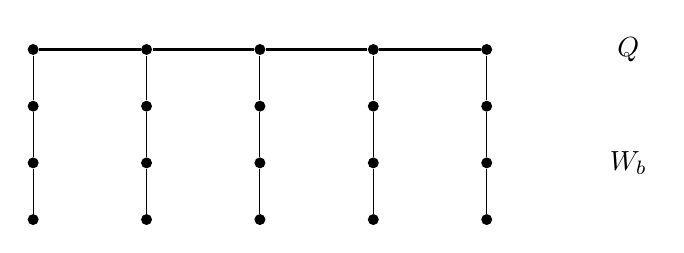
\begin{tikzpicture}[scale=0.9,every node/.style={circle,fill,inner sep=1.4pt}]
\foreach \i in {0,...,4}{ \node (q\i) at (1.6*\i,0) {}; }
\foreach \i in {0,...,3}{ \pgfmathtruncatemacro{\j}{\i+1} \draw[very thick] (q\i)--(q\j); }
\foreach \i in {0,...,4}{
  \node (a\i) at (1.6*\i,-0.8) {}; \node (b\i) at (1.6*\i,-1.6) {}; \node (c\i) at (1.6*\i,-2.4) {};
  \draw (q\i)--(a\i)--(b\i)--(c\i);}
\node[draw=none,fill=none] at (8.4,0) {$Q$};
\node[draw=none,fill=none] at (8.4,-1.6) {$W_b$};
\end{tikzpicture}
\caption{The comb used at the end of the proof: a geodesic $Q$ of the core $K$ with the pendant paths $W_b$ ($b\in Q$) attached. Here $|Q|=5$ and $m=3$.}\label{fig:comb}
\end{figure}

\begin{proof}[Proof of Theorem~\ref{thm:rooted}]
Let $K=F-\bigcup_{b\in B}W_b$. By Lemma~\ref{lem:prop}(i) and (iii), the sets $W_b$ are pairwise disjoint and disjoint from $B$, so $B\subseteq V(K)$. $K$ is connected: a geodesic of $F$ between two vertices of $K$ cannot enter any $W_b$, since it would have to leave through $b$ again. For $b\in B$ and $b'\ne b$, the vertex $b$ has no neighbour in $W_{b'}$: the only vertex outside $W_{b'}$ adjacent to $W_{b'}$ is $b'$, and $b\notin W_{b'}$ by Lemma~\ref{lem:prop}(i). Hence $N_K(b)=N_F(b)\setminus W_b\subseteq B$ by Lemma~\ref{lem:prop}(iv). Since $x\in B$ and $K$ is connected, $B=V(K)$. Thus $F$ consists of the connected graph $K$ together with a pendant path $W_b$ of length $m$ at every vertex $b$ of $K$.

Let $c$ be a centre of $K$. Every vertex of $K$ is within $\rad(K)$ of $c$, and every vertex of $W_b$ is within $d_K(c,b)+m\le\rad(K)+m$. So $\rad(F)\le\rad(K)+m$, and $\diam(K)\ge\rad(K)\ge k+1-m=t$.

Let $Q$ be a geodesic of $K$ with $\diam(K)+1\ge t+1$ vertices. Then $Q\cup\bigcup_{b\in Q}W_b$ is an induced tree of $F$ (Figure~\ref{fig:comb}). Indeed, $Q$ is an induced path of $K=F[V(K)]$, and each $W_b$ is attached only at $b$. Using $k+1=t+m$, its order is
\[
|Q|(m+1)\ \ge\ (t+1)(m+1)\ =\ 2(t+m)+(t-1)(m-1)\ \ge\ 2k+2 .
\]
This contradicts $\tr(F)\le2k+1$ (Lemma~\ref{lem:unroot}). Hence no counterexample exists.
\end{proof}

%======================================================================
\subsection{Proofs of the main results}\label{sec:main}
%======================================================================

\begin{proof}[Proof of Theorem~\ref{thm:cut}]
Let $c$ be a cut vertex and $r=\rad(G)$. List the components of $G-c$ by decreasing depth $e_1\ge e_2\ge\cdots$, where the depth of a component $A$ is $\max_{a\in A}d(c,a)\ge1$. Then $e_1=\ecc(c)\ge r$. Geodesics from $c$ into the two deepest components form an induced path on $e_1+e_2+1$ vertices. So we may assume $e_1+e_2+1\le 2r-1$, which gives $m:=e_2\le r-2$ and hence $r\ge3$.

Let $A_1,A_2$ be the two deepest components, let $H=G[A_1\cup\{c\}]$, and let $q$ be a geodesic of length $m$ from $c$ into $A_2$. Put $F=G[V(H)\cup V(q)]\cong H\plus_c P_m$. By Lemma~\ref{lem:sep}(a), for $z\in A_1\cup\{c\}$,
\[
\ecc_F(z)=\max\{\ecc_H(z),d(z,c)+e_2\}=\ecc_G(z)\ge r,
\]
while the vertices of $q$ other than $c$ have eccentricity at least $e_1+1\ge r+1$ in $F$. Hence $\rad(F)\ge r$.

Set $k=r-1$ and $t=r-m$, so that $2\le t\le k$ and $m=k-t+1$. By Lemma~\ref{lem:pendant}, $c$ is $(k,t)$-far in $H$, and Theorem~\ref{thm:rooted} applies to $(H,c,k,t)$. If (T) holds, then $\tr(G)\ge\tr(H)\ge 2k+2=2r$. If (R) holds, an induced tree $T\ni c$ of $H$ with $|T|\ge k+t+1=2r-m$, together with $V(q)$, is an induced tree of $G$ on at least $2r$ vertices (Lemma~\ref{lem:sep}(b)).
\end{proof}

\begin{proof}[Proof of Theorem~\ref{thm:84}]
Let $G$ be connected with $\delta(G)\ge1$; so $|V(G)|\ge2$ and $\rad(G)\ge1$.

If $\delta(G)\ge2$, a diametral geodesic is an induced path on $\diam(G)+1$ vertices. Hence $\tr(G)\ge\rad(G)+1>\rad(G)\ge 2\rad(G)/\delta(G)$.

Let $\delta(G)=1$. If $G=K_2$, then $\tr(G)=2=2\rad(G)$. Otherwise the neighbour of a vertex of degree one is a cut vertex, and Theorem~\ref{thm:cut} gives $\tr(G)\ge2\rad(G)=2\rad(G)/\delta(G)$.

Finally, the path on $2r$ vertices has $\delta=1$, radius $r$ and $\tr=2r$, so equality holds.
\end{proof}

\begin{proof}[Proof of Corollary~\ref{cor:2conn}]
A connected graph with at least three vertices that is not $2$-connected has a cut vertex. By Theorem~\ref{thm:cut} it then has $\tr(G)\ge2\rad(G)>2\rad(G)-1$.
\end{proof}

\begin{remark}
In the leaf case one can also go directly through Remark~\ref{rem:leaf}. If $u$ is a leaf with neighbour $w$ and $r=\rad(G)\ge2$, then Theorem~\ref{thm:rooted} with $k=t=r-1$, applied to $(G-u,w)$, gives either an induced tree on $2r$ vertices or a $w$-coherent tree on $2r-1$ vertices. In the second case adding $u$ gives a tree on $2r$ vertices.
\end{remark}

%======================================================================

\subsection{Questions beyond the proved radius statement}
\label{sec:open}
\begin{conjecture}[Path version]\label{conj:path}
Under the hypotheses of Theorem~\ref{thm:rooted}, either $\tr(G)\ge2k+2$,
or $x$ is an end of an induced path on at least $k+t+1$ vertices.
\end{conjecture}
This would imply the rooted induced-tree theorem. Our proof does not
establish it: the unrooting
equivalence used here does not preserve induced paths.
\begin{conjecture}\label{conj:sc}
If $G$ is connected and $\diam(G)>\rad(G)$, then $\tr(G)\ge2\rad(G)$.
\end{conjecture}
Every connected graph with a leaf and at least three vertices has
$\diam>\rad$; $K_2$ is an exception. The corresponding induced-path
statement fails on $C_4\circ K_1$ from Remark~\ref{rem:nopath}.
Neither conjecture is counted as a proved result. Even cycles and the
cocktail-party graphs $K_{2,2,\ldots,2}$ with at least two parts attain
$\tr(G)=2\rad(G)-1$; classifying the $2$-connected self-centred equality
graphs remains a separate question.

\paragraph{Acknowledgement of the proof framework.}
The neighbour-removal reductions follow the structure of the
Bacs\'o--Tuza induction \cite{BT90}, also formalised in \cite{Mak}.
The coherent-root condition, pendant-path equivalence, and propagation
argument are supplied explicitly here. The proof of 84 does not rely
on the historical induced-path theorem or on a computational census.
\section{Induced paths and radial circles: Conjecture 136}
\label{r3p:sec136}

For a center $c$ of a connected graph $G$, its \emph{radial circle} is
\[
 R(c)=\{v\in V(G):d_G(c,v)=\rad(G)\}.
\]
Write $R=\bigcup_c R(c)$, where the union is over all centers, and put
\[
 \Delta(R)=\max_{v\in R}\deg_G(v).
\]
Thus the degrees are measured in $G$, and all radial circles are included.
As in the source, $\operatorname{path}(G)$ is the number of vertices of a
largest induced path.

The shorter overlapping-cycle argument below incorporates the author-supplied
research notes~\cite{UserNotes}.

\begin{theorem}[WOWII Conjecture~136, finite girth]
\label{r3p:thm136}
Every finite simple connected graph $G$ containing a cycle satisfies
\begin{equation}
\label{r3p:bound136}
 \operatorname{path}(G)\geq
 \frac{1+\operatorname{girth}(G)}{\Delta(R)}.
\end{equation}
In particular, if every vertex of every radial circle is a leaf, then
$G$ has an induced path on at least $\operatorname{girth}(G)+1$ vertices.
\end{theorem}

\begin{proof}
Put $\ell=\operatorname{path}(G)$, $g=\operatorname{girth}(G)$,
$r=\rad(G)$, and $D=\Delta(R)$. A shortest cycle is induced, so deleting
one of its vertices gives $\ell\geq g-1$. If $D\geq2$, then
$D\ell\geq2(g-1)\geq g+1$, since $g\geq3$.
It therefore suffices to rule out $D=1$ and $\ell\leq g$.

Root a breadth-first spanning tree at a center. Every vertex at depth
$r$ is a leaf of $G$, because $D=1$. Since $G$ contains a cycle, the tree
has a non-tree edge, whose endpoints both have depth at most $r-1$.
This edge and its tree path form a cycle of length at most $2r-1$.
Consequently $g\leq2r-1$. The classical induced-path bound of
Erd\H{o}s, Saks and S\'os~\cite{ESS86} gives $\ell\geq2r-1$; hence
\begin{equation}
\label{r3p:forced}
 \ell=g=2r-1.
\end{equation}
Write $g=2k+1$ and $r=k+1$.

If $g=3$, then $r=2$. There is a leaf $z$, since every radial circle is
nonempty and consists of leaves. Its neighbor $u$ is not universal,
as that would give radius one. A shortest path from $u$ to a nonneighbor
starts $u,x,y$, where $uy\notin E(G)$. Thus $z,u,x,y$ is an induced
path on four vertices, a contradiction. We may assume $g\geq5$.

Fix a shortest cycle $C=c_0c_1\cdots c_{g-1}c_0$, with subscripts modulo
$g$. An outside vertex has at most one neighbor on $C$: two neighbors
and a shorter cycle arc would give a cycle of length at most
$k+2<g$. If a vertex has distance at least two from $C$, take vertices
$x,y,c_0$ on a shortest path to $C$, with $d_G(x,C)=2$.
Then
\[
 x,y,c_0,c_{g-1},c_{g-2},\ldots,c_2
\]
is an induced path on $g+1$ vertices. Therefore every outside vertex
has exactly one neighbor on $C$. The same argument applies to every
shortest cycle: \emph{each shortest cycle dominates $G$}.
Every vertex of $C$ has eccentricity at most $k+1=r$, so all its
vertices are centers.

Suppose first that there are no edges between outside vertices.
They are then leaves. Let $A\subseteq V(C)$ be their set of neighbors.
If two members of $A$ have cyclic distance two, the longer cycle arc
between them, with one leaf appended at each end, is an induced path
on $g+1$ vertices. Otherwise $A$ is independent in the graph joining
cycle vertices at cyclic distance two. Since $g$ is odd, this graph is
itself a $g$-cycle, and therefore $|A|\leq k$.
Each member of $A$ has exactly two cycle vertices at cyclic distance
$k$. At most $2|A|\leq2k$ cycle vertices can consequently be at
distance $k+1$ from a leaf. A remaining cycle vertex has eccentricity
at most $k$, contradicting $r=k+1$.

There must therefore be adjacent outside vertices $a,b$. Let $u,v$
be their respective cycle neighbors. If $u=v$, there is a triangle.
Otherwise a shorter $u$--$v$ arc of $C$, together with $u,a,b,v$,
gives a cycle of length at most $k+3$. Hence $2k+1=g\leq k+3$;
as $k\geq2$, we have $k=2$, $g=5$, and $r=3$.
The attachment vertices have cyclic distance two, so relabel them
$u=c_0$ and $v=c_2$. Then
\[
 C'=a,c_0,c_1,c_2,b,a
\]
is another shortest cycle and also dominates $G$.
All vertices of $C\cup C'$ are at distance at most two from $c_1$.
Since $c_1$ is a center and $r=3$, some vertex $w$ has distance three
from $c_1$. It lies outside $C\cup C'$ and is a leaf, because $D=1$.
Both cycles dominate $G$, so the unique neighbor of $w$ must belong to
$V(C)\cap V(C')=\{c_0,c_1,c_2\}$. Each of these vertices is within one
step of $c_1$, giving $d_G(c_1,w)\leq2$, a final contradiction.
Thus $\ell\geq g+1$ when $D=1$, completing the proof.
\end{proof}

\begin{remark}[Sharpness at every finite girth]
\label{r3p:sharpness}
For every integer $g\geq3$, attach one pendant leaf to each vertex of
$C_g$, obtaining $H=C_g\circ K_1$. Its girth is $g$. Its cycle vertices
have eccentricity $\lfloor g/2\rfloor+1$, while its leaves have
eccentricity $\lfloor g/2\rfloor+2$. Thus the centers are exactly the
cycle vertices, and every radial vertex is a leaf, giving $\Delta(R)=1$.
An induced path contains at most $g-1$ cycle vertices, since all $g$
would induce a cycle, and at most two pendant leaves, which can only
be its endpoints. Taking $g-1$ consecutive cycle vertices and the two
pendant leaves at their ends attains this bound. Hence
$\operatorname{path}(H)=g+1$, and \eqref{r3p:bound136} is sharp at every
finite girth.
\end{remark}

\begin{remark}[Acyclic graphs and the domain of the statement]
\label{r3p:scope}
The source defines girth by the order of a smallest cycle, without
specifying an acyclic value in that definition. Theorem~\ref{r3p:thm136}
therefore treats finite girth explicitly. If girth is assigned the value
zero on trees, every nontrivial tree also satisfies
\eqref{r3p:bound136}, since $\Delta(R)\geq1$ and
$\operatorname{path}(G)\geq2$. If instead the acyclic value is $+\infty$,
the unqualified inequality is false on trees and must retain the
finite-girth restriction. For $K_1$, $\Delta(R)=0$, so the displayed
quotient is undefined.
\end{remark}

\section{Rooted extensions and statements 178 and 179}\label{sec:extensions}

\begin{theorem}\label{thm:core}
Every nonempty finite simple graph satisfies
\begin{equation}\label{eq:core}
\boxed{b(G)\ge s(G)+i(G)\ge s(G)+\gamma(G).}
\end{equation}
Connectivity is unnecessary.
\end{theorem}
\begin{proof}
Choose a vertex $x$ and an independent set $S\subseteq N_G(x)$ of size
$s(G)$. Extend $\{x\}$ to a maximal independent set $D$ of $G$.
Every vertex of $S$ is adjacent to $x\in D$, so $S\cap D=\varnothing$.
The induced subgraph $G[S\cup D]$ is bipartite with independent colour
classes $S$ and $D$. Moreover, maximality makes $D$ dominating, and hence
$|D|\ge i(G)\ge\gamma(G)$. Therefore
$b(G)\ge |S|+|D|\ge s(G)+i(G)$.
\end{proof}

\begin{lemma}[Tree extension]\label{lem:extend}
In a connected graph, every tree subgraph with at least two vertices can
be extended to a spanning tree without decreasing its number of leaves.
\end{lemma}
\begin{proof}
While the tree is not spanning, add one edge from its vertex set to an
outside vertex, together with that vertex. Such an edge exists by
connectivity. If the attachment vertex was a leaf, the new leaf replaces
it; otherwise the leaf count increases. Repetition finishes the extension.
\end{proof}

\begin{lemma}\label{lem:leafbounds}
For connected $G$ of order at least two,
\begin{equation}\label{eq:leafbounds}
L(G)\ge\Delta(G),\qquad L(G)\ge q_E(G)-2.
\end{equation}
\end{lemma}
\begin{proof}
All edges incident with a maximum-degree vertex form a star. It has at
least $\Delta(G)$ leaves, including the case $\Delta=1$, when $G=K_2$.
Apply Lemma~\ref{lem:extend}.

For an edge $uv$ attaining $q_E$, take $uv$ and attach each vertex of
$(N(u)\cup N(v))\setminus\{u,v\}$ to exactly one adjacent endpoint.
This is a tree in which all $q_E-2$ vertices other than $u,v$ are leaves.
Extend it by the same lemma.
\end{proof}

The original statements are
\begin{align}
L+b&\ge s+q_E,&&\text{No. 178},\label{eq:178}\\
L+b&\ge\Delta+s+\gamma,&&\text{No. 179}.\label{eq:179}
\end{align}
The latter also appears in West's problem list \cite{West}.

\begin{theorem}\label{thm:178179}
Every connected graph of order at least two satisfies
\begin{align}
\boxed{L+b\ge\Delta+s+i,}\label{eq:179strong}\\
\boxed{L+b\ge s+q_E+\max\{0,i-2\}.}\label{eq:178strong}
\end{align}
Consequently both \eqref{eq:178} and \eqref{eq:179} hold.
\end{theorem}
\begin{proof}
The first inequality is the sum of $L\ge\Delta$ and $b\ge s+i$.
If $i\ge2$, adding $L\ge q_E-2$ and $b\ge s+i$ gives the second.
If $i=1$, a singleton independent dominating set is a universal vertex.
Its spanning star gives $L\ge n-1$, while $b\ge s+1$ and $q_E\le n$.
Hence $L+b\ge n+s\ge q_E+s$, as required. Finally, $i\ge\gamma$.
\end{proof}

\begin{proposition}[Sharpness]\label{prop:k2m}
For every $m\ge2$, the graph $K_{2,m}$ attains equality in \eqref{eq:core},
\eqref{eq:179strong}, \eqref{eq:178strong}, and both original inequalities.
\end{proposition}
\begin{proof}
Its parameters are
\[
b=m+2,\quad s=\Delta=m,\quad i=\gamma=2,\quad q_E=m+2,\quad L=m.
\]
The assertions other than $L=m$ follow directly from its two independent
parts and the absence of a universal vertex. If its parts are
$\{a_1,a_2\}$ and $\{c_1,\ldots,c_m\}$, the edges $a_1c_j$ together
with $a_2c_1$ give a spanning tree with $m$ leaves. A spanning tree with
$m+1$ leaves would be a star, impossible without a universal vertex.
Substitution proves equality. For $K_2$, by contrast, both original
inequalities have left side four and right side three.
\end{proof}

\section{Aggregate local independence: statement 111}\label{sec:111}

Let $S$ be the set of maximum-degree vertices of $\overline G$, equivalently
the minimum-degree vertices of $G$. Put
\[
A=N_{\overline G}(S),\qquad q=|A|,\qquad
a=\alpha(G),\qquad E_\lambda=\sum_{v\in V(G)}(\lambda_G(v)-1).
\]
The letter $q$ in this section refers to this complement-neighbourhood
size, not to the edge-neighbourhood parameter $q_E$.
The printed assertion is
\begin{equation}\label{eq:111}
\boxed{\alpha(G)\le
\left\lceil1+|N_{\overline G}(S)|
\left(\frac1n\sum_v\lambda_G(v)-1\right)\right\rceil.}
\end{equation}
Here the neighbourhood of $S$ is explicitly taken in the complement,
whereas $\lambda_G$ is evaluated in $G$.

\begin{lemma}\label{lem:sumlambda}
For every connected graph of order at least two,
$E_\lambda\ge\alpha(G)-1$.
\end{lemma}
\begin{proof}
Choose a maximum independent set $I$ of size $a$ and let $J=V(G)\setminus I$.
Let $H$ be the spanning bipartite graph retaining exactly the edges of $G$
between $I$ and $J$. Every vertex of $J$ has a neighbour in $I$ by
maximality, and every vertex of $I$ has a neighbour in $J$ by connectivity.
Thus $H$ has no isolated vertices. If $c$ is its number of components and
$m_H$ its number of edges, then $m_H\ge n-c$.
For $v\in J$ we have $\lambda_G(v)\ge d_H(v)$, and for $v\in I$ we
have $\lambda_G(v)\ge1$. Consequently
\[
\sum_v\lambda_G(v)\ge a+m_H\ge a+n-c.
\]
If $c=1$, this suffices.

Suppose $c\ge2$. Each component of $H$ has a $G$-edge to a different
component, since $G$ is connected. Every such edge joins two vertices
of $J$. In each component choose an endpoint $v\in J$ of one such edge,
and write $u\in J$ for its neighbour in the other component.
The set $N_H(v)\cup\{u\}$ is independent: an edge from $u$ to
$N_H(v)\subseteq I$ would put $u$ and $v$ in the same component of $H$.
Thus $\lambda_G(v)\ge d_H(v)+1$ for one distinct vertex in each
component. These $c$ additional units give
\[
\sum_v\lambda_G(v)\ge a+m_H+c\ge a+n.
\]
In this case even $E_\lambda\ge a$ holds, proving the lemma.
\end{proof}

\begin{lemma}\label{lem:qbounds}
If $G$ is connected and $a\ge2$, then
\begin{equation}\label{eq:qbounds}
q\ge a,\qquad E_\lambda\ge(a-1)n-aq+a-1.
\end{equation}
\end{lemma}
\begin{proof}
Write $\delta=\delta(G)$. Since every $s\in S$ has complement degree
$n-1-\delta$, we have $q\ge n-1-\delta$. Suppose $q\le a-1$.
Then $\delta\ge n-a$, while each vertex of a maximum independent set
$I$ has degree at most $n-a$. Hence $\delta=n-a$, every vertex of $I$
belongs to $S$, and $q=a-1$. As $a\ge2$, each vertex of $I$ is
nonadjacent to another vertex of $I\subseteq S$ and therefore belongs
to $A$. This contradicts $q=a-1$, proving $q\ge a$.

For the second inequality let $B=V(G)\setminus A$ and $r=|B|=n-q$.
Each $s\in S$ is adjacent in $G$ to every vertex of $B$ other than
possibly itself, so $\delta\ge r-1$.
If $\delta\ge r$, then $\sum_{v\in I}d_G(v)\ge ar$.
If $\delta=r-1$, then $S\subseteq B$: otherwise a vertex of $S$
outside $B$ would have all $r$ vertices of $B$ as neighbours.
Moreover, $S$ is a clique, because vertices of $B$ have no complement
neighbour in $S$. Thus $I$ contains at most one minimum-degree vertex;
all its other vertices have degree at least $r$. It follows that
\[
\sum_{v\in I}d_G(v)\ge ar-1.
\]
This estimate holds in both cases. As in Lemma~\ref{lem:sumlambda},
\[
\sum_v\lambda_G(v)\ge a+\sum_{v\in I}d_G(v)\ge a+ar-1.
\]
Subtracting $n$ and using $r=n-q$ proves the claim. If $r=0$, only
the first degree case is needed.
\end{proof}

\begin{theorem}\label{thm:111}
Every connected finite simple graph satisfies statement 111,
namely \eqref{eq:111}.
\end{theorem}
\begin{proof}
For $K_1$, $q=0$ and both sides of \eqref{eq:111} equal one.
If $n\ge2$ and $a=1$, the graph is complete, $q=E_\lambda=0$, and
the result again follows. Assume $a\ge2$. It is enough to prove
\begin{equation}\label{eq:strict111}
qE_\lambda>n(a-2),
\end{equation}
because then $1+qE_\lambda/n>a-1$ and its ceiling is at least $a$.

If $n=a+1$, connectivity forces $G$ to be a star: the sole vertex outside
a maximum independent set must be adjacent to all of it. Then
$q=a$, $E_\lambda=a-1$, and
\[
\frac{qE_\lambda}{n}=\frac{a(a-1)}{a+1}
=a-2+\frac{2}{a+1}>a-2.
\]
Otherwise $n\ge a+2$. Put $q_0=(a-1)n/a$.
For $q\ge q_0$, Lemma~\ref{lem:sumlambda} yields
\[
qE_\lambda\ge q(a-1)\ge\frac{(a-1)^2n}{a}
=n(a-2)+\frac{n}{a}>n(a-2).
\]
For $q<q_0$, Lemma~\ref{lem:qbounds} places $q$ in $[a,q_0)$, which
is empty if $q_0<a$. Consider the concave quadratic
\[
f(x)=x\bigl((a-1)n-ax+a-1\bigr)-n(a-2).
\]
By the same lemma, $qE_\lambda-n(a-2)\ge f(q)$. Its endpoint values are
\begin{align*}
f(q_0)&=n/a>0,\\
f(a)&=(a^2-2a+2)n-a(a^2-a+1)\\
&\ge(a^2-2a+2)(a+2)-a(a^2-a+1)\\
&=a^2-3a+4=(a-1)(a-2)+2>0.
\end{align*}
A concave function on an interval is at least the smaller of its endpoint
values. Thus $f(q)>0$, proving \eqref{eq:strict111} and the theorem.
\end{proof}

\section{Leaves, cliques, simplicial vertices, and parity}\label{sec:leaves}

\subsection{Statement 161: local independence in the complement}

\begin{theorem}\label{thm:161}
Every connected graph satisfies
\begin{equation}\label{eq:161}
L(G)\ge s(\overline G).
\end{equation}
For connected $n\ge2$ the stronger intermediate bound
$s(\overline G)\le\Delta(G)\le L(G)$ holds. Also, every connected
noncomplete graph satisfies $L(G)\ge\omega(G)$.
\end{theorem}
\begin{proof}
An independent set $Q\subseteq N_{\overline G}(v)$ is a proper clique
of $G$. If $Q$ is nonempty, connectivity supplies an edge $xy$ with
$x\in Q$ and $y\notin Q$. Then $d_G(x)\ge|Q|$, since $x$ is adjacent
to all other vertices of $Q$ and to $y$. Taking the largest possible $Q$
gives $s(\overline G)\le\Delta(G)$, and Lemma~\ref{lem:leafbounds}
finishes the proof for $n\ge2$. For $K_1$, both sides of \eqref{eq:161}
are zero. The same clique argument applied to a maximum clique in a
connected noncomplete graph proves $\omega(G)\le\Delta(G)\le L(G)$.
\end{proof}

\begin{remark}[Sharpness]
Attach a path of length two to one vertex of $K_r$, where $r\ge2$.
The new terminal vertex is nonadjacent to the entire $K_r$, so
$s(\overline G)\ge r$. The theorem gives $L\ge r$.
The graph has $r+2$ vertices and no universal vertex, so it has no spanning
star and $L\le r$. Thus $L=s(\overline G)=r$.
\end{remark}

\subsection{Statement 162: preserving all simplicial vertices}

A vertex is \emph{simplicial} when its open neighbourhood induces a clique.
In a connected graph of order at least two, this is equivalent to
$\lambda_G(v)=1$.

\begin{lemma}\label{lem:simplicial}
If $G$ is connected and noncomplete, its nonsimplicial vertices form a
nonempty connected dominating set. Consequently, if $Q$ is its set of
simplicial vertices, then $L(G)\ge |Q|$.
\end{lemma}
\begin{proof}
Every internal vertex of a shortest path is nonsimplicial: its predecessor
and successor are nonadjacent neighbours, since an edge between them would
shorten the path. A shortest path between two nonadjacent vertices shows
that the set $D$ of nonsimplicial vertices is nonempty. Shortest paths
between vertices of $D$ lie entirely in $D$, so $G[D]$ is connected.
For $q\notin D$, a shortest path from $q$ to $D$ has length one; otherwise
its first internal vertex already belongs to $D$, a contradiction.
Thus $D$ dominates $Q=V(G)\setminus D$.

Take a spanning tree of $G[D]$ and attach each vertex of $Q$ to one
neighbour in $D$. If $|D|=1$, start from that single vertex. Every vertex
of $Q$ is a leaf of the resulting spanning tree, proving $L(G)\ge|Q|$.
\end{proof}

\begin{theorem}\label{thm:162}
For every connected graph of order at least two,
\begin{equation}\label{eq:162}
L(G)\ge
\bigl|\{v:\lambda_G(v)=\min_w\lambda_G(w)\}\bigr|
\left\lfloor\frac1{\delta(G)}\right\rfloor.
\end{equation}
\end{theorem}
\begin{proof}
If $\delta\ge2$, the right side is zero. If $\delta=1$, a pendant
vertex shows that $\min_v\lambda_G(v)=1$. Its frequency is exactly the
number of simplicial vertices. For $n\ge3$, a connected graph with
$\delta=1$ is noncomplete, so Lemma~\ref{lem:simplicial} applies.
For $K_2$, both sides equal two. At $K_1$, the printed denominator is zero,
so the formula itself is undefined.
\end{proof}

\subsection{Statement 169: a breadth-first parity bound}

\begin{theorem}\label{thm:169}
Every connected graph of order $n\ge2$ satisfies
\begin{equation}\label{eq:169strong}
\boxed{L(G)\ge1+\max_{v\in V(G)}|2e_G(v)-n|.}
\end{equation}
In particular,
\begin{equation}\label{eq:169}
L(G)\ge1+\max_v e_G(v)-\min_v e_G(v).
\end{equation}
\end{theorem}
\begin{proof}
First let $T$ be a tree with at least two vertices and bipartition sizes
$a\ge b$. If $\ell_A$ of its leaves lie in the larger part $A$, then
\[
a+b-1=\sum_{x\in A}d_T(x)\ge2(a-\ell_A)+\ell_A.
\]
Thus $\ell(T)\ge\ell_A\ge a-b+1$.

For any root $v$, a breadth-first spanning tree preserves its distances
to all vertices. The two parts of this tree therefore have sizes
$e_G(v)$ and $n-e_G(v)$. Applying the preceding estimate gives
$L(G)\ge1+|2e_G(v)-n|$. Maximizing over $v$ proves
\eqref{eq:169strong}. Finally, if $E=\max_v e_G(v)$ and
$r=\min_v e_G(v)$, then
\[
E-r\le\frac{|2E-n|+|2r-n|}{2}
\le\max_v|2e_G(v)-n|,
\]
which proves \eqref{eq:169}.
\end{proof}

\begin{remark}[The printed singleton exception and equality]
The archived wording of 169 says only ``connected''. With degree-one
leaves, $K_1$ has $L=0$, whereas the right side of \eqref{eq:169} is one.
Thus the literal unrestricted formulation is false at $K_1$; the theorem
settles its entire nontrivial connected-graph range. If the unique vertex
of $K_1$ is instead counted as a leaf, that convention removes the exception.
For each star $K_{1,r}$ with $r\ge2$, $\max e=r$, $\min e=1$, and
$L=r$, so \eqref{eq:169} is sharp. The stronger bound is also sharp on
$K_n$ for $n\ge3$.
\end{remark}

\section{A counterexample to the radius bound for spanning-tree leaves}
\label{r7leaf:sec166}

The counterexample in this section was supplied in the author-supplied research
materials \texttt{WOWII\_results\_2026-10-26.md} and
\texttt{wowii\_counterexamples.py}.  We give an independent structural
verification.  Thus the discovery is attributed to those supplied materials;
the following argument provides a self-contained certificate.

For a connected graph $G$, let $L(G)$ denote the maximum number of leaves in
a spanning tree, let $M$ be its maximum-degree vertex set, and write
$\partial M=N_G(M)\setminus M$.  WOWII~166 asserts
\[
 L(G)\ge \frac{|\partial M|}{\sqrt{\operatorname{rad}(G)}}.
\]

\begin{theorem}\label{r7leaf:counter166}
There is a connected simple graph $G$ with
\[
 |V(G)|=20,\qquad |E(G)|=23,\qquad
 \Delta(G)=3,\qquad |\partial M|=14,\qquad
 \operatorname{rad}(G)=5,\qquad L(G)=6.
\]
Consequently, WOWII~166 is false, since
\[
 L(G)^2\operatorname{rad}(G)=180<196=|\partial M|^2.
\]
\end{theorem}

\begin{proof}
Begin with six distinct branch vertices $a,a',p,q,c,c'$.
Join $a$ to $a'$ by two internally disjoint paths of length two, whose
internal vertices are $s,s'$.  Similarly join $c$ to $c'$ by two paths of
length two, with internal vertices $t,t'$.  Finally, replace each of
\[
 ap,\quad a'q,\quad pq,\quad pc,\quad qc'
\]
by a path of length three.  All internal vertices used in this construction
are distinct.  This defines a connected simple graph with
$6+4+2\cdot5=20$ vertices and $4\cdot2+5\cdot3=23$ edges.
Exactly the six branch vertices have degree three; every other vertex has
degree two and is adjacent to a branch vertex.  Hence $M$ consists of the
six branch vertices and $\partial M$ consists of the other fourteen.

For any subcubic tree $T$, the degree sum gives
\[
 |\{v:\deg_T(v)=1\}|=2+|\{v:\deg_T(v)=3\}|.
\]
A spanning tree of $G$ must omit an edge of the four-cycle
$a,s,a',s',a$.  Every edge of that cycle is incident with $a$ or $a'$, so
at least one of these two vertices has degree at most two in the spanning
tree.  The disjoint four-cycle $c,t,c',t',c$ forces the same conclusion for
$c,c'$.  Thus at most four branch vertices can have tree degree three, and
$L(G)\le6$.

For equality, delete the four edges
\[
 as,\quad as',\quad ct,\quad ct'.
\]
The five paths of length three form a subdivision of the tree on the six
branch vertices with edge set $\{ap,a'q,pq,pc,qc'\}$.
The remaining four vertices $s,s',t,t'$ are attached as leaves to $a'$ or
$c'$.  The resulting graph is therefore a spanning tree, with precisely
$a,c,s,s',t,t'$ as leaves.  Hence $L(G)=6$.

It remains to verify the radius.  The distance from $s$ to $t$ is eight.
There are exactly two shortest $s$--$t$ paths: one runs through $a,p,c$,
and the other through $a',q,c'$.  Indeed, in the weighted six-vertex core,
the distances from $a$ to $c$ and from $a'$ to $c'$ are six, while the
crossed distances from $a$ to $c'$ and from $a'$ to $c$ are eight.
The midpoints of the two length-eight geodesics are therefore $p$ and $q$.
If a vertex had eccentricity at most four, it would be a midpoint of an
$s$--$t$ geodesic and hence equal to $p$ or $q$.
But $d_G(p,a')=d_G(q,a)=5$, so neither has eccentricity at most four.
On the other hand every vertex is within distance five of $p$:
its distances to $a,a',q,c,c'$ are $3,5,3,3,5$, respectively, and direct
inspection of the nine subdivided paths gives the same upper bound for
the internal vertices.  Thus $\operatorname{rad}(G)=5$.
\end{proof}

\begin{remark}\label{r7leaf:verification166}
The supplied graph6 encoding is
\begin{verbatim}
S`?AG?_E??G_B????KC@????@@G?o??QO
\end{verbatim}
An independent integer-arithmetic checker enumerated all
$\binom{23}{4}=8855$ four-edge deletion sets.  Exactly $1456$ yield spanning
trees: $324$ have four leaves, $824$ have five leaves, and $308$ have six
leaves.  Breadth-first searches independently verify the radius and the
maximum-degree boundary.  These calculations confirm the structural
proof; they are not needed for it.  No claim of smallest possible order
is made.
\end{remark}

\section{Pendant extensions and statement 432b}\label{sec:432}

Let $P$ be the set of pendant vertices and $S=N_G(P)$ the set of support
vertices. The source's multiplier ``\texttt{\_bipartite}'' is the
bipartite characteristic function $\bip(G)$.

\begin{theorem}\label{thm:432}
Every connected graph with $n>3$ satisfies
\begin{equation}\label{eq:432}
\boxed{i(G)\le |V(G)\setminus N_G(P)|+
\bip(G)\min_v\bigl(e_G(v)-o_G(v)\bigr).}
\end{equation}
\end{theorem}
\begin{proof}
The pendant set $P$ is independent: adjacent pendant vertices would form
an entire component $K_2$. Extend $P$ to a maximal independent set $I$.
Since $P\subseteq I$, the set $I$ avoids all of $S=N(P)$. It is
dominating, so
\begin{equation}\label{eq:pendantbound}
i(G)\le |I|\le n-|S|.
\end{equation}
This proves \eqref{eq:432} when $G$ is not bipartite.

If $G$ is bipartite, let its parts be $A,B$ with $a=|A|\le b=|B|$.
Connectivity ensures that each part is independently dominating, so
$i(G)\le a$. Parity of distance gives
\[
\min_v(e_G(v)-o_G(v))=a-b.
\]
Each support vertex in $B$ has a pendant neighbour in $A$, and different
support vertices have different such neighbours. The support vertices
in $A$ are disjoint from its pendant vertices, since $G$ is connected
and has more than two vertices. Hence
\[
|S|=|S\cap A|+|S\cap B|
\le |S\cap A|+|P\cap A|\le a.
\]
The right side of \eqref{eq:432} is therefore
$n-|S|+a-b=2a-|S|\ge a\ge i(G)$.
\end{proof}

\section{Total domination and spanning-tree leaves}
\label{sec:totaldom}

We prove WOWII Conjectures~258 and~261. Throughout this section, $G$ is a
finite simple connected graph of order $n\geq 2$, and $L=L(G)$ is the
maximum number of degree-one leaves in a spanning tree of $G$. Write
$t=\gamma_t(G)$ for the total domination number: the minimum cardinality
of a set $D\subseteq V(G)$ such that every vertex of $G$, including every
member of $D$, has a neighbour in $D$. Thus $t\geq 2$ and $L\geq 2$.
We also write $\gamma_c(G)$ for the minimum cardinality of a connected
dominating set. The restriction $n\geq 2$ excludes the isolated graph,
which has no total dominating set.

\begin{lemma}[Connecting a total dominating set]
\label{lem:newtd-connector}
For every such graph,
\begin{equation}
\label{eq:newtd-connector}
 \gamma_c(G)\leq 2t-2,
 \qquad L\geq n-2t+2,
 \qquad n\leq L+2t-2.
\end{equation}
\end{lemma}

\begin{proof}
Let $D$ be a total dominating set of cardinality $t$, and let
$C_1,\ldots,C_c$ be the components of $G[D]$. Since $G[D]$ has no isolated
vertices, $2c\leq t$. Assign each vertex outside $D$ to one component
containing a neighbour of that vertex. Together with $C_i$, the vertices
assigned to $C_i$ form a connected vertex class $X_i$. The classes
$X_1,\ldots,X_c$ partition $V(G)$, so their quotient graph is connected.

Choose a spanning tree of this quotient. For each of its $c-1$ edges,
choose one edge of $G$ joining the corresponding classes. Let $Q$ consist
of $D$ and all endpoints of these chosen edges. Then
\[
 |Q|\leq t+2(c-1)\leq 2t-2.
\]
Every retained endpoint outside $D$ is adjacent to its assigned
component, and the chosen cross edges join these components along the
quotient tree. Consequently $G[Q]$ is connected. It is also dominating,
since $Q$ contains $D$. This proves the bound on $\gamma_c(G)$.

Take a spanning tree of $G[Q]$, and attach each vertex outside $Q$ by one
edge to a neighbour in $Q$. The resulting graph is a spanning tree of $G$,
and every vertex outside $Q$ is a leaf. Hence
\[
 L\geq n-|Q|\geq n-2t+2.
\]
Rearranging gives the last inequality. This construction also applies
to $K_2$; it does not require an identity between $L$ and $n-\gamma_c(G)$.
\end{proof}

We shall also use two elementary observations. A tree subgraph can be
extended to a spanning tree without decreasing its number of leaves:
add vertices one at a time, each by a single edge to the existing tree.
In particular, extending a star gives $L\geq\Delta(G)$. Thus $L=2$
forces $G$ to be a path or a cycle. For these graphs,
\begin{equation}
\label{eq:newtd-degree-two}
 t\geq \left\lceil\frac n2\right\rceil,
\end{equation}
since a total dominating set $D$ satisfies
$n\leq\sum_{x\in D}\deg(x)\leq 2t$.

\begin{theorem}[WOWII Conjecture~258]
\label{thm:newtd-258}
Let
\[
 e_{\max}(G)=\max_{v\in V(G)}
 \bigl|\{u\in V(G):d_G(u,v)\text{ is even}\}\bigr|,
\]
where the vertex $v$ itself is counted. Then
\begin{equation}
\label{eq:newtd-258}
 \gamma_t(G)\geq\frac{2e_{\max}(G)}{L(G)}.
\end{equation}
\end{theorem}

\begin{proof}
Put $e=e_{\max}(G)$. It suffices to prove $tL\geq 2e$.
For $G=K_2$, we have $t=L=2$ and $e=1$, so the assertion holds.
Assume henceforth that $n\geq 3$.

First suppose $L=2$. Then $G$ is a path or a cycle. A path has
$e=\lceil n/2\rceil$, and an even cycle has $e=n/2$. On an odd cycle
$C_{2r+1}$, every vertex has
$1+2\lfloor r/2\rfloor\leq r+1=\lceil n/2\rceil$ vertices at even
distance. Thus $e\leq\lceil n/2\rceil\leq t$ by
\eqref{eq:newtd-degree-two}, giving $tL=2t\geq 2e$.

We may now assume $L\geq 3$. Suppose next that $t=2$. The two vertices
of a total dominating set are adjacent, so they form a connected
dominating set. Attaching all remaining vertices to this edge gives
$L\geq n-2$. If $e\leq n-2$, this already gives $L\geq e$ and hence
$tL\geq 2e$.

The only remaining possibility in this case is $e=n-1$: every vertex
has a neighbour at odd distance, so $e\leq n-1$. Choose a vertex $v$
with exactly one odd-distance vertex, say $w$. Every neighbour of $v$
is at odd distance, so $w$ is its unique neighbour. There is no vertex
at distance at least three from $v$, since a shortest path to such a
vertex would contain a second odd-distance vertex in its third layer.
Every vertex other than $v,w$ therefore lies at distance two from $v$
and is adjacent to $w$. Thus $w$ is universal, and its spanning star
has $n-1=e$ leaves. Again $tL\geq 2e$.

It remains to consider $t\geq 3$ and $L\geq 3$. We claim that
\begin{equation}
\label{eq:newtd-product}
 (t-1)L\geq n-1.
\end{equation}
If $n\leq 2t$, then
\[
 (t-1)L\geq 3t-3\geq 2t-1\geq n-1.
\]
If $n\geq 2t+1$, Lemma~\ref{lem:newtd-connector} gives
\begin{align*}
 (t-1)L-(n-1)
 &\geq (t-1)(n-2t+2)-(n-1)\\
 &= (t-2)(n-2t)-1\\
 &\geq t-3\geq 0.
\end{align*}
This proves \eqref{eq:newtd-product}. The previously established parity
bound \eqref{eq:169strong} gives $2e\leq n+L-1$. Therefore
\[
 tL=(t-1)L+L\geq n+L-1\geq 2e,
\]
as required.
\end{proof}

\begin{theorem}[WOWII Conjecture~261]
\label{thm:newtd-261}
Let $S=\{v\in V(G):\deg(v)=2\}$. With $N(S)$ denoting the union of the
open neighbourhoods of the vertices in $S$, we have
\begin{equation}
\label{eq:newtd-261}
 \gamma_t(G)\geq\frac{2|N(S)\setminus S|}{L(G)}.
\end{equation}
\end{theorem}

\begin{proof}
Put $s=|S|$ and $k=|N(S)\setminus S|$. We must prove $tL\geq 2k$.
For $K_2$, the set $S$ is empty, so the assertion is immediate.
Assume henceforth that $n\geq 3$.

Every vertex counted by $k$ is incident with an edge joining it to $S$.
Counting these edges at their endpoints in $S$ gives $k\leq 2s$.
Also $k\leq n-s$. Adding the first inequality to twice the second yields
\begin{equation}
\label{eq:newtd-boundary}
 k\leq\min\{2s,n-s\},\qquad 3k\leq 2n.
\end{equation}

Suppose first that $L\geq 4$. By Lemma~\ref{lem:newtd-connector},
\begin{align*}
 tL-(2n-4)
 &\geq tL-2(L+2t-2)+4\\
 &= (t-2)(L-4)\geq 0.
\end{align*}
If $s\geq 2$, then
\[
 2k\leq 2(n-s)\leq 2n-4\leq tL.
\]
If $s\leq 1$, then $k\leq 2$ and $tL\geq 8\geq 2k$.
This settles all cases with $L\geq 4$.

Suppose now that $L=3$. The connector bound gives $n\leq 2t+1$.
For $t\geq 4$, \eqref{eq:newtd-boundary} implies
\[
 2k\leq\frac{4n}{3}\leq\frac{8t+4}{3}\leq 3t=tL.
\]
For $t=2$, we have $n\leq 5$ and
$k\leq\lfloor 2n/3\rfloor\leq 3$, whence $2k\leq 6=tL$.
For $t=3$, we have $n\leq 7$ and
$k\leq\lfloor 2n/3\rfloor\leq 4$, whence $2k\leq 8<9=tL$.

Finally, suppose $L=2$. Then $G$ is a path or a cycle. For a cycle,
$S=V(G)$ and $k=0$. For a path, the only vertices outside $S$ are its
two endpoints, so $k\leq 2$. Hence $2k\leq 4\leq tL$ in either case.
All possible values of $L$ and $t$ have now been covered.
\end{proof}
\section{Total domination and vertex boundaries: 259 and 260}
\label{r3td:section}

All graphs in this section are finite and simple. For a connected graph
$G$ of order $n\ge2$, let $t=\gamma_t(G)$ be its total domination number,
$\gamma(G)$ its domination number, and $L=L(G)$ the maximum number of
leaves in a spanning tree. A leaf has degree one in that tree. A set $D$
is total dominating when every vertex of $G$ has a neighbor in $D$,
including every vertex of $D$ itself. Write $\gamma_c(G)$ for the minimum
cardinality of a connected dominating set. For $S\subseteq V(G)$, write
$N(S)=\bigcup_{v\in S}N(v)$, $N[S]=S\cup N(S)$, and
$\partial S=N(S)\setminus S$.

We prove 259 and 260 through a bound that applies to every vertex
boundary when $L\ge3$. This also gives a common strengthening of those
two conjectures and 261.

\begin{lemma}[The parity-sensitive connector bound]
\label{r3td:connector}
Every connected graph of order at least two satisfies
\[
 \gamma_c(G)\le t+2\lfloor t/2\rfloor-2,
 \qquad n\le L+t+2\lfloor t/2\rfloor-2.
\]
In particular, $n\le L+2t-2$, with the improvement
$n\le L+2t-3$ when $t$ is odd.
\end{lemma}
\begin{proof}
Take a total dominating set $D$ of size $t$. Its induced subgraph has no
isolated vertices, so its number $c$ of components is at most
$\lfloor t/2\rfloor$. Assign each vertex outside $D$ to one component
containing a neighbor of that vertex. This partitions $V(G)$ into $c$
connected classes, one for each component of $G[D]$. The quotient of
these classes is connected. Choose a spanning tree of the quotient and
one realizing edge of $G$ for each of its $c-1$ edges. Adjoin the endpoints
of these edges to $D$, obtaining a set $Q$ with
\[
 |Q|\le t+2(c-1)\le t+2\lfloor t/2\rfloor-2.
\]
Every added endpoint outside $D$ is adjacent to its assigned component,
and the chosen edges connect these components. Thus $Q$ is connected
and dominating. A spanning tree of $G[Q]$, with each vertex outside $Q$
attached by one edge to $Q$, has at least $n-|Q|$ leaves. This proves both
bounds, including when $G=K_2$.
\end{proof}

\begin{theorem}[A bound for every vertex boundary]
\label{r3td:boundary}
If $G$ is connected and $L(G)\ge3$, then
\begin{equation}
\label{r3td:general}
 \gamma_t(G)L(G)\ge
 2\max_{S\subseteq V(G)}|\partial S|
 =2\bigl(n-\gamma(G)\bigr).
\end{equation}
\end{theorem}
\begin{proof}
Fix $S\subseteq V(G)$, and put $s=|S|$ and $k=|\partial S|$. A star at
a maximum-degree vertex extends to a spanning tree without decreasing
its number of leaves, so $\Delta(G)\le L$. If $s=0$, then $k=0$. If
$s=1$, then $k\le\Delta(G)\le L$ and $t\ge2$ gives $tL\ge2k$. Hence
we may assume $s\ge2$.

First suppose $L\ge4$. By Lemma~\ref{r3td:connector},
\[
 tL-(2n-4)
 \ge tL-2(L+2t-2)+4
 =(t-2)(L-4)\ge0.
\]
Since $k\le n-s\le n-2$, this proves $tL\ge2k$.

It remains to consider $L=3$. Now $\Delta(G)\le3$. Counting the edges
from $S$ to its boundary gives $k\le3s$, while disjointness gives
$k\le n-s$. Thus
\[
 4k\le3n,\qquad k\le\left\lfloor\frac{3n}{4}\right\rfloor.
\]
If $t$ is odd, the improved connector bound gives $n\le2t$, whence
$2k\le3n/2\le3t=tL$. If $t$ is even, it gives $n\le2t+1$, and
\[
 k\le\left\lfloor\frac{3(2t+1)}4\right\rfloor
 =\frac{3t}{2}.
\]
Again $2k\le3t=tL$. This proves the inequality for every $S$.

For completeness, the maximum boundary size is exactly $n-\gamma(G)$.
For any $S$, the set $S\cup(V(G)\setminus N[S])$ is dominating and has
cardinality $n-|\partial S|$. Hence $|\partial S|\le n-\gamma(G)$.
Conversely, a minimum dominating set $D$ has
$\partial D=V(G)\setminus D$, attaining this bound.
\end{proof}

\begin{corollary}[WOWII 259 and 260]
\label{r3td:259260}
For every connected graph $G$ of order at least two, let
\[
 M=\{v:\deg(v)=\Delta(G)\},\qquad
 B=\{v:\operatorname{ecc}(v)=\operatorname{diam}(G)\}.
\]
Then both original inequalities hold:
\[
 \gamma_t(G)\ge\frac{2|N(M)\setminus M|}{L(G)},
 \qquad
 \gamma_t(G)\ge\frac{2|N(B)\setminus B|}{L(G)}.
\]
\end{corollary}
\begin{proof}
If $L\ge3$, apply Theorem~\ref{r3td:boundary} with $S=M$ and
$S=B$. If $L=2$, then $\Delta(G)\le2$, so connectedness implies that
$G$ is a path or a cycle. In a cycle, both $M$ and $B$ equal $V(G)$,
and both boundaries are empty. In a path, the boundary of $M$ contains
at most the two endpoints, and the boundary of $B$ contains at most
the two neighbors of the endpoints. Thus each boundary has size at
most two. Since $t\ge2$ and $L=2$, both required inequalities follow.
\end{proof}

\begin{remark}[Relation to 261 and necessity of the restriction]
\label{r3td:restriction}
The same theorem also proves WOWII 261 after its elementary path/cycle
case is checked: if $S$ is the set of degree-two vertices, its boundary
has size at most two in a path and zero in a cycle. This is a common
strengthening of 259, 260, and the already established 261.

The restriction $L\ge3$ in the general theorem is necessary. For $P_8$,
\[
 L=2,\qquad \gamma=3,\qquad \gamma_t=4,
 \qquad \gamma_tL=8<10=2(8-\gamma).
\]
Indeed, the degree bound gives $\gamma\ge\lceil8/3\rceil=3$ and
$\gamma_t\ge8/2=4$; with vertices numbered $0,\ldots,7$, the sets
$\{1,4,6\}$ and $\{1,2,5,6\}$ attain these bounds, respectively.
\end{remark}

\begin{remark}[Source conventions]
\label{r3td:source}
The original rows 259 and 260 say ``simple connected graph.'' Total
domination is undefined (or infinite, depending on convention) for the
isolated one-vertex graph, so the finite assertion is stated explicitly
for $n\ge2$. The repeated word ``maximum'' in row 260 is interpreted as
the periphery, the set of maximum-eccentricity vertices. Neighborhoods
are open unions; the displayed subtraction removes any vertices of the
chosen set that also lie in that union. The symbol $L$ means the maximum
number of leaves in a spanning tree, not an induced-star parameter.

\end{remark}

\section{Total domination in trees}
\label{sec:treeTD}

Throughout this section, $T$ is a tree of order $n\geq 3$.  Write
$\mathcal L$ for its leaf set, $S=N_T(\mathcal L)$ for its set of support
vertices, and $D_2=\{v\in V(T):\deg_T(v)=2\}$.  Let $c(H)$ denote the
number of connected components of a graph $H$.  The total domination
number $\gamma_t(T)$ is the minimum cardinality of a set $D$ such that
every vertex, including each vertex of $D$, has a neighbor in $D$.
The annihilation number $A(H)$ is the largest number of smallest degrees
of $H$ whose sum is at most $|E(H)|$.

We first prove a support bound that implies WOWII~343.  We then distinguish
two consequences of an existing theorem, WOWII~342 and~344, before treating
the remaining two-path case of WOWII~372.

\subsection{Two total dominating sets from a forest coloring}

\begin{lemma}\label{newtree:forest-coloring}
Let $F$ be a bipartite forest with parts $U$ and $X$, and suppose every
vertex of $X$ has degree at least two.  The vertices of $U$ can be colored
red and blue so that every vertex of $X$ has neighbors of both colors.
\end{lemma}
\begin{proof}
Root each nontrivial component at a vertex of $U$.  Every vertex of $X$
then has a parent and at least one child, all belonging to $U$.  Proceeding
away from the root, give one child the color opposite to that of the
parent and give any other children arbitrary colors.  No child receives
two assignments because $F$ is a forest.  Color isolated vertices of $U$
arbitrarily.
\end{proof}

\begin{theorem}\label{newtree:support-bound}
Put
\[
 Z_2=\{s\in S:\deg_T(s)=2\text{ and }N_T(s)\cap S=\varnothing\},
 \qquad z_2=|Z_2|.
\]
Then
\[
 \gamma_t(T)\leq \left\lfloor\frac{n+z_2}{2}\right\rfloor.
\]
\end{theorem}
\begin{proof}
For each support in $S\setminus Z_2$, choose one adjacent leaf, and let $R$
be the set of chosen leaves.  A leaf has a unique neighbor, so these
choices are distinct and $|R|=|S|-z_2$.  Since $n\geq3$, no support is a
leaf.  Set
\[
 U=V(T)\setminus(S\cup R),
 \qquad X=\{x\in V(T):N_T(x)\cap S=\varnothing\}.
\]
Form an incidence graph with a variable copy of each vertex in $U$ and a
constraint copy of each vertex in $X$, joining the copies of $u$ and $x$
when $ux\in E(T)$.  This graph is a subgraph of the bipartite double cover
of $T$.  Because $T$ is bipartite, that double cover is the disjoint union
of two copies of $T$; consequently the incidence graph is a forest.

Every constraint has at least two variable neighbors.  Indeed, a vertex
$x\in X$ cannot be a leaf, since the neighbor of a leaf is a support.
None of its neighbors belongs to $S$.  If $x$ has a neighbor in $R$, it is
itself a support in $S\setminus Z_2$.  As $x$ has no support neighbor, it
must have degree at least three, and exactly one of its leaf neighbors
was removed.  Thus at least two of its neighbors remain in $U$ in every
case.

Apply Lemma~\ref{newtree:forest-coloring} to color $U$.  Both
$S\cup U_{\rm red}$ and $S\cup U_{\rm blue}$ totally dominate $T$: a
vertex outside $X$ has a neighbor in $S$, while a vertex in $X$ has a
neighbor of each color.  Their sizes sum to
\[
 2|S|+|U|=n+|S|-|R|=n+z_2.
\]
The smaller set proves the assertion.
\end{proof}

\begin{lemma}\label{newtree:annihilation-half}
Every graph $H$ of order $n$ satisfies $A(H)\geq\lfloor n/2\rfloor$.
\end{lemma}
\begin{proof}
The sum of the $\lfloor n/2\rfloor$ smallest degrees is at most the sum
of the remaining degrees, and therefore at most half the total degree
sum, namely $|E(H)|$.
\end{proof}

\begin{corollary}[WOWII 343]\label{newtree:343}
If $D_2\ne\varnothing$, then
\[
 \gamma_t(T)\leq A(\overline T)
                  +\left\lceil\frac{c(T[D_2])}{2}\right\rceil.
\]
\end{corollary}
\begin{proof}
Suppose first that $T$ is not a path.  Every component of $T[D_2]$ is a
path and contains at most one support.  To see the latter assertion, a
support in such a component has a leaf neighbor outside the component,
so it must be an endpoint.  If both endpoints were supports, the
component together with their leaf neighbors would already be an entire
connected component of $T$, forcing $T$ itself to be a path.  Hence
$z_2\leq c(T[D_2])$, and the preceding two results give
\[
 \gamma_t(T)
 \leq\left\lfloor\frac{n+z_2}{2}\right\rfloor
 \leq\left\lfloor\frac n2\right\rfloor
       +\left\lceil\frac{c(T[D_2])}{2}\right\rceil
 \leq A(\overline T)+\left\lceil\frac{c(T[D_2])}{2}\right\rceil.
\]

If $T=P_n$, then $c(T[D_2])=1$ and
$\gamma_t(P_n)\leq\lfloor n/2\rfloor+1$.  For completeness, label the
path in order.  In each full block of four vertices select the middle
two.  For a final block of one vertex also select its predecessor; for a
final block of two or three vertices select its first two.  This is a
total dominating set of the stated size.  Lemma~\ref{newtree:annihilation-half}
now completes the path case.
\end{proof}

\subsection{Two consequences of the existing support theorem}

DeLaVi\~na, Larson, Pepper, and Waller proved
\cite[Theorem~4]{DLPW10} that
\begin{equation}\label{newtree:prior-support}
 \gamma_t(T)\leq\frac{n+z_0}{2},
 \qquad
 z_0=|\{s\in S:N_T(s)\cap S=\varnothing\}|.
\end{equation}
This is the bound using \emph{all} isolated supports.  In particular,
WOWII~342 and~344 already follow from that theorem.  We record the
implications explicitly, without claiming the underlying bound as new.

\begin{proposition}[Existing-theorem consequences: WOWII 342 and 344]
\label{newtree:342-344}
The following inequalities hold:
\begin{align*}
 \gamma_t(T)&\leq A(\overline T)+\left\lceil\frac{z_0}{2}\right\rceil,
 &&\textup{(342)},\\
 \gamma_t(T)&\leq A(\overline T)-1+c(T[S\cup\mathcal L]),
 &&\textup{(344)}.
\end{align*}
\end{proposition}
\begin{proof}
For the first inequality, use integrality in
\eqref{newtree:prior-support} and Lemma~\ref{newtree:annihilation-half}:
\[
 \gamma_t(T)\leq\left\lfloor\frac{n+z_0}{2}\right\rfloor
 \leq\left\lfloor\frac n2\right\rfloor+\left\lceil\frac{z_0}{2}\right\rceil
 \leq A(\overline T)+\left\lceil\frac{z_0}{2}\right\rceil.
\]

For the second, put $c=c(T[S\cup\mathcal L])$.  Adding leaves to the
induced support graph cannot join different support components, so
$c=c(T[S])$ and $z_0\leq c$.  If $c\geq2$, then
$\lceil c/2\rceil\leq c-1$, and the first inequality gives the result.
If $c=1$ and $|S|\geq2$, then $z_0=0$, so the result again follows.
Finally, a tree with just one support is a star: a branch extending
beyond that support would terminate at another support.  A star has
total domination number two.  If $n\geq4$, then
$A(\overline T)\geq\lfloor n/2\rfloor\geq2$; for $P_3$ the complement
degrees are $0,1,1$, giving $A(\overline{P_3})=2$ directly.
\end{proof}

\subsection{The remaining two-path case of WOWII 372}

Write $\tau(T)$ for the minimum vertex-cover size and $p(T)$ for the
minimum number of vertex-disjoint paths covering $V(T)$; singleton paths
are allowed.  The quotient in WOWII~372 is undefined when $p(T)=1$,
which for trees means precisely that $T$ is a path.  The theorem below
therefore states the conjecture on its meaningful domain $p(T)\geq2$.
The catalogue already noted the case $p(T)\geq3$ in August 2009; we give
its short counting argument and then close $p(T)=2$.

\begin{lemma}\label{newtree:cover-count}
Every tree of order at least three satisfies
\[
 \gamma_t(T)\geq\frac{2}{3}\bigl(\tau(T)+1\bigr).
\]
\end{lemma}
\begin{proof}
Let $D$ be a minimum total dominating set, put $d=|D|$, and let $c_D$ be
the number of components of $T[D]$.  Every such component has at least
two vertices, so $c_D\leq d/2$.  There are $d-c_D$ edges inside $D$ and
at least $n-d$ edges between $D$ and its complement, because every
vertex outside $D$ has a neighbor in $D$.  Of the $n-1$ tree edges, at
most $c_D-1$ therefore lie wholly outside $D$.

The set $D$, together with one endpoint of each edge wholly outside
$D$, is a vertex cover.  Consequently
\[
 \tau(T)\leq d+c_D-1\leq\frac{3d}{2}-1,
\]
which proves the assertion.
\end{proof}

\begin{theorem}[WOWII 372 on its defined domain]\label{newtree:372}
If $p(T)\geq2$, then
\[
 \gamma_t(T)\geq\frac{\tau(T)}{p(T)-1}.
\]
In particular, if $p(T)=2$, then $\gamma_t(T)\geq\tau(T)$.
\end{theorem}
\begin{proof}
When $p(T)\geq3$, Lemma~\ref{newtree:cover-count} gives
\[
 \gamma_t(T)\geq\frac{2(\tau(T)+1)}3
                \geq\frac{\tau(T)}2
                \geq\frac{\tau(T)}{p(T)-1}.
\]
It remains to treat $p(T)=2$.

The two paths in a minimum path cover use $n-2$ edges.  Thus exactly one
edge of $T$ lies outside them, and deleting that edge leaves the two
paths.  The tree has at most two vertices of degree three, every other
degree is at most two, and if there are two degree-three vertices then
they are adjacent.

Let $D$ be a minimum total dominating set and put $d=|D|$.  Counting the
selected neighbors of every vertex gives
\begin{equation}\label{newtree:degree-count}
 n\leq\sum_{v\in D}\deg_T(v)\leq2d+2.
\end{equation}
The smaller part of a bipartition of $T$ is a vertex cover, so
$\tau(T)\leq\lfloor n/2\rfloor$.  If there is at most one degree-three
vertex, the upper bound in \eqref{newtree:degree-count} improves to
$2d+1$, yielding $d\geq\lfloor n/2\rfloor\geq\tau(T)$.  If there are
two degree-three vertices and $n$ is odd, the same conclusion follows
from \eqref{newtree:degree-count} itself.

We are left with even $n$ and two adjacent degree-three vertices $u,v$.
If $d\geq n/2$ there is nothing to prove.  Otherwise
$d=n/2-1$, and both inequalities in \eqref{newtree:degree-count} are
equalities.  Thus $u,v\in D$, no leaf belongs to $D$, and every vertex
has exactly one neighbor in $D$.  The tree consists of the central edge
$uv$ and four pendant paths, two incident to each branch vertex.

Consider one such path and write $a_j\in\{0,1\}$ for membership in $D$
of its vertex at distance $j$ from the branch.  The branch and its partner
both belong to $D$, so $a_0=1$ and $a_1=0$.  Every interior vertex has
exactly one neighbor in $D$, which gives $a_{j+2}=1-a_j$.  Hence the
membership pattern is
\[
 1,0,0,1,1,0,0,1,\ldots.
\]
At the terminal leaf of an arm of length $\ell$, we have $a_\ell=0$ and
$a_{\ell-1}=1$.  Therefore $\ell\equiv1\pmod4$, and in particular all
four arm lengths are odd.

Now take both branch vertices and, on each arm, all vertices at positive
even distance from its branch.  This is a vertex cover: consecutive arm
vertices alternate in and out of the set, the terminal leaf has its
predecessor in the set, and the central edge has both endpoints in the
set.  Writing the four arm lengths as $\ell_1,\ldots,\ell_4$, its size is
\[
 2+\sum_{j=1}^4\frac{\ell_j-1}{2}
 =\frac{n-2}{2}=d.
\]
Thus $\tau(T)\leq d$ also in the last case.
\end{proof}

\paragraph{Finite verification.}
An independent program generated all $280{,}391$ labeled trees of orders
three through eight by Pr\"ufer sequences and computed total domination
by exhaustive vertex-subset enumeration.  All satisfied
Theorem~\ref{newtree:support-bound} and the two inequalities in
Proposition~\ref{newtree:342-344}; the $273{,}411$ trees with a degree-two
vertex also satisfied Corollary~\ref{newtree:343}.  For the two-path case,
a separate tree dynamic program checked $27{,}000$ subdivided claws with
each of their three arm lengths between one and thirty, and $160{,}000$
trees with two adjacent degree-three vertices and each of their four arm
lengths between one and twenty.  All $187{,}000$ parameter tuples
satisfied $\gamma_t\geq\nu$, where $\nu$ is the matching number
(equal to $\tau$ for trees); equality occurred in $36{,}164$ cases.
For $145$ small tuples, exhaustive subset enumeration independently
confirmed the total-domination values used by the dynamic program.
These computations support the proofs and are not assumptions in them.
% Combined tree-proof chapter. All labels use r3tree:.
% Bibliography dependencies: CH06 and DLPW10_2dom.
% Finite verification is centralized in the main manuscript.

\section{Total domination in trees: statements 356, 377, and 380}
\label{r3tree:section}

Let $T$ be a finite tree of order $n>2$, let $\mathcal L$ be its set
of degree-one vertices, and write
\[
h=n-|\mathcal L|,\qquad d=\gamma_t(T).
\]
Thus $h\ge1$ and $d\ge2$.  All three proofs use a bound on the
number of nonleaf vertices.  Its consequence $h\le2\gamma_t(T)-2$
is the classical Chellali--Haynes lower bound~\cite{CH06}.  We give
the short counting proof, including the refinement by the number
of components needed for statement~377, once here.

\begin{lemma}\label{r3tree:lem:internal}
For any total dominating set $D$, if $c$ is the number of components
of $T[D]$, then
\begin{equation}\label{r3tree:eq:internal}
h\le |D|+2c-2\le2|D|-2.
\end{equation}
In particular, $h\le2\gamma_t(T)-2$.
\end{lemma}
\begin{proof}
Put $U=V(T)\setminus D$, and let $e_U$ and $e_{DU}$ count the edges
inside $U$ and between $D$ and $U$, respectively.  Every component
of $T[D]$ has at least two vertices, so $2c\le |D|$.
Every vertex of $U$ has a neighbour in $D$, whence $e_{DU}\ge |U|$.
Counting the $n-1$ edges gives
\[
n-1=|D|-c+e_{DU}+e_U,
\qquad e_U\le c-1,
\qquad e_{DU}-|U|=c-1-e_U.
\]
Since every vertex has positive degree, the number of nonleaf
vertices in $U$ is at most
\[
\sum_{v\in U}(\deg_T(v)-1)
 =e_{DU}+2e_U-|U|
 =c-1+e_U\le2c-2.
\]
Adding at most $|D|$ nonleaf vertices from $D$ proves the refined
bound.  Taking a minimum total dominating set and using $2c\le d$
gives $h\le2d-2$.  The same computation is valid when $U$ is empty.
\end{proof}

\subsection{WOWII 356: a sharp strengthening}
\label{r3tree:sec:356}

Definition~109 in the source specifies the average of the positive
distances \emph{to the leaf set}.  Thus its notation is
\[
\operatorname{dist}_{\rm avg}(\mathcal L)
 =\frac1h\sum_{v\notin\mathcal L}
       \min_{\ell\in\mathcal L}d_T(v,\ell).
\]
It is not the average distance between two leaves.  With $C$ the
center of $T$, WOWII~356 asks for
$\gamma_t(T)\ge |C|\operatorname{dist}_{\rm avg}(\mathcal L)$.

\begin{lemma}\label{r3tree:lem:leafsum}
For every tree of order at least three,
\[
\sum_{v\in V(T)}d_T(v,\mathcal L)
 \le\left\lfloor\frac{(h+1)^2}{4}\right\rfloor.
\]
\end{lemma}
\begin{proof}
Write $f(v)=d_T(v,\mathcal L)$ and, for $r\ge1$, put
$S_r=\{v:f(v)\ge r\}$.  Then $|S_1|=h$.
Consider a nonempty component of the induced forest $T[S_r]$.
If it has at least two vertices, each of its at least two leaves
has one neighbour in the component and degree at least two in $T$.
It therefore has a neighbour outside $S_r$.  Distances to a fixed
set differ by at most one along an edge, so each such boundary
vertex has $f(v)=r$.  A singleton component has all its neighbours
outside $S_r$, and the same reasoning gives $f(v)=r$ there as well.
Consequently
\[
|S_{r+1}|\le\max\{|S_r|-2,0\},
\qquad |S_r|\le\max\{h-2(r-1),0\}.
\]
Summing the level-set sizes yields
\[
\sum_v f(v)=\sum_{r\ge1}|S_r|
 \le h+(h-2)+(h-4)+\cdots
 =\left\lfloor\frac{(h+1)^2}{4}\right\rfloor,
\]
where the finite sum stops at its last positive term.
\end{proof}

\begin{theorem}[WOWII 356, strengthened]\label{r3tree:thm:356}
Every tree $T$ of order greater than two satisfies
\[
\gamma_t(T)\ge2\operatorname{dist}_{\rm avg}(\mathcal L).
\]
In particular, the inequality in WOWII~356 holds.
\end{theorem}
\begin{proof}
If $h=2a$, Lemmas~\ref{r3tree:lem:internal} and
\ref{r3tree:lem:leafsum} give
\[
2\operatorname{dist}_{\rm avg}(\mathcal L)
 \le\frac{2a(a+1)}{2a}=a+1\le d.
\]
If $h=2a-1$, then $a\ge1$ and $h\le2d-2$ implies $a+1\le d$.
In this case
\[
2\operatorname{dist}_{\rm avg}(\mathcal L)
 \le\frac{2a^2}{2a-1}\le a+1\le d,
\]
where the middle inequality is equivalent to $a-1\ge0$.
The center of a tree consists of one vertex or two adjacent vertices,
so $|C|\le2$ proves the original inequality.
\end{proof}

The factor two is best possible.  Every star has total domination
number two and average positive distance to its leaves equal to one.
Equality also holds on $P_{4k}$: here $h=4k-2$ and the leaf-distance
sum is $(2k-1)(2k)$, so the average is $k$.
Lemma~\ref{r3tree:lem:internal} gives $\gamma_t(P_{4k})\ge2k$;
choosing the middle two vertices of each consecutive four-vertex
block attains $2k$.  These paths have two centers, so they also give
equality in the original WOWII~356 assertion.

\subsection{WOWII 377: isolated maximum-degree vertices and the upper median}
\label{r3tree:sec:377}

For a tree $T$ of order $n>2$, let $M$ be its maximum-degree vertex
set, let $I$ be the vertices isolated in $T[M]$, and put $j=|I|$.
Write $m$ for the standard upper median of the nondecreasing degree
sequence: its index is $n/2+1$ for even $n$ and $(n+1)/2$ for odd $n$.
The source's definition~111 prints a shifted odd-order index
$(n+1)/2+1$.  We distinguish that typographical reading
from the standard convention used in the authors' 2010
paper~\cite[author manuscript, p.~14]{DLPW10_2dom}.
Under the literal shifted reading, $P_3$ is a counterexample: its
total domination number is two, $j=1$, and the shifted median is two.
The theorem below proves the standard interpretation of WOWII~377.

\begin{theorem}[WOWII 377 with the standard upper median]
\label{r3tree:thm:377}
Every tree of order greater than two satisfies
\[
\gamma_t(T)\ge j+m
\]
with the standard upper median defined above.
\end{theorem}
\begin{proof}
Put $\Delta=\Delta(T)$ and $\ell=|\mathcal L|$, retaining
$d=\gamma_t(T)$ and $h=n-\ell$ from the section's notation.
We use the refined counting bound \eqref{r3tree:eq:internal}.

The tree degree identity
\begin{equation}\label{r3tree:eq:leaves}
\ell=2+\sum_{\deg_T(v)\ge3}(\deg_T(v)-2)
\end{equation}
shows that at most $(n-2)/2$ vertices have degree at least three.
Thus $m\in\{1,2\}$, and $m=2$ implies $\ell\le h$.

We first observe that $d\ge j+1$.  For $j=0$, this follows from
$d\ge2$.  Otherwise $I$ is independent, and its $\Delta j$
incident edges lie in the forest induced by $I\cup N(I)$.
Consequently
\[
\Delta j\le |I\cup N(I)|-1\le n-1.
\]
Total domination gives $n\le\Delta d$, so integrality yields
$d\ge j+1$.
This finishes the case $m=1$.  Henceforth $m=2$, and the goal is
$d\ge j+2$.

If $\Delta\ge4$, equations \eqref{r3tree:eq:internal} and
\eqref{r3tree:eq:leaves} give
\[
2d-2\ge h\ge\ell\ge2+j(\Delta-2)\ge2j+2,
\]
as required.  If $\Delta=2$, the tree is a path.  Since $m=2$,
it has at least four vertices; its maximum-degree vertices induce
a nontrivial path.  Thus $j=0$ and $d\ge2$ suffices.

It remains that $\Delta=3$.  Let $b$ and $q$ count the vertices of
degrees three and two, respectively.  Then
\[
\ell=b+2,\qquad h=b+q,\qquad n=2b+q+2.
\]
Let $c_M$ be the number of components of $T[M]$.
The nonleaf-induced tree has $b+q-1$ edges, of which $b-c_M$ lie
inside $M$.  The remaining $q+c_M-1$ edges are incident with
degree-two vertices, whose total degree in this tree is at most
$2q$.  Hence $q\ge c_M-1$.

If $b>j$, the nonisolated part of $T[M]$ contains at least two
vertices, so $b\ge j+2$ and $c_M\ge j+1$.  It follows that
\[
n=2b+q+2\ge3j+6.
\]
Since $n\le3d$, we obtain $d\ge j+2$.

We may therefore assume $b=j$, so all degree-three vertices are
independent.  Now $q\ge b-1$, while $m=2$ and $\ell\le h$ give
$q\ge2$.  Suppose, for contradiction, that $d\le b+1$.
The previously proved lower bound forces $d=b+1$.
Choose a minimum total dominating set $D$, and let $x,y,z$ count
its vertices of degrees three, two, and one, respectively.
Then
\[
x+y+z=b+1,\qquad
2b+q+2=n\le3x+2y+z=2b+2+x-z.
\]
Thus $x-z\ge q\ge b-1$, with $x\le b$.

If $x=b$, all degree-three vertices belong to $D$, and there is
only one additional selected vertex $w$.
Independence of the degree-three vertices forces each of them to
be adjacent to $w$.  Since $\deg_T(w)\le2$, we have $b\le2$.
But $2\le q\le x-z\le b$ now forces $b=q=2$ and $z=0$.
The set $D$ induces a three-vertex path, so
\eqref{r3tree:eq:internal} with $c=1$ gives $h\le3$,
contradicting $h=b+q=4$.

The only other possibility is $x=b-1$.  Then $z=0$ and $y=2$.
Let $w$ be the unique degree-three vertex outside $D$.
Deleting $w$ leaves three components.  Because $w$ is unselected,
each component must be totally dominated by the selected vertices
within it.  In particular, each component contains an edge of
$T[D]$.  The degree-three vertices are independent, so each such
edge has an endpoint outside $M$.  The three components therefore
require at least three selected vertices outside $M$, contradicting
$y+z=2$.
Both possibilities are impossible, proving $d\ge b+2=j+2$.
\end{proof}


\subsection{WOWII 380 on the domain of its printed ratio}
\label{r3tree:sec:380}

Let $C$ be the center set and put
\[
r_C=\operatorname{ecc}_T(C)
 =\max_{v\in V(T)}\min_{c\in C}d_T(v,c),
\qquad e=|\{v:\deg_T(v)\text{ is even}\}|.
\]
For a tree of diameter $D$, its center is the midpoint or midpoint
pair of a diametral path, and $r_C=\lfloor D/2\rfloor$.
The printed statement asks for
\begin{equation}\label{r3tree:eq:380}
\gamma_t(T)\ge\frac{e}{r_C-1}.
\end{equation}
Although the source assumes only $n>2$, the denominator is zero
for diameter two or three.  We make no assignment to that undefined
ratio.  The following theorem settles its entire defined domain,
namely $r_C\ge2$, or equivalently $D\ge4$.

\begin{theorem}[WOWII 380 on its defined domain]
\label{r3tree:thm:380}
Every tree of diameter at least four satisfies
\eqref{r3tree:eq:380}.  If $r_C\ge3$, the stronger estimate
$\gamma_t(T)\ge e/2+1$ holds.
\end{theorem}
\begin{proof}
No leaf has even degree, so $e\le h$.
If $r_C\ge3$, Lemma~\ref{r3tree:lem:internal} gives
\[
\frac{e}{r_C-1}\le\frac e2\le\frac h2\le d-1<d.
\]
It remains to consider $r_C=2$, that is, diameter four or five.
In both cases we show $d=h$, which implies $d\ge e$.

For diameter four, let $c$ be the unique center.  Every other
nonleaf vertex is a support adjacent to $c$; write $b$ for their
number.  Diameter four ensures $b\ge2$, and $h=b+1$.
Every total dominating set contains all $b$ supports.  If it also
contains $c$, its size is at least $b+1$.  If it omits $c$, each
support needs one of its own leaves in the set; these leaves are
distinct, giving at least $2b\ge b+1$ selected vertices.
Conversely, all $h$ nonleaf vertices form a total dominating set.
Hence $d=h$.

For diameter five, let $c_1,c_2$ be the adjacent centers.
Every other nonleaf is a support adjacent to one of these centers,
and there is at least one such support on each side of the central
edge.  If there are $b$ supports other than the centers, then
$h=b+2$, and all $b$ are mandatory in a total dominating set.
Dominating those on the $c_1$ side requires an additional vertex
on that side, either $c_1$ or a leaf of one of its supports.
Independently, the $c_2$ side requires another additional vertex.
Thus $d\ge b+2$.  Selecting all $h$ nonleaf vertices attains this
bound, so again $d=h$.
\end{proof}

Equality in \eqref{r3tree:eq:380} is attained, for example, by
$P_5$ and $P_6$.

\section{Independent domination: 434a and 434b}
\label{sec:degeneracy}

Let $G$ be a finite simple graph.  Write $i(G)$ for its independent
domination number, that is, the minimum cardinality of a maximal independent
set.  Let
\[
 M=\{v\in V(G):\deg_G(v)=\Delta(G)\},
 \qquad d=\operatorname{SW}(\overline G).
\]
Here $\operatorname{SW}(H)$ is the degeneracy of $H$: the least nonnegative
integer $d$ such that every nonempty induced subgraph of $H$ has a vertex of
degree at most $d$.  In particular, this invariant is degeneracy itself,
without an added $1$.  We use $\delta(G[M])$ for the minimum degree within the
induced subgraph on $M$; it is $0$ when $M$ is a singleton.

Both original conjectures concern connected graphs of order greater than
three.  We prove a stronger result for every finite simple graph having at
least one edge.  The main ingredient identifies an obstruction to equality
in the elementary bound $i(G)\le d+1$.

\begin{lemma}
\label{newdeg:cliquelemma}
Let $H$ be a nonempty finite $d$-degenerate graph, and suppose that every
maximal clique of $H$ has order $d+1$.  Set
\[
 D=\{v\in V(H):\deg_H(v)=d\}.
\]
If $D$ induces a clique, then $H=K_{d+1}$.  Consequently, if $H$ is not
complete, then $H[D]$ is a disjoint union of at least two nonempty cliques.
\end{lemma}

\begin{proof}
Every vertex of $H$ belongs to a maximal clique of order $d+1$, so
$\delta(H)\ge d$.  Degeneracy gives the reverse inequality, and hence
$\delta(H)=d$ and $D\ne\emptyset$.  For each $v\in D$, a maximal clique
containing $v$ exhausts its closed neighborhood $N_H[v]$.  Thus $N_H[v]$ is
a clique of order $d+1$.  In particular, $v$ is simplicial.  If $u,v\in D$
are adjacent, then the clique $N_H[v]$ lies in $N_H[u]$; both sets have
cardinality $d+1$, so they are equal.

We prove the first assertion by induction on $|V(H)|$.  The assertion is
immediate when $H$ is complete, since its unique maximal clique then has
order $d+1$.  Suppose that $D$ is a clique and that $H$ is not complete.
The preceding observation gives a common closed neighborhood
\[
 C=N_H[v]\quad (v\in D),
 \qquad |C|=d+1.
\]
Since $H$ is not complete, $V(H)\setminus C$ is nonempty.  Let
$H'=H-D$ be the induced subgraph obtained by deleting all vertices of $D$.
It is nonempty and remains $d$-degenerate.

A vertex outside $C$ has no neighbor in $D$, so its degree is unchanged by
this deletion and is at least $d+1$.  Now consider $u\in C\setminus D$.
It has degree greater than $d$ in $H$, while the clique $C$ supplies exactly
$d$ neighbors.  Therefore $u$ has a neighbor $w$ outside $C$.  Extend the
edge $uw$ to a maximal clique of $H$.  This clique has order $d+1$ and
avoids $D$, because $w$ has no neighbor in $D$.  Hence
$\deg_{H'}(u)\ge d$.

It follows that $\delta(H')\ge d$.  Degeneracy forces equality, and every
vertex of degree $d$ in $H'$ lies in $C\setminus D$.  Choose such a vertex
$u$.  The clique of order $d+1$ just constructed through $u$ is precisely
$N_{H'}[u]$.  Because $u$ is adjacent to every other vertex of
$C\setminus D$, this closed neighborhood contains $C\setminus D$.
Moreover,
\[
 |C\setminus D|<d+1=|N_{H'}[u]|,
\]
so $C\setminus D$ is not a maximal clique of $H'$.

We next check that every maximal clique of $H'$ still has order $d+1$.
Let $Q$ be a maximal clique of $H'$ and extend it to a maximal clique $F$
of $H$.  If $F$ avoids $D$, maximality in $H'$ gives $Q=F$, as required.
Otherwise, $F$ contains a vertex of $D$ and is contained in its closed
neighborhood $C$.  Since both $F$ and $C$ have order $d+1$, we have $F=C$.
Then $Q\subseteq C\setminus D$, and maximality of $Q$ in $H'$ would force
$Q=C\setminus D$, contradicting the preceding paragraph.

Thus $H'$ satisfies the hypotheses of the lemma.  Its degree-$d$ vertices
form a clique, since they all lie in $C\setminus D$.  The induction
hypothesis yields $H'=K_{d+1}$.  But a vertex outside $C$ has no neighbors
in $D$ and therefore has degree exactly $d$ in $H$, contradicting its
exclusion from $D$.  This proves the first assertion.

Finally, adjacent vertices of $D$ have identical closed neighborhoods.
Consequently adjacency among vertices of $D$ is transitive, and every
connected component of $H[D]$ is a clique.  When $H$ is not complete, the
first assertion shows that there must be at least two such components.
\end{proof}

\begin{theorem}
\label{newdeg:main}
For every finite simple graph $G$ with at least one edge,
\begin{equation}
\label{newdeg:bound}
 i(G)\le
 \operatorname{SW}(\overline G)+\min\{1,\delta(G[M])\},
 \qquad
 M=\{v:\deg_G(v)=\Delta(G)\}.
\end{equation}
\end{theorem}

\begin{proof}
Put $H=\overline G$ and $d=\operatorname{SW}(H)$.  A $d$-degenerate graph
contains no clique of order greater than $d+1$.  Maximal cliques of $H$
correspond exactly to maximal independent sets of $G$, which are precisely
its independent dominating sets.  Thus $i(G)\le d+1$.

Suppose that equality holds.  Every maximal clique of $H$ then has order
at least $i(G)=d+1$, and degeneracy gives the opposite bound.  Hence all
maximal cliques of $H$ have order exactly $d+1$.  As in
Lemma~\ref{newdeg:cliquelemma}, this implies $\delta(H)=d$ and every
degree-$d$ vertex of $H$ is simplicial.  Complementation reverses vertex
degrees, so $M$ is exactly the set of degree-$d$ vertices of $H$.

If $G[M]$ had an isolated vertex $v$, then $v$ would be adjacent in $H$
to every vertex of $M\setminus\{v\}$.  Since $N_H[v]$ is a clique, $M$
would be a clique of $H$.  Lemma~\ref{newdeg:cliquelemma} would force
$H=K_{d+1}$, contrary to the assumption that $G$ has an edge.  Therefore
$\delta(G[M])\ge1$ whenever $i(G)=d+1$.

If $\delta(G[M])=0$, the equality case is impossible and the integral
bound improves to $i(G)\le d$.  If $\delta(G[M])\ge1$, the original bound
$i(G)\le d+1$ gives~\eqref{newdeg:bound} directly.
\end{proof}

\begin{corollary}[WOWII 434b, strengthened]
\label{newdeg:434b}
Every finite simple graph $G$ with at least one edge satisfies
\[
 i(G)\le \delta(G[M])+\operatorname{SW}(\overline G).
\]
In particular, for connected graphs of order greater than three, both
inequalities in WOWII 434b hold: the general bound with an additional $1$,
and the stronger bound originally asserted when the diameter exceeds $2$.
The diameter restriction is unnecessary.
\end{corollary}

\begin{proof}
Use $\min\{1,\delta(G[M])\}\le\delta(G[M])$ in
Theorem~\ref{newdeg:main}.
\end{proof}

\begin{corollary}[WOWII 434a]
\label{newdeg:434a}
Every nonempty finite simple graph $G$ satisfies
\[
 i(G)\le |M|+
 2\left\lfloor\frac{\operatorname{SW}(\overline G)}{2}\right\rfloor.
\]
Consequently the assertion holds on its original domain of connected
graphs of order greater than three.
\end{corollary}

\begin{proof}
If $G$ is edgeless, then $i(G)=|M|=n$ and the assertion is immediate.
Now assume that $G$ has an edge, and let
$d=\operatorname{SW}(\overline G)$.  If $d$ is even, the
right-hand side is $|M|+d\ge d+1\ge i(G)$.  If $d$ is odd and
$|M|\ge2$, it is $|M|+d-1\ge d+1\ge i(G)$.  In the remaining case,
$d$ is odd and $M$ is a singleton.  Then $\delta(G[M])=0$, so
Theorem~\ref{newdeg:main} gives $i(G)\le d$, which is exactly the stated
right-hand side.
\end{proof}

\begin{remark}[Interpretation of the source notation]
\label{newdeg:source}
The printed row for WOWII 434a uses $M$ without defining it.  The
interpretation in Corollary~\ref{newdeg:434a} is explicit: $M$ denotes the
maximum-degree vertices, as it does in the adjacent rows 434b and 434c.
The theorem and both corollaries are proved under this interpretation.
The assumption that $G$ has an edge is essential for the strengthened
theorem: an edgeless nonempty graph need not satisfy
\eqref{newdeg:bound}.  Every graph in the original connected, order-greater-
than-three domain does have an edge.
\end{remark}
\section{Neighbor dominators and the first Havel--Hakimi zero: 436c}
\label{r3d:section}

Let $G$ be a connected simple graph of order $n>3$.  Its dissociation
number $\alpha_2(G)$ is the largest cardinality of a vertex set inducing
maximum degree at most one.  Write
\[
 D=\{v\in V(G):N_G[u]\subseteq N_G[v]
                    \text{ for some }u\ne v\}
\]
for the set of neighbor dominators.  We take $\Delta(G[D])=0$ when
$D=\varnothing$.

We use the numerical definition of the Welsh--Powell invariant specified
in the source: if $d_1\leq\cdots\leq d_n$ are the degrees of $G$, then
\[
 w=\operatorname{WP}(\overline G)
   =\max\{j\in\{1,\ldots,n\}:j+d_j\leq n\}.
\]
Let $k$ be the first positive Havel--Hakimi deletion step after which a
zero occurs.  Each step removes a largest degree and subtracts one from
the next largest entries, before sorting again.  WOWII~436c asserts
\begin{equation}\label{r3d:436c-original}
 \alpha_2(G)\leq k\operatorname{WP}(\overline G)+\Delta(G[D]).
\end{equation}
The bound $\alpha_2(G)\leq w+1$ is already known from the work of
DeLaVi\~na and Pepper~\cite{DP12}.  The source's May 2012 note singles out
$k=1$, with $D$ independent, as the remaining case of WOWII~436c.
Our contribution here is a proof of precisely that case.  We also reprove
the elementary degree bound, making the argument below self-contained.

\begin{lemma}\label{r3d:wp-bound}
One has $w\geq1$ and $\alpha_2(G)\leq w+1$.
\end{lemma}
\begin{proof}
Since $d_1\leq n-1$, the index $j=1$ is admissible.  Let $A$ be a maximum
dissociation set, put $a=|A|$ and $t=n-a$.  Each vertex of $A$ has at most
one neighbor in $A$ and at most $t$ outside it.  Thus at least $a$ vertices
have degree at most $t+1$.  Since $a\geq2$, this gives
\[
 (a-1)+d_{a-1}\leq (a-1)+(t+1)=n,
\]
so $w\geq a-1$.
\end{proof}

\begin{lemma}\label{r3d:first-zero}
Let $h$ be the number of vertices of degree at least two.  Then
$k=1$ if and only if $\Delta(G)\geq h$.  In that case every maximum-degree
vertex is adjacent to a leaf and belongs to $D$.
\end{lemma}
\begin{proof}
There are no zero degrees initially.  After removing a maximum degree,
exactly $h-1$ remaining entries are at least two.  Decrementing the
$\Delta(G)$ largest remaining entries creates a zero precisely when a
degree-one entry is included, namely when $\Delta(G)\geq h$.

If a maximum-degree vertex had no leaf neighbor, all its neighbors would
lie among the other $h-1$ vertices of degree at least two.  This is
impossible when $\Delta(G)\geq h$.  A vertex adjacent to a leaf dominates
that leaf in the closed-neighborhood sense, and hence belongs to $D$.
\end{proof}

\begin{theorem}\label{r3d:residual}
If $k=1$ and $D$ is independent, then
\[
 \alpha_2(G)\leq\operatorname{WP}(\overline G).
\]
\end{theorem}
\begin{proof}
Suppose instead that a maximum dissociation set $A$ has order $a>w$, and
put $t=n-a$.  We have $t\geq1$, since a connected graph of order greater
than three cannot itself have maximum degree at most one.

Some $x\in A$ has degree $t+1$.  Otherwise all $a$ vertices of $A$ would
have degree at most $t$, giving $a+d_a\leq a+t=n$ and $w\geq a$.
The vertex $x$ is adjacent to every vertex outside $A$ and has exactly one
neighbor $y$ inside $A$.  Every neighbor of $y$ other than $x$ lies outside
$A$, and all of them are adjacent to $x$.  Consequently
$N_G[y]\subseteq N_G[x]$, so $x\in D$.

By Lemma~\ref{r3d:first-zero}, every maximum-degree vertex belongs
to $D$.  Such a vertex cannot lie outside $A$, because it would then be
adjacent to $x$, contrary to independence of $D$.  Its degree is therefore
at most $t+1$, while $x$ has degree $t+1$.  Writing $h$ for the number of
nonleaves, we conclude that
\[
 \Delta(G)=t+1,\qquad h\leq t+1.
\]
There are at least $n-h\geq a-1$ leaves.  There cannot be $a$ leaves:
then $d_a=1$ and $a+d_a\leq a+1\leq n$, again contradicting $w<a$.
Thus there are exactly $a-1$ leaves, and
\[
 h=t+1=\Delta(G).
\]
Since $w<a$, the index $a$ is not admissible, so $d_a>t$.  All remaining
vertices are nonleaves, and each has degree at least $t+1=\Delta(G)$.
Every nonleaf therefore has degree exactly $h$ and is a support vertex,
by Lemma~\ref{r3d:first-zero}.  In particular, every nonleaf belongs
to $D$.

The nonleaves induce a connected graph: the interior vertices of a path
between two nonleaves are themselves nonleaves.  If $h\geq2$, their
induced graph contains an edge, contradicting independence of $D$.
If $h=1$, the equality $\Delta(G)=h$ contradicts connectedness and $n>3$.
This proves the theorem.
\end{proof}

\begin{corollary}[WOWII 436c]\label{r3d:436c}
Every connected simple graph of order greater than three satisfies
\eqref{r3d:436c-original}.
\end{corollary}
\begin{proof}
If $k\geq2$, Lemma~\ref{r3d:wp-bound} gives
$\alpha_2(G)\leq w+1\leq kw$.  If $\Delta(G[D])\geq1$, it gives
$\alpha_2(G)\leq w+1\leq kw+\Delta(G[D])$.
The only remaining case is $k=1$ and $\Delta(G[D])=0$, which is precisely
Theorem~\ref{r3d:residual}.
\end{proof}

\section{Triangle replacements and a counterexample to 76}\label{sec:76}

Let $\tau_G(v)$ be the number of triangles containing $v$, and put
\[
F_\triangle(G)=|\{v:\tau_G(v)=\max_w\tau_G(w)\}|,
\qquad \overline d(G)=2m/n.
\]
Statement 76, proposed on 4 April 2004, asserts
\begin{equation}\label{eq:76}
\tree(G)\ge\frac{F_\triangle(G)}{\lfloor\overline d(G)\rfloor}
\end{equation}
for connected graphs. The following construction disproves it without
any zero-denominator or singleton issue.

\begin{theorem}[Exact triangle-replacement formula]\label{thm:triangle}
Let $H$ be a tree of order $q\ge2$ and maximum degree at most three.
Replace every vertex of $H$ by a disjoint triangle. For each edge of $H$,
join the corresponding triangles by one edge, using distinct attachment
vertices for distinct edges incident with the same vertex of $H$.
Call the resulting graph $G_H$. Then
\begin{align}
|V(G_H)|&=3q,& |E(G_H)|&=4q-1,\label{eq:trianglecount}\\
F_\triangle(G_H)&=3q,&\lfloor\overline d(G_H)\rfloor&=2,\label{eq:trianglefreq}\\
\tree(G_H)&=2\bigl(\operatorname{diam}(H)+1\bigr).\label{eq:triangletree}
\end{align}
\end{theorem}
\begin{proof}
There are $q$ triangles and $q-1$ additional edges, proving
\eqref{eq:trianglecount}. Every additional edge is a bridge, so it belongs
to no triangle. Consequently each vertex lies in exactly its original
triangle, and $F_\triangle=3q$. Also
\[
\overline d(G_H)=\frac{2(4q-1)}{3q}
=\frac83-\frac{2}{3q}\in[2,3),
\]
which proves \eqref{eq:trianglefreq}.

Each vertex has two adjacent neighbours in its own triangle and at most
one neighbour outside it. Thus no vertex has three pairwise nonadjacent
neighbours: $G_H$ is claw-free. An induced tree with a vertex of degree
at least three would contain an induced claw. Therefore every induced
tree in $G_H$ is a path.

An induced path uses at most two vertices of any triangle. After it leaves
a triangle across a bridge, it cannot return without repeating that bridge,
because the quotient graph is the tree $H$. Hence the triangles visited
by a path form a simple path in $H$. There are at most
$\operatorname{diam}(H)+1$ such triangles, proving the upper bound in
\eqref{eq:triangletree}.

Conversely, take a diametral path of $H$. In every internal triangle of
this path, choose its two distinct attachment vertices. In each endpoint
triangle, choose the attachment vertex and either other vertex. The
selected vertices induce a path: the only intertriangle edges are the
bridges prescribed by $H$, and no triangle contributes a third vertex.
Its order is twice the number of triangles, proving equality.
\end{proof}

\begin{corollary}[An explicit eighteen-vertex counterexample]\label{cor:18}
Let $G$ have vertex set $\{0,\ldots,17\}$, all edges of the six triangles
\[
\{3j,3j+1,3j+2\}\quad(0\le j\le5),
\]
and the five additional edges
\begin{equation}\label{eq:bridges}
\{0,3\},\quad\{1,6\},\quad\{2,9\},\quad\{4,12\},\quad\{5,15\}.
\end{equation}
Then $G$ is connected, $\tree(G)=8$, and the right side of
\eqref{eq:76} is nine. Thus statement 76 is false.
\end{corollary}
\begin{proof}
The quotient tree is the six-vertex double star, of diameter three.
Theorem~\ref{thm:triangle} gives $\tree(G)=8$, $F_\triangle=18$,
and $\lfloor\overline d\rfloor=2$. In particular, the conjecture
would require $8\ge9$. The induced path
\[
7,6,1,0,3,4,12,13
\]
explicitly witnesses the value eight; see Figure~\ref{fig:counter}.
\end{proof}

\begin{figure}[htbp]
\centering
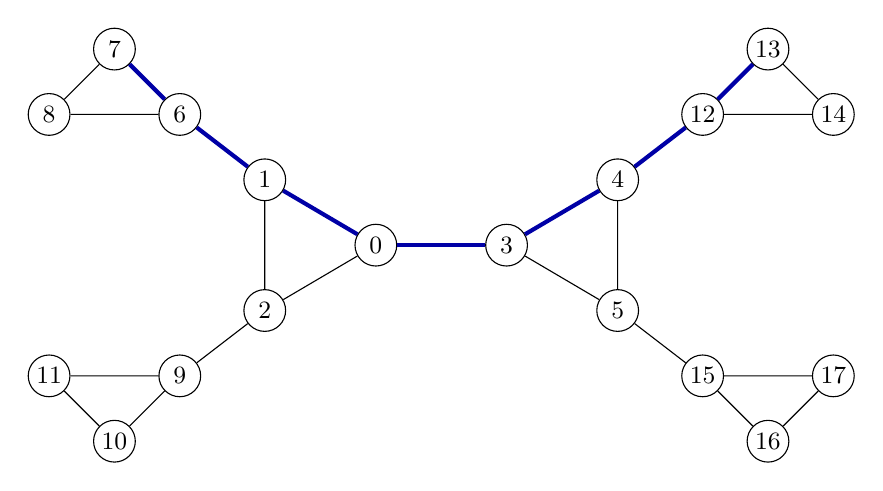
\begin{tikzpicture}[x=0.83cm,y=0.83cm,
 every node/.style={circle,draw,fill=white,inner sep=1pt,minimum size=5.3mm,font=\small}]
\node (0) at (1,0) {0}; \node (1) at (-.7,1) {1}; \node (2) at (-.7,-1) {2};
\node (3) at (3,0) {3}; \node (4) at (4.7,1) {4}; \node (5) at (4.7,-1) {5};
\node (6) at (-2,2) {6}; \node (7) at (-3,3) {7}; \node (8) at (-4,2) {8};
\node (9) at (-2,-2) {9}; \node (10) at (-3,-3) {10}; \node (11) at (-4,-2) {11};
\node (12) at (6,2) {12}; \node (13) at (7,3) {13}; \node (14) at (8,2) {14};
\node (15) at (6,-2) {15}; \node (16) at (7,-3) {16}; \node (17) at (8,-2) {17};
\foreach \a/\b/\c in {0/1/2,3/4/5,6/7/8,9/10/11,12/13/14,15/16/17}
 {\draw (\a)--(\b)--(\c)--(\a);}
\foreach \a/\b in {0/3,1/6,2/9,4/12,5/15} {\draw (\a)--(\b);}
\foreach \a/\b in {7/6,6/1,1/0,0/3,3/4,4/12,12/13}
 {\draw[blue!65!black,line width=1.5pt] (\a)--(\b);}
\end{tikzpicture}
\caption{The eighteen-vertex counterexample. The highlighted path has
eight vertices; no induced tree has more. All edges are specified in
Corollary~\ref{cor:18}.}\label{fig:counter}
\end{figure}

\begin{corollary}[An infinite family]\label{cor:infinite}
The amount by which the right side of \eqref{eq:76} exceeds its left side
is unbounded on connected graphs of maximum degree three.
\end{corollary}
\begin{proof}
Take $H$ to be the complete binary tree of height $h\ge3$, with
$q=2^{h+1}-1$ vertices and diameter $2h$. Its triangle replacement has
\[
\tree(G_H)=4h+2,\qquad
\frac{F_\triangle(G_H)}{\lfloor\overline d(G_H)\rfloor}
=\frac32(2^{h+1}-1).
\]
The difference is positive at $h=3$ and tends to infinity. Its increment
when $h$ increases by one is $3\cdot2^h-4>0$.
\end{proof}

\begin{remark}
No claim is made that eighteen is the smallest possible counterexample
order. The construction gives an exact reduction of an induced-tree
optimization problem to an ordinary tree diameter, rather than merely
a numerical candidate counterexample.
\end{remark}

% Counterexample sections for the expanded manuscript.
% Uses the existing theorem environments, amsmath, amssymb, and TikZ.

\section{WOWII 138: double brooms with a unique maximum independent set}
\label{sec:138}

Write $\operatorname{path}(G)$ for the maximum \emph{number of vertices}
in an induced path of $G$, and let
\[
u(G)=
\begin{cases}
1,&\text{if $G$ has a unique maximum independent set},\\
0,&\text{otherwise}.
\end{cases}
\]
The square $G^2$ has vertex set $V(G)$, with two distinct vertices adjacent
when their distance in $G$ is at most two.  For any graph $H$, put
$M(H)=\{v:\deg_H(v)=\Delta(H)\}$.
For a set $S$ of at least two vertices, the distinct-pair convention is
\[
\operatorname{dist}_{\min,H}(S)
   =\min\{d_H(x,y):x,y\in S,\ x\ne y\}.
\]
The archived statement of WOWII~138 is
\begin{equation}\label{newce:eq:138-source}
\operatorname{path}(G)
   \ge (2+u(G))\operatorname{dist}_{\min}(M(G^2)).
\end{equation}

Two source conventions deserve explicit treatment.  The heading of
definition~74 specifies a \emph{unique maximum independent set}; the body
of that definition accidentally omits ``maximum.''  We use the heading's
meaning.  The notation in \eqref{newce:eq:138-source} also leaves open
whether distances between members of $M(G^2)$ are measured in $G$ or in
$G^2$.  The examples below refute both readings.  Definition~19 does not
explicitly exclude the diagonal $x=y$; we use the nontrivial
distinct-pair reading above.  If the diagonal is included, the minimum
is zero and the printed inequality is tautological, so that reading is
not refuted here.

\begin{proposition}[An infinite counterexample family for 138]
\label{newce:prop:138}
For every integer $k\ge7$, let $B_k$ be the tree obtained from the path
$x_0x_1\cdots x_{2k}$ by adjoining two new leaves at $x_0$ and two new
leaves at $x_{2k}$.  Then
\begin{align}
|V(B_k)|&=2k+5, & |E(B_k)|&=2k+4,\label{newce:eq:138-size}\\
\alpha(B_k)&=k+4, & u(B_k)&=1,\label{newce:eq:138-alpha}\\
M(B_k^2)&=\{x_1,x_{2k-1}\}, &
\operatorname{dist}_{\min,B_k^2}(M(B_k^2))&=k-1,\label{newce:eq:138-square}\\
\operatorname{path}(B_k)&=2k+3.&&\label{newce:eq:138-path}
\end{align}
Consequently the right side of \eqref{newce:eq:138-source}, using the
square metric, is $3k-3>2k+3$.  Using the original metric instead gives
the still larger value $6k-6$.
\end{proposition}

\begin{proof}
Neither $x_0$ nor $x_{2k}$ can belong to a maximum independent set.
Indeed, replacing either such vertex by its two pendant neighbours
increases the set's cardinality by one and preserves independence.
Every maximum independent set therefore contains all four pendant
vertices.  What remains to be chosen is a maximum independent set of
the path $x_1\cdots x_{2k-1}$.

A path on $2k-1$ vertices has a unique independent set of size $k$,
namely its odd-positioned vertices.  To see uniqueness directly, if
$1\le j_1<\cdots<j_k\le2k-1$ are the positions of $k$ pairwise
nonadjacent vertices, then $j_{i+1}\ge j_i+2$.  The available interval
forces $j_1=1$ and every gap to equal two.  Thus the unique maximum
independent set of $B_k$ consists of the four pendant vertices together
with $x_1,x_3,\ldots,x_{2k-1}$, proving
\eqref{newce:eq:138-alpha}.

For a vertex $z$ of a tree $T$, its first and second distance layers are
disjoint and have no repeated vertices, giving
\[
\deg_{T^2}(z)=\sum_{y\in N_T(z)}\deg_T(y).
\]
In $B_k^2$, the vertices $x_1,x_{2k-1}$ consequently have degree five.
Every other backbone vertex has degree four, and each pendant vertex
has degree three.  This proves the description of $M(B_k^2)$.
In any connected graph,
\[
d_{G^2}(a,b)=\left\lceil\frac{d_G(a,b)}2\right\rceil:
\]
one square edge traverses at most two original edges, and a geodesic
in $G$ attains the resulting lower bound by taking steps of length two.
Since $d_{B_k}(x_1,x_{2k-1})=2k-2$, equation
\eqref{newce:eq:138-square} follows.

Every path in a tree is induced.  A longest path in $B_k$ runs from a
pendant vertex at one end of the backbone to a pendant vertex at the
other end.  It has $2k+2$ edges and $2k+3$ vertices, proving
\eqref{newce:eq:138-path}.  Finally,
\[
(2+u(B_k))\operatorname{dist}_{\min,B_k^2}(M(B_k^2))
       -\operatorname{path}(B_k)
   =3(k-1)-(2k+3)=k-6>0.
\]
This proves the counterexample claim for every $k\ge7$.
\end{proof}

\begin{figure}[htbp]
\centering
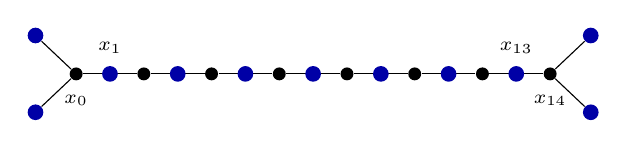
\begin{tikzpicture}[x=0.43cm,y=0.75cm,
  newcespine/.style={circle,fill=black,inner sep=1.65pt},
  newceselected/.style={circle,fill=blue!65!black,inner sep=2pt}]
  \foreach \i in {0,...,14} {
    \node[newcespine] (s\i) at (\i,0) {};
  }
  \foreach \i in {1,...,14} {
    \pgfmathtruncatemacro{\j}{\i-1}
    \draw (s\j)--(s\i);
  }
  \foreach \i in {1,3,5,7,9,11,13} {
    \node[newceselected] at (\i,0) {};
  }
  \node[newceselected] (la) at (-1.2,0.65) {};
  \node[newceselected] (lb) at (-1.2,-0.65) {};
  \node[newceselected] (ra) at (15.2,0.65) {};
  \node[newceselected] (rb) at (15.2,-0.65) {};
  \draw (la)--(s0)--(lb) (ra)--(s14)--(rb);
  \node[below=4pt,font=\scriptsize] at (s0) {$x_0$};
  \node[above=4pt,font=\scriptsize] at (s1) {$x_1$};
  \node[above=4pt,font=\scriptsize] at (s13) {$x_{13}$};
  \node[below=4pt,font=\scriptsize] at (s14) {$x_{14}$};
\end{tikzpicture}
\caption{The nineteen-vertex tree $B_7$.  The eleven blue vertices form
its unique maximum independent set.  Its largest induced path has
seventeen vertices, whereas WOWII~138 requires eighteen under the
square-metric reading.}
\label{newce:fig:138}
\end{figure}

For reproducibility, label the backbone $0,1,\ldots,14$ and add edges
$(0,15)$, $(0,16)$, $(14,17)$, and $(14,18)$.  An exhaustive
maximum-independent-set computation over the $2^{19}=524\,288$ vertex
subsets found independence number eleven and exactly one maximum set,
\[
\{1,3,5,7,9,11,13,15,16,17,18\}.
\]
It also confirmed the square-degree sequence
\[
(4,5,\underbrace{4,\ldots,4}_{11\text{ entries}},5,4,3,3,3,3),
\]
the two maximum-degree square vertices, their distances twelve and six
in $B_7$ and $B_7^2$, respectively, and the diameter sixteen of $B_7$.
These computations supplement the proof; no assertion of minimum
counterexample order is made.

\section{WOWII 256: two hubs with triangle petals}
\label{sec:256}

For a graph without isolated vertices, $\gamma_t(G)$ is the minimum
cardinality of a set $D$ such that every vertex has a neighbour in $D$.
In particular, vertices of $D$ themselves must have neighbours in $D$.
Let
\[
A(G)=\{v:\deg_G(v)=\delta(G)\}
\]
be the minimum-degree set in this section, and retain the open
set-neighbourhood convention
$N(S)=\bigcup_{s\in S}N(s)$.
Thus $N(S)$ may intersect $S$.  In the global edge-neighbourhood
notation,
\[
q_E(G)=\max_{xy\in E(G)}|N(x)\cup N(y)|.
\]
Both $x$ and $y$ belong to $N(x)\cup N(y)$ for every edge $xy$;
neither endpoint is removed.  With these source conventions, WOWII~256
asks for
\begin{equation}\label{newce:eq:256-source}
\gamma_t(G)\ge\frac{2|N(A(G))|}{q_E(G)}.
\end{equation}

\begin{proposition}[An infinite counterexample family for 256]
\label{newce:prop:256}
For an integer $t\ge3$, construct $F_t$ from two hubs $u,v$ and a
central vertex $c$, with edges $uc,cv$.  At each hub attach $t$ triangle
petals: each petal introduces two new vertices $a,b$ and precisely the
three edges $ha,hb,ab$, where $h$ is its hub.  All introduced vertices
are distinct, and there are no further edges.  Then
\begin{align}
|V(F_t)|&=4t+3, & |E(F_t)|&=6t+2,\label{newce:eq:256-size}\\
\gamma_t(F_t)&=3, & |N(A(F_t))|&=4t+2,\label{newce:eq:256-invariants}\\
q_E(F_t)&=2t+3.&&\label{newce:eq:256-q}
\end{align}
The proposed inequality is false for every $t\ge3$.
\end{proposition}

\begin{proof}
There are $4t$ petal vertices in addition to $u,v,c$.  Each of the
$2t$ petals supplies three edges, and the central path supplies two,
proving \eqref{newce:eq:256-size}.
The hubs have degree $2t+1$; every other vertex, including $c$, has
degree two.  Hence
\[
A(F_t)=V(F_t)\setminus\{u,v\}.
\]
Each petal vertex has its petal mate in $A(F_t)$, and both hubs have
neighbours in $A(F_t)$.  In contrast, the only neighbours of $c$ are
$u,v$, neither of which lies in $A(F_t)$.  Consequently
\[
N(A(F_t))=V(F_t)\setminus\{c\},
\qquad |N(A(F_t))|=4t+2.
\]

The set $\{u,c,v\}$ is a total dominating set.  A two-vertex total
dominating set would have to consist of adjacent vertices.  Every
edge is either a central edge, incident with $c$ and one hub, or lies
in a triangle petal at one hub.  In either case, the two endpoints
have no neighbour among the petal vertices at the opposite hub.
Thus the endpoints do not totally dominate those vertices.  No
two-vertex total dominating set exists, so $\gamma_t(F_t)=3$.

The edge-neighbourhood unions can be computed for the three edge
types.  For the central edge $cu$,
\[
N(c)\cup N(u)=\{u,v,c\}\cup
  \{\text{the $2t$ petal vertices at $u$}\},
\]
which has size $2t+3$; the same holds for $cv$.
For a hub-to-petal edge $ua$, with petal mate $b$, the union is
$N(u)\cup\{u\}$, of size $2t+2$.
Finally, for the edge $ab$ inside that petal, the union is
$\{u,a,b\}$, of size three.  Therefore
$q_E(F_t)=2t+3$.

Substitution into \eqref{newce:eq:256-source} would give
\[
3\ge\frac{2(4t+2)}{2t+3}
   =4-\frac8{2t+3}.
\]
The denominator is positive, and the right side minus the left side is
\[
\frac{2t-5}{2t+3}>0\qquad(t\ge3).
\]
Equivalently, clearing denominators would require
$6t+9\ge8t+4$, which is false.  The cleared-denominator deficit
$2t-5$ grows without bound, while the gap in the original inequality
tends to one.
\end{proof}

\begin{figure}[htbp]
\centering
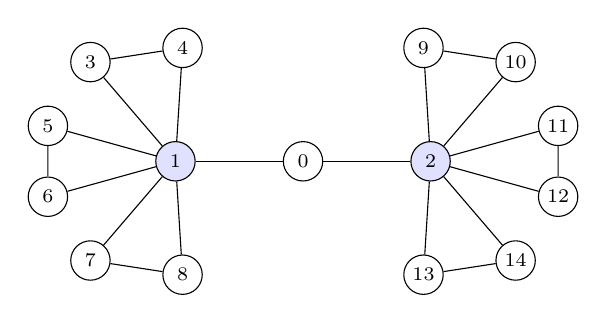
\begin{tikzpicture}[x=0.9cm,y=0.9cm,
  newcevertex/.style={circle,draw,fill=white,inner sep=0pt,
    minimum size=5mm,font=\scriptsize},
  newcehub/.style={newcevertex,fill=blue!12}]
  \node[newcevertex] (c) at (0,0) {$0$};
  \node[newcehub] (u) at (-1.8,0) {$1$};
  \node[newcehub] (v) at (1.8,0) {$2$};
  \node[newcevertex] (a3) at (-3.0,1.4) {$3$};
  \node[newcevertex] (a4) at (-1.7,1.6) {$4$};
  \node[newcevertex] (a5) at (-3.6,0.5) {$5$};
  \node[newcevertex] (a6) at (-3.6,-0.5) {$6$};
  \node[newcevertex] (a7) at (-3.0,-1.4) {$7$};
  \node[newcevertex] (a8) at (-1.7,-1.6) {$8$};
  \node[newcevertex] (a9) at (1.7,1.6) {$9$};
  \node[newcevertex] (a10) at (3.0,1.4) {$10$};
  \node[newcevertex] (a11) at (3.6,0.5) {$11$};
  \node[newcevertex] (a12) at (3.6,-0.5) {$12$};
  \node[newcevertex] (a13) at (1.7,-1.6) {$13$};
  \node[newcevertex] (a14) at (3.0,-1.4) {$14$};
  \draw (u)--(c)--(v);
  \foreach \a/\b in {3/4,5/6,7/8} {
    \draw (u)--(a\a)--(a\b)--(u);
  }
  \foreach \a/\b in {9/10,11/12,13/14} {
    \draw (v)--(a\a)--(a\b)--(v);
  }
\end{tikzpicture}
\caption{The fifteen-vertex counterexample $F_3$ to WOWII~256.
The hubs are $u=1$ and $v=2$, and the central vertex is $c=0$.
Here $\gamma_t=3$, $|N(A)|=14$, and $q_E=9$, so the conjecture would
require $27\ge28$.}
\label{newce:fig:256}
\end{figure}

For the explicit labelling in Figure~\ref{newce:fig:256}, add edges
$01,02$ and the three edges of each petal triangle.  At hub~$1$, use
the pairs $(3,4)$, $(5,6)$, and $(7,8)$.  At hub~$2$, use the pairs
$(9,10)$, $(11,12)$, and $(13,14)$.  There are no other edges.
An independent exhaustive scan of all
$2^{15}-1=32\,767$ nonempty vertex subsets confirmed
$\gamma_t=3$, with witness $\{0,1,2\}$.
Direct computation also confirmed twenty edges, the degree multiset
$\{2^{(13)},7^{(2)}\}$, $|A|=13$, $|N(A)|=14$, and $q_E=9$.
No claim that fifteen is the minimum counterexample order is made.

\section{Total domination and the average distance between centers: WOWII 268}
\label{r4:sec268}

For a connected graph $G$, let
\[
 C(G)=\{v\in V(G):\operatorname{ecc}_G(v)=\operatorname{rad}(G)\}
\]
be its center.  In WOWII~268, the distance average is taken between
distinct vertices of this set, with distances measured in $G$.
Writing $k=|C(G)|$, we use the convention
\begin{equation}
 \label{r4:centeraverage}
 \overline d_C(G)=
 \begin{cases}
 \displaystyle\frac{1}{\binom{k}{2}}
       \sum_{\{u,v\}\subseteq C(G),\,u\ne v}d_G(u,v),&k\ge2,\\[6pt]
 0,&k=1.
 \end{cases}
\end{equation}
The unordered-pair average in \eqref{r4:centeraverage} equals the average
over all ordered pairs of distinct centers.

\begin{theorem}[WOWII 268]
\label{r4:thm268}
Every finite simple connected graph $G$ of order at least two satisfies
\begin{equation}
 \label{r4:268bound}
 \gamma_t(G)\ge
 \left\lfloor 1+\overline d_C(G)\right\rfloor.
\end{equation}
\end{theorem}

We use the classical spanning-tree method for total domination
of DeLaVi\~na, Liu, Pepper, Waller, and West~\cite{DLPWW2007}.
Their radius bound is $\gamma_t(G)\ge\operatorname{rad}(G)$.
The following proof records the additional information needed when
equality holds.

\begin{lemma}
\label{r4:tdtree}
Let $G$ be a finite simple connected graph of order at least two, and let
$D$ be a minimum total dominating set, of size $t$.
There is a spanning tree $T$ of $G$ for which $D$ is a minimum total
dominating set and
\begin{equation}
 \label{r4:tdtreediameter}
 \operatorname{diam}(T)\le 2t-1.
\end{equation}
Consequently $\operatorname{rad}(G)\le t$.
If $\operatorname{rad}(G)=t$, then $G$ has two adjacent center vertices.
\end{lemma}

\begin{proof}
Each component of $G[D]$ has at least two vertices, since every vertex
of $D$ must have a neighbor in $D$.
Choose a spanning tree of each such component, and attach every vertex
of $V(G)\setminus D$ by one edge to a chosen neighbor in $D$.
The resulting graph is a spanning forest whose components correspond
to those of $G[D]$.
Contracting these components in $G$ gives a connected quotient.
Choose edges of $G$ corresponding to a spanning tree of this quotient
and add them to the forest.  The resulting graph $T$ is a spanning tree
in which every vertex still has a neighbor in $D$.
Thus $D$ totally dominates $T$.
Conversely, every total dominating set of $T$ totally dominates $G$,
so $\gamma_t(T)=\gamma_t(G)=t$.

Let $P$ be a diametral path of $T$.
If $d\in D\cap V(P)$, then $d$ has at most two neighbors on $P$.
If $d\in D\setminus V(P)$, it has at most one neighbor on $P$,
since two such neighbors would create a cycle in $T$.
Every vertex of $P$ has a neighbor in $D$, hence
\[
 |V(P)|
 \le \sum_{d\in D}|N_T(d)\cap V(P)|
 \le 2|D|=2t.
\]
This proves \eqref{r4:tdtreediameter}.
Using the radius--diameter formula for a tree gives
\begin{equation}
 \label{r4:radiuschain}
 \operatorname{rad}(G)
 \le\operatorname{rad}(T)
 =\left\lceil\frac{\operatorname{diam}(T)}2\right\rceil
 \le t.
\end{equation}

Now suppose $\operatorname{rad}(G)=t$.
Equality must hold throughout \eqref{r4:radiuschain}, and
\eqref{r4:tdtreediameter} then forces
$\operatorname{diam}(T)=2t-1$.
The center of this odd-diameter tree consists of two adjacent vertices,
say $x$ and $y$, both with eccentricity $t$ in $T$.
Since adding edges cannot increase distances,
\[
 \operatorname{ecc}_G(x)\le\operatorname{ecc}_T(x)=t
 =\operatorname{rad}(G),
\]
so $x$ is a center of $G$; the same argument applies to $y$.
Their edge in $T$ is also an edge in $G$.
\end{proof}

\begin{proof}[Proof of Theorem~\ref{r4:thm268}]
Put $t=\gamma_t(G)$ and $r=\operatorname{rad}(G)$.
If $|C(G)|=1$, the right-hand side of \eqref{r4:268bound} is $1$,
whereas $t\ge2$.
We may therefore assume that $|C(G)|\ge2$.
Every pair of centers is at distance at most $r$, so
$\overline d_C(G)\le r$.
Lemma~\ref{r4:tdtree} gives $t\ge r$.
If $t>r$, integrality yields
\[
 \left\lfloor1+\overline d_C(G)\right\rfloor
 \le r+1\le t.
\]

It remains to consider $t=r$.
Since a total dominating set has at least two vertices, $r\ge2$.
By Lemma~\ref{r4:tdtree}, two centers of $G$ are adjacent.
Their distance is $1<r$, while every other distinct center pair has
distance at most $r$.
The average is therefore strictly smaller than $r$:
\[
 \overline d_C(G)<r.
\]
Since $r$ is an integer, this implies
$\lfloor1+\overline d_C(G)\rfloor\le r=t$, as required.
\end{proof}

\begin{remark}[Domain and computational check]
\label{r4:268check}
The order restriction excludes $K_1$, which has no total dominating set.
An exact exhaustive check of all $1{,}893{,}731$ connected labeled graphs
on two through seven vertices found no failure of
\eqref{r4:268bound}, the radius bound, or the adjacent-center conclusion
in the equality case of Lemma~\ref{r4:tdtree}.
This computation is a secondary check; the proof above is independent
of it.
\end{remark}

\begin{remark}[The ceiling variant]
\label{r4:269open}
WOWII~269 replaces the floor in \eqref{r4:268bound} by a ceiling under
the additional assumption that $G$ contains no $4$-cycle.
The strict inequality $\overline d_C(G)<r$ used above does not establish
that stronger assertion.  No resolution of WOWII~269 is claimed here.
\end{remark}


% Complete counterexample sections for WOWII 369 and 392c.
% Requires only the main document's theorem/proof/remark environments,
% amsmath/amssymb, and bibliography key WOWII. All labels use r4:.

\section{Conjecture 369: a first-zero Havel--Hakimi counterexample}
\label{r4:sec369}

For a graph $G$, let $\gamma_t(G)$ denote its total domination number:
every vertex, including each selected vertex, must have a neighbour in the
selected set.  Let $\operatorname{dd}_{\mathrm{mode}}(G)$ be the number of
distinct degree values whose frequencies are largest.  Define $k(G)$ by
the following Havel--Hakimi procedure.  Sort the degree sequence in
nonincreasing order, remove its largest entry $a$, subtract one from each
of the next $a$ entries, and sort again.  Then $k(G)$ is the number of
reductions up to and including the first reduction whose resulting
sequence contains a zero.  This is the first-zero convention in source
Definition~110; it is not the number of reductions required to make every
entry zero.

Conjecture~369 of \cite{WOWII}, dated February~18, 2009, asserts that every
tree $T$ of order $n>2$ satisfies
\begin{equation}
  \gamma_t(T)\ge
  \operatorname{dd}_{\mathrm{mode}}(T)+(n\bmod 2)\,k(T).
  \label{r4:369-assertion}
\end{equation}
The following counterexample has a unique degree mode and odd order, so
neither a modal tie nor the parity factor obscures the failure.

\begin{theorem}[A 29-vertex counterexample to Conjecture 369]
\label{r4:369-finite}
There is a tree $T$ with
\[
  |V(T)|=29,\qquad
  \gamma_t(T)=6,\qquad
  \operatorname{dd}_{\mathrm{mode}}(T)=1,\qquad
  k(T)=6.
\]
Consequently, the two sides of \eqref{r4:369-assertion} are $6$ and $7$,
respectively.
\end{theorem}

\begin{proof}
Start with the nine-vertex path whose vertices, in order, are
\[
  (s_0,s_1,a,s_2,s_3,b,c,s_4,s_5).
\]
Attach four new leaves to each of $s_0,s_5$, and three new leaves to each
of $s_1,s_2,s_3,s_4$.  No other edges or vertices are added.  The resulting
graph is a tree with twenty leaves and degree multiset
\[
  (5^6,2^3,1^{20}),
\]
where superscripts indicate multiplicities.  Thus it has $29$ vertices,
and degree one is its unique most frequent degree.  In particular,
$\operatorname{dd}_{\mathrm{mode}}(T)=1$.

Each $s_i$ is the neighbour of a leaf, so every total dominating set must
contain all six vertices $s_i$.  Conversely,
$D=\{s_0,s_1,\ldots,s_5\}$ totally dominates the tree.  The three edges
$s_0s_1,s_2s_3,s_4s_5$ dominate the selected vertices themselves; each leaf
has its support in $D$; and $a,b,c$ are adjacent to $D$.  Hence
$\gamma_t(T)=6$.

The complete Havel--Hakimi trace through its first zero is
\begin{equation}
\begin{array}{c|l}
  \text{Number of reductions} & \text{Resulting degree multiset}\\ \hline
  0 & 5^6,\ 2^3,\ 1^{20}\\
  1 & 4^5,\ 2^3,\ 1^{20}\\
  2 & 3^4,\ 2^3,\ 1^{20}\\
  3 & 2^6,\ 1^{20}\\
  4 & 2^3,\ 1^{22}\\
  5 & 1^{24}\\
  6 & 1^{22},\ 0
\end{array}
\label{r4:369-trace}
\end{equation}
All entries remain positive through the fifth reduction, and the sixth
creates a zero.  Therefore $k(T)=6$.  Since $29$ is odd, the conjecture
would require $6\ge 1+6=7$, which is false.
\end{proof}

\begin{remark}[Explicit labelling]
\label{r4:369-labelling}
An edge-list certificate is obtained by setting $s_i=i$ for $0\le i\le5$
and $(a,b,c)=(6,7,8)$.  The eight core edges are
\[
\begin{gathered}
  (0,1),\ (2,3),\ (4,5),\ (1,6),\ (6,2),\\
  (3,7),\ (7,8),\ (8,4).
\end{gathered}
\]
Attach vertices $9,\ldots,12$ to $0$, $13,\ldots,15$ to $1$,
$16,\ldots,18$ to $2$, $19,\ldots,21$ to $3$,
$22,\ldots,24$ to $4$, and $25,\ldots,28$ to $5$.
No claim that this counterexample has minimum possible order is needed.
\end{remark}

\begin{theorem}[An unbounded family for Conjecture 369]
\label{r4:369-family}
For each integer $r\ge3$ with $r\equiv3\pmod6$, there is a tree $T_r$
such that
\begin{align*}
  |V(T_r)|&=4r^2-3r+2, & \gamma_t(T_r)&=2r,\\
  \operatorname{dd}_{\mathrm{mode}}(T_r)&=1,
  &k(T_r)&=2r-1+\frac r3.
\end{align*}
The right-hand side of \eqref{r4:369-assertion} exceeds its left-hand side
by $r/3$.
\end{theorem}

\begin{proof}
Begin with $r$ disjoint edges and let $D$ be the set of their $2r$
endpoints.  Arrange these edges as consecutive blocks of a chain.  Join
consecutive blocks by internally disjoint paths, using different
endpoints of each intermediate block.  Use one joining path of length
three and $r-2$ joining paths of length two.  Their internal vertices are
all new.  There are exactly $2+(r-2)=r$ such vertices, and the resulting
core is a path on $3r$ vertices, with both endpoints in $D$.

Attach leaves to every vertex of $D$ until each has degree $2r-1$.
The sum of the core degrees of vertices in $D$ is
$2r+2(r-1)=4r-2$.  The number of added leaves is therefore
\begin{equation}
  \ell=2r(2r-1)-(4r-2)=4r^2-6r+2.
  \label{r4:369-leaves}
\end{equation}
The resulting tree has order $2r+r+\ell=4r^2-3r+2$ and degree multiset
\begin{equation}
  \bigl((2r-1)^{2r},\ 2^r,\ 1^\ell\bigr).
  \label{r4:369-degree-sequence}
\end{equation}
Its order is odd because $r$ is odd.  Moreover, $\ell>2r\ge r$, so degree
one is the unique mode.

Every vertex in $D$ has at least $(2r-1)-2=2r-3$ pendant neighbours and is
therefore forced into every total dominating set.  The set $D$ itself
totally dominates the tree: its vertices have their original partners
in $D$, every leaf has its support in $D$, and each internal vertex of
every joining path is adjacent to an endpoint in $D$.  This proves
$\gamma_t(T_r)=2r$.

It remains to compute the first-zero step, rather than merely bound it.
Put $t=2r$.  After $j$ Havel--Hakimi reductions, for
$0\le j\le t-3$, the sequence is
\begin{equation}
  \bigl((t-1-j)^{t-j},\ 2^r,\ 1^\ell\bigr),
  \label{r4:369-high-phase}
\end{equation}
with equal degree-two groups combined when $j=t-3$.
Indeed, whenever the leading degree is at least three, it equals the
number of other entries in its leading group.  A reduction removes one
leading entry and decreases every other entry in that group by one,
leaving the original degree-two entries and the ones unchanged.  This
proves \eqref{r4:369-high-phase} by induction, and no zero occurs during
these reductions.

After $t-3$ reductions, the sequence is $(2^{r+3},1^\ell)$.
Because $r+3$ is divisible by three, exactly $(r+3)/3$ further reductions
remove all the twos: each reduction removes one two and changes two
other twos into ones.  None creates a zero.  The resulting sequence
consists of $\ell+2(r+3)/3$ ones, a positive even number.  The next
reduction removes a one and changes another one into zero.  Consequently,
\[
  k(T_r)=(t-3)+\frac{r+3}{3}+1
        =2r-1+\frac r3.
\]
Since $|V(T_r)|$ is odd and the degree mode is unique, the asserted lower
bound is $1+k(T_r)=2r+r/3$, whereas the actual total domination number is
$2r$.  The deficit is therefore $r/3$, which is unbounded.
For $r=3$ this construction gives the 29-vertex tree in
Theorem~\ref{r4:369-finite}.
\end{proof}

\section{Conjecture 392c: nonadjacent ports in a cycle necklace}
\label{r4:sec392c}

A set $D\subseteq V(G)$ is a \emph{2-dominating set} if every vertex
outside $D$ has at least two neighbours in $D$; selected vertices have no
additional requirement.  Write $\gamma_2(G)$ for its minimum size and
$\mu(G)$ for the matching number.  Let
\[
  A_\delta=\{v\in V(G):\deg_G(v)=\delta(G)\},
\]
and let $c_{\mathrm{cut}}(G)$ denote the \emph{number of cut vertices}, not vertex
connectivity.  Conjecture~392c of \cite{WOWII}, dated January~2010,
asserts, for every connected graph of order greater than two,
\begin{equation}
  \gamma_2(G)\le
  \mu\bigl(G[V(G)\setminus A_\delta]\bigr)
  +|A_\delta|+c_{\mathrm{cut}}(G).
  \label{r4:392c-assertion}
\end{equation}

\begin{lemma}[A five-cycle with two nonadjacent ports]
\label{r4:392c-local}
Suppose a graph contains an induced cycle
$x_0x_1x_2x_3x_4x_0$ and only $x_0,x_2$ may have neighbours outside this
cycle.  Every 2-dominating set contains at least three vertices of the
cycle.
\end{lemma}

\begin{proof}
Let $D$ be a 2-dominating set.  If $x_1\notin D$, both $x_0,x_2$ must
belong to $D$, since they are the only neighbours of $x_1$.  If these
were the only selected cycle vertices, each of $x_3,x_4$ would have only
one selected neighbour.  A third selected vertex is therefore necessary.

If $x_1\in D$ and the cycle contained at most two selected vertices,
at most one of $x_0,x_2,x_3,x_4$ could be selected.  At least one of
$x_3,x_4$ must be selected: if both were omitted, each would have at most
one selected neighbour.  But selecting just one of $x_3,x_4$ leaves the
other with only that one selected neighbour, since neither port is then
selected.  This is again impossible.
\end{proof}

\begin{theorem}[An unbounded family for Conjecture 392c]
\label{r4:392c-family}
For every integer $k\ge3$ there is a connected graph $G_k$ satisfying
\begin{align*}
  |V(G_k)|&=5k+1, & |E(G_k)|&=6k+1,\\
  \gamma_2(G_k)&=3k+1, & |A_\delta|&=1,\\
  \mu\bigl(G_k[V(G_k)\setminus A_\delta]\bigr)
    &=\left\lfloor\frac{5k}{2}\right\rfloor,
  &c_{\mathrm{cut}}(G_k)&=1.
\end{align*}
Thus the left-hand side of \eqref{r4:392c-assertion} exceeds its
right-hand side by $\lceil k/2\rceil-1$.
\end{theorem}

\begin{proof}
Take $k$ vertex-disjoint five-cycles $C_i$, with vertices
$x_{i,0},x_{i,1},\ldots,x_{i,4}$ in cyclic order, where block indices are
taken modulo $k$.  Add the joining edges
\begin{equation}
  x_{i,2}x_{i+1,0}\qquad(0\le i<k).
  \label{r4:392c-joining-edges}
\end{equation}
Call this graph $H_k$.  Finally, add one new vertex $z$ adjacent only to
$x_{0,0}$, obtaining $G_k$.  Its order and size are $5k+1$ and $6k+1$.
The two ports in each five-cycle, numbered $0$ and $2$, are nonadjacent;
this placement is essential to the local obstruction.

By Lemma~\ref{r4:392c-local}, every 2-dominating set contains at least
three vertices of each block.  The leaf $z$ must also be selected,
because a vertex of degree one cannot have two selected neighbours.
Hence $\gamma_2(G_k)\ge3k+1$.  Conversely, the set
\begin{equation}
  D=\{z\}\cup
    \bigcup_{i=0}^{k-1}\{x_{i,1},x_{i,3},x_{i,4}\}
  \label{r4:392c-witness}
\end{equation}
is 2-dominating: each omitted port has both its cycle neighbours in
$D$.  Therefore $\gamma_2(G_k)=3k+1$.

The vertex $z$ is the unique leaf.  The nonport cycle vertices have
degree two, the ports other than $x_{0,0}$ have degree three, and
$x_{0,0}$ has degree four.  It follows that $A_\delta=\{z\}$ and
$G_k[V(G_k)\setminus A_\delta]=H_k$.

We next verify the cut-vertex count.  The paths
$x_{i,0}x_{i,1}x_{i,2}$ together with the joining edges form a cycle
through all three of these vertices in every block.  The remaining
vertices form, for each block, the additional path
$x_{i,0}x_{i,4}x_{i,3}x_{i,2}$.  Deleting a vertex of the first cycle
leaves a connected path, and every additional path retains at least
one endpoint on it.  Deleting an internal vertex of an additional path
leaves its remaining pieces attached to the intact first cycle.
Thus deleting any single vertex of $H_k$ leaves a connected graph.
Adding the pendant vertex $z$ creates exactly one cut vertex,
$x_{0,0}$.  Hence $c_{\mathrm{cut}}(G_k)=1$.

The order bound gives $\mu(H_k)\le\lfloor5k/2\rfloor$.  To attain it,
pair blocks $0,1$, then $2,3$, and so on, and select the joining edge
between the two blocks of each pair.  In each paired block, deleting
the endpoint of that selected joining edge leaves a four-vertex path;
select its two-edge perfect matching.  Each pair of blocks contributes
five matching edges.  If $k$ is odd, choose two disjoint cycle edges
in the remaining block.  The resulting matching has
\[
  5\left\lfloor\frac k2\right\rfloor+2(k\bmod2)
  =\left\lfloor\frac{5k}{2}\right\rfloor
\]
edges, proving equality.

The proposed upper bound is therefore $\lfloor5k/2\rfloor+2$, while
the actual 2-domination number is $3k+1$.  Their difference is
\[
  3k+1-\left(\left\lfloor\frac{5k}{2}\right\rfloor+2\right)
  =\left\lceil\frac k2\right\rceil-1>0
  \qquad(k\ge3).
\]
The difference tends to infinity with $k$.
\end{proof}

\begin{remark}[The explicit 16-vertex member]
\label{r4:392c-finite}
For $k=3$, the vertex set is
$\{z\}\cup\{x_{i,j}:0\le i\le2,\ 0\le j\le4\}$.
In addition to the three five-cycle edge sets, add exactly
\[
  x_{0,2}x_{1,0},\qquad x_{1,2}x_{2,0},\qquad
  x_{2,2}x_{0,0},\qquad zx_{0,0}.
\]
This gives a completely specified graph with $16$ vertices and $19$
edges.  The displayed set \eqref{r4:392c-witness} has ten vertices,
and the block obstruction plus the forced leaf proves its optimality.
The other invariants are $\mu(H_3)=7$, $|A_\delta|=1$, and
$c_{\mathrm{cut}}(G_3)=1$.  Thus \eqref{r4:392c-assertion} would require
$10\le7+1+1=9$.  No minimum-order claim is made.
\end{remark}


% Integration snippet: WOWII 305, 393d, and 400c.
% Uses amsmath/amssymb and the theorem, lemma, proposition, proof, remark
% environments already supplied by the main document. All labels start r5:.

\subsection{Shared-hub variants of the WOWII392c counterexample}
\label{r7:392c}

The supplied notes give a second construction for the already refuted
statement 392c. Sharing two hubs between the pentagons reduces the
matching number more than in the earlier necklace. Identifying those
hubs gives a further variant. Both families are recorded below; the
earlier 16-vertex necklace remains the smaller first counterexample.

\begin{proposition}\label{r7:family392c}
For $k\ge4$, there is a connected graph $F_k$ of order $5k+3$ with
\[
 \gamma_2(F_k)=3k+1,
 \qquad \mu(F_k-A_\delta)+|A_\delta|+\kappa_v(F_k)=2k+4.
\]
There is also, for $k\ge3$, a connected graph $F'_k$ of order $5k+2$
with
\[
 \gamma_2(F'_k)=3k+1,
 \qquad \mu(F'_k-A_\delta)+|A_\delta|+\kappa_v(F'_k)=2k+3.
\]
The symbol $\kappa_v$ denotes the number of cut vertices, as in the
source statement, rather than vertex connectivity.
\end{proposition}
\begin{proof}
Start with $k$ disjoint pentagons, whose vertices in cyclic order are
$c_{i,0},\ldots,c_{i,4}$. For $F_k$, add two hubs $s_1,s_2$, join
$s_1$ to every $c_{i,0}$ and $s_2$ to every $c_{i,2}$, and attach one
pendant vertex $p$ to $s_1$. For $F'_k$, use one hub $s$ adjacent to
both $c_{i,0}$ and $c_{i,2}$ in every pentagon, and attach $p$ to $s$.

In either construction, each pentagon contributes at least three
vertices to any 2-dominating set. Indeed, if $c_{i,1}$ is omitted,
then $c_{i,0},c_{i,2}$ must both be chosen, and these two alone do not
2-dominate $c_{i,3}$. If $c_{i,1}$ is chosen, a set containing only
one further pentagon vertex cannot 2-dominate both $c_{i,3}$ and
$c_{i,4}$: if one of them is chosen, the other still needs its
neighboring port; if neither is chosen, their required neighbors
already exceed the remaining allowance. The pendant vertex is also
forced. Thus $\gamma_2\ge3k+1$. Choosing $p$ and
$c_{i,0},c_{i,2},c_{i,3}$ from every pentagon attains this bound.
Both hubs in $F_k$ have enough chosen neighbors because $k\ge2$.

The pendant vertex is the unique minimum-degree vertex. In $F_k-p$,
a matching uses at most two hub edges and at most two internal edges
per pentagon, hence has size at most $2k+2$. Equality is attained by
matching the two hubs into different pentagons, taking a perfect
matching in the remaining four-vertex path of each such pentagon,
and two edges from every other pentagon. Likewise
$\mu(F'_k-p)=2k+1$: use one hub edge, a perfect matching in the
remaining four vertices of that pentagon, and two edges from each
other pentagon.

The only cut vertex of $F_k$ is $s_1$. After deleting a hub, each
pentagon remains attached to the other hub; after deleting a
pentagon vertex, its remaining path is attached to at least one
hub, and another intact pentagon still connects the two hubs.
Thus the core has no cut vertex, whereas deleting $s_1$ separates
$p$. In $F'_k$, deleting any pentagon vertex leaves that pentagon
attached to $s$ through at least one surviving port. The hub $s$ is
the sole cut vertex. Substituting $|A_\delta|=\kappa_v=1$ gives the
two formulas, with deficits $k-3$ and $k-2$, respectively.
\end{proof}

The supplied $F_4$ has 23 vertices and 29 edges, with $13>12$.
The derived $F'_3$ has 17 vertices and 22 edges, with $10>9$.
The standalone verifier checks their supplied or explicitly constructed
adjacency data and considers all $2^{23}$ and $2^{17}$ subsets,
respectively, for exact 2-domination.

\section{Complement-edge compression and statement 305}
\label{r5:sec305}

For a connected noncomplete graph \(G\), put
\[
q=\max_{uv\in E(\overline G)}
   \bigl|N_{\overline G}(u)\cup N_{\overline G}(v)\bigr|.
\]
The neighbourhoods are open. In particular, both endpoints of the
complement edge \(uv\) belong to the displayed union. Statement 305
of the catalogue \cite{WOWII} asserts
\begin{equation}\label{r5:eq305}
\gamma_t(G)\le \left\lceil\frac{2q}{3}\right\rceil
\end{equation}
for connected graphs of order greater than two. We first isolate the
compression that proves the assertion on its defined domain.

\begin{lemma}[Complement-edge compression]\label{r5:compression}
Let \(G\) be connected and noncomplete, let \(H=\overline G\), and choose
\(uv\in E(H)\) with
\[
S=N_H(u)\cup N_H(v),\qquad |S|=q.
\]
If \(q<|V(G)|\), there is a connected subgraph \(J\) of \(G\), with
\(q+1\) vertices, such that every total dominating set of \(J\) is a
total dominating set of \(G\).
\end{lemma}
\begin{proof}
The vertices \(u,v\) belong to \(S\). Consider a component \(C\) of
\(G[S]\) that does not contain both \(u\) and \(v\), and choose
\(a\in\{u,v\}\setminus C\). For each \(x\in C\), the vertices \(a,x\)
lie in different components of \(G[S]\). Consequently \(ax\in E(H)\)
and
\[
C\subseteq N_H(a),\qquad S\setminus C\subseteq N_H(x).
\]
Thus \(S\subseteq N_H(a)\cup N_H(x)\). Since \(q\) is the maximum
complement-edge neighbourhood size, this union has at most \(|S|\)
vertices, and hence equals \(S\). In particular, \(N_H(x)\subseteq S\).
Every vertex of \(C\) is therefore adjacent in \(G\) to every vertex
outside \(S\).

The same conclusion holds for \(u,v\), directly from the definition
of \(S\). Let \(U\) consist of \(u,v\) and all vertices in components
of \(G[S]\) that do not contain both endpoints. Every component of
\(G[S]\) meets \(U\), and every vertex of \(U\) is adjacent in \(G\)
to every vertex outside \(S\).

Choose \(w\notin S\). Define \(J\) on \(S\cup\{w\}\) by taking all
edges of \(G[S]\), together with the edges \(wx\) for \(x\in U\).
These are edges of \(G\), and \(J\) is connected because every
component of \(G[S]\) meets \(U\).

If \(D\) totally dominates \(J\), domination of \(w\) forces
\(D\cap U\ne\varnothing\). Any vertex in this intersection dominates
every vertex of \(V(G)\setminus S\). The vertices of \(S\) are already
totally dominated in \(J\), so \(D\) totally dominates \(G\).
\end{proof}

For clarity, we record the classical total-domination estimate used
below. This is the theorem of Cockayne, Dawes, and Hedetniemi
\cite{CDH1980}; see also \cite[Theorem~1]{HH2009}. The proof included
here is an elementary reproof of that known result.

\begin{lemma}[Classical total-domination bound]\label{r5:classicalTD}
Every connected graph \(F\) of order \(t\ge3\) satisfies
\[
\gamma_t(F)\le \left\lfloor\frac{2t}{3}\right\rfloor.
\]
\end{lemma}
\begin{proof}
It suffices to prove the assertion for a spanning tree, since a total
dominating set of a spanning tree also totally dominates the original
graph. We prove the real-valued bound \(2t/3\) for trees by induction.
Root a tree \(T\) of order \(t\ge3\) at a leaf, and let its maximum
depth be \(h\ge2\).

Suppose first that some vertex \(y\) at depth \(h-1\) has
\(a\ge2\) leaf children. Let \(z\) be its parent. Remove \(y\) and
its \(a\) children, leaving a tree \(T'\) of order
\(r=t-a-1\ge1\). If \(r\ge3\), a total dominating set of \(T'\),
together with \(y,z\), totally dominates \(T\) and has size at most
\[
\frac{2r}{3}+2\le\frac{2t}{3}.
\]
If \(r=1\) or \(r=2\), the pair \(\{y,z\}\) totally dominates \(T\);
here \(t\ge4\), so the same bound holds.

We may therefore assume that every vertex at depth \(h-1\) that has
children has exactly one leaf child. Choose a grandparent \(z\) of
a deepest leaf. Its descendant subtree consists of \(z\), of
\(k\ge1\) children each having one leaf child, and of \(\ell\ge0\)
children that are themselves leaves. The subtree has
\(s=1+2k+\ell\) vertices. Let \(D_z\) consist of \(z\) and those
\(k\) support children. It totally dominates the subtree and
satisfies
\[
3|D_z|=3(k+1)\le2(1+2k+\ell)=2s,
\]
because \(k+2\ell\ge1\).

Delete this subtree. If the remaining tree has order \(r\ge3\),
combine its inductively obtained total dominating set with \(D_z\).
If \(r=0\), use \(D_z\) alone. If \(r=1\), the remaining vertex is
the parent of \(z\) and is dominated by \(z\), so \(D_z\) again
suffices. Finally, if \(r=2\), let \(w\) be the parent of \(z\).
The remaining tree is the edge from \(w\) to the root. Add \(w\)
to \(D_z\); the resulting set totally dominates \(T\) and has size
\[
k+2\le \frac{2(3+2k+\ell)}{3}=\frac{2t}{3}.
\]
This completes the induction. Integer-valuedness gives the floor.
\end{proof}

\begin{theorem}[WOWII 305 on its defined domain]\label{r5:thm305}
Every connected noncomplete graph \(G\) of order greater than two
satisfies \eqref{r5:eq305}.
\end{theorem}
\begin{proof}
If \(q=|V(G)|\), Lemma~\ref{r5:classicalTD} gives
\[
\gamma_t(G)\le\left\lfloor\frac{2q}{3}\right\rfloor
             \le\left\lceil\frac{2q}{3}\right\rceil.
\]
Otherwise apply Lemma~\ref{r5:compression}. Its graph \(J\) has
order \(q+1\ge3\), because the two endpoints of a complement edge
belong to its neighbourhood union. Therefore
\[
\gamma_t(G)\le\gamma_t(J)
 \le\left\lfloor\frac{2(q+1)}{3}\right\rfloor
 =\left\lceil\frac{2q}{3}\right\rceil.
\]
The last equality follows by considering \(q\) modulo three.
\end{proof}

\begin{remark}[Complete graphs and the empty maximum]\label{r5:305domain}
For a complete graph the original maximum ranges over an empty edge
set and has no real value. The theorem proves the full nonempty-maximum
domain without silently imposing a convention. An everywhere-defined
extension is obtained by replacing \(q\) with
\[
q^*(G)=\max\!\left(
\{2\}\cup
\bigl\{|N_{\overline G}(u)\cup N_{\overline G}(v)|:
                         uv\in E(\overline G)\bigr\}\right).
\]
For complete graphs this gives the correct bound
\(\gamma_t(G)=2=\lceil2q^*(G)/3\rceil\).
\end{remark}

\paragraph{Finite verification.}
An exact check covered all \(27\,470\) noncomplete connected labelled
graphs of orders three through six. For the \(11\,318\) cases with
\(q<|V(G)|\), it constructed \(J\) and checked the transfer property
for every total dominating set of \(J\), a total of \(242\,241\) sets.
These computations support the proof and are not premises of it.

\section{A corona counterexample family for statement 393d}
\label{r5:sec393d}

A set \(D\subseteq V(G)\) is \emph{2-dominating} if every vertex
outside \(D\) has at least two neighbours in \(D\); its minimum
cardinality is \(\gamma_2(G)\). This condition places no requirement
on vertices already in \(D\). Let \(P(G)\) be the pendant-vertex set,
let \(M(G)\) be the maximum-degree vertex set, and define
\[
\nu_4(v)=|\{Q\subseteq V(G): |Q|=4,\ G[Q]\cong K_4,\ v\in Q\}|,
\qquad
M_4(G)=\{v:\nu_4(v)=\max_x\nu_4(x)\}.
\]
The original 393d statement \cite{WOWII} proposes
\begin{equation}\label{r5:eq393d}
\gamma_2(G)\le
\mu\!\left(G[V(G)\setminus N_G(N_G(P(G)))]\right)
+\alpha\!\left(G[V(G)\setminus M(G)]\right)+|M_4(G)|.
\end{equation}
The source's Symbol-font \(\alpha\) denotes independence, and \(M_4\)
counts vertices attaining the maximum number of incident copies of
\(K_4\). Both neighbourhood operations in \eqref{r5:eq393d} are open.

\begin{lemma}[Corona identities]\label{r5:corona}
Let \(H\) be connected of order \(h\ge2\), and let \(G=H\circ K_1\)
be obtained by adjoining one private leaf to every vertex of \(H\).
Then
\begin{align}
\gamma_2(G)&=h+\gamma(H),\label{r5:corona2dom}\\
N_G(N_G(P(G)))&=V(G),\label{r5:coronaN}\\
\alpha\!\left(G[V(G)\setminus M(G)]\right)&=h.\label{r5:coronaalpha}
\end{align}
Moreover, the copies of \(K_4\) in \(G\) are exactly those in \(H\).
\end{lemma}
\begin{proof}
Every new leaf must belong to every 2-dominating set. Once these
\(h\) leaves are selected, a core vertex \(v\in V(H)\) that is not
selected has one selected neighbour, its own leaf. It has a second
precisely when it has a selected neighbour in \(H\). Thus the selected
core vertices must form an ordinary dominating set of \(H\), and
every such set suffices. This proves \eqref{r5:corona2dom}.

Since \(H\) has no isolated vertices, its vertices have degree at
least two in \(G\). Hence \(P(G)\) consists exactly of the new
leaves, and \(N_G(P(G))=V(H)\). Every leaf has a neighbour in \(H\),
and every vertex of \(H\) has a neighbour in \(H\), proving
\eqref{r5:coronaN}.

All maximum-degree vertices of \(G\) lie in \(H\). Deleting them
leaves the \(h\) new leaves as an independent set. Conversely, each
of the \(h\) pairs consisting of a core vertex and its private leaf
contributes at most one vertex to any independent set. These pairs
still partition the remaining vertices into sets of size one or
two after the deletion. This proves \eqref{r5:coronaalpha}.
Finally, a pendant vertex belongs to no \(K_4\).
\end{proof}

\begin{theorem}[An unbounded deficit in 393d]\label{r5:thm393d}
For every integer \(r\ge1\), there is a connected graph \(G_r\) of
order \(16+4r\) for which the left-hand side of
\eqref{r5:eq393d} is \(12+3r\), while its right-hand side is
\(12+2r\).
\end{theorem}
\begin{proof}
Start with a \(K_4\) on \(a_0,a_1,a_2,a_3\). Give each \(a_i\)
one private leaf \(b_i\), and attach \(r\) further, mutually
vertex-disjoint paths
\[
a_0u_jv_j,\qquad 1\le j\le r,
\]
whose only vertex in the preceding graph is \(a_0\). Call the
resulting graph \(H_r\). It has \(h=8+2r\) vertices and
\(10+2r\) edges. Its only copy of \(K_4\) is the displayed clique.

Every dominating set of \(H_r\) meets each pair \(\{a_i,b_i\}\),
because \(b_i\) has no other neighbour, and meets each pair
\(\{u_j,v_j\}\), because \(v_j\) has no other neighbour. These
\(4+r\) pairs are disjoint. Conversely, all four \(a_i\), together
with the \(r\) vertices \(u_j\), form a dominating set. Therefore
\[
\gamma(H_r)=4+r.
\]

Set \(G_r=H_r\circ K_1\). Lemma~\ref{r5:corona} gives
\[
\gamma_2(G_r)=(8+2r)+(4+r)=12+3r.
\]
The matching term in \eqref{r5:eq393d} is zero because its induced
vertex set is empty. The independence term is \(8+2r\).
Exactly the four clique vertices have positive \(K_4\)-incidence,
and each lies in one copy, so \(|M_4(G_r)|=4\). The proposed
right-hand side is consequently \(12+2r\), smaller by exactly \(r\).
\end{proof}

The first member has \(20\) vertices and \(22\) edges, with
\(\gamma_2=15\) and proposed upper bound \(14\). The family has
an unbounded additive deficit; no assertion of minimum counterexample
order is made.

\paragraph{Finite verification.}
The construction was checked for \(r=1,2,3\). For \(r=1\), the
verifier considered all \(2^{20}=1\,048\,576\) vertex subsets,
discarding sets that omit a forced leaf before testing 2-domination.
For \(r=2,3\), it checked all supersets of the forced leaves:
\(4\,096\) and \(16\,384\) sets, respectively. Independent checks
of ordinary domination in \(H_r\), the independence term,
double open neighbourhoods, and all \(K_4\) copies agreed with the
formulas above.

\subsection{A smaller supplied counterexample to WOWII393d}
\label{r7:393d}

The supplied research notes give a 16-vertex counterexample, smaller than
the earlier 20-vertex example. The following extension retains its
construction and gives another family with unbounded deficit. This is
an additional certificate for the already refuted statement 393d.

\begin{proposition}\label{r7:family393d}
For every integer $r\ge2$, there is a connected graph $J_r$ of order
$6r+4$ such that
\[
 \gamma_2(J_r)=4r+1,
 \qquad
 \mu(J_r[V\setminus N(N(P))])+\alpha(J_r[V\setminus M])+|M_4|
 =2r+3.
\]
Here $P$ is the pendant set, $M$ is the maximum-degree set, and $M_4$
is the set of vertices attaining the maximum number of incident copies
of $K_4$, as in WOWII393d~\cite{WOWII}.
\end{proposition}
\begin{proof}
Take a clique on $\{c_0\}\cup A\cup B$, where $|A|=|B|=r$.
Add a vertex $y$ adjacent to $\{c_0\}\cup A$, and a vertex $z$
adjacent to $\{c_0\}\cup B$. Give $y$ a pendant neighbor $\ell_y$.
For each $c\in A\cup B$, attach a path $c x_c\ell_c$ of length two,
with all newly introduced vertices distinct. There are no further edges.

Every core vertex has degree $2r+2$, whereas the other degrees are
$r+2$ at $y$, $r+1$ at $z$, two at each $x_c$, and one at each leaf.
Thus $M$ is precisely the core clique. The numbers of incident copies
of $K_4$ are
\[
\begin{array}{c|c}
 \text{vertex}&\text{number of incident copies}\\ \hline
 c_0&\binom{2r}{3}+2\binom r2\\
 c\in A\cup B&\binom{2r}{3}+\binom r2\\
 y,z&\binom{r+1}{3}\\
 x_c,\ell_c,\ell_y&0.
\end{array}
\]
For $r\ge2$, $c_0$ is the unique maximizer, so $|M_4|=1$.

The pendant set has size $2r+1$, and
\[
 N(P)=\{y\}\cup\{x_c:c\in A\cup B\},
 \qquad N(N(P))=M\cup P.
\]
Its complement consists of $y,z$ and all $x_c$, an independent set;
the matching term is therefore zero. The graph $J_r[V\setminus M]$
is the disjoint union of $2r+1$ edges and the isolated vertex $z$.
Its independence number is $2r+2$.

Every 2-dominating set contains all $2r+1$ leaves. For each $c$, it
must also contain $x_c$ or $c$, since an omitted $x_c$ needs both its
neighbors. These $2r$ pairs are disjoint, so $\gamma_2(J_r)\ge4r+1$.
The leaves together with $A\cup B$ attain the bound: they 2-dominate
each $x_c$, and $r\ge2$ ensures that $z$ has two chosen neighbors.
The other unchosen core vertex and $y$ are also 2-dominated. Hence
the deficit is $(4r+1)-(2r+3)=2r-2$.
\end{proof}

For $r=2$, this is exactly the supplied 16-vertex construction, with
25 edges and the failed inequality $9\le7$. The standalone verifier
recomputes all terms from its supplied graph6 encoding, considering all
$2^{16}=65536$ vertex subsets for exact 2-domination.

\section{A degree-dispersion counterexample to statement 400c}
\label{r5:sec400c}

For a graph with no isolated vertices, define
\[
\operatorname{disp}_G(v)
   =|\{\deg_G(w):w\in N_G(v)\}|,\qquad
\operatorname{disp}_{\min}(G)=\min_v\operatorname{disp}_G(v).
\]
Thus dispersion counts distinct ambient degree values among open
neighbours; it is not the vertex degree. Write \(A(G)\) for the
annihilation number: if \(d_1\le\cdots\le d_n\) is the degree
sequence, then
\[
A(G)=\max\left\{k:\sum_{j=1}^k d_j\le |E(G)|\right\}.
\]
Statement 400c \cite{WOWII} proposes
\begin{equation}\label{r5:eq400c}
\gamma_2(G)\le
\left\lfloor\frac{3A(G)}{\operatorname{disp}_{\min}(G)}\right\rfloor
\end{equation}
for connected graphs of order greater than two.

\begin{proposition}[An explicit row-and-column graph]\label{r5:construction400c}
There is a connected graph \(G\) with
\[
|V(G)|=2\,968,\quad |E(G)|=115\,752,\quad
A(G)=1\,729,\quad \operatorname{disp}_{\min}(G)=52.
\]
Its vertices are \((i,j)\), where \(0\le i\le52\) and
\(j\in\mathbb Z/56\mathbb Z\). Each column induces a complete graph.
Within row \(i\), join a vertex in column \(j\) to the columns
\[
\begin{cases}
j\pm1,\ldots,j\pm i/2,&i\text{ even},\\
j\pm1,\ldots,j\pm(i-1)/2,\ j+28,&i\text{ odd},
\end{cases}
\]
with arithmetic modulo \(56\), and add no other edges.
\end{proposition}
\begin{proof}
The horizontal offsets exclude zero, are symmetric under negation,
and have exactly \(i\) distinct members. Thus row \(i\) is a simple
\(i\)-regular graph. Horizontal and vertical edges are disjoint.
Row \(2\) is a cycle on all \(56\) columns; every other vertex can
reach it inside its complete column. Hence \(G\) is connected.

A vertex in row \(i\) has \(52\) vertical and \(i\) horizontal
neighbours, so every degree from \(52\) through \(104\) occurs
exactly \(56\) times. In particular,
\[
|V(G)|=53\cdot56=2\,968,\qquad
|E(G)|=\frac{56}{2}\sum_{d=52}^{104}d=115\,752.
\]
A row-\(0\) vertex sees the \(52\) other row degrees and has no
horizontal neighbours, giving dispersion \(52\). Every other row
also sees its own degree horizontally, giving dispersion \(53\).
Therefore \(\operatorname{disp}_{\min}(G)=52\).

The first \(30\) complete degree classes, from \(52\) through \(81\),
contain \(1\,680\) vertices and have degree sum
\[
56\sum_{d=52}^{81}d=111\,720.
\]
The next degree is \(82\), and
\[
111\,720+49\cdot82=115\,738\le115\,752,
\qquad
111\,720+50\cdot82=115\,820>115\,752.
\]
Thus \(A(G)=1\,680+49=1\,729\).
\end{proof}

\begin{lemma}[Integer column and row bounds]\label{r5:count400c}
Every 2-dominating set of the graph in
Proposition~\ref{r5:construction400c} has at least \(100\) vertices.
\end{lemma}
\begin{proof}
Let \(D\) be 2-dominating, and let \(q\) be the number of columns
containing exactly one vertex of \(D\). No column is empty: its
row-\(0\) vertex has no horizontal neighbours and would otherwise
have no neighbour in \(D\). Moreover, the sole selected vertex in
a singleton column must be the row-\(0\) vertex. Otherwise that
unselected row-\(0\) vertex would have exactly one selected
neighbour. The remaining \(56-q\) columns each contain at least
two vertices of \(D\), and consequently
\begin{equation}\label{r5:columnbound}
|D|\ge q+2(56-q)=112-q.
\end{equation}
If \(q\le12\), this already gives \(|D|\ge100\).

Suppose now that \(q\ge13\). At least \(q\) row-\(0\) vertices
belong to \(D\). For each row \(i\ge1\), its \(q\) vertices in the
singleton columns are unselected, and each has exactly one
selected vertical neighbour. Each therefore needs a selected
horizontal neighbour in its own row. A selected row-\(i\) vertex
has only \(i\) horizontal neighbours, so it can supply this
additional neighbour to at most \(i\) of those \(q\) vertices.
Writing \(R_i\) for row \(i\), we obtain
\[
|D\cap R_i|\ge\left\lceil\frac{q}{i}\right\rceil.
\]
Since the rows are disjoint and these bounds are nondecreasing
in \(q\),
\begin{align*}
|D|
&\ge q+\sum_{i=1}^{52}\left\lceil\frac{q}{i}\right\rceil\\
&\ge13+\sum_{i=1}^{52}\left\lceil\frac{13}{i}\right\rceil\\
&=13+\bigl(13+7+5+4+2\cdot3+6\cdot2+40\cdot1\bigr)\\
&=100.
\end{align*}
This proves the bound in both cases.
\end{proof}

\begin{theorem}[A counterexample to WOWII 400c]\label{r5:thm400c}
The graph in Proposition~\ref{r5:construction400c} violates
\eqref{r5:eq400c}. Specifically,
\[
\gamma_2(G)\ge100>
99=\left\lfloor\frac{3\cdot1\,729}{52}\right\rfloor.
\]
\end{theorem}
\begin{proof}
Combine Proposition~\ref{r5:construction400c} with
Lemma~\ref{r5:count400c}.
\end{proof}

\begin{remark}[What is and is not computed]\label{r5:400cvalue}
The argument proves a lower bound on \(\gamma_2(G)\), not its exact
value. Taking every vertex in the first two rows gives a
2-dominating set of size \(112\), so the certified interval is
\[
100\le\gamma_2(G)\le112.
\]
The lower endpoint alone refutes the proposed upper bound \(99\).
No minimum-order claim is made.
\end{remark}

\paragraph{Finite verification.}
The verifier constructs the entire graph and checks simplicity,
connectedness, all \(2\,968\) degrees, all neighbour-degree
dispersions, and the annihilation prefix. It also checks the
integer lower-bound certificate for all \(57\) possible values
of \(q\), and verifies the explicit \(112\)-vertex 2-dominating
set. It uses no optimisation solver and does not claim an exact
minimum 2-dominating set.


\section{A complement condition for a Hamiltonian path: WOWII 213}
\label{r6h:sec213}

For a graph $H$ of order $n\ge2$, write its degrees as
$d_1(H)\le\cdots\le d_n(H)$ and define its lower median degree by
\[
 \operatorname{med}_{-}(H)=d_{\lceil n/2\rceil}(H).
\]
Thus the lower median is $d_{n/2}$ when $n$ is even and the usual
middle degree when $n$ is odd.  The number $\gamma_2(H)$ is defined
also for disconnected graphs: every vertex outside a $2$-dominating
set must have at least two neighbors in it.  In particular, every
isolated vertex belongs to every such set.

\begin{theorem}[WOWII 213]
\label{r6h:thm213}
Let $G$ be a finite simple connected graph of order $n>1$.
If
\begin{equation}
 \label{r6h:213hyp}
 \gamma_2(\overline G)\ge
 2+\operatorname{med}_{-}(\overline G),
\end{equation}
then $G$ has a Hamiltonian path.
\end{theorem}

The argument combines traceability closure with a degree-sum bound
for $2$-domination.  We first isolate the consequence of Qing's
polynomial method that we need.

\begin{lemma}[Degree threshold; extracted from Qing's proof]
\label{r6h:threshold}
Let $H$ be a graph of order $n$, and let $1\le k\le n-1$.
If at least $k+1$ vertices of $H$ have degree at least $n-k$, then
$\gamma_2(H)\le k+1$.
\end{lemma}

\begin{proof}
This is the threshold form of the polynomial argument in
\cite{Qing26}.  Let $A$ be the vertices of degree at least $n-k$,
and put $B=V(H)\setminus A$.
If $|B|\le k$, any $(k+1)$-set containing $B$ works.
Otherwise, for each $a\in A$, extend its nonneighbors in $B$ to
$R_a\subseteq B$ of size $k-1$.
Choose distinct real numbers $x_b$, and set
\[
 p_a(X)=\prod_{b\in R_a}(X-x_b).
\]
These polynomials lie in a $k$-dimensional space and $|A|\ge k+1$.
Choose a minimally dependent subfamily indexed by $C$, with $c=|C|$,
and put $P=\bigcap_{a\in C}R_a$.
Evaluating its dependence shows that no element occurs in exactly
$c-1$ of these sets.
Factoring out the common roots gives
\[
 c-1\le k-|P|,\qquad |P|\le k+1-c.
\]
Choose $Y\subseteq B$ containing $P$, with $|Y|=k+1-c$.
Then $D=C\cup Y$ has size $k+1$.
Every vertex of $A\setminus D$ has at most $k-1$ nonneighbors.
Every vertex of $B\setminus Y$ occurs in at most $c-2$ sets $R_a$
for $a\in C$, so has at least two neighbors in $C$.
Thus $D$ is $2$-dominating.
\end{proof}

\begin{lemma}[An adjacent degree-sum bound]
\label{r6h:edgesum}
Let $H$ be a graph of order $n\ge2$ with at least one edge.
Suppose that
\begin{equation}
 \label{r6h:edgesumhyp}
 \Delta(H)\le n-2,
 \qquad d_H(u)+d_H(v)\ge n
 \quad\text{for every }uv\in E(H).
\end{equation}
Then
\begin{equation}
 \label{r6h:edgesumbound}
 \gamma_2(H)\le\operatorname{med}_{-}(H)+1.
\end{equation}
\end{lemma}

\begin{proof}
Put $k=\operatorname{med}_{-}(H)$.
The hypotheses imply $n\ge4$: for $n\le3$, the degree sum on an
edge is at most $2(n-2)<n$.
They also exclude vertices of degree one, since the neighbor of such
a vertex would have degree at least $n-1$.

First consider isolated vertices.
Any component containing an edge has order at least $(n+2)/2$,
because both endpoints of an edge have degree at most one less than
that component's order.
There is consequently just one component $F$ containing edges.
Write $z=n-|V(F)|$ for the number of isolated vertices, and suppose
$z\ge1$.
Then $z<\lceil n/2\rceil$, so, with $d=\delta(F)$, we have $d\le k$.
A minimum-degree vertex of $F$ has $d$ neighbors, each of degree at
least $n-d$ by \eqref{r6h:edgesumhyp}.
Also
\[
 d\ge n-(|V(F)|-1)=z+1.
\]
Set $q=d-z$.  Thus $1\le q\le |V(F)|-1$, and $F$ has at least
$q+1$ vertices of degree at least
\[
 n-d=|V(F)|-q.
\]
Lemma~\ref{r6h:threshold} gives $\gamma_2(F)\le q+1$.
Since all isolated vertices must be selected,
\[
 \gamma_2(H)=z+\gamma_2(F)\le z+q+1=d+1\le k+1.
\]

We may now assume that $H$ has no isolated vertices, so
$\delta(H)\ge2$.
Suppose first that $k<n/2$, and partition its vertices into
\[
 A=\{v:d_H(v)\ge n-k\},\qquad
 L=\{v:d_H(v)\le k\},\qquad
 M=V(H)\setminus(A\cup L).
\]
The first two sets are disjoint, and
$|L|\ge\lceil n/2\rceil$.
If $|A|\ge k+1$, Lemma~\ref{r6h:threshold} proves the desired bound.
Assume instead that $|A|\le k$.
There are no edges within $L$, since their endpoint degree sums
would be at most $2k<n$.
There are also no edges between $L$ and $M$: the degree of a vertex
of $M$ is at most $n-k-1$.
Every vertex $v\in M$ therefore satisfies
\[
 d_H(v)\le n-|L|-1<n/2.
\]
It follows from \eqref{r6h:edgesumhyp} that there are no edges within
$M$ either.
Hence every neighbor of $v\in M$ lies in $A$, which would give
$d_H(v)\le|A|\le k$, contradicting its membership in $M$.
Thus $M=\varnothing$.
Every vertex of $L$ has at least two neighbors, all in $A$.
Consequently $A$ is a $2$-dominating set, of size at most $k$.

Finally suppose that $k\ge n/2$.
If $\delta(H)\ge3$, choose a vertex partition maximizing the number
of crossing edges.
Moving one vertex cannot increase that number, so every vertex has
at least half of its neighbors in the opposite part, and therefore
at least two.
Both parts are $2$-dominating; the smaller one has size at most
$\lfloor n/2\rfloor\le k$.
If $\delta(H)=2$, choose a vertex whose neighbors are $u$ and $v$.
By \eqref{r6h:edgesumhyp}, both $u$ and $v$ have degree at least
$n-2$.
Take $u,v$ together with all vertices distinct from them that are
nonadjacent to at least one of them.
This set has size at most four, and every vertex outside it is
adjacent to both $u$ and $v$.
For $n\ge5$, the integer $k\ge n/2$ is at least three, so
$\gamma_2(H)\le4\le k+1$.
For $n=4$, any three vertices are $2$-dominating because
$\delta(H)=2$, giving the same conclusion.
\end{proof}

\begin{lemma}[Traceability closure]
\label{r6h:closure}
Let $G$ be a graph of order $n$, and let $u,v$ be nonadjacent
vertices with $d_G(u)+d_G(v)\ge n-1$.
Then $G+uv$ has a Hamiltonian path if and only if $G$ does.
\end{lemma}

\begin{proof}
This is the path version of Bondy--Chv\'atal closure
\cite{BondyChvatal76}.
For completeness, in a graph $J$ of order $N$, suppose nonadjacent
$u,v$ have degree sum at least $N$.
A Hamiltonian cycle of $J+uv$ using $uv$ leaves, after removing that
edge, a Hamiltonian path
$u=x_1,x_2,\ldots,x_N=v$ in $J$.
The two index sets
\[
 \{i:ux_{i+1}\in E(J)\},\qquad
 \{i:vx_i\in E(J)\}
 \quad (1\le i\le N-1)
\]
contain $d_J(u)$ and $d_J(v)$ elements, respectively.
Their sizes sum to at least $N$, so they intersect.
An index in their intersection gives the Hamiltonian cycle
\[
 x_1,x_2,\ldots,x_i,x_N,x_{N-1},\ldots,x_{i+1},x_1
\]
in $J$.
If the original cycle avoided $uv$, there was nothing to prove.
Apply this cycle argument to $J$ obtained from $G$ by adjoining one
universal vertex.
Its order is $n+1$, and the degree sum of $u,v$ has increased by two.
A Hamiltonian cycle in $J$ is equivalent to a Hamiltonian path in $G$,
which proves the assertion.
\end{proof}

\begin{proof}[Proof of Theorem~\ref{r6h:thm213}]
Suppose, to the contrary, that $G$ satisfies \eqref{r6h:213hyp} and
has no Hamiltonian path.
Repeatedly add an edge between nonadjacent vertices whose degree
sum is at least $n-1$, stopping when no such pair remains.
Let $G^*$ be the resulting graph.
By Lemma~\ref{r6h:closure}, it still has no Hamiltonian path.
It remains connected and is not complete.

Put $H=\overline{G^*}$.
Then $H$ has an edge, and connectivity of $G^*$ gives
$\Delta(H)\le n-2$.
For every $uv\in E(H)$, the stopping condition gives
\[
 d_H(u)+d_H(v)
 =2n-2-d_{G^*}(u)-d_{G^*}(v)
 \ge n.
\]
Lemma~\ref{r6h:edgesum} therefore applies.
On the other hand, $H$ is obtained from $\overline G$ by deleting
edges.
Such deletion cannot decrease the $2$-domination number or increase
any ordered degree, and hence cannot increase the lower median.
Consequently,
\[
 \gamma_2(H)
 \ge\gamma_2(\overline G)
 \ge2+\operatorname{med}_{-}(\overline G)
 \ge2+\operatorname{med}_{-}(H),
\]
contradicting \eqref{r6h:edgesumbound}.
\end{proof}

\begin{remark}[The source's odd-order index]
\label{r6h:medianconvention}
For even order, the source's lower-median definition agrees with
ours.
Its glossary prints the odd-order median with index
$(n+1)/2+1$, one position above the usual middle index.
Theorem~\ref{r6h:thm213} uses the standard lower median.
Since the printed higher degree is at least the standard median,
the literal odd-order hypothesis is stronger; it is therefore also
covered by the theorem.
\end{remark}


\section{Conjecture 255: a counterexample with every vertex central}
\label{r6:sec255}

For a graph $G$, write $C(G)$ for its set of centre vertices and put
\[
 q_E(G)=\max_{uv\in E(G)}|N_G(u)\cup N_G(v)|.
\]
These are open vertex neighbourhoods, so their union includes both
endpoints of the edge.  Conjecture~255 of \cite{WOWII} asserts
\begin{equation}
  \gamma_t(G)\ge\frac{2|C(G)|}{q_E(G)}
  \label{r6:255-assertion}
\end{equation}
for every simple connected graph on which these quantities are defined.
The family below has radius and diameter two, so its entire vertex set
is central.

\begin{theorem}[A family refuting Conjecture 255]
\label{r6:255-family}
For every integer $k\ge4$, there is a connected graph $G_k$ with
\begin{align*}
 |V(G_k)|&=4k+3,& |E(G_k)|&=2k^2+6k+2,\\
 C(G_k)&=V(G_k),&\gamma_t(G_k)&=3,\\
 \operatorname{rad}(G_k)&=\operatorname{diam}(G_k)=2,
 &q_E(G_k)&=2k+4.
\end{align*}
Its proposed lower bound is
\[
 \frac{2|C(G_k)|}{q_E(G_k)}
   =4-\frac{5}{k+2}>3.
\]
In particular, $G_4$ is a counterexample with $19$ vertices and $58$
edges.
\end{theorem}

\begin{proof}
Take three vertices $a,b,c$ and four disjoint sets
\[
 L_i=\{\ell_{i,t}:1\le t\le k\},\qquad
 R_i=\{r_{i,t}:1\le t\le k\}\qquad(i=1,2).
\]
Make each of $L_1,L_2,R_1,R_2$ a clique.  Add $ab$ and $bc$, join $a$
to every vertex of $L_1\cup L_2$, and join $c$ to every vertex of
$R_1\cup R_2$.  Finally, for every $t$, add all four edges
\begin{equation}
 \ell_{i,t}r_{j,t}\qquad(i,j\in\{1,2\}).
 \label{r6:255-cross-edges}
\end{equation}
There are no other edges.  Thus each fixed coordinate $t$ induces a
$K_{2,2}$ between the two left and two right blocks.  The construction
has $4k+3$ vertices and
\[
 4\binom{k}{2}+4k+4k+2=2k^2+6k+2
\]
edges.  The degrees of $a,c$ are $2k+1$, the degree of $b$ is two,
and every block vertex has degree $k+2$.  In particular, there are no
isolated vertices.

We verify the distances explicitly.  Two left-side vertices have $a$
as a common neighbour, and two right-side vertices have $c$ as a
common neighbour.  Opposite-side vertices with the same coordinate
are adjacent.  If $t\ne s$, the path
\[
 \ell_{i,t},\ r_{j,t},\ r_{j,s}
\]
has length two.  The vertex $a$ reaches each right-side vertex in two
steps through a left-side vertex with the same coordinate; the
corresponding statement holds for $c$.  The vertex $b$ reaches all
block vertices through $a$ or $c$, and $a,c$ are at distance two
through $b$.  Hence every pair is at distance at most two.  No vertex
is universal: $a,c$ are nonadjacent, $b$ has degree two, and every
block vertex is nonadjacent to $b$.  Thus every eccentricity is exactly
two, proving $C(G_k)=V(G_k)$.

There are four edge types.  Their neighbourhood-union sizes are
\begin{equation}
\begin{array}{l|c}
 \text{Edge type}&|N(u)\cup N(v)|\\ \hline
 ab\text{ or }bc&2k+3\\
 a\ell_{i,t}\text{ or }cr_{j,t}&2k+4\\
 \text{An edge within one clique block}&k+5\\
 \ell_{i,t}r_{j,t}&2k+4
\end{array}
\label{r6:255-edge-table}
\end{equation}
For example, $N(a)\cup N(\ell_{i,t})$ consists of all $2k$ left-side
vertices, $a,b$, and the two right-side vertices with coordinate $t$.
For an edge within $L_i$, the union consists of its $k$ block vertices,
the hub $a$, and four right-side vertices, two for each of the distinct
endpoint coordinates.  Finally, the neighbourhoods of the endpoints
of a cross edge are disjoint, each of size $k+2$: their same-block
neighbours have different coordinates, whereas their cross neighbours
have the common endpoint coordinate.  The right-side cases are
symmetric.  This proves every entry of \eqref{r6:255-edge-table}, and
therefore $q_E(G_k)=2k+4$.

The set $\{a,b,c\}$ totally dominates $G_k$: the two edges of its
three-vertex path dominate its own vertices, and the two outer hubs
dominate all block vertices.  A total dominating pair would have to
be an edge whose neighbourhood union is the entire vertex set.
However,
\[
 q_E(G_k)=2k+4<4k+3=|V(G_k)|.
\]
No such pair exists, and a singleton cannot totally dominate itself
in a loop-free graph.  Consequently $\gamma_t(G_k)=3$.

The claimed lower bound now evaluates to
\[
 \frac{2|C(G_k)|}{q_E(G_k)}
   =\frac{8k+6}{2k+4}
   =4-\frac{5}{k+2},
\]
which exceeds three exactly when $k>3$.  Thus every member under
consideration refutes \eqref{r6:255-assertion}.
\end{proof}

\begin{remark}[The finite witness and the size of the violation]
\label{r6:255-finite}
For $k=4$, the construction specifies all $19$ vertices and $58$ edges.
Its degree multiset is $(9^2,6^{16},2)$, every vertex is central, and
the neighbourhood-union sizes in \eqref{r6:255-edge-table} are
$11,12,9,12$, respectively.  Hence the conjecture would require
\[
  3\ge\frac{38}{12}=\frac{19}{6}.
\]
The fractional lower-bound deficit for the general family is
$(k-3)/(k+2)$, which tends to one.  The deficit in the equivalent
product inequality is
$2|C(G_k)|-\gamma_t(G_k)q_E(G_k)=2k-6$, which is unbounded.
These are different normalizations of the same violation.
No minimum-order claim is made.
\end{remark}


\section{Independent domination from edge neighborhoods and local independence: 421b and 421c}
\label{r6id:section}

Throughout this section, $G$ is a finite simple connected graph of order
$n>3$.  Its domination and independent-domination numbers are denoted by
$\gamma(G)$ and $i(G)$, respectively.  We use open vertex neighborhoods
$N(v)$ and the closed set neighborhood $N[S]=S\cup\bigcup_{v\in S}N(v)$.
Define
\begin{gather*}
 q=\max_{uv\in E(G)}|N(u)\cup N(v)|,\qquad
 \lambda(v)=\alpha(G[N(v)]),\\
 \lambda=\max_{v\in V(G)}\lambda(v),\qquad
 M_\lambda=\{v:\lambda(v)=\lambda\}.
\end{gather*}
Thus the two endpoints of an edge are included in its neighborhood union.
With these conventions, the source statements are
\begin{align}
 i(G)&\leq\gamma(G)\left\lfloor\frac q2-1\right\rfloor,
       &&\text{WOWII 421b},\label{r6id:421b-original}\\
 i(G)&\leq\gamma(G)\bigl(|N[M_\lambda]|-3\bigr),
       &&\text{WOWII 421c}.\label{r6id:421c-original}
\end{align}
The set $M_\lambda$ is mentioned in the printed introduction to 421b but
is not used in that inequality.

\subsection{A stronger form of 421b}
\label{r6id:sub421b}

\begin{theorem}\label{r6id:421b}
Set $t=\lfloor q/2\rfloor-1$.  Then $t\geq1$ and
\begin{equation}\label{r6id:421b-strong}
 i(G)\leq 1+t\bigl(\gamma(G)-1\bigr).
\end{equation}
Consequently WOWII 421b holds.
\end{theorem}
\begin{proof}
Every connected graph of order at least four contains a tree on four
vertices as a subgraph.  Such a tree is $P_4$ or $K_{1,3}$; its middle edge
in the first case, or any edge in the second, has a neighborhood union
containing those four vertices.  Hence $q\geq4$ and $t\geq1$.

Let $D$ be a minimum dominating set.  Assign each vertex outside $D$ to
one of its neighbors in $D$.  Together with the assigned vertices, each
$d\in D$ forms a set $V_d$ containing $d$ and contained in $N[d]$.
The sets $V_d$ partition $V(G)$.  Put $w_d=|V_d|-1$.

If $u,v\in D$ are adjacent, then
$V_u\cup V_v\subseteq N(u)\cup N(v)$, including the endpoints because
$uv$ is an edge.  Disjointness of the sets gives
\[
 w_u+w_v+2\leq q.
\]
It follows that $A_0=\{d\in D:w_d>t\}$ is independent: an edge with both
endpoints in $A_0$ would imply $q\geq2t+4$, whereas $q$ is either
$2t+2$ or $2t+3$.

Extend $A_0$ to a maximal independent set $A$ of $G[D]$, and then extend
$A$ to a maximal independent set $I$ of $G$.  No vertex of $D\setminus A$
can enter $I$, because it has a neighbor in $A$.  Moreover, for $d\in A$,
all vertices of $V_d\setminus\{d\}$ are adjacent to $d$, so none enters
$I$.  Since $w_d\leq t$ for every $d\in D\setminus A$, we obtain
\begin{align*}
 i(G)\leq |I|
 &\leq |A|+\sum_{d\in D\setminus A}w_d\\
 &\leq |A|+t\bigl(|D|-|A|\bigr)\\
 &=t\gamma(G)-(t-1)|A|\\
 &\leq 1+t\bigl(\gamma(G)-1\bigr).
\end{align*}
The last step uses $A\ne\varnothing$ and $t\geq1$.  Finally,
$1+t(\gamma(G)-1)\leq t\gamma(G)$ proves
\eqref{r6id:421b-original}.
\end{proof}

\subsection{The exceptional local-independence configuration in 421c}
\label{r6id:sub421c}

The general comparison with local independence is classical.
Bollob\'as and Cockayne~\cite{BC79} proved that a graph with no induced $K_{1,r}$,
$r\geq3$, satisfies
\[
 i(G)\leq(r-2)\bigl(\gamma(G)-1\bigr)+1;
\]
see also the explicit statement in~\cite[Theorem~1]{FK20}.
For $\lambda\geq2$, this gives
$i(G)\leq(\lambda-1)(\gamma(G)-1)+1$, and hence
$i(G)\leq(\lambda-1)\gamma(G)$.
We do not claim this general comparison as new.  The following
self-contained version retains the individual values $\lambda(d)$, which
allows us to handle the remaining configuration required by 421c.

\begin{lemma}\label{r6id:local-lemma}
Let $D$ be a dominating set and let $A$ be a maximal independent set of
$G[D]$.  Then
\begin{equation}\label{r6id:local-bound}
 i(G)\leq |A|+\sum_{d\in D\setminus A}\bigl(\lambda(d)-1\bigr).
\end{equation}
In particular, if $\lambda\geq2$, then
$i(G)\leq(\lambda-1)\gamma(G)$.
\end{lemma}
\begin{proof}
Extend $A$ to a maximal independent set $I$ of $G$.  Each vertex of
$I\setminus A$ lies outside $D$ and has a neighbor in $D\setminus A$:
maximality of $A$ in $G[D]$ excludes the other vertices of $D$, while
independence of $I$ excludes adjacency to $A$.  Assign each vertex of
$I\setminus A$ to one such neighbor, obtaining sets $X_d$ indexed by
$d\in D\setminus A$.

For each $d\in D\setminus A$, choose a neighbor $a_d\in A$, which exists
by maximality of $A$ in $G[D]$.  The set $X_d\cup\{a_d\}$ is independent
and lies in $N(d)$, so $|X_d|\leq\lambda(d)-1$.  Summing gives
\eqref{r6id:local-bound}.  If $D$ is minimum and $\lambda\geq2$, this yields
\[
 i(G)\leq |A|+(\lambda-1)(|D|-|A|)
       \leq(\lambda-1)\gamma(G).
\]
\end{proof}

\begin{theorem}[WOWII 421c]\label{r6id:421c}
One has
\[
 i(G)\leq\gamma(G)\bigl(|N[M_\lambda]|-3\bigr).
\]
\end{theorem}
\begin{proof}
Write $s=|N[M_\lambda]|$.  If $\lambda=1$, every open neighborhood is a
clique.  A shortest path of length at least two would have two nonadjacent
neighbors at its second vertex, so connectedness forces $G$ to be
complete.  Then $s=n\geq4$ and $i(G)=\gamma(G)=1$, proving the result.

Assume $\lambda\geq2$.  Each $v\in M_\lambda$ has degree at least
$\lambda$, whence $s\geq\lambda+1$.  If $s\geq\lambda+2$,
Lemma~\ref{r6id:local-lemma} gives
\[
 i(G)\leq\gamma(G)(\lambda-1)\leq\gamma(G)(s-3).
\]
It remains to consider $s=\lambda+1$.

For every $v\in M_\lambda$, the inclusion $N[v]\subseteq N[M_\lambda]$
and the inequality $|N[v]|\geq\lambda+1$ force
$N[v]=N[M_\lambda]$ and $\deg(v)=\lambda$.  Since
$\lambda(v)=\lambda$, its entire open neighborhood is independent.
There cannot be distinct $u,v\in M_\lambda$: their equal closed
neighborhoods would make them adjacent, and any third vertex $w$ in that
common closed neighborhood would make $uw$ an edge within $N(v)$.
Such a third vertex exists because $\lambda\geq2$.
Thus $M_\lambda=\{v\}$, $\deg(v)=\lambda$, and $N(v)$ is independent.

If $\lambda=2$, let $N(v)=\{x,y\}$.  The vertices $x,y$ are nonadjacent,
and every vertex other than $v$ has local independence at most one.
If $x$ had a neighbor $z\ne v$, then $z\ne y$ and $v,z$ would be
nonadjacent neighbors of $x$, a contradiction.  Thus $x$ and $y$ are
leaves, and connectedness would give $G=P_3$, contrary to $n>3$.
Therefore $\lambda\geq3$.

Choose a minimum dominating set $D$.  If $v\in D$, choose a maximal
independent set $A$ of $G[D]$ containing $v$; otherwise choose any such
set $A$.  In both cases $v\notin D\setminus A$, so
$\lambda(d)\leq\lambda-1$ for every $d\in D\setminus A$.
Applying~\eqref{r6id:local-bound} now gives
\[
 i(G)\leq |A|+(\lambda-2)(|D|-|A|)
       \leq\gamma(G)(\lambda-2)
       =\gamma(G)(s-3),
\]
where the second inequality uses $\lambda-2\geq1$.
\end{proof}

\paragraph{Finite verification.}
An exact enumeration of all $1{,}893{,}726$ connected labeled graphs of
orders four through seven found no violation of either source inequality
or of~\eqref{r6id:421b-strong}.  The counts by order were
$38$, $728$, $26{,}704$, and $1{,}866{,}256$.
The original bounds in 421b and 421c attained equality on $64{,}366$ and
$76{,}958$ graphs, respectively.  The condition
$|N[M_\lambda]|=\lambda+1$ occurred in $121{,}042$ graphs.
These finite checks are supplementary; the proofs above establish the
statements for every order in the source domain.


\section{An unbounded-deficit family for WOWII382d}
\label{r6:sec382d}

Write $\lambda_G(v)=\alpha(G[N_G(v)])$ for local independence, and
let $X(G)$ be the set of vertices attaining its maximum. WOWII382d
asserts that every connected graph of order greater than two satisfies
\begin{equation}\label{r6:eq382d}
 \gamma_2(G)\le
 \frac{\operatorname{diam}(G)\bigl(\alpha(G)+|X(G)|\bigr)}{2}.
\end{equation}
The original statement has no rounding operation~\cite{WOWII}.

\begin{theorem}\label{r6:family382d}
For every integer $t\ge5$, there is a connected graph $H_t$ of order
$3t+1$ with
\[
 \gamma_2(H_t)=2t+1,\qquad
 \alpha(H_t)=t+1,\qquad
 \operatorname{diam}(H_t)=3,\qquad |X(H_t)|=1.
\]
Its left side minus right side in \eqref{r6:eq382d} is $(t-4)/2$.
\end{theorem}
\begin{proof}
Let $v_0,\ldots,v_{t-1}$ induce a clique. For every $i$, add two
private vertices $a_i,b_i$ and the three edges
$v_ia_i,v_ib_i,a_ib_i$. Finally, add one pendant vertex $p$ adjacent
only to $v_0$. There are no further edges.

Every 2-dominating set contains $p$. It also contains at least two
vertices of each triangle $\{v_i,a_i,b_i\}$: if it contained at most
one, at least one private vertex would be unchosen and would have at
most one chosen neighbor. These triangles are vertex-disjoint, so
$\gamma_2(H_t)\ge2t+1$. All private vertices together with $p$ form
a 2-dominating set of size $2t+1$, proving equality.

An independent set contains at most one vertex of each triangle and
at most the additional vertex $p$. The set
$\{a_0,\ldots,a_{t-1},p\}$ attains this bound, giving
$\alpha(H_t)=t+1$. Every pair of vertices is at distance at most
three, and private vertices in different triangles are at distance
three. Hence the diameter is three.

The neighborhood of $v_0$ consists of the clique on the other ports,
the edge $a_0b_0$, and the isolated vertex $p$, with no edges between
these three parts. Thus $\lambda(v_0)=3$. For every other port $v_i$,
its neighborhood is the disjoint union of the clique on the other
ports and the edge $a_ib_i$, so $\lambda(v_i)=2$. Each private
vertex has two adjacent neighbors and local independence one; the
pendant vertex also has local independence one. Consequently
$X(H_t)=\{v_0\}$, and
\[
 2t+1-\frac{3(t+2)}{2}=\frac{t-4}{2}>0.
\]
\end{proof}

\begin{remark}
For $t=5$, the graph has 16 vertices and 26 edges, and the failed
inequality is $11\le21/2$. The standalone verifier checks all
$2^{16}=65536$ subsets for the exact 2-domination and independence
numbers, computes all local independence numbers and distances, and
confirms the unique maximizer. The first member stated here is not
claimed to have minimum possible counterexample order. The theorem
establishes an unbounded deficit, independently of the finite check.
\end{remark}


\subsection{The supplied clique-and-hub construction for WOWII382d}
\label{r7:382d}

The supplied notes contain a different counterexample to 382d. It is
larger than the preceding 16-vertex example, but its 2-domination
constraint is useful in its own right. The following version gives a
fully specified infinite family.

\begin{proposition}\label{r7:family382d}
For every $k\ge5$, there is a connected graph $Q_k$ of order $5k+2$
with
\[
 \gamma_2(Q_k)=2k+1,\qquad \alpha(Q_k)=k+1,
 \qquad \operatorname{diam}(Q_k)=3,
 \qquad |X(Q_k)|=1.
\]
Thus its deficit in WOWII382d is $(k-4)/2$.
\end{proposition}
\begin{proof}
Make $\{a,h_0,h_1,\ldots,h_k\}$ a clique. Add disjoint cliques
$Q_1,\ldots,Q_k$, each of order four. Partition $Q_j$ into two
pairs, join the first pair to $h_0$, and join the second pair to
$h_j$. These are the only edges between the four-vertex cliques
and the hubs.

Every 2-dominating set meets each $Q_j$: a vertex of $Q_j$ has only
one neighbor outside $Q_j$. Moreover, if precisely one vertex of
$Q_j$ is selected, both $h_0$ and $h_j$ must be selected, because
each pair has an unchosen vertex that needs its own hub in addition
to the chosen clique vertex. If $h_0$ is omitted, each $Q_j$
therefore contributes at least two vertices. At least one vertex
of the hub clique must also be selected, since otherwise $a$ is
undominated; this gives at least $2k+1$ vertices. If $h_0$ is
selected and $b$ private hubs $h_j$ are omitted, those $b$ cliques
need a second selected vertex. The count is at least
$(k+1-b)+(k+b)=2k+1$. Conversely all $k+1$ hubs, together with one
vertex from each $Q_j$, form a 2-dominating set of that size.

An independent set takes at most one vertex from each of the
$k+1$ cliques in the displayed partition, and $a$ together with
one vertex from each $Q_j$ attains $k+1$. The diameter is three:
all pairs are connected within three steps, while vertices in
different $Q_i,Q_j$ attached to different hubs have no common
neighbor. The neighborhood of $h_0$ has independence number
$k+1$, attained by $a$ and one first-pair vertex from each $Q_j$.
Every private hub and every vertex of a four-vertex clique has
local independence two, whereas $a$ has local independence one.
Thus $X(Q_k)=\{h_0\}$, and
\[
 2k+1-\frac{3(k+2)}2=\frac{k-4}{2}>0.
\]
\end{proof}

For $k=5$, the supplied graph6 encoding has 27 vertices and 71 edges.
The standalone verifier considers all $2^{27}$ subsets to confirm
$\gamma_2=11$, and independently computes $\alpha=6$, diameter three,
and the unique maximum local-independence vertex. This is a second
construction for 382d, not an additional resolved statement.

\section{A counterexample family for WOWII399b}
\label{r6:sec399b}

For a graph $G$ of order $n$, write $d_1\le\cdots\le d_n$ for its
ascending degree sequence, and let $A_3=\{v:d_G(v)\ge3\}$. The
Welsh--Powell invariant of the complement, in the convention of
\cite{WOWII}, is
\[
 \operatorname{WP}(\overline G)
 =\max\{k:1\le k\le n,\ k+d_k\le n\}.
\]
The degrees in this formula are those of $G$. WOWII399b asserts, for
connected graphs of order greater than two on which the denominator is
positive,
\begin{equation}\label{r6:eq399b}
 \gamma_2(G)\le \operatorname{WP}(\overline G)
       +\left\lfloor\frac{3}{\alpha(G[A_3])}\right\rfloor.
\end{equation}
Here $\alpha$ is the ordinary independence number. We give a
12-vertex counterexample and an infinite family.

\begin{lemma}\label{r6:split-incidence}
Let $B$ be a bipartite tree with parts $C$ and $I$, where every vertex
of $I$ has degree at least two and some vertex of $C$ has degree one.
Let $G$ be obtained by adding all edges within $C$. Then
\[
 \gamma_2(G)=|I|+1,
 \qquad \operatorname{WP}(\overline G)=|I|.
\]
\end{lemma}
\begin{proof}
Put $t=|I|$ and $c=|C|$. For a 2-dominating set $D$, let
$r=|I\setminus D|$ and $k=|C\cap D|$. If $r>0$, the bipartite
subgraph of $B$ on $(I\setminus D)\cup(C\cap D)$ has at least $2r$
edges: each omitted vertex of $I$ needs two selected neighbors.
It is a forest on $r+k$ vertices, so
\[
 2r\le r+k-1.
\]
Consequently $|D|=t-r+k\ge t+1$. If $r=0$ and $|D|\le t$, then
$D=I$, which fails to 2-dominate a degree-one vertex of $C$ in $B$.
Conversely, $I$ together with any one vertex of $C$ is 2-dominating,
since every unchosen vertex of $C$ has a neighbor in $I$ and is
adjacent to the chosen clique vertex.

Every vertex of $C$ has degree at least $c$ in $G$, while the $t$
vertices of $I$ each have degree at most $c$. Thus $d_t\le c$, and
$t+d_t\le c+t$. For every $k\ge t+1$, at most $t$ vertices have
degree below $c$, whence $d_k\ge c$ and $k+d_k>c+t$. This proves
the asserted Welsh--Powell value.
\end{proof}

\begin{proposition}\label{r6:counter399b}
There is a connected graph of order 12 for which the left and right
sides of \eqref{r6:eq399b} are 5 and 4, respectively.
\end{proposition}
\begin{proof}
Let $C=\{0,\ldots,7\}$ induce a clique, and let
$I=\{8,9,10,11\}$ be independent, with neighborhoods
\[
\begin{array}{ll}
 N(8)=\{1,4,7\}, & N(9)=\{2,6\},\\
 N(10)=\{0,2,3\}, & N(11)=\{1,3,5\}.
\end{array}
\]
The incidence graph between $C$ and $I$ is a tree: its central path
is $8,1,11,3,10,2,9$, and the remaining vertices $4,7,5,0,6$ are
leaves attached according to the displayed neighborhoods. Hence
Lemma~\ref{r6:split-incidence} gives $\gamma_2(G)=5$ and
$\operatorname{WP}(\overline G)=4$.

For explicit arithmetic, the ascending ambient degree sequence is
\[
 (2,3,3,3,8,8,8,8,8,9,9,9).
\]
Thus $4+d_4=7\le12$, whereas $5+d_5=13>12$, and all later indices
also fail. Only vertex 9 is excluded from $A_3$. The set
$\{6,8,10,11\}$ is independent in $G[A_3]$; every independent set
there contains at most the three remaining vertices of $I$ and one
vertex of the clique. Therefore $\alpha(G[A_3])=4$, and
\[
 \gamma_2(G)=5>4+\left\lfloor\frac34\right\rfloor=4.
\]
\end{proof}

\begin{proposition}\label{r6:family399b}
For every integer $t\ge4$, there is a connected graph $G_t$ of order
$3t+1$ with
\[
 \gamma_2(G_t)=t+1,
 \quad \operatorname{WP}(\overline{G_t})=t,
 \quad \alpha(G_t[A_3])=t.
\]
In particular, every $G_t$ contradicts WOWII399b.
\end{proposition}
\begin{proof}
Take a clique $C$ on $2t+1$ vertices, consisting of $z$ and disjoint
pairs $\{a_j,b_j\}$, $1\le j\le t$. Add independent vertices
$x_1,\ldots,x_t$, where $N(x_j)=\{z,a_j,b_j\}$. The incidence graph
is a tree, with $a_j,b_j$ as leaves, so
Lemma~\ref{r6:split-incidence} gives the first two equalities.
All ambient degrees are at least three. The independent vertices
$x_1,\ldots,x_t$ attain independence number $t$. An independent set
containing a clique vertex has at most $t$ vertices: $z$ excludes
all $x_j$, while $a_j$ or $b_j$ excludes $x_j$. Thus $A_3=V(G_t)$
and $\alpha(G_t[A_3])=t$. Since $t\ge4$, the correction term in
\eqref{r6:eq399b} is zero.
\end{proof}

\begin{remark}
The standalone verifier checks all $2^{12}=4096$ subsets of the
12-vertex graph, independently confirming its exact 2-domination
number, the independence number on $A_3$, the degree sequence, and
the incidence-tree certificate. These checks support the explicit
certificate; the preceding arguments prove the infinite family.
No minimum-order claim is made for the 12-vertex example.
\end{remark}


\section{Conjecture 235 as a consequence of a classical bound}
\label{r6:sec235}

This section records a catalogue consequence of an established theorem;
it is not counted as a new underlying bound.  For a connected graph $G$
of order at least two, let $B$ be its periphery and write
\[
 e=\operatorname{ecc}(B)
   =\max_{x\in V(G)}\min_{b\in B}\operatorname{dist}_G(x,b).
\]
Let $\chi_{\mathrm{bip}}(G)$ equal one when $G$ is bipartite and zero
otherwise.  Conjecture~235 of \cite{WOWII} asserts
\begin{equation}
 \gamma_t(G)\ge \frac{2e}{3}+\chi_{\mathrm{bip}}(G).
 \label{r6:235-assertion}
\end{equation}
The order restriction states the usual domain on which a connected graph
has a total dominating set.

Henning and Yeo \cite{HY14} proved the stronger periphery estimate
\begin{equation}
 \gamma_t(G)\ge\frac{3\operatorname{ecc}(B)+2}{4}.
 \label{r6:235-HY}
\end{equation}
Their paper explicitly resolves Conjecture~233.  We use their theorem
with attribution; the only additional observation needed here concerns
bipartite graphs with total domination number two.

\begin{lemma}
\label{r6:235-bipartite-pair}
If $G$ is connected and bipartite and $\gamma_t(G)=2$, then
$\operatorname{ecc}(B)\le1$.
\end{lemma}

\begin{proof}
Let $X,Y$ be its bipartition and $\{u,v\}$ a total dominating set, with
$u\in X$ and $v\in Y$.  Then $u$ is adjacent to every vertex of $Y$ and
$v$ to every vertex of $X$.  Same-part vertices are at distance at most
two.  Opposite-part vertices have distance one if adjacent and distance
three otherwise, using the path through $u,v$.

If $G$ is complete bipartite, then either both parts have at least two
vertices, in which case every vertex is peripheral, or $G$ is a star,
in which case every vertex has distance at most one from the periphery.
This also includes $K_2$.

Otherwise the diameter is three.  A vertex is peripheral exactly when
it has a nonneighbour in the opposite part.  A missing edge shows that
$B$ meets both parts.  Every nonperipheral vertex is adjacent to every
vertex of the opposite part, and hence to a peripheral vertex.  Thus
every vertex is within distance one of $B$.
\end{proof}

\begin{corollary}[Conjecture 235]
\label{r6:235-corollary}
Every connected graph of order at least two satisfies
\eqref{r6:235-assertion}.
\end{corollary}

\begin{proof}
For a nonbipartite graph, \eqref{r6:235-HY} immediately implies the
asserted bound $\gamma_t(G)\ge2e/3$.
Suppose $G$ is bipartite.  When $e\ge6$,
\[
 \frac{3e+2}{4}\ge\frac{2e}{3}+1,
\]
so \eqref{r6:235-HY} applies directly.  For $e=0,1$, use
$\gamma_t(G)\ge2$.  For $e=2$, Lemma~\ref{r6:235-bipartite-pair}
excludes $\gamma_t(G)=2$, giving $\gamma_t(G)\ge3$.
Finally, for $e=3,4,5$, integer-valuedness and
\eqref{r6:235-HY} give lower bounds $3,4,5$, respectively; these are
at least $2e/3+1$.  All cases are covered.
\end{proof}

\begin{remark}[Bibliographic scope]
\label{r6:235-priority}
The institutional abstract of \cite{HY14} states
\eqref{r6:235-HY} and identifies its resolution of Conjecture~233.
Our bounded search did not locate an explicit resolution under the
number~235, but the full text of that paper was not obtained during this
audit.  Accordingly, we claim a complete derivation of the catalogue
statement from the classical theorem, not that this consequence was
previously unpublished.
\end{remark}


\section{Conjecture 242 and the previously recorded tree bound 350}
\label{r6:sec242}

For a tree $T$, put $S=\{v:\deg_T(v)=2\}$ and let
$c=\operatorname{comp}(T[N_T[S]])$, where $\operatorname{comp}$ counts
connected components and is zero for the empty graph.  The neighbourhood
is closed.  Conjecture~242 of \cite{WOWII} asserts
\begin{equation}
 \gamma_t(T)\ge\frac{c+\operatorname{ecc}_{\mathrm{avg}}(T)}{2}.
 \label{r6:242-assertion}
\end{equation}
The stronger bound with diameter in place of average eccentricity is
exactly source row~350, which the original catalogue marks true and
credits to Hongxing Jiang in 2012.  Thus \eqref{r6:242-assertion} is a
consequence of a previously recorded result and is excluded from our
count of new entries.  We include an independent, self-contained proof
within the present manuscript.  Jiang's full text was not obtained;
the attribution here is the one printed in the original catalogue,
rather than a claim to have checked that earlier proof.

\begin{theorem}[The bound recorded as WOWII 350]
\label{r6:242-strong}
For every tree $T$ of order greater than two,
\begin{equation}
  2\gamma_t(T)\ge \operatorname{diam}(T)
     +\operatorname{comp}(T[N_T[S]]).
  \label{r6:242-diameter}
\end{equation}
Consequently, Conjecture~242 holds on this domain.
\end{theorem}

\begin{proof}
For a star, $\gamma_t(T)=2$, the diameter is two, and the component count
is one for $P_3$ and zero for every larger star.  Hence assume that $T$
is not a star.

Choose a minimum total dominating set $D$ containing no leaf.  To justify
this choice, suppose a leaf belongs to a minimum set and let $v$ be its
support.  The vertex $v$ is forced into every total dominating set and,
since $T$ is not a star, has a nonleaf neighbour $w$.  Replacing the
selected leaf by $w$ preserves total domination: the removed leaf
dominates only $v$, and $v,w$ dominate each other.  Repeating this
replacement gives the required choice without increasing the size.

Write
\[
 d=|D|,\qquad a=\operatorname{comp}(T[D]),\qquad
 h=|\{v:\deg_T(v)>1\}|.
\]
Every component of $T[D]$ has at least two vertices.  The nonleaf-counting
Lemma~\ref{r3tree:lem:internal} gives
\begin{equation}
 h\le d+2a-2.
 \label{r6:242-nonleaf}
\end{equation}

Let $P$ be a diametral path of length $L$.  Its endpoints are leaves, so
it contains exactly $L-1$ nonleaves.  Let $W$ be the off-path nonleaves
and write $r=|W|=h-L+1$.  Define
\[
 \begin{split}
 S_P&=S\cap V(P),\\
 B&=\{v\in V(P)\setminus D:
                v\text{ has a neighbour outside }P\},\\
 K&=S_P\cup B,\qquad b=|B|,\\
 c_0&=\operatorname{comp}(P[N_P[S_P]]),\qquad
 c'=\operatorname{comp}(P[N_P[K]]).
 \end{split}
\]
All vertices of $K$ are internal vertices of $P$.

We first prove
\begin{equation}
 c\le c'+r.
 \label{r6:242-path-comparison}
\end{equation}
Let $f_0$ count the components of $F=T[N_T[S]]$ containing no vertex of
$S_P$.  Every other component contains a component of $P[N_P[S_P]]$,
and distinct components of $F$ give distinct path components.  Thus
\begin{equation}
 c\le c_0+f_0.
 \label{r6:242-components-initial}
\end{equation}

For each $v\in B$, choose an off-path neighbour $w$.  The vertex $w$ is
a nonleaf: otherwise the leaf $w$ would force $v$ into $D$.  Reserve
one vertex of $W$ as follows.  If $w\notin S$, reserve $w$.  If
$w\in S$, let $z$ be its other neighbour and reserve $z$.  In this
second case $z$ must also be a nonleaf.  Otherwise $z$ forces $w$ into
$D$, but neither neighbour of $w$ would belong to $D$, because
$v\notin D$ and $D$ contains no leaves.

These $b$ reservations are distinct: off-path branches attached at
different path vertices are disjoint.  Moreover, whenever a reserved
vertex $z$ has degree two, its corresponding vertex $w$ is an
unreserved degree-two vertex in the same component of $F$.  Here $w$
is at distance one from $P$ and $z$ at distance two; a reservation for
another path vertex cannot lie in this branch.  Every component
counted by $f_0$ contains a degree-two vertex outside $P$.  If that
vertex was reserved, replace it by the unreserved $w$ just described.
Consequently all $f_0$ components have distinct representatives among
the $r-b$ unreserved vertices, and
\begin{equation}
 f_0\le r-b.
 \label{r6:242-reservation}
\end{equation}

The closed path neighbourhood of an internal vertex is an interval of
three vertices.  Every component generated by a union of such
intervals has at least three vertices.  Adding one more interval of
length three can reduce the number of components by at most one:
to join three existing components, it would have to contain the
entire middle component and a gap vertex on each side, requiring at
least five vertices.  Adding the $b$ neighbourhoods associated with
$B$ therefore gives
\[
 c_0\le c'+b.
\]
Together with \eqref{r6:242-components-initial} and
\eqref{r6:242-reservation}, this proves
\eqref{r6:242-path-comparison}.

Next, every internal vertex of $P$ outside $K$ belongs to $D$.
Indeed, a degree-two vertex would belong to $S_P$; any other internal
vertex has an off-path neighbour and would belong to $B$ if unselected.
If $c'>0$, take one vertex from each gap between consecutive
components of $P[N_P[K]]$.  It lies outside $N_P[K]$, so it and both
its path neighbours lie outside $K$.  All three are internal vertices
of $P$, and hence all three lie in $D$.  Distinct gaps give distinct
middle vertices of three-vertex selected runs along $P$.

A run of $s$ selected path vertices has $\max\{s-2,0\}$ such middle
vertices.  Each component of $T[D]$ intersects $P$ in at most one run,
because the unique tree path between two of its vertices lies in that
component.  Since each component of $T[D]$ has at least two vertices,
\[
 c'-1\le\sum_{\text{selected runs on }P}\max\{s-2,0\}
       \le d-2a.
\]
For $c'=0$, the conclusion $c'\le1+d-2a$ follows directly from
$d\ge2a$.  In either case, \eqref{r6:242-path-comparison} yields
\[
 \begin{split}
 L+c&\le L+r+1+d-2a\\
     &=h+2+d-2a\\
     &\le2d,
 \end{split}
\]
where the last step is \eqref{r6:242-nonleaf}.  This proves
\eqref{r6:242-diameter}.  Finally,
$\operatorname{ecc}_{\mathrm{avg}}(T)\le\operatorname{diam}(T)$,
which gives \eqref{r6:242-assertion}.
\end{proof}


\section{Conjecture 290: the first-zero Havel--Hakimi bound}
\label{r7:sec290}

The argument in this section was proposed in the supplied research
notes~\cite{UserNotes}; we give an expanded proof with explicit small-order
cases.  Let $k(G)$ be the first Havel--Hakimi reduction step whose
resulting degree sequence contains a zero.  Each reduction removes the
largest entry $a$, subtracts one from the next $a$ entries, and reorders
the sequence in nonincreasing order.  The count is not the number of
reductions needed to reach an entirely zero sequence.

\begin{lemma}[Nonleaves and the first zero]
\label{r7:290-sequence}
Let a positive graphical degree sequence have maximum entry
$\Delta\ge3$, and let $q$ be its number of entries at least two.
If its first zero appears at step $k$, then $q\le k\Delta$.
\end{lemma}

\begin{proof}
At the start of step $j$, let $d_j$ be the current maximum, let $N_j$
count the entries at least two, and let $t_j$ count the decremented
entries which equal two before that reduction.  For $j<k$, none of
the decremented entries is one, and $d_j\ge2$.  Therefore
\[
 N_{j+1}=N_j-1-t_j.
\]
At the final step, if $d_k\ge2$, a one is among the decremented
entries, so $N_k\le d_k$.  If $d_k=1$, then $N_k=0$, and the same
inequality holds.  Consequently,
\begin{equation}
 q=N_k+\sum_{j<k}(1+t_j).
 \label{r7:290-accounting}
\end{equation}

The maxima $d_j$ are nonincreasing.  Let $p\ge1$ be the number of
steps among $1,\ldots,k$ with $d_j\ge3$.  For $j<p$,
\begin{equation}
 1+t_j\le d_j\le\Delta.
 \label{r7:290-high-cost}
\end{equation}
If $t_j=0$, this is immediate.  Otherwise a two is decremented, and
the ordering implies that every undecremented entry is at most two.
Since $d_{j+1}\ge3$, some decremented entry was at least four.
Thus at most $d_j-1$ of the decremented entries were twos, proving
\eqref{r7:290-high-cost}.

If $p=k$, use $N_k\le d_k$ in \eqref{r7:290-accounting} to get
$q\le\sum_{j=1}^k d_j\le k\Delta$.
If $p<k$, the transition step satisfies $1+t_p\le\Delta+1$.
Every later nonfinal step has maximum two and contributes at most
three to \eqref{r7:290-accounting}; the final $N_k$ is at most two.
It follows that
\[
 \begin{split}
 q&\le(p-1)\Delta+(\Delta+1)+3(k-1-p)+2\\
  &=p\Delta+3(k-p)\le k\Delta,
 \end{split}
\]
as $\Delta\ge3$.
\end{proof}

\begin{theorem}[Conjecture 290]
\label{r7:290-theorem}
Every connected graph $G$ of order $n>2$ satisfies
\begin{equation}
 \gamma_t(G)\le k(G)\Delta(G).
 \label{r7:290-assertion}
\end{equation}
Here $\Delta(G)$ is the maximum degree, as printed in
Conjecture~290 of \cite{WOWII}.
\end{theorem}

\begin{proof}
First suppose $\Delta(G)\ge3$.  Let $Q$ be the set of nonleaves and
write $q=|Q|$.  If $q=1$, the graph is a star, and
$\gamma_t(G)=2\le\Delta(G)\le k(G)\Delta(G)$.
If $q\ge2$, the graph $G[Q]$ is connected: a path between two
nonleaves cannot have a leaf as an internal vertex.  Hence every
vertex of $Q$ has a neighbour in $Q$, and every leaf has its support
in $Q$.  Thus $Q$ is a total dominating set.  Lemma~\ref{r7:290-sequence}
gives $\gamma_t(G)\le q\le k(G)\Delta(G)$.

It remains to consider $\Delta(G)=2$, when $G$ is a path or a cycle.
For $P_n$ the degree sequence is $(2^{n-2},1^2)$; for $C_n$ it is
$(2^n)$.  Every reduction while at least three twos remain removes
one two and changes two others into ones without creating a zero.
Once at most two twos remain, the next reduction creates a zero;
if no twos remain, an all-one sequence does so.  Therefore
\[
 k(P_n)=\left\lceil\frac{n-1}{3}\right\rceil,
 \qquad
 k(C_n)=\left\lceil\frac{n+1}{3}\right\rceil.
\]

For completeness, a path has a total dominating set of size at most
\[
 b(n)=\left\lfloor\frac n2\right\rfloor+
       \left\lceil\frac n4\right\rceil-
       \left\lfloor\frac n4\right\rfloor
       \le\frac n2+1.
\]
For $n=3,4,5,6$, such sets have sizes $2,2,3,4$, respectively.
For $n\ge7$, take a total dominating set on the first $n-4$
vertices and add the middle two vertices of the four new terminal
vertices.  This preserves total domination and increases the size
by two, exactly as $b(n+4)=b(n)+2$.  The same set totally dominates
the cycle obtained by adding an edge between the path endpoints.

For $n\ge10$,
\[
 b(n)\le\frac n2+1\le\frac{2(n-1)}3
       \le2\left\lceil\frac{n-1}{3}\right\rceil.
\]
For the remaining orders the direct comparison is
\[
\begin{array}{c|rrrrrrr}
 n&3&4&5&6&7&8&9\\ \hline
 b(n)&2&2&3&4&4&4&5\\
 2\lceil(n-1)/3\rceil&2&2&4&4&4&6&6
\end{array}
\]
and $k(C_n)\ge k(P_n)$.  Thus both paths and cycles satisfy
\eqref{r7:290-assertion}.
\end{proof}

\section{Conjecture 324: a degree-preserving switching argument}
\label{r7:sec324}

This section expands the proof proposed in the supplied research
notes~\cite{UserNotes} for Conjecture 324 of~\cite{WOWII}.
A graph is \emph{well total dominated} if all
its inclusion-minimal total dominating sets have the same cardinality.
For a noncomplete graph $G$, put $H=\overline G$ and
\[
 L=\max_{uv\in E(H)}|N_H(u)\cup N_H(v)|.
\]
The endpoints of an edge belong to this union.  The Havel--Hakimi
residue $\operatorname{res}(G)$ counts the zero entries left after
the full reduction process; it differs from the first-zero step in
Section~\ref{r7:sec290}.

We use the residue bound of Favaron, Mah\'eo, and Sacl\'e~\cite{FMS91}:
\begin{equation}
 \operatorname{res}(F)\le\alpha(F)
 \quad\text{for every finite graph }F.
 \label{r7:324-residue-bound}
\end{equation}
Since residue depends only on the degree sequence, the same bound
applies to the independence number of every realization of that
degree sequence.

Call the vertex sets of the connected components of $\overline G$
the \emph{co-components} of $G$.  Vertices in different co-components
are adjacent in $G$.

\begin{lemma}[A join criterion]
\label{r7:324-join}
Suppose $G$ has at least two co-components, each of which contains
a vertex isolated in its induced subgraph of $G$.  Then every
inclusion-minimal total dominating set of $G$ has size two.
\end{lemma}

\begin{proof}
A total dominating set cannot lie inside one co-component: its
isolated vertex would have no selected neighbour.  Any two vertices
from different co-components form a total dominating set, because
all edges between these co-components and the other co-components
are present.  Every minimal total dominating set is therefore one
of these pairs.
\end{proof}

\begin{lemma}[Co-components with small edge-neighbourhood unions]
\label{r7:324-classification}
Let $Q$ be a co-component with at least two vertices, let
$s=\alpha(G[Q])$, and define
\[
 L_Q=\max_{uv\in E(H[Q])}|N_H(u)\cup N_H(v)|.
\]
Then $s\ge2$ and $L_Q\ge s$.  If $L_Q\le s+1$, exactly one of the
following forms is possible:
\begin{enumerate}
 \item $G[Q]$ is edgeless, and $L_Q=s$;
 \item $Q=S\cup\{z\}$, where $S$ is independent of size $s$, and
       $z$ is adjacent to a nonempty proper subset of $S$.
       In this case $L_Q=s+1$.
\end{enumerate}
Both forms have an isolated vertex in $G[Q]$.  In particular, if
$G[Q]$ has no isolated vertex, then $L_Q\ge s+2$.
\end{lemma}

\begin{proof}
The connected graph $H[Q]$ has an edge, so $s\ge2$.
Choose a maximum independent set $S$ of $G[Q]$.  For distinct
$a,b\in S$, the pair $ab$ is an edge of $H$, and
$N_H(a)\cup N_H(b)$ contains $S$.  This proves $L_Q\ge s$.

Suppose $L_Q\le s+1$, and put
$M_a=N_H(a)\cap(Q\setminus S)$ for $a\in S$.
For every distinct $a,b\in S$,
$|M_a\cup M_b|\le1$.  Hence either all $M_a$ are empty or their
union is a singleton $\{z\}$.  In the first case, connectivity of
$H[Q]$ forces $Q=S$.

In the second case let $K=N_H(z)\cap S$.  The set $K$ is nonempty,
and it is a proper subset of $S$, since otherwise $S\cup\{z\}$
would be a larger independent set in $G$.  For $a\in K$,
\[
 N_H(a)=(S\setminus\{a\})\cup\{z\}.
\]
The union for the edge $az$ already contains $S\cup\{z\}$.
Its size bound forces $z$ to have no $H$-neighbour outside that
set.  No vertex of $S$ has such a neighbour either, so connectivity
forces $Q=S\cup\{z\}$.  In $G[Q]$, the vertex $z$ is adjacent
precisely to $S\setminus K$, and all vertices of $K$ are isolated.
The edge $az$ has neighbourhood union $Q$, proving $L_Q=s+1$.
\end{proof}

\begin{lemma}[Two disjoint available nonedges]
\label{r7:324-supply}
If a co-component $B$ has no isolated vertex in $G[B]$, then $H[B]$
has two vertex-disjoint edges.
\end{lemma}

\begin{proof}
The connected graph $H[B]$ has no universal vertex.  A connected
graph with matching number at most one is a star or a triangle:
given two incident edges, either every edge contains their common
endpoint, or the third edge of their triangle occurs; in the latter
case any further vertex or edge would give two disjoint edges.
Both a star and a triangle have a universal vertex.  Therefore
$H[B]$ has matching number at least two, as required.
\end{proof}

\begin{theorem}[Conjecture 324]
\label{r7:324-theorem}
Let $G$ be connected and noncomplete, with more than one vertex.
If
\begin{equation}
 L\le1+\operatorname{res}(G),
 \label{r7:324-premise}
\end{equation}
then $G$ is well total dominated.  In fact, every inclusion-minimal
total dominating set has size two.
\end{theorem}

\begin{proof}
Suppose some co-component $B$ has no isolated vertex in $G[B]$.
We construct a realization of an appropriate degree sequence whose
independence number contradicts \eqref{r7:324-premise}.

First remove all universal vertices, obtaining $G_0$.
Removing a universal vertex is exactly one Havel--Hakimi reduction:
its degree is one less than the order, and every other degree is
reduced by one.  Hence
\[
 \operatorname{res}(G_0)=\operatorname{res}(G).
\]
The removed vertices are precisely singleton co-components.  Their
removal changes neither the other co-components nor $L$.
By Lemma~\ref{r7:324-classification},
\[
 T:=L-2\ge\alpha(G[B])\ge2.
\]

Call a remaining co-component $Q$ \emph{requiring a reduction} when
$s=\alpha(G[Q])>T$.  Since $s\le L_Q\le L$, such a component has
$s=L-1$ or $s=L$.  Lemma~\ref{r7:324-classification} leaves precisely
the following possibilities.  Specify disjoint pairs of its
nonadjacent vertices as follows:
\begin{enumerate}
 \item An edgeless component of order $T+2$ supplies two disjoint
       pairs; its order is at least four.
 \item An edgeless component of order $T+1$ supplies one pair.
 \item A component $S\cup\{z\}$ of the second form in the lemma,
       with $|S|=T+1$, supplies one pair.  Choose it in
       $K=S\setminus N_G(z)$ when $|K|\ge2$, and otherwise choose
       any pair in $S$.
\end{enumerate}
These are the pairs on which new internal edges will be added.
The co-component $B$ does not require a reduction and, by
Lemma~\ref{r7:324-supply}, contains two disjoint nonadjacent pairs
available for the construction.

Pair specified pairs from different components requiring a reduction
until at most one such component has pairs left.  That component
has at most two remaining pairs, which can be paired with the two
available pairs in $B$.  Thus every required pair is assigned a
partner in a different co-component, and all vertices used in the
assignments are distinct.

For each assignment $\{a,b\}$ in $Q$ and $\{x,y\}$ in a different
co-component, delete $ax$ and $by$ and add $ab$ and $xy$.
The deleted edges exist because different co-components are
completely joined; the added edges were absent by construction.
Each involved vertex loses and gains one edge, and the assignments
are vertex-disjoint.  The resulting simple graph $G'$ has exactly
the degree sequence of $G_0$.

We claim that $\alpha(G')\le T$.  An independent set meeting two
original co-components can have only two vertices.  Indeed, if
$u,v$ lie in different co-components, their absent cross edge must
be one of the deleted edges.  Each vertex loses at most one cross
edge, so any third vertex is adjacent to $u$ or $v$.  Such an
independent set therefore has size at most $2\le T$.

Inside an original co-component, no edge was deleted.  A component
not requiring a reduction still has independence number at most
$T$.  An edgeless component of order $T+2$ or $T+1$ receives two or
one disjoint edges, respectively, reducing its independence number
to $T$.  Finally, consider a component $S\cup\{z\}$ with
$|S|=T+1$.  An independent set not containing $z$ misses an endpoint
of the new edge in $S$, so has size at most $T$.  If it contains
$z$ and $|K|\ge2$, the new edge lies in $K$, giving size at most
$1+(|K|-1)=|K|\le|S|-1=T$.  If $|K|=1$, its size is at most
two, again at most $T$.  This proves the claim.

Degree-sequence invariance and \eqref{r7:324-residue-bound} now give
\[
 \operatorname{res}(G)=\operatorname{res}(G_0)
   =\operatorname{res}(G')\le\alpha(G')\le T=L-2,
\]
contradicting \eqref{r7:324-premise}.
Thus every co-component has an isolated vertex in its induced
subgraph of $G$.  There cannot be just one co-component, because
then the connected nontrivial graph $G$ itself would have an
isolated vertex.  Lemma~\ref{r7:324-join} completes the proof.
\end{proof}

\begin{remark}[The complete-graph case]
\label{r7:324-domain}
The source formula maximizes over the edges of $\overline G$, which
is an empty set when $G$ is complete; the source does not assign an
empty-maximum convention.  The theorem states its defined domain
explicitly.  Complete graphs of order at least two are themselves
well total dominated, with every minimal total dominating set a
pair, so the conclusion also holds separately in that case.
\end{remark}

\section{A square-neighborhood counterexample for a reading of WOWII~186}
\label{r7leaf:sec186}

This construction also comes from the supplied research materials.
It distinguishes possible ambient graphs in WOWII~186 and is not counted
as an unconditional resolution of that entry.  Set $Q=G^2$ and let $C(Q)$
be the center of $Q$.  For an ambient graph $H$ and a vertex set $S$, write
$\operatorname{ecc}_H(S)=\max_{v\in V(H)}d_H(v,S)$, where distance to a set
means minimum distance to one of its members.

\begin{theorem}\label{r7leaf:counter186reading}
The interpretation
\[
 L(G)+b(G)\ge |N_Q(C(Q))|+2\operatorname{ecc}_Q(C(Q)),\qquad Q=G^2,
\]
is false.  A thirteen-vertex graph has left side $15$ and right side $16$.
\end{theorem}

\begin{proof}
Start with the cycle
\[
 0,6,2,5,9,1,7,8,0.
\]
Add a vertex $3$ adjacent to $2$ and $5$, together with the pendant path
$3,12,10$.  Add a vertex $4$ adjacent to $1$ and $9$, together with the
pendant edge $4,11$.  The resulting graph has thirteen vertices and fifteen
edges.  Its six degree-three vertices form the two vertex-disjoint triangles
$\{2,3,5\}$ and $\{1,4,9\}$; all other degrees are at most two.
In every spanning tree, each triangle loses an edge and hence at least two
of its three vertices have tree degree at most two.  Consequently at most
two vertices have tree degree three, and the subcubic tree identity gives
$L(G)\le4$.  Deleting edges $23,14,78$ gives a spanning tree with four
leaves, so $L(G)=4$.

Every induced bipartite subgraph omits a vertex of each of the two disjoint
triangles, giving $b(G)\le11$.  Removing vertices $3$ and $4$ leaves the
eight-cycle, the edge $12,10$, and the isolated vertex $11$.  Thus
$b(G)=11$.

The eccentricities in $G$, in vertex order $0,1,\ldots,12$, are
\[
 (5,5,4,4,5,4,5,6,6,4,6,6,5).
\]
Since distances in $Q$ are the ceilings of half the distances in $G$, it
follows that $C(Q)=\{2,3,5,9\}$.  Directly,
\[
 N_Q(C(Q))=V(G)\setminus\{8\},\qquad
 \operatorname{ecc}_Q(C(Q))=2.
\]
Therefore the proposed inequality becomes $4+11\ge12+4$, which is false.
\end{proof}

\begin{remark}\label{r7leaf:ambient186}
For this same graph,
\[
 |N_G(C(Q))|=8,\quad |N_Q(C(Q))|=12,\quad
 \operatorname{ecc}_G(C(Q))=3,\quad
 \operatorname{ecc}_Q(C(Q))=2.
\]
Thus the four combinations of ambient graphs give right sides
$14,12,18,16$, respectively, in the order
$(N_G,\operatorname{ecc}_G)$,
$(N_G,\operatorname{ecc}_Q)$,
$(N_Q,\operatorname{ecc}_G)$,
$(N_Q,\operatorname{ecc}_Q)$.
Both readings using the neighborhood in $G$ hold on this example.
The original notation does not explicitly state the ambient graph for the
outer neighborhood, so the counterexample must retain this qualification.
Its supplied graph6 encoding is \texttt{L@OtAA@R??@?CA}.
\end{remark}

\section{A smaller certificate for the previously refuted statement 328}
\label{r7:sec328}
The author-supplied notes~\cite{UserNotes} contain the graph
$K_8\vee(2K_2)$, improving the order of the inspected public witness
$K_8\vee C_5$ from thirteen to twelve~\cite{Audit}.
Here $\vee$ denotes the complete join. This is an additional certificate,
not a new resolution of the numbered statement.

WOWII~328 asserts that a connected graph is well totally dominated if
$4\mu(\overline G)$ is at most the number of vertices attaining the
maximum number of incident copies of $K_4$. A graph is well totally
dominated when all its inclusion-minimal total dominating sets have the
same cardinality.

\begin{proposition}
For every integer $t\ge8$, the graph $K_t\vee(2K_2)$ satisfies the
premise of 328 but is not well totally dominated.
\end{proposition}
\begin{proof}
The complement is $K_{2,2}$ together with $t$ isolated vertices, so its
matching number is two. A vertex of the $K_t$ is contained in
\[
 \binom{t-1}{3}+4\binom{t-1}{2}+2(t-1)
\]
copies of $K_4$, whereas a vertex of $2K_2$ is contained in
$\binom t3+\binom t2$ copies. The first number exceeds the second by
$2\binom{t-1}{2}+t-1>0$. Thus precisely the $t$ universal vertices
maximize the clique count, and $4\mu(\overline G)=8\le t$.
Any pair of universal vertices is a minimal total dominating set.
The four vertices of $2K_2$ also form a minimal total dominating set:
they dominate the universal vertices, and removing any one leaves its
unique selected neighbor without a selected neighbor. The two minimal
cardinalities are two and four, contradicting the conclusion of 328.
\end{proof}
For $t=8$, the graph has twelve vertices and 62 edges. The supplied
checker independently enumerates its minimal total dominating sets and
finds exactly the two cardinalities $2$ and $4$.

\section{Smaller certificates for the previously refuted conjectures 422a and 422c}
\label{r7id:section}

These two numbered statements were already known to be false.
The inspected public verification record gives a $45$-vertex witness for
422a and a $50$-vertex witness for 422c~\cite[Sections~7bd--7be]{Audit}.
The $32$- and $25$-vertex constructions below originate in the supplied
research notes \texttt{WOWII\_results\_2026-10-26.md} and accompanying
\texttt{wowii\_counterexamples.py}.  We independently verify those
certificates and give complete proofs.  They are smaller than the
witnesses in the audited public record; no claim of global minimality or
of a new resolution of either numbered conjecture is made.

\subsection{A 32-vertex certificate for 422a and its scaled family}
\label{r7id:422a}

WOWII 422a asserts, for a connected graph $G$ of order greater than three,
\[
 i(G)\leq\alpha(G[V(G)\setminus M])
       +2\left\lfloor\frac{|E(G[M])|}{3}\right\rfloor,
 \qquad M=\{v:d_G(v)=\Delta(G)\}.
\]
The supplied certificate is the case $\ell=1$ of the following family.
Take three disjoint cliques $Q_1,Q_2,Q_3$, each of order $8\ell$, and
partition $Q_c$ into sets $Q_c^0,Q_c^1$ of order $4\ell$ each.
For each $x=(x_1,x_2,x_3)\in\{0,1\}^3$, add a set $M_x$ of $\ell$
vertices.  The union $M^*=\bigcup_xM_x$ is independent.  Every vertex of
$M_x$ is adjacent precisely to
\[
 Q_1^{1-x_1}\cup Q_2^{1-x_2}\cup Q_3^{1-x_3}.
\]
There are no edges between different $Q_c$'s.

\begin{proposition}\label{r7id:422a-values}
For every integer $\ell\geq1$, this connected graph has
\[
 n=32\ell,\qquad
 |E(G)|=192\ell^2-12\ell,\qquad
 i(G)=\ell+3,
\]
whereas the right-hand side of 422a is $3$.
\end{proposition}
\begin{proof}
Vertices of $M^*$ have degree $12\ell$.  A vertex of $Q_c^t$ has
$8\ell-1$ neighbors in its clique and $4\ell$ neighbors in $M^*$,
so its degree is $12\ell-1$.  Hence $M=M^*$, $G[M]$ is edgeless, and
$G[V(G)\setminus M]$ is the disjoint union of three cliques.
Thus the claimed right-hand side is $3$.
The order is immediate; the three cliques contribute
$3\binom{8\ell}{2}$ edges and the edges incident with $M^*$ contribute
$8\ell\cdot12\ell$, giving the stated size.
Every clique is connected to all eight pattern types, so the graph is
connected.

Let $I$ be any maximal independent set, and let $j$ be the number of
cliques $Q_c$ it meets.  It takes exactly one vertex from each such
clique.  Those choices prescribe $j$ coordinates of a binary word:
a selected vertex in $Q_c^{x_c}$ is nonadjacent to a pattern vertex
precisely when its $c$th coordinate is $x_c$.
Exactly $\ell2^{3-j}$ vertices of $M^*$ are nonadjacent to all the
selected clique vertices.  Every one of them must belong to $I$, since
$M^*$ is independent; all other vertices of $M^*$ are excluded.
Consequently
\[
 |I|=j+\ell2^{3-j}\geq\ell+3
 \qquad(0\leq j\leq3).
\]
For the reverse bound, select one vertex from each $Q_c^0$ and all
$\ell$ vertices of $M_{(0,0,0)}$.
This set is independent.  It dominates every $Q_c$ internally, and every
other pattern word differs from $(0,0,0)$ in some coordinate, so the
corresponding vertices have a selected clique neighbor.
It therefore has size $\ell+3$ and is independent dominating.
\end{proof}

At $\ell=1$, the supplied graph has $32$ vertices and $180$ edges, with
$i(G)=4>3$.  The scaling gives an unbounded violation of size $\ell$,
using $32\ell$ vertices.

\subsection{A 25-vertex certificate for 422c}
\label{r7id:422c}

WOWII 422c uses the degree threshold
$A=\{v:d_G(v)\leq n/2\}$ and asserts
\[
 i(G)\leq\alpha(G[A])+
 2\left\lfloor\frac{\Delta(G[V(G)\setminus A])}{3}\right\rfloor.
\]
Take disjoint cliques $Q_1=K_9$ and $Q_2=K_{10}$, with no edges between
them.  Partition $Q_1$ into three sets $X_0,X_1,X_2$ of order three and
$Q_2$ into two sets $Y_0,Y_1$ of order five.
Add six vertices $m_{a,h}$, where $a\in\{0,1,2\}$ and $h\in\{0,1\}$.
Each $m_{a,h}$ is adjacent to every vertex of
$(Q_1\setminus X_a)\cup(Q_2\setminus Y_h)$.
The six new vertices induce the cycle
\[
 m_{0,0},m_{1,0},m_{2,0},m_{0,1},m_{1,1},m_{2,1},m_{0,0}.
\]

\begin{proposition}\label{r7id:422c-values}
This connected graph has $25$ vertices and $153$ edges, with
\[
 i(G)=3,
 \qquad\alpha(G[A])=2,
 \qquad\Delta(G[V(G)\setminus A])=2.
\]
It therefore violates 422c, whose right-hand side is $2$.
\end{proposition}
\begin{proof}
Each vertex of $Q_1$ has degree $8+4=12$, and each vertex of $Q_2$ has
degree $9+3=12$.  Each $m_{a,h}$ has degree $6+5+2=13$.
Since $n/2=12.5$, the set $A$ is precisely $Q_1\cup Q_2$.
Its independence number is two, and its complement induces a $6$-cycle,
whose maximum degree is two.  The edge count is
$\binom92+\binom{10}2+6\cdot11+6=153$.
Connectedness follows directly from the attachments to the two cliques.

Suppose an independent dominating set $I$ has at most two vertices.
If it contains no $m$-vertex, it must contain one vertex of each $Q_i$.
Writing these vertices as elements of $X_a$ and $Y_h$, respectively,
leaves $m_{a,h}$ undominated.
If it contains exactly one $m$-vertex, then one of $Q_1,Q_2$ contains no
vertex of $I$.  The selected $m_{a,h}$ misses the nonempty block $X_a$
or $Y_h$ in that clique, again leaving vertices undominated.
Finally, if both selected vertices lie on the $6$-cycle, they must be
antipodal to dominate that cycle: each closed cycle neighborhood has
order three, and two such neighborhoods cover all six vertices only
for antipodal vertices.  The antipodal pairs in the displayed order are
$\{m_{a,0},m_{a,1}\}$, which leave all of $X_a$ undominated.
Thus $i(G)\geq3$.

The three alternating cycle vertices
$\{m_{0,0},m_{2,0},m_{1,1}\}$ form an independent set and dominate the
cycle.  Their first coordinates include all three values, so they
dominate $Q_1$; their second coordinates include both values, so they
dominate $Q_2$.  Hence $i(G)=3$.
\end{proof}

\paragraph{Independent verification and the remaining conjectures.}
A separate standard-library verifier decodes the two supplied graph6
strings and reconstructs both graphs from their definitions; the labeled
adjacency lists agree exactly.  Exhaustive enumeration of all subsets
through order four for 422a finds no independent dominating set of order
at most three and finds $704$ of order four.  For 422c, enumeration through
order three finds no such set of order at most two and finds $111$ of
order three.

These constructions do not themselves refute 434d or 434e.
For the $32\ell$-vertex family, the complement degeneracy is $20\ell-1$,
the eccentricity of the center is one, and $G[N[B]]$ is connected.
Indeed, the clique vertices are precisely the centers of eccentricity
two; the pattern vertices have eccentricity three and together dominate
all vertices.  The complement has minimum degree $20\ell-1$;
a subgraph of minimum degree $20\ell$ would have to exclude every
pattern vertex, but the remaining complete tripartite graph has maximum
degree $16\ell$, so no such subgraph exists.
For the 25-vertex graph, every vertex has eccentricity two, and the
complement degeneracy is $11$.  Here a subgraph of minimum degree $12$
would have to exclude the six $m$-vertices, leaving a subgraph of
$K_{9,10}$, whose maximum degree is at most ten.
Thus neither graph supplies the distance or component behavior required
for a new closure of 434d/e.

\section{A supplied counterexample family for the previously refuted 402}
\label{r7:402}

WOWII402 asserts
\[
 \gamma_2(G)\le2\left(
 \operatorname{isolates}(G[A_\delta])+
 |\{v:|N(v)\cap A_\Delta|=1\}|+\gamma_t(G)\right),
\]
where $A_\delta$ and $A_\Delta$ are the minimum- and maximum-degree
sets~\cite{WOWII}. Its refutation was already publicly recorded.
The following construction comes from the supplied notes and is
included as an independently checked supplementary certificate,
not as a new closure.

\begin{proposition}\label{r7:family402}
For every $k\ge2$, there is a connected graph $R_k$ of order $4k+5$
whose 2-domination number is $k+3$, while the right side of 402 is four.
\end{proposition}
\begin{proof}
Take $k$ triangles sharing exactly one common vertex $c$, with
private pairs $a_i,b_i$, $1\le i\le k$. Add two nonadjacent vertices
$z_1,z_2$ and a set $W$ of $2k+2$ vertices inducing a perfect
matching. Join both $z_1$ and $z_2$ to every vertex of $\{c\}\cup W$.
There are no further edges.

The degrees are two at each $a_i,b_i$, three on $W$, $2k+2$ at $c$,
and $2k+3$ at $z_1,z_2$. Hence the minimum-degree set induces
$kK_2$ and has no isolated vertices, and the maximum-degree set is
$\{z_1,z_2\}$. Every vertex has either zero or two neighbors in
this maximum-degree set. The pair $\{c,z_1\}$ is a total dominating
set, so $\gamma_t(R_k)=2$ and the asserted right side is four.

Let $D$ be 2-dominating, and put $b=|D\cap\{z_1,z_2\}|$.
Every private triangle pair contributes at least one vertex; if
$c\notin D$, both vertices of every such pair are required.
If $b=2$, selecting $c$ gives the lower bound $k+3$, while omitting
$c$ gives $2k+2\ge k+3$. If $b=1$, each of the $k+1$ matching
edges of $W$ contributes at least one vertex: otherwise an endpoint
has only one chosen neighbor, namely the selected $z_i$.
Together with the private triangle pairs and that $z_i$, this costs
at least $2k+2\ge k+3$. If $b=0$, all $2k+2$ vertices of $W$ are
forced, giving an even larger bound. Finally,
$\{c,z_1,z_2,a_1,\ldots,a_k\}$ is 2-dominating. Thus
$\gamma_2(R_k)=k+3$, with deficit $k-1$.
\end{proof}

The first member has 13 vertices and 23 edges, and gives $5>4$.
All $2^{13}=8192$ subsets were considered by the standalone verifier;
the two degree-set correction terms and a total dominating pair were
also checked directly.


\section{Two further numbered statements: 108 and 304}
\label{r8:main}
The following results are proofs about the original parameters, with
the empty-maximum omission in 304 explicitly identified. They are
independent of the finite corroboration described later.

% Self-contained insert for WOWII 108.  Does not edit the unified paper.
\subsection{Odd graphs refute WOWII 108}\label{r8:sec108}

Write $E(G)=\max_{v\in V(G)}|\{u:d_G(u,v)\text{ is even}\}|$, including
$v$ itself, and let $c(G)$ denote the number of vertices in the intersection
of all maximum independent sets.  The archived statement of WOWII 108 is
\[
 \alpha(G)\le E(G)+2\left\lfloor c(G)/3\right\rfloor
 \qquad(G\text{ connected}).
\]

\begin{theorem}
For every odd integer $k\ge3$, the odd graph $G_k=KG(2k+1,k)$ refutes
WOWII 108.  In particular, $KG(7,3)$ has order $35$, has $E(G_3)=13$ and
$c(G_3)=0$, and contains an independent set of order $15$.
\end{theorem}

\begin{proof}
The vertices of $G_k$ are the $k$-subsets of a fixed $(2k+1)$-element set;
two vertices are adjacent exactly when they are disjoint.  Set
\[
 N=\binom{2k+1}{k},\qquad m=(k-1)/2,\qquad M=\binom{k}{m}.
\]
We first compute the distances.  If $A,B$ are vertices and
$j=|A\cap B|$, then
\begin{equation}\label{eq:108-odd-distance}
 d(A,B)=\min\{2(k-j),\,2j+1\}.
\end{equation}
Indeed, two vertices joined by a walk of length two differ in at most one
element: their union lies in the $(k+1)$-element complement of their
common neighbor.  Thus an even walk of length $2s$ from $A$ to $B$ has
$s\ge k-j$.  For an odd walk of length $2s+1$, let $C$ be its penultimate
vertex.  It is disjoint from $B$, so at least the $j$ elements of
$A\cap B$ have been removed from $A$ in the first $2s$ steps; hence
$s\ge j$.  These are the two lower bounds in
\eqref{eq:108-odd-distance}.

For the upper bounds, transform $A$ into $B$ by $k-j$ single-element
replacements.  Each replacement has a common neighbor, namely the
$k$-element complement of the union, and hence gives a two-edge walk.
This produces a walk of length $2(k-j)$.  Also choose a $k$-subset $C$
of the complement of $B$ containing $A\setminus B$.  Then
$|A\cap C|=k-j$, so the same replacement construction gives a walk of
length $2j$ from $A$ to $C$; appending $CB$ gives length $2j+1$.
This proves the formula and also proves connectedness.

As $k=2m+1$, the distance in \eqref{eq:108-odd-distance} is even exactly
when $j\ge m+1$.  The number of vertices at even distance from any fixed
vertex is consequently
\[
 E(G_k)=\sum_{i=0}^{m}\binom{k}{i}\binom{k+1}{i}.
\]
Vandermonde's identity gives
$N=\sum_{i=0}^{k}\binom{k}{i}\binom{k+1}{i}$.
Pair the term with index $i\le m$ with the term of index $k-i$.  Using
Pascal's identity and telescoping,
\begin{align*}
 N-2E(G_k)
 &=\sum_{i=0}^{m}\binom{k}{i}
       \left[\binom{k+1}{i+1}-\binom{k+1}{i}\right]\\
 &=\sum_{i=0}^{m}\binom{k}{i}
       \left[\binom{k}{i+1}-\binom{k}{i-1}\right]\\
 &=\binom{k}{m}\binom{k}{m+1}=M^2,
\end{align*}
where binomial coefficients with negative lower index are zero.
Thus $E(G_k)=(N-M^2)/2$.

All $k$-subsets containing a fixed ground element form an independent
set, so
\[
 \alpha(G_k)\ge\binom{2k}{k-1}=\frac{kN}{2k+1}.
\]
Moreover, permutations of the ground set act transitively on the
vertices and preserve adjacency.  The intersection of all maximum
independent sets is invariant under every automorphism; transitivity
therefore makes it either empty or the whole vertex set.  The latter
is impossible because $G_k$ has an edge.  Hence $c(G_k)=0$.

Finally,
\[
 \binom{2k}{k-1}-E(G_k)
  =\frac12\left[M^2-\frac{1}{k+1}\binom{2k}{k}\right]>0.
\]
The strict inequality follows from
\[
 \binom{2k}{k}=\sum_{i=0}^{k}\binom{k}{i}^2<(k+1)M^2:
\]
$M$ is a maximum binomial coefficient in row $k$, and the endpoint
coefficient $1$ is strictly smaller when $k\ge3$.  This contradicts
the asserted bound $\alpha(G_k)\le E(G_k)$.
\end{proof}

\begin{remark}[Small certificate and verification scope]
For $k=3$ the distance layers are $(1,4,12,18)$; thus the displayed
independent set has $15$ vertices while the claimed upper bound is $13$.
For $k=5$ and $k=7$, the corresponding certified gaps are $29$ and $398$.
The proof only needs a displayed independent set and vertex transitivity;
it does not use an exact independence-number computation or the
Erd\H{o}s--Ko--Rado theorem.  The accompanying standard-library verifier
constructs the distance layers by breadth-first search for $k=3,5,7$ and
checks the binomial identities for odd $k$ through $201$.  These finite
checks corroborate the proof and are not the basis for its infinite scope.
\end{remark}

\begin{corollary}[Unbounded additive violation]
The certified deficit in the odd-graph family is at least $k-1$.
\end{corollary}
\begin{proof}
With the notation of the proof, $M\ge k$ and the two endpoint terms
in the binomial row are one. Thus
\[
 \binom{2k}{k-1}-E(G_k)
 =\frac{1}{2(k+1)}\sum_{i=0}^{k}
       \left(M^2-\binom{k}{i}^2\right)
 \ge\frac{M^2-1}{k+1}\ge k-1.
\]
\end{proof}

\paragraph{Attribution of the construction.}
The graph $O_4=KG(7,3)$ and the distance distribution $(1,4,12,18)$
already occur in the public verification record~\cite[\S7h]{AuditR8}
as a counterexample to WOW~I~605. We do not claim a new graph
construction. The result here is the application to WOWII~108 and
the displayed elementary odd-family proof.

% Standalone insertion for the unified manuscript. 304 has an empty-maximum
% domain omission for complete graphs; do not count this as an unqualified
% proof of the literal printed statement under an invented convention.
\subsection{The complement-neighborhood bound in WOWII 304}
\label{subsec:wowii304}
For a graph $H$, let
\[
 \lambda_H(v)=\alpha(H[N_H(v)]),\qquad
 f(H)=|\{v:\lambda_H(v)=\max_{w\in V(H)}\lambda_H(w)\}|.
\]
The edge-neighborhood convention in the catalogue is
$N_H(xy)=N_H(x)\cup N_H(y)$; in particular, both endpoints
of an edge belong to its edge neighborhood. The following proves the
inequality of WOWII 304 whenever the displayed maximum is defined.
The catalogue states only that $G$ is connected and $n(G)>2$, and
therefore omits the noncompleteness qualification needed by that maximum.

\begin{lemma}\label{lem:304-nonneighbors}
Let $G$ be connected, and let $v$ be a nonuniversal vertex. If
$u=|V(G)\setminus N_G[v]|$, then $\gamma_t(G)\le u+1$.
\end{lemma}
\begin{proof}
Put $U=V(G)\setminus N_G[v]$, so $u\ge1$. Connectedness gives
an edge from $U$ to $N_G(v)$. For each $x\in U$, choose a neighbor
$w_x$ in $G$, making the choice so that at least one $w_x$ belongs
to $N_G(v)$. Then
\[
 T=\{v\}\cup\{w_x:x\in U\}
\]
is a total dominating set of size at most $u+1$. Each vertex of
$U$ is dominated by its chosen neighbor, every vertex of $N_G(v)$
is dominated by $v$, and the ensured choice in $N_G(v)$ dominates
$v$ itself.
\end{proof}

\begin{lemma}\label{lem:304-clique-extension}
Let $Q$ be a clique in a connected graph $G$, put
$U=V(G)\setminus N_G[Q]$ and $A=N_G(Q)\setminus Q$, and
suppose $D\subseteq Q$ has size $c\ge2$ and every vertex of $A$
has a neighbor in $D$. Then $\gamma_t(G)\le |U|+c$.
\end{lemma}
\begin{proof}
Let $I$ consist of the isolated vertices of $G[U]$. Each member
of $I$ has a neighbor in $A$: it has no neighbor in $Q$ or in
$U$, and connectedness excludes an isolated vertex of $G$.
Choose such neighbors, forming a set $X\subseteq A$ of size at
most $|I|$. The set $D\cup(U\setminus I)\cup X$ totally
dominates $G$. The clique $D$ totally dominates $Q$, and $D$
dominates $A$; $U\setminus I$ has no induced isolated vertices;
and $X$ dominates $I$. Its size is at most $c+|U|$.
\end{proof}

\begin{theorem}[WOWII 304 on its defined domain]
\label{thm:wowii304}
Let $G$ be a connected noncomplete graph of order greater than two.
Set
\[
 f=f(\overline G),\qquad
 q=\max_{xy\in E(\overline G)}
       |N_{\overline G}(x)\cup N_{\overline G}(y)|.
\]
Then
\[
 \gamma_t(G)\le \left\lfloor\frac{f+q}{2}\right\rfloor.
\]
\end{theorem}
\begin{proof}
Write $k=\max_v\lambda_{\overline G}(v)$. Since $G$ is
noncomplete, $k\ge1$. If $k=1$, every neighborhood in
$\overline G$ is a clique. Hence $\overline G$ is a disjoint
union of cliques, and $G$ is complete multipartite. Connectedness
implies $\gamma_t(G)=2$. Every vertex in a nontrivial clique
component of $\overline G$ attains $k=1$. The quantity $q$ is
the order of its largest nontrivial clique component, so $f\ge
q\ge2$, proving the assertion.

Now assume $k\ge2$. Choose a vertex $z$ attaining $k$ and a
$k$-clique $Q$ in $G[V(G)\setminus N_G[z]]$. Put
\[
 U=V(G)\setminus N_G[Q],\quad u=|U|,\quad
 A=N_G(Q)\setminus Q.
\]
Then $z\in U$, so $u\ge1$. Every vertex of $U$ has the clique
$Q$ among its nonneighbors and consequently attains $k$. Thus
$f\ge u$. Connectedness also gives $A\ne\varnothing$.
Let $D=\{d_1,\ldots,d_c\}\subseteq Q$ be a smallest set
such that every vertex of $A$ has a neighbor in $D$. Thus
$1\le c\le k$.

If $c=1$, the nonneighbors of $d_1$ are exactly $U$. By
Lemma~\ref{lem:304-nonneighbors}, $\gamma_t(G)\le u+1$.
For $z\in U$ and $d\in Q$, the complement-edge neighborhood
$N_{\overline G}(z)\cup N_{\overline G}(d)$ contains
$U\cup Q$. Hence $q\ge u+k\ge u+2$, and $f\ge u$
completes this case.

Suppose $c\ge2$. Lemma~\ref{lem:304-clique-extension} gives
$\gamma_t(G)\le u+c$. The minimality of $D$ provides distinct
vertices $a_1,\ldots,a_c\in A$ such that
\[
 N_G(a_i)\cap D=\{d_i\}\qquad(1\le i\le c).
\]
For every $z\in U$ and every $i$, the vertices $z,d_i$ are
adjacent in $\overline G$, and
\[
 U\cup Q\cup\{a_j:j\ne i\}
 \subseteq N_{\overline G}(z)\cup N_{\overline G}(d_i).
 \tag{*}\label{eq:304-union}
\]
It follows that $q\ge u+k+c-1$. Since $f\ge u$ and $k\ge c$,
the desired bound follows from $\gamma_t(G)\le u+c$ unless
\[
 k=c,\qquad f=u,\qquad q=u+2c-1.
 \tag{**}\label{eq:304-residual}
\]
In this remaining case the inclusion in~\eqref{eq:304-union}
is an equality for every $z\in U$ and every $i$.
Consequently, $A$ is complete to $U$: if $a=a_i$, use the
union with index $i$, in which $a_i$ is absent from the left
side; if $a\notin\{a_1,\ldots,a_c\}$, use any index.
In either case, the equality implies $a\notin N_{\overline
G}(z)$ and hence $az\in E(G)$.

If $c=2$, the two adjacent vertices $z,a_2$ are both
nonneighbors of $d_1$. Therefore
$\lambda_{\overline G}(d_1)\ge2=k$. This gives an attaining
vertex outside $U$, contrary to $f=u$.
If $c\ge3$, fix $z\in U$. Then $\{z,a_1,d_1\}$ is a total
dominating set: $d_1$ dominates $Q\setminus\{d_1\}$,
$a_1$ dominates $d_1$ and all of $U$, and $z$ dominates all
of $A$. Thus
\[
 \gamma_t(G)\le3\le u+c-1
   =\left\lfloor\frac{f+q}{2}\right\rfloor,
\]
which finishes the proof.
\end{proof}

\begin{remark}[The complete-graph boundary]
For $G=K_n$, the index set defining $q$ is empty. Thus the
printed catalogue formula has no value without an additional
convention. Assigning an empty maximum the value zero would make
the printed assertion false at $K_3$, since $\gamma_t(K_3)=2$
and $f(\overline{K_3})=3$. The theorem above uses the natural
noncomplete domain and does not silently choose such a convention.
For complete graphs the independent equality $\gamma_t(K_n)=2$
holds for every $n\ge2$.
\end{remark}

\paragraph{Finite corroboration and reproduction.}
An independent constructive checker implements the proof and verifies the
resulting total dominating set, its target bound, the clique-cover witness,
and every asserted equality in the exceptional case. It passed all
$1{,}893{,}725$ connected noncomplete labelled graphs of orders three
through seven; the five complete graphs were explicitly excluded.
The four proof branches ($k=1$, $c=1$, the ordinary $c\ge2$ case,
and the exceptional $c\ge3$ case) occurred respectively
$1{,}142$, $964{,}718$, $927{,}025$, and $840$ times.
It also passed $99{,}513$ noncomplete instances among $100{,}000$
deterministically generated family and random instances of orders eight
through thirty-two (seed $20261026$). The additional $487$ complete
instances were excluded. The four branch counts in that run were
$14{,}364$, $7{,}556$, $63{,}426$, and $14{,}167$, respectively.
All subsets were independently enumerated to check the optimum total
domination number for every connected labelled graph of order at most
six and selected larger instances of order at most twelve. These finite
checks corroborate the unrestricted mathematical proof; they do not
replace it. With the accompanying C++ source, the commands are
\begin{verbatim}
g++ -O2 -std=c++17 check304.cpp -o check304
./check304 0  # exhaustive labelled graphs, orders 3--7
./check304 1  # 100000 additional family/random instances
\end{verbatim}

\section{Partial results for retained conjectures}
\label{r8:partials}
The statements in this section are proved on their stated domains.
They do not settle the corresponding catalogue entries in full.

\subsection{A rigorous equality reduction for WOWII 269}
\label{subsec:269-equality-reduction}
WOWII 269 asks for the ceiling strengthening
\[
 \gamma_t(G)\ge\lceil1+\overline d_C(G)\rceil
\]
of WOWII 268 when $G$ is connected and contains no $4$-cycle.
The average is over distinct center pairs and is zero for a singleton
center, as in~\eqref{r4:centeraverage}. The following reductions do
not prove the remaining even-radius cases.

The evenness and induced-matching conclusions are already contained in
DeLaVi\~na et al.~\cite[Theorem~4]{DLPWW2007}; they are reproved here
as part of the structural argument.

\begin{proposition}\label{prop:269-equality-structure}
Let $G$ be connected of order at least two, and suppose
$\gamma_t(G)=\operatorname{rad}(G)=t$. Then $t$ is even.
Furthermore, for every minimum total dominating set $D$:
\begin{enumerate}
\item $G[D]$ is the disjoint union of $t/2$ edges;
\item each vertex outside $D$ has neighbors in exactly one of those
edges (possibly in both endpoints of that edge);
\item partitioning $V(G)$ by these edges and their outside neighbors,
the simple quotient graph is a path, a cycle, or a single vertex.
\end{enumerate}
\end{proposition}
\begin{proof}
Use the construction of Lemma~\ref{r4:tdtree}: choose a spanning
tree in each component of $G[D]$, attach each vertex outside $D$
to one of its neighbors in $D$, and connect the resulting components
along any spanning tree of their quotient. Let $T$ be the resulting
spanning tree. Equality of the radius and total domination number
forces $\operatorname{diam}(T)=2t-1$. If $P$ is a diametral path,
then equality holds throughout
\[
 2t=|V(P)|\le
 \sum_{d\in D}|N_T(d)\cap V(P)|\le2t.
\]
Consequently, every vertex of $D$ lies in the interior of $P$,
and every vertex of $P$ has exactly one neighbor in $D$ on $P$.
Beginning at either endpoint of $P$, the membership pattern in $D$
is therefore $0,1,1,0$, repeated. Thus $2t$ is a multiple of four
and $t$ is even.

If a component of $G[D]$ had at least three vertices, its chosen
spanning tree would contain a path on three vertices of $D$.
Because $P$ contains all of $D$ and $T$ is a tree, it would contain
this three-vertex path. Its middle vertex would have two neighbors
in $D$ on $P$, a contradiction. Since $D$ totally dominates $G$,
no component of $G[D]$ has order one. This proves (1).

Suppose a vertex $x\notin D$ has neighbors $d_i,d_j$ in two
different edges of $G[D]$. In the initial forest, attach $x$ to
$d_i$, and choose the quotient spanning tree to include the edge
represented by $xd_j$. Such a quotient spanning tree exists because
any edge of a connected graph extends to a spanning tree. In the
resulting tree $T$, the path $d_i,x,d_j$ must lie in $P$, as both
endpoints belong to $D$. This gives $x$ two neighbors in $D$ on
$P$, again a contradiction. Each outside vertex has at least one
neighbor in $D$, so (2) follows.

The components of the initial forest now form the fixed partition
in (3), independent of the choices of attaching endpoints. For any
spanning tree $R$ of their quotient, make the preceding construction
with quotient tree $R$. The path $P$ contains both members of every
edge of $G[D]$ and therefore meets every part. Contracting the parts
maps $P$ to a path through all vertices of $R$: a path in a tree
cannot leave a connected part and subsequently reenter it.
Thus every spanning tree of the simple quotient is a path. If the
quotient had a vertex of degree at least three, its three incident
edges would be a forest extendible to a spanning tree, contradicting
that conclusion. A finite connected simple graph of maximum degree
at most two is a path, a cycle, or a single vertex.
\end{proof}

\begin{corollary}\label{cor:269-partial}
WOWII 269 holds whenever the radius is odd, whenever
$\gamma_t(G)>\operatorname{rad}(G)$, or whenever the radius is at
most two. Any remaining case has even radius at least four and
$\gamma_t(G)=\operatorname{rad}(G)$, and satisfies the structural
conclusions of Proposition~\ref{prop:269-equality-structure}.
\end{corollary}
\begin{proof}
Write $r=\operatorname{rad}(G)$ and $t=\gamma_t(G)$. Every
distance between distinct centers is at most $r$, so
$\lceil1+\overline d_C(G)\rceil\le r+1$. The classical bound
$t\ge r$ proves the result whenever $t\ge r+1$. The proposition
excludes equality $t=r$ when $r$ is odd. This also covers $r=1$.

It remains to consider $r=t=2$. Let $D=\{u,v\}$ be a minimum
total dominating set, necessarily with $uv\in E(G)$. Partition
the remaining vertices into $A$, adjacent to $u$ but not $v$;
$B$, adjacent to $v$ but not $u$; and $W$, adjacent to both.
Neither $u$ nor $v$ is universal, so both $A$ and $B$ are
nonempty. The absence of a $4$-cycle gives $|W|\le1$, forbids
all edges between $A$ and $B$, and forbids all edges from $W$
to $A\cup B$. Consequently every vertex in $A$ is at distance
at least three from every vertex in $B$. No member of $A\cup B$
is a center. The remaining vertices $\{u,v\}\cup W$ all have
eccentricity two and form a clique. Thus the center is a clique,
$\overline d_C(G)=1$, and the claimed ceiling bound equals two.
\end{proof}

\paragraph{Unresolved step.}
The structural reduction does not yet bound the average center
distance by $r-1$ in the remaining even-radius cases. In particular,
the quotient-cycle case can have nonadjacent centers at distance
$r$ (the cycle $C_8$ already illustrates this), so replacing the
required average bound by a bound on every center pair would be
unjustified. WOWII 269 is therefore retained as unresolved beyond
the cases stated above.

\subsection{A diameter-two case of WOWII 302}
\label{r8:partial302}
With $f(\overline G)$ as in Section~\ref{subsec:wowii304}, the source
assertion is $\gamma_t(G)\le\min_v e_G(v)+f(\overline G)$.
The nonneighbor lemma gives the following elementary partial case.
\begin{proposition}
WOWII 302 holds for every connected graph of order greater than two
and diameter at most two.
\end{proposition}
\begin{proof}
If a universal vertex exists, it and any neighbor totally dominate,
so $\gamma_t(G)=2\le1+f(\overline G)\le\min_v e_G(v)+f(\overline G)$.
Otherwise choose a vertex $v$ of maximum degree. Since all distances
are at most two, $\min_w e_G(w)=n-\Delta(G)$.
Lemma~\ref{lem:304-nonneighbors} gives
$\gamma_t(G)\le n-\Delta(G)$, proving the stronger inequality
without the frequency term.
\end{proof}
Thus any unresolved case of 302 has diameter at least three.
This partial result does not add a number to the main-result count.

% Section for integration.  Required new bibliography item:
% \bibitem{R8DW2008} E.~DeLaVi\~na and B.~Waller,
% Spanning Trees with Many Leaves and Average Distance,
% Electronic Journal of Combinatorics 15 (2008), \#R33,
% doi:10.37236/757.
% Primary PDF: https://www.combinatorics.org/ojs/index.php/eljc/article/download/v15i1r33/pdf
\subsection{Equality in the leaf--bipartite bound: reductions for 182 and 183}
\label{r8:sec-leaf-residual}

The results in this section are partial results, not resolutions of 182
or 183.  They reduce possible counterexamples to explicit small-radius
classes.  The rooted construction used below is already present in the
proof of DeLaVi\~na--Waller's Theorem~4~\cite{R8DW2008}; its retention of
the initial vertex is explicitly noted in their proofs of Theorems~5
and~9.

Write $b(G)$ for the largest order of an induced bipartite subgraph,
$\gamma_c(G)$ for the connected domination number, and $L(G)$ for
the maximum number of leaves of a spanning tree.  For a vertex $v$ of a
nontrivial connected graph $H$, put
\begin{align*}
 b_v(H)&=\max\{|X|:v\in X\subseteq V(H),\ H[X]\text{ is bipartite}\},\\
 \gamma_c^v(H)&=\min\{|D|:v\in D,\ D\text{ is a connected dominating set}\}.
\end{align*}

\begin{lemma}[Rooted form of the DeLaVi\~na--Waller construction]
\label{r8:lem-rooted-bipartite}
For every vertex $v$ of a nontrivial connected graph $H$,
\[
 \gamma_c^v(H)\le b_v(H)-1\le b(H)-1.
\]
\end{lemma}
\begin{proof}
Start the construction in the proof of~\cite[Theorem~4]{R8DW2008}
at $v$.  Its colored vertex set $B=B_0\cup\cdots\cup B_k$ induces a
bipartite graph and contains $v$.  The construction joins these pieces
using at most $k$ connector vertices, then deletes one selected vertex
from each piece.  The selected vertex of the first piece is a leaf of
its spanning tree different from $v$; this is possible because the
initial piece has at least two vertices.  The resulting connected
dominating set $D$ therefore contains $v$ and satisfies
$|D|\le |B|+k-(k+1)=|B|-1\le b_v(H)-1$.
\end{proof}

For a connected graph of order $n\ge3$, set
\[
 \eta(G)=b(G)-\gamma_c(G)-1.
\]
The preceding lemma gives $\eta(G)\ge0$.  Since
$L(G)=n-\gamma_c(G)$ for $n\ge3$, we have the exact identity
\begin{equation}\label{r8:eq-leaf-slack}
 L(G)+b(G)=n+1+\eta(G).
\end{equation}

\begin{proposition}[Structure forced by zero slack]
\label{r8:prop-zero-slack}
If $\eta(G)=0$, every vertex belongs to a minimum connected dominating
set.  Moreover, $G$ is claw-free and has no cut vertex.  If $G$ is not
complete, it has no simplicial vertex.
\end{proposition}
\begin{proof}
The rooted lemma gives
$\gamma_c^v(G)\le b(G)-1=\gamma_c(G)$ for every $v$, proving the first
assertion.  Let ${s(G)}=\max_v\alpha(G[N(v)])$ be the maximum local
independence number.  DeLaVi\~na--Waller's Theorem~5 gives
$b(G)-\gamma_c(G)\ge\lceil{s(G)}/2\rceil$.  Hence zero slack forces
${s(G)}\le2$, so $G$ has no induced claw.

For the cut-vertex assertion we prove a slightly stronger inequality.
Suppose $G-v$ has $k\ge2$ components with vertex sets $C_1,\ldots,C_k$,
and put $H_i=G[C_i\cup\{v\}]$.  Every connected dominating set of $G$
contains $v$, and its intersections with the $H_i$ are connected
dominating sets containing $v$.  Conversely, the union of any such
sets in the $H_i$ is a connected dominating set of $G$.  Consequently,
\[
 \gamma_c(G)=\sum_{i=1}^k\gamma_c^v(H_i)-k+1.
\]
Induced bipartite subgraphs of the $H_i$ containing $v$ can be joined
at $v$: interchange their two color classes if necessary.  Thus the
rooted lemma yields
\[
 b(G)\ge\sum_{i=1}^k b_v(H_i)-k+1
       \ge\sum_{i=1}^k\bigl(\gamma_c^v(H_i)+1\bigr)-k+1
       =\gamma_c(G)+k.
\]
In particular, $\eta(G)\ge k-1>0$, a contradiction.

Finally, suppose that a simplicial vertex $v$ belongs to a minimum
connected dominating set $D$.  If $D=\{v\}$, then $v$ is universal;
because it is also simplicial, $G$ is complete.  Otherwise $v$ has a
neighbor $u\in D$.  The set $D\setminus\{v\}$ remains connected,
because all neighbors of $v$ form a clique.  It remains dominating:
$u$ dominates $v$ and every vertex whose only neighbor in $D$ was $v$.
This contradicts the minimality of $|D|$.
\end{proof}

For $u\in V(G)$, write
$N_2[u]=\{x:d_G(u,x)\le2\}$ and let $G^2$ be the square of $G$.
Recall that
\begin{align*}
 d_{G^2}(u,x)&=\left\lceil\frac{d_G(u,x)}2\right\rceil,\\
 \operatorname{rad}(G^2)&=\left\lceil\frac{\operatorname{rad}(G)}2\right\rceil, &
 \operatorname{diam}(G^2)&=\left\lceil\frac{\operatorname{diam}(G)}2\right\rceil.
\end{align*}
In the archived definition for 182, $B(G^2)$ denotes the peripheral
vertices of $G^2$, and $\Delta(B(G^2))$ is the maximum of their
degrees in $G^2$.

\begin{theorem}[Exact residual class for WOWII 183]
\label{r8:thm-183-residual}
The inequality
\[
 L(G)+b(G)\ge\Delta(G^2)+2\operatorname{rad}(G^2)
\]
holds for every connected graph of order at least two except possibly
graphs satisfying all three conditions
\begin{equation}\label{r8:eq-183-profile}
 \operatorname{rad}(G)=3,\qquad
 \eta(G)=0,\qquad
 \min_{u\in V(G)}|V(G)\setminus N_2[u]|=1.
\end{equation}
Every graph satisfying these three conditions would violate 183 by
exactly one.  Such a graph must be claw-free, have no cut vertex or
simplicial vertex, and have a minimum connected dominating set
containing each prescribed vertex.
\end{theorem}
\begin{proof}
The graph $K_2$ satisfies the asserted inequality directly, so assume
$n\ge3$.  Set $r=\operatorname{rad}(G)$ and
$s=\min_u|V(G)\setminus N_2[u]|=n-1-\Delta(G^2)$.  A geodesic from
any vertex has at least one vertex in each distance layer
$3,\ldots,r$, so $s\ge r-2$.  By~\eqref{r8:eq-leaf-slack}, right-hand
side minus left-hand side in 183 is
\[
 2\lceil r/2\rceil-s-\eta(G)-2
 \le 2\lceil r/2\rceil-r-\eta(G)\le1.
\]
This integer can be positive only when $r$ is odd, $s=r-2$, and
$\eta(G)=0$.  The case $r=1$ would require $s=-1$ and is impossible.
If $r\ge5$, take a vertex $u$ attaining $s$.  Its distance layers
$3,\ldots,r$ each consist of one vertex, and there are no farther
vertices.  Its unique vertex at distance three separates $u$ from
the nonempty fourth layer: every path from $u$ to that layer must
pass through distance layer three.  This is a cut vertex, contrary
to Proposition~\ref{r8:prop-zero-slack}.  Therefore $r=3$ and $s=1$.
Conversely, substitution of~\eqref{r8:eq-183-profile} into the exact
margin formula gives margin one.  The structural assertions follow
from Proposition~\ref{r8:prop-zero-slack}; a graph of radius three
is not complete.
\end{proof}

\begin{theorem}[Exact residual class for WOWII 182]
\label{r8:thm-182-residual}
The inequality
\[
 L(G)+b(G)\ge\Delta(B(G^2))+\operatorname{diam}(G)
\]
holds for every connected graph of order at least two except possibly
graphs satisfying all three conditions
\begin{equation}\label{r8:eq-182-profile}
 \operatorname{diam}(G)=4,\qquad
 \eta(G)=0,\qquad
 \text{some }u\in V(G)\text{ has }|V(G)\setminus N_2[u]|=1.
\end{equation}
Every graph satisfying these three conditions would violate 182 by
exactly one.  Any such graph has the structural properties listed in
Theorem~\ref{r8:thm-183-residual}.
\end{theorem}
\begin{proof}
Again $K_2$ is immediate.  For $n\ge3$, set
$D=\operatorname{diam}(G)$, $q=\lceil D/2\rceil$, and
\[
 t=\min_{u\in B(G^2)}|V(G)\setminus N_2[u]|.
\]
Each $u\in B(G^2)$ has $\operatorname{ecc}_G(u)\ge2q-1$.
Its geodesic layers give $t\ge2q-3$.  The margin in 182 is
\[
 D-t-\eta(G)-2\le D-2\lceil D/2\rceil+1-\eta(G).
\]
A positive margin therefore requires $D$ even, $\eta(G)=0$, and
$t=D-3$.  It cannot occur for $D=2$, since then $t=-1$.
For a peripheral-square vertex $u$ attaining $t$, the same layer
count gives $\operatorname{ecc}_G(u)=D-1$ and exactly one vertex in
each layer $3,\ldots,D-1$.  If $D\ge6$, its unique third-layer
vertex is a cut vertex, a contradiction.  Thus $D=4$ and $t=1$,
which gives~\eqref{r8:eq-182-profile}.

Conversely, under~\eqref{r8:eq-182-profile}, the specified vertex $u$
has eccentricity three: its sole vertex outside $N_2[u]$ cannot be
at distance four, since a geodesic would then supply two outside
vertices.  Hence $u\in B(G^2)$, since $\operatorname{diam}(G^2)=2$.
Every vertex in $B(G^2)$ has at least one vertex outside its closed
two-neighborhood in $G$, so $t=1$.  Substitution gives margin
$4-1-0-2=1$.  The remaining structural conclusions follow from
Proposition~\ref{r8:prop-zero-slack}.
\end{proof}

\paragraph{The remaining obstruction.}
The unresolved step is to exclude the two graph classes in
\eqref{r8:eq-183-profile} and~\eqref{r8:eq-182-profile}.  In particular,
the stronger proposed statement that
$b(G)\ge\gamma_c(G)+2$ whenever some closed two-neighborhood misses
exactly one vertex would imply both conjectures.  We do not prove
that statement.  The rooted bound and the reductions above must not
be counted as additional closed WOWII entries.

\subsection{Prescribed covers of degree-two vertices}
\label{r8:prescribed-cover}
The following transfer uses the augmentation argument of
DeLaVi\~na, Goddard, Henning, Pepper and Vaughan~\cite{DGHPV11},
together with their matching bound for graphs of minimum degree at least
three. It is a useful sufficient-condition theorem; it is not an
unconditional resolution of the remaining numbered conjectures.

\begin{theorem}\label{r8:cover-matching}
Let $G$ be a finite graph. Suppose $I\subseteq V(G)$ contains every
vertex of degree at most one and every degree-two vertex lies in $N[I]$.
Then
\[
 \gamma_2(G)\le |I|+\mu(G-I)\le\frac{n+|I|}{2}.
\]
The set $I$ need not be independent.
\end{theorem}
\begin{proof}
Put $J=G-I$. For each $x\in V(J)$ with $d_J(x)<3$, attach
$c_x=\lceil(3-d_J(x))/2\rceil$ disjoint copies of $K_{3,3}$ to $x$,
joining $x$ to one vertex in each part of each copy. Call the resulting
graph $J^*$, and let $c=\sum_xc_x$. It has minimum degree at least three,
so the known matching theorem gives $\gamma_2(J^*)\le\mu(J^*)$.
Moreover,
\[
 \mu(J^*)=\mu(J)+3c.
\]
The lower bound uses perfect matchings in all copies. Conversely, if a
matching uses an attachment edge into a copy, it can use at most two
internal edges of that copy. Replacing these edges by a perfect matching
of the copy does not decrease the size and frees its attachment vertex
$x$. After all such replacements the asserted upper bound is immediate.

Every 2-dominating set of $J^*$ contains at least three vertices in each
attached copy. A selection of at most two cannot work: if both lie in one
part, an omitted vertex of that part has at most its attachment neighbor
$x$ selected; if they lie in different parts, one of the nonattachment
vertices has at most one selected neighbor.
A minimum 2-dominating set $D^*$ can be normalized to contain exactly
three vertices in each copy. If it contains at least four there, replace
those vertices by one full part and add $x$; this does not increase its
size and preserves 2-domination. If $x\notin D^*$, the three selected
vertices of each attached copy must form one full part: a distribution
of two and one leaves an omitted vertex in the first part with only one
selected neighbor. Hence such a copy contributes exactly one selected
neighbor to an unselected $x$.

Set $D=I\cup(D^*\cap V(J))$. Its size is at most $|I|+\mu(J)$.
For $x\in V(J)\setminus D$, write $a=|N_G(x)\cap I|$.
If $d_G(x)\ge3$, then $c_x\le a$ whenever any copy is attached.
If $d_G(x)=2$, the hypothesis gives $a\ge1$, and
$c_x=\lceil(1+a)/2\rceil\le a$.
Thus the selected gadget neighbors of $x$ are replaced by at least as
many selected neighbors in $I$. A vertex without an attached copy is
already 2-dominated within $J$. Therefore $D$ is 2-dominating in $G$.
The second inequality follows from $2\mu(J)\le|V(J)|$.
\end{proof}

\begin{corollary}\label{r8:perfect-neighborhood}
Let $G$ be connected with $n>2$, let $P$ be its pendant set, and let
$D_2$ be its degree-two set. Put
\[
 U=D_2\setminus N[P],\qquad Q=N(U)\setminus P.
\]
If $G[Q]$ has a perfect matching, with the empty graph allowed, then
\[
 \gamma_2(G)\le |P|+\mu(G-P)+\mu(G[N(D_2)]).
\]
Consequently WOWII 392e and 395a hold under this additional condition
when $P\ne\varnothing$. If $P=\varnothing$, the same condition gives
$\gamma_2(G)\le\mu(G)+\mu(G[N(D_2)])$ and proves 392f for that class.
\end{corollary}
\begin{proof}
The set $I=P\cup Q$ contains $P$ and dominates every vertex in $D_2$.
By Theorem~\ref{r8:cover-matching},
\[
 \gamma_2(G)\le |P|+|Q|+\mu(G-P-Q).
\]
A perfect matching of $G[Q]$ and a matching in $G-P-Q$ are disjoint.
Therefore
\[
 |Q|+\mu(G-P-Q)\le\mu(G-P)+\mu(G[Q]).
\]
Now $Q\subseteq N(D_2)$ gives the asserted estimate.
For 392e, replace $\mu(G-P)$ by the larger $\mu(G)$ and use
$A_\delta=P$. For 395a, the maximum degree-frequency class has
cardinality at least $|P|$, so its right-hand side is no smaller.
When $P$ is empty, the additional correction term of 392f is nonnegative.
\end{proof}

\begin{corollary}\label{r8:leaf-adjacent}
If $G$ is connected, has a pendant vertex, and every degree-two vertex
is adjacent to a pendant vertex, then
\[
 \gamma_2(G)\le |P|+\mu(G-P).
\]
In particular, the original inequalities 392b, 392d, 392e, 394 and 395a
hold on this class.
\end{corollary}
\begin{proof}
Use $I=P$ in Theorem~\ref{r8:cover-matching}.
For 392b, 392d and 392e their remaining terms are nonnegative and
$A_\delta=P$. For 395a the modal class has at least $|P|$ vertices.
For 394, every pendant vertex has local independence one, the minimum
possible value in a connected nontrivial graph; hence $|M|\ge|P|$.
\end{proof}

A separate exact checker tested Theorem~\ref{r8:cover-matching} on all
994 connected graphs of orders three through seven in the complete graph
atlas, and all 75,536 eligible choices of $I$, without a failure.
These finite checks support, but do not replace, the proof.

\subsection{Two structural families for the remaining independent-domination bounds}
\label{r8id:partial}
This section gives unconditional results on explicitly described graph classes.
It does not claim a complete resolution of WOWII 434d or 434e.
Write $d(H)$ for degeneracy, $C(F)$ for the center, and
$\rho(F)=\max_x d_F(x,C(F))$ for the eccentricity of that center.

The original two inequalities, for connected $G$ of order greater
than three, are
\[
 \begin{aligned}
 i(G)&\le d(\overline G)-c(G[N[B]])+2 &&(434d),\\
 i(G)&\le d(\overline G)-\rho(G)+2 &&(434e).
 \end{aligned}
\]
where $B$ is the periphery. The results below sometimes have a wider domain.

\begin{lemma}\label{r8id:centeralpha}
Every nonempty connected graph $F$ satisfies
$\rho(F)\le\alpha(F)-1\le d(\overline F)$.
\end{lemma}
\begin{proof}
Fix a vertex $u$. Start with the independent set $I=\{u\}$ and the
one-vertex tree $T$ on $u$. As long as $I$ is not dominating, connectivity
provides an edge $wv$ with $w\in N(I)$ and $v\notin N[I]$.
Add $v$ to $I$. If $w$ is already in $T$, attach $v$ to it; otherwise
choose a neighbor of $w$ in $I\setminus\{v\}$ and attach the two-edge
path through $w$ and $v$ to $T$. This maintains a tree containing $I$,
with at most $2|I|-1$ vertices. At termination $I$ is maximal independent
and dominates $F$. Thus $T$ is a dominating tree of order at most
$2\alpha(F)-1$.

A center $z$ of $T$ has tree eccentricity at most $\alpha(F)-1$,
so $\operatorname{ecc}_F(z)\le\alpha(F)$ and
$d_F(u,z)\le\alpha(F)-1$. In particular $r(F)\le\alpha(F)$.
If $r(F)<\alpha(F)$, then $\rho(F)\le r(F)\le\alpha(F)-1$.
If $r(F)=\alpha(F)$, the constructed $z$ is a center of $F$.
Since $u$ was arbitrary, every vertex is within $\alpha(F)-1$ of a
center. Finally a maximum independent set of $F$ is a clique of
$\overline F$, giving $d(\overline F)\ge\alpha(F)-1$.
\end{proof}

\begin{lemma}\label{r8id:componentsalpha}
Let $G$ be connected and $S$ a nonempty vertex set. If
$c=c(G[N[S]])\ge2$, then $c\le\alpha(G)-1\le d(\overline G)$.
\end{lemma}
\begin{proof}
Choose one vertex of $S$ from each component of $G[N[S]]$.
The resulting set $A$ is independent, so $c\le\alpha(G)$.
If equality held, $A$ would be a maximum independent set and hence
dominating. Then $V(G)=N[A]\subseteq N[S]$, which would force
$c(G[N[S]])=c(G)=1$, a contradiction. The degeneracy inequality
follows from the clique of $\overline G$ on a maximum independent set.
\end{proof}

\begin{corollary}\label{r8id:smalli}
Both WOWII 434d and 434e hold for every connected graph $G$ with
$i(G)\le2$.
\end{corollary}
\begin{proof}
Lemma~\ref{r8id:centeralpha} gives
$d(\overline G)-\rho(G)+2\ge2$, proving 434e.
For 434d put $c=c(G[N[B]])$, where $B$ is the periphery.
If $c\ge2$, Lemma~\ref{r8id:componentsalpha} gives
$d(\overline G)-c+2\ge2$.
If $c=1$, the elementary inequality
$i(G)\le\alpha(G)\le d(\overline G)+1$ suffices.
\end{proof}

\begin{theorem}[A clique partition with private vertices]
\label{r8id:cliquepartition}
Suppose a connected graph $G$ of order at least two has a partition
$Q_1,\ldots,Q_m$ into cliques, and each $Q_j$ contains a vertex $s_j$
with $N_G[s_j]=Q_j$. Then $i(G)=m$, and for every nonempty set
$S\subseteq V(G)$,
\[
 i(G)\le d(\overline G)-c(G[N[S]])+2.
\]
Consequently WOWII 434d holds for every graph in this class.
\end{theorem}
\begin{proof}
Every maximal independent set contains exactly one vertex from each
$Q_j$: it contains at most one because $Q_j$ is a clique, and it
contains at least one to dominate $s_j$. Hence $i(G)=m$.
Let $c=c(G[N[S]])$, and choose a vertex $b_j\in S$ from each of the
$c$ components. Such a vertex exists because every vertex of $N[S]$
is in the same component as a member of $S$.
The whole clique containing $b_j$ lies in that component, since it
is contained in $N[b_j]$. These $c$ cliques are distinct.

No clique in the partition is a singleton: its private vertex would
then be isolated in the connected nontrivial graph $G$.
For each chosen clique pick a vertex $t_j$ other than its private
vertex. The vertices $t_1,\ldots,t_c$ lie in different components
of $G[N[S]]$, so are pairwise nonadjacent. The induced graph on
\[
 \{s_1,\ldots,s_m\}\cup\{t_1,\ldots,t_c\}
\]
is exactly $cK_2$ together with $m-c$ isolated vertices. Its complement
has minimum degree $m+c-2$. Therefore
$d(\overline G)\ge m+c-2=i(G)+c-2$, as required.
Take $S$ to be the periphery for 434d.
\end{proof}

\begin{theorem}[Coronas and clique coronas]
\label{r8id:coronas}
Let $F$ be any connected graph of order $m\ge2$.
Attach a nonempty private clique to each vertex of $F$, joining all
vertices of that clique to its corresponding vertex of $F$ and to no
other vertices. Then both WOWII 434d and 434e hold for the resulting
connected graph $G$.
For the ordinary corona $G_1=F\circ K_1$, one has the exact identity
\[
 d(\overline {G_1})=m-1+d(\overline F).
\]
\end{theorem}
\begin{proof}
The core vertex and its private clique form one block of the partition
in Theorem~\ref{r8id:cliquepartition}; any vertex of the private clique
has that block as its closed neighborhood. Thus $i(G)=m$ and 434d holds.

Write $d_0=d(\overline F)$. To prove the identity, choose a nonempty
set $U\subseteq V(F)$ for which
$\delta(\overline F[U])=d_0$. In $\overline {G_1}$ retain all $m$
pendant vertices and the core vertices of $U$. Each retained core
vertex has $m-1$ pendant neighbors and at least $d_0$ core neighbors.
Every pendant vertex has at least $m-1+|U|-1\ge m-1+d_0$ neighbors.
This proves the lower bound.

For the upper bound, take any induced subgraph of $\overline {G_1}$.
If it contains no core vertices, its minimum degree is at most $m-1$.
Otherwise let $U$ be its nonempty core set. Some $u\in U$ has at most
$d_0$ neighbors inside $\overline F[U]$. It has at most $m-1$
pendant neighbors in the entire complement, so its degree in the
chosen induced subgraph is at most $m-1+d_0$. This proves the identity.

Every core vertex $v$ has eccentricity $\operatorname{ecc}_F(v)+1$
in $G$, whereas every vertex of its private clique has eccentricity
$\operatorname{ecc}_F(v)+2$. These statements hold because $m\ge2$,
and the farthest vertex can be taken in another private clique.
Consequently $C(G)=C(F)$, viewed in the core, and
$\rho(G)=\rho(F)+1$. Choosing one vertex from each private clique
produces an induced copy of $G_1$, so
$d(\overline G)\ge m-1+d_0$. Lemma~\ref{r8id:centeralpha} now gives
\[
 d(\overline G)-\rho(G)+2
 \ge m+d_0-\rho(F)\ge m=i(G),
\]
which is 434e.
\end{proof}


\section{Radius and constrained cuts: 232, 392b, and 392d}
\label{r9:full}
These arguments were developed by transferring methods from the supplied
proof collection and toolkit~\cite{UserProofsR9,UserToolkitR9}. The
counting and matching ingredients have the prior sources stated below;
the complete conclusions are the exact numbered inequalities.

\subsection{Radius, three separated vertices, and WOWII 232}
\label{r9:sec232}
For a connected graph $G$ with at least three vertices, define
\[
 p_3(G)=\max_{\{x,y,z\}\subseteq V(G)}
       \min\{d_G(x,y),d_G(y,z),d_G(z,x)\}.
\]
Thus $p_3(G)$ is the largest integer distance that three vertices can
have pairwise. Put $p_3(K_2)=0$. Let $B(G)$ be the set of vertices
whose eccentricity equals the diameter, and put
\[
 e_B(G)=\max_{v\in V(G)}d_G(v,B(G)).
\]
In particular, $e_B(G)=0$ if every vertex is peripheral.

The argument transfers the three-vertex subtree counting method used
for total-domination distance bounds to a diameter-path projection.
The three-vertex perimeter bound is prior work of Henning and
Yeo~\cite{HY14}; the intermediate inequality involving $p_3$ below
is the precise additional result used here. No novelty claim is made
for the established spanning-tree or three-vertex counting methods.

\begin{lemma}\label{r9:lem-subtree-count}
Let $D$ be a total dominating set of a tree $T$, and let $Y$ be a
nonempty subtree of $T$ with at most three leaves. Then
\[
 |E(Y)|\le 2|D|.
\]
\end{lemma}
\begin{proof}
Every vertex of $Y$ has a neighbor in $D$, so
\[
 |V(Y)|\le\sum_{v\in D}|N_T(v)\cap V(Y)|.
\]
A vertex outside $Y$ has at most one neighbor in $Y$, since $T$
is a tree. A vertex in $Y$ has at most two neighbors in $Y$, except
possibly for the unique vertex of degree three in $Y$. Thus the sum
is at most $2|D|+1$. As $Y$ is a tree, $|E(Y)|=|V(Y)|-1\le2|D|$.
(The cases where $Y$ is a singleton or a path satisfy the same bound.)
\end{proof}

\begin{lemma}\label{r9:lem-tree-dispersion}
Let $T$ be a tree of order at least two, let $P$ be a diametral path
of length $d$, and set $h=\max_{v\in V(T)}d_T(v,P)$. Then
\[
 \operatorname{rad}(T)+p_3(T)\le d+h.
\]
\end{lemma}
\begin{proof}
For order two the assertion is immediate. Otherwise choose any
three vertices $x,y,z$. Project each vertex to its unique nearest
vertex on $P$, and order the vertices so that the three projection
positions, measured from one end of $P$, are $a\le b\le c$.
Write $h_x,h_y,h_z$ for their respective distances to $P$.
The distance from $x$ to the far end of $P$ is $h_x+d-a$ and
cannot exceed the diameter $d$. Hence $h_x\le a$.
Similarly, $h_z\le d-c$. The walks through the projection
vertices therefore give
\begin{align*}
 d_T(x,y)&\le h_x+(b-a)+h_y\le b+h_y,\\
 d_T(y,z)&\le h_y+(c-b)+h_z\le d-b+h_y.
\end{align*}
These are upper bounds even if projection vertices coincide.
Consequently,
\[
 \min\{d_T(x,y),d_T(y,z),d_T(z,x)\}
 \le \min\{b,d-b\}+h_y
 \le \lfloor d/2\rfloor+h.
\]
Maximizing over triples and using
$\operatorname{rad}(T)=\lceil d/2\rceil$ proves the assertion.
\end{proof}

\begin{theorem}\label{r9:thm-radius-dispersion}
Every connected graph $G$ of order at least two satisfies
\[
 2\gamma_t(G)\ge\operatorname{rad}(G)+p_3(G).
\]
\end{theorem}
\begin{proof}
Let $D$ be a minimum total dominating set of $G$, of size $t$.
There is a spanning tree $T$ of $G$ in which $D$ remains a total
dominating set: take a spanning tree in each component of $G[D]$,
attach every outside vertex to a chosen neighbor in $D$, and extend
the resulting forest to a spanning tree. Every vertex retains a
neighbor in $D$.

Choose a diametral path $P$ of $T$, write $d=|E(P)|$, and choose
$w$ at maximum distance $h$ from $P$. The union $Y$ of $P$ and
the path from $w$ to $P$ has at most three leaves and has exactly
$d+h$ edges. Lemmas~\ref{r9:lem-subtree-count} and
\ref{r9:lem-tree-dispersion} give
\[
 \operatorname{rad}(T)+p_3(T)\le d+h\le2t.
\]
Deleting edges cannot decrease any vertex-to-vertex distance. Thus
$\operatorname{rad}(G)\le\operatorname{rad}(T)$ and
$p_3(G)\le p_3(T)$, which proves the bound for $G$.
\end{proof}

\begin{corollary}[WOWII 232]\label{r9:cor232}
Every connected graph $G$ of order at least two satisfies
\[
 \gamma_t(G)\ge
 \frac{\operatorname{rad}(G)+e_B(G)}{2}.
\]
\end{corollary}
\begin{proof}
If $e_B(G)=0$, the conclusion follows from the classical bound
$\gamma_t(G)\ge\operatorname{rad}(G)$.
Otherwise choose $x\notin B(G)$ with $d_G(x,B(G))=e_B(G)$,
and choose a diametral pair $b,b'$. Both $b,b'$ belong to $B(G)$,
so $d_G(x,b),d_G(x,b')\ge e_B(G)$; their mutual distance is the
diameter and is also at least $e_B(G)$. These are three distinct
vertices. Hence $p_3(G)\ge e_B(G)$, and the preceding theorem
proves the claim.
\end{proof}

\begin{proposition}[An unbounded equality family]\label{r9:prop232-sharp}
For every integer $k\ge1$, let $T_k$ be the spider with three arms
of lengths $2,L,L$, where $L=4k+1$. Then
\[
 \operatorname{rad}(T_k)=L,\qquad e_B(T_k)=p_3(T_k)=L+2,
 \qquad \gamma_t(T_k)=L+1.
\]
Thus both the theorem and WOWII 232 are attained at arbitrarily large
orders, and on these trees their bound exceeds the radius bound.
\end{proposition}
\begin{proof}
The two long-arm endpoints are the only peripheral vertices, at
mutual distance $2L$, and the center of the spider has eccentricity
$L$. The short-arm endpoint is at distance $L+2$ from each peripheral
vertex. Every vertex on a long arm is at distance at most $L$ from
the nearer peripheral endpoint, proving $e_B(T_k)=L+2$.
The three arm endpoints show $p_3(T_k)\ge L+2$, and
Lemma~\ref{r9:lem-tree-dispersion}, with the long-arm diameter and
$h=2$, gives the reverse inequality.

Select the spider center, the first vertex of its short arm, and,
on each long arm, the vertices at distances $4j-1$ and $4j$ from
the center for $1\le j\le k$. These $4k+2=L+1$ vertices totally
dominate $T_k$. Conversely, applying
Lemma~\ref{r9:lem-subtree-count} to the whole three-leaf tree gives
$2\gamma_t(T_k)\ge |E(T_k)|=2L+2$. This proves the exact value.
\end{proof}

% Bibliography entry if not already present:
% \bibitem{HY14} M. A. Henning and A. Yeo,
% A new lower bound for the total domination number in graphs proving a
% Graffiti.pc Conjecture, Discrete Applied Mathematics 173 (2014), 45--52.
% doi:10.1016/j.dam.2014.03.013.

\paragraph{Exact finite corroboration.}
The accompanying Python verifier checks both the stronger theorem and
WOWII 232 using integer distances and exact total domination numbers.
It passed all $32{,}507$ nonisomorphic trees of orders two through sixteen,
all $995$ connected graph-atlas graphs of orders two through seven,
and $10{,}000$ additional deterministic random and family instances of
orders eight through twenty (seed $20261027$). For every tested tree it
also checks both intermediate bounds
$p_3(T)\le\lfloor\operatorname{diam}(T)/2\rfloor+h$ and
$\operatorname{diam}(T)+h\le2\gamma_t(T)$.
Tree total domination is computed by a dynamic program; the graph cases
use exact memoized set cover. A separate subset enumeration verifies
all tree instances of order at most nine and every graph-atlas instance.
The stronger bound is attained on $170$ of the tested trees.
These computations corroborate the proof and are not used in place of it.
The verifier requires Python~3 and NetworkX and runs as follows:
\begin{verbatim}
python verify232.py
\end{verbatim}

\subsection{A prescribed-set matching theorem for general domination}
For an integer $k\ge1$, a set is $k$-dominating if every vertex outside
it has at least $k$ neighbors in it; $\gamma_k(G)$ is its minimum size.
\begin{theorem}[Prescribed-set matching bound]
\label{r9:prescribed-cut}
Let $k\ge1$ be an integer and let $I\subseteq V(G)$ satisfy
\[
 d_G(v)+|N_G(v)\cap I|\ge 2k-1
 \qquad\text{for every }v\in V(G)\setminus I.
\]
Then $\gamma_k(G)\le |I|+\mu(G-I)$.
\end{theorem}
\begin{proof}
Choose a partition of $V(G-I)$ for which no single-vertex color flip
increases the number of crossing edges,
and let $B$ be its bipartite graph of crossing edges. Each vertex $v$ has
at least $\lceil d_{G-I}(v)/2\rceil$ neighbors in $B$.
By K\"onig's matching theorem, $B$ has a vertex cover $C$ of size
$\mu(B)\le\mu(G-I)$. If $v\notin I\cup C$, all its neighbors in $B$ lie
in $C$. Writing $a=|N_G(v)\cap I|$, the number of its neighbors in
$I\cup C$ is therefore at least
\[
 a+\left\lceil\frac{d_G(v)-a}{2}\right\rceil
 =\left\lceil\frac{d_G(v)+a}{2}\right\rceil\ge k.
\]
Hence $I\cup C$ is $k$-dominating.
\end{proof}
This is a prescribed-set form of the max-cut and matching argument in
DeLaVi\~na, Goddard, Henning, Pepper and Vaughan~\cite{DGHPV11}.
For $k=2$, its hypothesis is exactly that $I$ contains every vertex of
degree at most one and $D_2\subseteq N[I]$. Thus it gives a shorter proof
of Theorem~\ref{r8:cover-matching}, without an auxiliary graph.
No claim of historical novelty is made.

\begin{proposition}[A matching-deficiency correction]
\label{r9:deficiency}
Let $G$ be connected of order greater than two, let $P$ be its pendant
set, and put $U=D_2\setminus N[P]$ and $Q=N(U)\setminus P$. Define
$\operatorname{def}(G[Q])=|Q|-2\mu(G[Q])$. Then
\[
 \gamma_2(G)\le |P|+\mu(G-P)+\mu(G[Q])
                       +\operatorname{def}(G[Q]).
\]
In particular, this recovers the perfect-matching corollary when the
last term is zero.
\end{proposition}
\begin{proof}
Use $I=P\cup Q$ in Theorem~\ref{r9:prescribed-cut}. The set $I$ dominates
$D_2$ and contains $P$, so
$\gamma_2(G)\le |P|+|Q|+\mu(G-P-Q)$.
Since a matching in $G[Q]$ and one in $G-P-Q$ are disjoint,
$\mu(G-P)\ge\mu(G[Q])+\mu(G-P-Q)$.
Substitution gives the assertion.
\end{proof}

\subsection{WOWII 392b: a constrained-cut proof}
\label{r9:392b}
Let $D_2=\{v:d_G(v)=2\}$ and
\[
 B_1=\{v:|N_G(v)\cap D_2|=1\},
 \qquad A_\delta=\{v:d_G(v)=\delta(G)\}.
\]
The original conjecture 392b is the following assertion.
\begin{theorem}\label{r9:thm392b}
Every connected graph $G$ of order greater than two satisfies
\[
 \gamma_2(G)\le\mu(G-A_\delta)+|A_\delta|+|B_1|.
\]
\end{theorem}
\begin{proof}
If $\delta(G)\ge2$, apply the prescribed-set matching bound with
$I=A_\delta$. For $\delta(G)=2$, every vertex outside $I$ has degree at
least three; the same is true when $\delta(G)\ge3$. This gives the
stronger bound $\gamma_2(G)\le |A_\delta|+\mu(G-A_\delta)$.

Suppose therefore that $\delta(G)=1$, put $P=A_\delta$, and let
$I=P\cup B_1$ and $J=G-I$. We construct a partition of $V(J)$ such that
\begin{equation}\label{r9:crosscondition}
 |N_G(v)\cap I|+d_B(v)\ge2\qquad(v\in V(J)),
\end{equation}
where $B$ is the bipartite graph consisting of its crossing edges.

Every component of $G[D_2]$ is a path or a cycle. A cycle component would
be a connected component of $G$, contradicting the presence of a pendant
vertex. Thus every component is a path, with isolated vertices allowed.
Let $Q$ be the isolated vertices of $G[D_2]$. In every nontrivial path
component, both endpoints belong to $B_1\subseteq I$. After deleting $I$,
its remaining internal vertices consequently form a path component of
$J$, with no neighbors outside that component. Color each such path
properly with two colors. For its vertices, every neighbor in $G$ is
in $I$ or is joined by a crossing edge, proving
\eqref{r9:crosscondition} there.

Give every vertex of $Q$ the first color, and every vertex of
$N_G(Q)\setminus I$ the second color. These prescriptions are consistent:
$Q$ is independent and has no neighbors in $D_2$. Every vertex of $Q$
has its two original neighbors in $I$ or across the cut, so satisfies
\eqref{r9:crosscondition}. If $v\in N_G(Q)\setminus I$, then $v$ has a
neighbor in $D_2$ and $v\notin B_1$, so it has at least two such neighbors.
Each is either in $Q$ or is an endpoint of a nontrivial component of
$G[D_2]$, hence lies in $I$. These two neighbors again establish
\eqref{r9:crosscondition}.

Color the remaining vertices arbitrarily, then repeatedly flip a free
vertex whenever doing so increases the cut. Keep the preceding
prescriptions fixed. The process terminates because the number of
crossing edges increases at each step. Each remaining vertex
$v$ has degree at least three in $G$: all vertices of degree at most one
are in $I$, and all vertices of degree two have already been colored.
Flipping the color of $v$ cannot increase the cut, so
$d_B(v)\ge\lceil d_J(v)/2\rceil$. With $a=|N_G(v)\cap I|$, this yields
\[
 a+d_B(v)\ge a+\left\lceil\frac{d_G(v)-a}{2}\right\rceil
 =\left\lceil\frac{d_G(v)+a}{2}\right\rceil\ge2.
\]
Thus \eqref{r9:crosscondition} holds for every vertex of $J$.

By K\"onig's matching theorem, $B$ has a vertex cover $C$ of size
$\mu(B)\le\mu(J)$. A vertex outside $I\cup C$ has all its neighbors in
$B$ contained in $C$, so \eqref{r9:crosscondition} shows that $I\cup C$
is 2-dominating. Finally,
\[
 \gamma_2(G)\le |I|+\mu(G-I)
 \le |P|+|B_1|+\mu(G-P),
\]
which is precisely the required inequality.
\end{proof}
The cut-and-cover argument extends the maximum-cut method used by
DeLaVi\~na, Goddard, Henning, Pepper and Vaughan~\cite{DGHPV11}.
The present proof establishes the displayed statement; a claim that
its resolution has not appeared elsewhere would require a separate
literature check.

\subsection{WOWII 392d: support matching and a constrained cut}
\label{r9:392d}
\begin{theorem}\label{r9:thm392d}
Let $G$ be connected of order greater than two, with pendant set $P$ and
minimum-degree vertex set $A_\delta$. Then
\[
 \gamma_2(G)\le \mu(G)+\mu\bigl(G[V(G)\setminus N(N(P))]\bigr)
                      +|A_\delta|.
\]
\end{theorem}
\begin{proof}
If $\delta(G)\ge2$, the prescribed-set matching bound with
$I=A_\delta$ gives the stronger inequality
$\gamma_2(G)\le |A_\delta|+\mu(G-A_\delta)\le |A_\delta|+\mu(G)$.
Suppose henceforth that $\delta(G)=1$, so $A_\delta=P$.
Put $S=N(P)$, $X=N(S)$ and $K=V(G)\setminus X$.
The nonisolated part of $G[K]$ has a dominating set $T$ of size at most
$\mu(G[K])$, by the $k=1$, $I=\varnothing$ case of
Theorem~\ref{r9:prescribed-cut} applied to that nonisolated subgraph.
If it is empty, take $T=\varnothing$.

Set $I=P\cup S\cup T$, let $J=G-I$, and define
$Q=D_2\setminus N[I]$. Every $q\in Q$ belongs to $K$, since it has no
neighbor in $S$. It is also an isolated vertex of $G[K]$: otherwise it
would lie in $N[T]\subseteq N[I]$. Thus $Q$ is independent and every
neighbor of $Q$ belongs to $X$. Consequently each such neighbor has a
neighbor in $S\subseteq I$.

Construct a cut of $J$ by giving all vertices of $Q$ one color and all
vertices of $N_G(Q)\setminus I$ the other color. These prescriptions
are consistent because $Q$ is independent. Each $q\in Q$ has both of
its neighbors across the cut. Each $v\in N_G(Q)\setminus I$ has a
crossing neighbor in $Q$ and a neighbor in $I$, and these are distinct.
Color the remaining vertices arbitrarily and repeatedly flip a free
vertex whenever the number of crossing edges increases. Keep the
prescribed colors fixed and stop when no such flip exists. Let $B$ be the resulting bipartite
graph of crossing edges.

For every remaining vertex $v$, all vertices of degree at most one are
in $I$, and if $d_G(v)=2$, then $v\notin Q$ implies
$a=|N_G(v)\cap I|\ge1$. If instead $d_G(v)\ge3$, no additional
condition is needed. In either case local maximality of the cut gives
\[
 |N_G(v)\cap I|+d_B(v)
 \ge a+\left\lceil\frac{d_G(v)-a}{2}\right\rceil\ge2.
\]
The same inequality was already established for the prescribed vertices.
A minimum vertex cover $C$ of $B$ therefore makes $I\cup C$
2-dominating, and K\"onig's theorem gives
\[
 \gamma_2(G)\le |I|+\mu(J)
 \le |P|+|S|+|T|+\mu(G-P-S).
\]
Since $G$ is connected and has more than two vertices, $P\cap S$ is
empty. Match every support vertex in $S$ to one of its pendant neighbors.
These edges are pairwise disjoint, and can be combined with a maximum
matching of $G-P-S$. Hence
\[
 \mu(G)\ge |S|+\mu(G-P-S).
\]
Combining the last two inequalities and $|T|\le\mu(G[K])$ proves
$\gamma_2(G)\le |P|+\mu(G)+\mu(G[K])$, as required.
\end{proof}

\paragraph{Constructive scope and exact checks.}
Both proofs give explicit 2-dominating sets. A local cut improvement
increases an integer bounded by the number of edges, and bipartite
matching produces the required vertex cover. Thus the proofs can be
implemented without solving a maximum-cut optimization problem.
The common portable checker in Appendix~\ref{r9:programs} verified
both constructions on all 994 connected graph-atlas graphs of orders
three through seven, including 411 with pendant vertices. It computed
the optimum 2-domination number independently by exhaustive subsets.
It also verified explicit certificates on 172 structured graphs up to
order 200. These computations support the proofs; no finite range is
substituted for a universal argument.


\section{Further deductions for retained entries}
\label{r9:partials}
The following results refine previously proved partial domains. None
adds another fully resolved numbered statement to the main count.

\subsection{A dominating induced path in the radius-equality case}
\label{r9:sec269-path}
The following further reduction for the unresolved part of WOWII 269
uses the spanning-tree equality analysis together with the extremal
radius characterization. It does not supply the remaining bound on
the average distance between centers.

\begin{lemma}\label{r9:lem-extremal-radius}
A connected graph $H$ of even order $2s\ge2$ has radius $s$
if and only if $H$ is $P_{2s}$ or $C_{2s}$ (the latter is relevant
only when $2s\ge4$).
\end{lemma}
\begin{proof}
The converse is immediate. For the forward direction, the classical
induced-path theorem of Erd\H{o}s, Saks and S\'os gives an induced
path of order $2s-1$. Its middle vertex is at distance at most $s-1$
from every vertex of that path and at most $s-2$ from every internal
vertex. If the one remaining vertex had a neighbor internal to the
path, that middle vertex would have eccentricity at most $s-1$ in
$H$, a contradiction. The remaining vertex is therefore adjacent
only to one or both endpoints of the path. Connectedness gives a
path or a cycle as asserted. For $s=1$ the graph is $K_2$ directly.
\end{proof}
This standard characterization and the same proof appear in the
proof of Theorem~4 of Hu and Zhan~\cite{HuZhan20}; it is not a new
result here.

\begin{proposition}\label{r9:prop-equality-induced-path}
Suppose $G$ is connected of order at least two and
$\gamma_t(G)=\operatorname{rad}(G)=t$. Then every minimum total
dominating set $D$ is contained in a dominating induced path of
order $2t-2$. Along that path, membership in $D$ has the pattern
\[
 1,1,0,0,1,1,0,0,\ldots,1,1.
\]
\end{proposition}
\begin{proof}
Take a spanning tree $T$ preserving $D$ and a diametral path $P$
of $T$. The established equality analysis gives $|V(P)|=2t$,
$D\subseteq V(P)$, and the membership pattern $0,1,1,0$ repeated
along $P$. In particular, $t$ is even. Remove the two endpoints of
$P$ and let $X$ be its remaining $2t-2$ vertices. The graph $H=G[X]$
is connected and contains $D$, so $X$ dominates $G$. Consequently
\[
 t=\operatorname{rad}(G)\le\operatorname{rad}(H)+1
 \le\frac{|X|}{2}+1=t.
\]
Thus $\operatorname{rad}(H)=t-1$, and the preceding lemma gives
$H=P_{2t-2}$ or $H=C_{2t-2}$. The path inherited from $P$ is
spanning in $H$. In the cycle alternative, its endpoints would be
adjacent in $G$. Both endpoints lie in $D$, and for $t\ge4$ they
belong to different edges of the induced matching $G[D]$, a
contradiction. For $t=2$, $H=K_2$ directly. Hence $H$ is an induced
path, with the displayed membership pattern.
\end{proof}

\paragraph{A tempting strengthening that fails.}
The equality case does not in general imply $p_3(G)\le t-1$.
For a concrete counterexample, take the path with vertices
$0,1,\ldots,11$ in order and add a leaf adjacent to vertex $5$.
The set $\{1,2,5,6,9,10\}$ totally dominates this tree, its radius
is six, and the triple consisting of vertices $0$, $11$, and the
new leaf has pairwise distances $11,6,7$. Thus
$\gamma_t=\operatorname{rad}=p_3=6$.
The parity issue is that the two middle positions of the equality
path lie in $D$ when $t\equiv2\pmod4$, although they lie outside
$D$ when $t\equiv0\pmod4$. No full resolution of WOWII 269 is
claimed from this refinement.

% New partial results.  Requires the round8 zero-slack proposition and notation.
\subsection{A degree restriction on the remaining two-ball profiles}
\label{r9:subsec-two-ball-degree}

\begin{proposition}\label{r9:prop-two-ball-degree}
Suppose that $G$ is connected, $\eta(G)=b(G)-\gamma_c(G)-1=0$,
and $|V(G)\setminus N_2[u]|=1$.  Then $\deg_G(u)\ge3$.
In particular, a witnessing vertex in either of the residual profiles
\eqref{r8:eq-182-profile} and~\eqref{r8:eq-183-profile} cannot have
degree two.
\end{proposition}
\begin{proof}
Let $w$ be the unique vertex outside $N_2[u]$.  Connectivity gives
$d(u,w)=3$.  The graph is not complete, so
Proposition~\ref{r8:prop-zero-slack} says that it is claw-free and
has no simplicial vertex.  Thus $\deg(u)\ge2$.

Suppose $N(u)=\{a,b\}$.  The vertices $a,b$ are nonadjacent, since
$u$ is not simplicial.  Similarly, $w$ has two nonadjacent neighbors
$x,y$.  Both lie at distance two from $u$, and each has a neighbor
in $\{a,b\}$.  Neither $a$ nor $b$ can be adjacent to both $x$ and
$y$: together with $u$, these would be three independent neighbors.
After interchanging names, $ax$ and $by$ are edges, while $ay$ and
$bx$ are not.  Hence
\[
 u,a,x,w,y,b,u
\]
is an induced six-cycle, so $b(G)\ge6$.  On the other hand,
$\{u,a,b,x\}$ is a connected dominating set: $\{u,a,b\}$
dominates $N_2[u]$, and $x$ dominates $w$.  Therefore
$\gamma_c(G)\le4$, contradicting $b(G)-\gamma_c(G)=1$.
\end{proof}

\subsection{An exact residual for one ambient-graph reading of 186}
\label{r9:subsec-186-residual}

The following statement concerns the reading
\begin{equation}\label{r9:eq-186-reading}
 L(G)+b(G)\ge |N_G(C(G^2))|+
             2\operatorname{ecc}_{G^2}(C(G^2)),
\end{equation}
where $N_G$ is the union of open neighborhoods in the original graph,
and set eccentricity is maximum distance to the set, measured in
$G^2$.  It does not change the qualification attached to the existing
counterexample under the different $N_{G^2}$ reading.

\begin{theorem}\label{r9:thm-186-residual}
For connected $G$ of order $n\ge3$, let $S=C(G^2)$.  The inequality
\eqref{r9:eq-186-reading} fails if and only if
\[
 \eta(G)=0,\qquad S\ne V(G),\qquad N_G(S)=V(G).
\]
Every such graph would violate the inequality by exactly one.
Thus the remaining case is precisely a zero-slack graph whose square
has a proper center set that totally dominates the original graph.
\end{theorem}
\begin{proof}
Put $\rho=\max_{v\in V(G)}d_G(v,S)$ and
$a=n-|N_G(S)|$.  Distances in a square give
$\operatorname{ecc}_{G^2}(S)=\lceil\rho/2\rceil$.
If $\rho=0$, then $S=V(G)$ and the right-hand side in
\eqref{r9:eq-186-reading} is $n$, so there is no violation.

Assume $\rho\ge1$.  A geodesic from $S$ to a vertex at distance
$\rho$ supplies a distinct vertex at every distance
$2,\ldots,\rho$.  None of these belongs to $N_G(S)$, so
$a\ge\rho-1$.  By~\eqref{r8:eq-leaf-slack}, the margin in the
claimed inequality is
\[
 2\lceil\rho/2\rceil-a-1-\eta(G)
 \le 2\lceil\rho/2\rceil-\rho-\eta(G)\le1.
\]
A positive integer margin forces $\eta(G)=0$, $\rho$ odd, and
$a=\rho-1$.  If $\rho\ge3$, each distance layer
$2,\ldots,\rho$ from $S$ is a singleton.  In particular, removing
the unique vertex at distance two separates the nonempty set $S$
from the nonempty third layer.  This contradicts the absence of cut
vertices in Proposition~\ref{r8:prop-zero-slack}.  Hence $\rho=1$
and $a=0$, equivalently $S$ is proper and $N_G(S)=V(G)$.
Conversely, these conditions give $\rho=1$, $a=0$, and margin one.
\end{proof}

The graph $K_2$ satisfies~\eqref{r9:eq-186-reading} directly.  We have
not proved that the residual class in
Theorem~\ref{r9:thm-186-residual} is empty.  This theorem therefore
supplies a reduction, not an additional resolved entry.


\subsection{Two radial-circle cases suggested by the supplied BFS argument}
For a center $c$, write $R(c)=\{v:d(c,v)=\operatorname{rad}(G)\}$,
and let $R_{\min}$ and $R_{\max}$ be the minimum and maximum orders
of these sets. A BFS spanning tree rooted at a center with largest
radial circle has every member of that circle as a leaf, so
$L(G)\ge R_{\max}$ on the nontrivial connected domain.

\begin{proposition}
WOWII 154 and 155 hold whenever $R_{\min}\ge2$, and also whenever
$\operatorname{rad}(G)\le2$.
\end{proposition}
\begin{proof}
If $R_{\min}\ge2$, then
$(1+R_{\max})/R_{\min}\le R_{\max}\le L(G)$, proving 154.
The number $h$ of distinct radial-circle orders is at most
$R_{\max}-1$, so $1+h\le L(G)$, proving 155.
For radius one, all centers are universal and all radial circles
have order $n-1$; both claims follow from $L(G)=n-1$ for $n\ge3$.
The graph $K_2$ satisfies both directly.
For radius two it remains only to consider $R_{\min}=1$.
A center with a unique farthest vertex has degree $n-2$, so
$L(G)\ge n-2$. Every center has degree at least two: a degree-one
center of eccentricity two would have a universal neighbor, contradicting
radius two. Hence $R_{\max}\le n-3$ and
$L(G)\ge R_{\max}+1$, which proves both inequalities.
\end{proof}
The remaining common obstacle is radius at least three with
$R_{\min}=1$ and $L(G)=R_{\max}$. We do not rule out this case.

\subsection{Geometry of the equality case for independent domination}
\label{r9:eqgeometry}
The uploaded two-simplicial-vertices argument motivates the following
stronger geometric result. It resolves the full equality obstruction
$i(G)=d(\overline G)+1$, while the remaining strict-inequality cases
of WOWII 434d and 434e are not claimed to be settled.

\begin{lemma}[Nested neighborhoods outside the maximum-degree neighborhood]
\label{r9:common}
Let $H$ be $(k-1)$-degenerate, with every maximal clique of order $k$.
Let $M$ be all its vertices of degree $k-1$.
Suppose the complement $G=\overline H$ is connected of order at least
two. Put $R=V(G)\setminus N_G[M]$.
The sets $N_G(r)$, for $r\in R$, are linearly ordered by inclusion.
Consequently every nonempty subset of $R$ has a common neighbor in $G$.
\end{lemma}
\begin{proof}
Every vertex of $H$ lies in a $k$-clique, so $\delta(H)=k-1$ and
$M$ is nonempty. Each $m\in M$ is simplicial, with a $k$-clique as
its closed neighborhood. In particular every subset $Q$ of $R$ is
a clique of $H$, and every member of $M$ is adjacent in $H$ to all of $Q$.

Fix a nonempty $Q\subseteq R$, and put
\[
 L=\{x\notin Q:x\text{ is adjacent in }H\text{ to all of }Q\},
 \qquad T=V(H)\setminus(Q\cup L),
\]
and let $L_0=\{x\in L:N_H(x)\cap T=\varnothing\}$.
Every $t\in T$ has a nonneighbor in $Q$ in $H$.
Moreover $M\subseteq L_0$: if a simplicial $m\in M$ were adjacent
to some $t\in T$, its clique neighborhood, already containing $Q$,
would force $t$ to be adjacent to all of $Q$.

We first show that some $q\in Q$ has no neighbor in $T$ in $H$.
Otherwise every member of $Q$ has such a neighbor.
Take a degeneracy ordering of $H$, and let $x$ be its first vertex
outside $L_0$. If $x\in T$, none of its neighbors has yet been
deleted; also $x\notin M$, so its remaining degree is at least $k$,
a contradiction. If $x\in Q\cup(L\setminus L_0)$, it has a
neighbor $t\in T$. The edge $xt$ belongs to a maximal $k$-clique,
which survives all previous deletions, since no deleted vertex in
$L_0$ is adjacent to $t$. Thus the remaining closed neighborhood
of $x$, of order at most $k$, is exactly that $k$-clique.
But all of $Q$ still remains and belongs to this closed neighborhood,
as does $t$, whereas $t$ has a nonneighbor in $Q$. This is again a
contradiction, proving the assertion.

For that $q$, every member of $T$ is adjacent to $q$ in $G$.
Since $Q$ is independent in $G$, the set $T$ is exactly
$\bigcup_{r\in Q}N_G(r)$. Therefore
$N_G(q)=\bigcup_{r\in Q}N_G(r)$.
Taking $Q$ to be any pair of vertices of $R$ shows that their
neighborhoods are comparable by inclusion. These neighborhoods are
nonempty by connectivity, so the smallest among any finite nonempty
subfamily supplies a common neighbor, as claimed.
\end{proof}

\begin{theorem}[Center and diameter in the equality case]
\label{r9:equalitygeometry}
Let $G$ be connected of order at least two. If
$i(G)=d(\overline G)+1$, then its center is dominating and
$\operatorname{diam}(G)\le3$.
More specifically, if $M$ is its maximum-degree set and
$R=V(G)\setminus N_G[M]$ is nonempty, it has a common neighbor
that is a central vertex.
\end{theorem}
\begin{proof}
Put $k=i(G)$. The case $k=1$ forces $\overline G$ to be edgeless,
so $G$ is complete. Otherwise the standard equality chain gives
$i(G)=\alpha(G)=k$, and $H=\overline G$ satisfies the hypotheses
of Lemma~\ref{r9:common}. Its degree-$(k-1)$ vertices are exactly $M$.
For every $m\in M$, the nonneighbors of $m$ in $G$ are independent.
If $x$ is one of them, any neighbor $y$ of $x$ must therefore be
adjacent to $m$, showing that $m$ has eccentricity at most two.
Since $i(G)\ge2$ excludes a universal vertex, the radius is two
and $M$ is contained in the center.

If $R$ is empty, $M$ already dominates. Otherwise let $y$ be a common
$G$-neighbor of $R$, supplied by Lemma~\ref{r9:common}.
For any $m\in M$ and $r\in R$, independence of the nonneighbors
of $m$, together with $ry\in E(G)$, forces $my\in E(G)$.
Every vertex outside $R$ belongs to $M$ or has a neighbor in $M$,
so is at distance at most two from $y$; every member of $R$ is
adjacent to $y$. Hence $y$ is central and the center dominates.

If $u,v$ were at distance at least four, neither could belong to $M$.
Also no $m\in M$ could be adjacent to $u$: otherwise $v$ and all
its neighbors would be nonneighbors of $m$, contradicting their
independence. Thus $u\in R$, and symmetrically $v\in R$.
Lemma~\ref{r9:common} gives a common neighbor of $u,v$, contradicting
their distance. Therefore the diameter is at most three.
\end{proof}

\begin{corollary}[New verified ranges of 434d and 434e]
\label{r9:ranges}
For a connected graph $G$ of order greater than three:
\begin{enumerate}
\item WOWII 434d holds whenever $c(G[N[B]])\le2$.
\item WOWII 434e holds whenever the eccentricity $\rho(G)$ of its
center is at most two.
\item WOWII 434d holds whenever $i(G)\le3$ or
$d(\overline G)\le3$.
\end{enumerate}
\end{corollary}
\begin{proof}
Write $d=d(\overline G)$ and $c=c(G[N[B]])$.
For $c=1$ or $\rho\le1$, the elementary bound $i(G)\le d+1$
suffices. If $c=2$, the only possible failure is $i(G)=d+1$;
but Theorem~\ref{r9:equalitygeometry} gives diameter at most three,
whereas two components of $G[N[B]]$ would contain peripheral
vertices at distance at least four. Similarly, if $\rho=2$,
the only possible failure is $i(G)=d+1$, contrary to that theorem's
dominating-center conclusion.

Each component of $G[N[B]]$ contains a peripheral vertex and one
of its neighbors. Selecting these edges produces an induced $cK_2$,
whose complement has minimum degree $2c-2$. Hence $d\ge2c-2$.
Also every independent dominating set must contain a vertex in each
component to dominate the chosen peripheral vertices, so $i(G)\ge c$.
If $i(G)\le3$, the only case not already covered has $c=3$ and
$i(G)=3$, where $d-c+2\ge(2c-2)-c+2=c=i(G)$.
If $d\le3$, then $d\ge2c-2$ forces $c\le2$.
\end{proof}

\paragraph{Exact remaining slack.}
Put $h=d(\overline G)+1-i(G)\ge0$. The two assertions are,
respectively, $c(G[N[B]])\le h+1$ and $\rho(G)\le h+1$.
The theorem settles $h=0$. A remaining counterexample would require
$h\ge1$ and $c\ge h+2\ge3$, or $\rho\ge h+2\ge3$, respectively.
No claim is made here for all of these positive-slack cases.

\section{Exact finite verification and reproducibility}\label{sec:checks}
The mathematical arguments are independent of finite testing. The appendices
embed complete C++17 and Python programs. Figures, bibliography, and program listings
are contained in this one \LaTeX{} source; no external source, image, bibliography,
or data file is needed to compile the document. The verification programs
generate their inputs internally. The C++ programs use standard C++17 libraries and the
bit-count builtins supplied by GCC and Clang. The Python programs require
Python 3.10 or later. The earlier listings use only the standard library;
the new 232 and 392b/d listings additionally require NetworkX. Certificate JSON
files are written locally by the corresponding program; no external data
or optimization package is needed.

For a connected graph of order $n\ge3$, the graph checker computes the
maximum spanning-tree leaf number from
\begin{equation}\label{eq:cds}
L(G)=n-\gamma_c(G).
\end{equation}
The internal vertices of a spanning tree form a connected dominating set,
giving one inequality. Conversely, span a minimum connected dominating
set and attach every other vertex as a leaf. The exceptional case $K_2$
is assigned $L(K_2)=2$ directly.

\subsection{Complete labelled-graph range}
Appendix~\ref{app:checker} enumerates all connected labelled graphs of orders
two through seven. It computes exact invariants by subset recurrences,
subset enumeration, breadth-first distances, degree peeling, and
Havel--Hakimi reductions. The checks for 84, 111, 161, 162, 169, 178, 179,
258, 261, 432b, 434a, and the strengthened 434b are retained. The same
program additionally checks 136 on cyclic graphs, 259 and 260, the arbitrary
boundary theorem when $L\ge3$, 436c on its original $n>3$ domain, and its
first-zero residual theorem. Every applicable assertion passed.

\begin{table}[htbp]\centering
\begin{tabular}{@{}rr@{}}\toprule
$n$ & Connected labelled graphs\\\midrule
2&1\\3&4\\4&38\\5&728\\6&26\,704\\7&1\,866\,256\\\midrule
Total&1\,893\,731\\\bottomrule
\end{tabular}
\caption{The graph census counts different vertex labellings separately.}
\label{tab:counts}
\end{table}

For 136, the girth is computed only for graphs containing a cycle, the
path invariant is the largest \emph{order} of an induced path, and the
radial degree is the maximum ambient degree over the union of all radial
circles. The acyclic-girth convention is therefore not used in this test.
There are $1\,875\,483$ cyclic graphs in the census, including
$56\,430$ with radial degree one. The arbitrary-boundary theorem applies
to $1\,890\,339$ graphs. The original domain of 436c contains
$1\,893\,726$ graphs, of which $6\,721$ lie in its first-zero residual case.
The general rooted lemma for 84 is established by its written proof,
not by the graph census. These programs are exact finite checks, not
proof-assistant certificates or substitutes for the universal arguments.
Large numerical campaigns mentioned in earlier separate drafts are not
included in this edition's verified counts.

\subsection{Counterexample certificates}
For 76, every one of the $2^{18}-1=262\,143$ nonempty vertex subsets of
the explicit witness is checked. The induced-tree counts at orders one
through eight are $18,23,20,26,24,28,16,16$, with no induced tree at larger
orders. For 138, enumeration of all $2^{19}=524\,288$ vertex subsets
confirms a unique maximum independent set of order eleven, and distance
calculations verify both stated metric readings. For 256, all
$2^{15}-1=32\,767$ nonempty vertex subsets are tested for total domination;
the exact value is three, and direct neighbourhood counts give the remaining
certificate. The graph program reproduces all three counterexamples.

\subsection{Labelled trees}
Appendix~\ref{app:trees} generates every Pr\"ufer sequence for orders
three through eight, covering $280\,391$ labelled trees. Direct subset
enumeration computes the total domination number. The earlier refined
support bound, 343, and the known corollaries 342 and 344 are retained.
Exactly $273\,411$ of these trees have degree-two vertices and therefore
lie in the domain of 343.

The added checks verify the common nonleaf bound, the leaf-distance sum
bound, the strengthened 356 inequality, and 377 under the standard upper
median. The center-set eccentricity is checked against half the diameter,
rounded down. All $277\,710$ trees of diameter at least four pass 380;
the assertion $\gamma_t(T)=h$ is also checked in the diameter-four and
diameter-five cases. No violation of any proved assertion occurs.
The literal shifted odd-order median is not substituted into the proved
version of 377; its $P_3$ counterexample is given explicitly in the text.

\subsection{Two-path covers}
Appendix~\ref{app:pathcovers} checks $27\,000$ subdivided claws with arm
lengths one through thirty and $160\,000$ trees with two adjacent branch
vertices and four arm lengths one through twenty. Its total-domination
dynamic program is cross-checked against direct subset enumeration on
145 small parameter tuples. These are parameter tuples, not counts of
nonisomorphic trees. All $187\,000$ tuples satisfy the bound used for 372.


\subsection{Checks for the preceding six additions}
Appendix~\ref{app:newtd} gives separate exact checkers for 268 and 305.
For 268, every connected labeled graph on two through seven vertices
was checked, totaling $1\,893\,731$ graphs; $1\,268\,284$ attain equality
in the floor bound. The check also verifies the adjacent-center conclusion
when total domination equals the radius.
For 305, all $27\,470$ connected noncomplete labeled graphs of orders
three through six passed. Among these, $11\,318$ admit the compression
construction with $q<n$; the transfer of all $242\,241$ total dominating
sets of the constructed auxiliary graphs was verified directly.

Appendix~\ref{app:newcounter} contains the counterexample checkers.
The 29-vertex witness for 369 has its full Havel--Hakimi trace checked;
all $146\,596$ subsets of cardinality at most five fail total domination,
and a six-vertex total dominating set is exhibited. A separate construction
checks the family members specified in its listing.
For 392c, the local obstruction is checked on all 32 subsets of a cycle,
and exact subset searches check the members with $k=2,3,4$.
For 393d, all $2^{20}$ subsets are considered for the first witness;
the next two family members are checked by enumerating all supersets
of their forced leaves.
For 400c, the program explicitly constructs all 2968 vertices and
$115\,752$ edges, checks every degree and disparity, and verifies the
annihilation prefix, the 57 possible singleton-column counts, and a
112-vertex 2-dominating set. It certifies
$100\le\gamma_2\le112$, rather than an exact value of $\gamma_2$.
All listed checks passed. None is used to infer an unproved universal
statement from a finite range.


\subsection{Checks for the six additions and statement 235}
Appendix~\ref{app:r6verify} embeds the new checkers. The 213 checker tests
all $1\,893\,731$ connected labeled graphs of orders two through seven.
Of these, $497\,711$ satisfy the standard-median hypothesis and $306\,611$
the literal source hypothesis; an exact subset dynamic program finds a
Hamiltonian path in every applicable case. The adjacent degree-sum lemma
is independently tested on all $109\,149$ labeled graphs of orders two
through seven satisfying its hypotheses, including $7\,758$ with isolated
vertices. The independent-domination
checker tests all $1\,893\,726$ connected labeled graphs of orders four
through seven, including the strengthened 421b inequality. The counterexample
checkers inspect all $65\,536$ subsets of the 382d witness and all $4\,096$
subsets of the 399b witness. Distances, local independence, the degree
threshold $A_3$, and the Welsh--Powell calculation are computed directly.
For 255, the full 19-vertex graph has every distance, degree, and edge
neighborhood checked. All 171 vertex pairs fail total domination, while
the three hubs form a total dominating set. The same verifier checks
the family members with parameters $k=4,\ldots,12$.
The separate 235 checker tests all $27\,475$ connected labeled graphs of
orders two through six and the bipartite dominating-edge lemma. Every
listed check passed. The general results rest on their written proofs;
these computations certify only the specified finite ranges and witnesses.

\begingroup\small\subsection{Checks of the author-supplied expansion}
The standalone first-zero checker verifies the sequence lemma of 290 on
all $59\,347$ positive graphical degree sequences of orders two through
eleven. It also computes total domination exactly for all $27\,474$
connected labeled graphs of orders three through six, and checks the
path and cycle formulas through order 500.
The 324 checker examines all $27\,475$ connected labeled graphs of
orders two through six, including $1449$ noncomplete graphs satisfying
its premise. It separately exercises the switch construction and
structured joins, preserving every vertex degree and checking the
resulting independence bound.

The spanning-tree certificate for 166 examines all $8855$ relevant
edge-deletion sets and all $1456$ spanning trees. The qualified 186
certificate independently enumerates its spanning trees and induced
bipartite subgraphs. The additional 2-domination checker considers all
vertex subsets of the supplied 16-, 27-, 23-, and 13-vertex witnesses
for 393d, 382d, 392c, and 402, respectively, and of the derived
17-vertex one-hub graph. The independent-domination checker reconstructs
the supplied 422a and 422c graphs from both their descriptions and
graph6 encodings and checks all subsets through the required sizes.
All these checks pass. Their source is embedded in
Appendix~\ref{r7:programs}; none requires an external graph data file.

The separate supplied checker~\cite{UserCode} was also executed in full,
using NetworkX 3.7 and OR-Tools 9.15.6755. Its fifteen cases reproduce
all reported comparisons, including the two reading-dependent examples.
The ``conjecture fails'' messages in that checker are successful
counterexample verifications, not software test failures. Proofs in this
paper establish the infinite and universal assertions; computations are
independent checks rather than replacements for those proofs.



\subsection{Audit of the newly supplied computational toolkit}
The supplied toolkit's own 400-graph invariant cross-check and its
large-graph implementation check completed without mismatches.
A separate comparison reproduced 10,934 right-hand-side values for
the ten retained 2-domination formulas on 994 graph-atlas instances.
These checks concern invariant implementations and source readings,
not proofs of the corresponding universal inequalities.

The audit found a concrete coverage gap: the family generator includes
$KG(7,3)$, but its 35 vertices exceed the toolkit's 30-vertex guard
for the independence-core computation. The original runner silently
omitted that reading. Therefore generation of that graph did not mean
that 108 had been tested on it. In the corrected supplementary toolkit,
this case is reported with zero tests and one skip, including the reason.
Missing or undefined readings now prevent an ``all selected readings
fail'' assertion. The same completeness rule is applied to local
search, certificate checking, and result collection.

The gate-building script also required a correction to ignore sweep
metadata such as timeout lists. The gate is explicitly labeled an
empirical filter: a small counterexample cannot by itself determine
the intended meaning of the original statement. Eight targeted regression
tests pass in the corrected toolkit. The original supplied files are
retained unchanged; the corrected supplementary archive contains the
patch, its tests, and the new portable mathematical verifiers.
The standalone mathematical listings below are sufficient to reproduce
the new numerical checks without that supplementary archive.

\begin{thebibliography}{99}\setlength{\itemsep}{2pt}\setlength{\parskip}{0pt}
\raggedright
\bibitem{WOWII}
E.~DeLaVi\~na, \emph{Written on the Wall II: Conjectures of Graffiti.pc},
online conjecture catalogue, original address
\url{http://cms.uhd.edu/faculty/delavinae/research/wowII/all.html}.

\bibitem{Archive}
\emph{Graffiti verification}, preserved original WOWII HTML rows,
\texttt{data/wow2\_rows\_html.json}, introduced 1 September 2026,
commit \texttt{3be380b4222f974bedbefb228c8e75fbd9a7b3ae}.
\href{https://gitlab.com/ai-village-agents/village/graffiti-verification/-/blob/3be380b4222f974bedbefb228c8e75fbd9a7b3ae/data/wow2_rows_html.json}{Immutable source archive}.
Original HTML, including the rows treated in Table~\ref{tab:scope}.
Row 178 credits Austin Stubbs with a proof dated 23 July 2026.

\bibitem{Glossary}
\emph{c5-k4}, \texttt{data/INVARIANT-GLOSSARY.md}, source-definition
transcription, commit \texttt{2455820ef9b925c0746cfb72561bca61105b1aa2}
(12 August 2026).
\href{https://github.com/Kuberwastaken/c5-k4/blob/2455820ef9b925c0746cfb72561bca61105b1aa2/data/INVARIANT-GLOSSARY.md}{Fixed definition transcription}.
We follow the quoted source definitions, including the edge endpoints in
$N(uv)$, rather than an inconsistent endpoint-removing computation hint.
Its companion conjecture-status transcription is stale for No.~178;
the later preserved HTML in \cite{Archive} takes precedence.

\bibitem{West}
D.~B.~West, \emph{Some Conjectures of Graffiti.pc (2004--07)},
REGS problem list (2009),
\url{https://dwest.web.illinois.edu/regs/graffiti.html}.

\bibitem{BT90} G.~Bacs\'o and Zs.~Tuza,
A characterization of graphs without long induced paths,
\emph{J. Graph Theory} 14(4) (1990), 455--464.
\href{https://doi.org/10.1002/jgt.3190140409}{DOI}.

\bibitem{DeL05} E.~DeLaVi\~na, Graffiti.pc: a variant of Graffiti, in: \emph{Graphs and Discovery}, DIMACS Ser. Discrete Math. Theoret. Comput. Sci. 69, Amer. Math. Soc., 2005, 71--79.

\bibitem{ESS86} P.~Erd\H{o}s, M.~Saks and V.~T.~S\'os,
Maximum induced trees in graphs, \emph{J. Combin. Theory Ser. B}
41(1) (1986), 61--79. \href{https://doi.org/10.1016/0095-8956(86)90028-6}{DOI}.
\href{https://www.renyi.hu/~p_erdos/1986-08.pdf}{Full text at the R\'enyi Institute}.

\bibitem{FC} Google DeepMind, \emph{Formal Conjectures},
\texttt{GraphConjecture84.lean}, inspected revision
\texttt{4eee17caae1c7560895ca5c2115054df069419e8}
(23 October 2026).
\href{https://github.com/google-deepmind/formal-conjectures/blob/4eee17caae1c7560895ca5c2115054df069419e8/FormalConjectures/WrittenOnTheWallII/GraphConjecture84.lean}{Minimum-degree statement and transcription note}.

\bibitem{Fer26} A.~Ferudun, Three Graffiti.pc conjectures on largest induced trees: proofs of Conjectures 141, 142, and 143, arXiv:2608.01396 (2026).

\bibitem{FLS09} J.~Fox, P.-S.~Loh and B.~Sudakov, Large induced trees in $K_r$-free graphs, \emph{J. Combin. Theory Ser. B} 99 (2009), 494--501.

\bibitem{Mak} C.~Maki, \emph{WOW II \#144 in Lean 4} (formal proof including a formalisation of the Bacs\'o--Tuza Induced Path Lemma), \url{https://github.com/beowulf127/wowii144-lean} (2026).

\bibitem{DLPW10}
E.~DeLaVi\~na, C.~E.~Larson, R.~Pepper and B.~Waller,
On total domination and support vertices of a tree,
\emph{AKCE Int. J. Graphs Comb.} 7(1) (2010), 85--95.
\href{https://doi.org/10.1080/09728600.2010.12088914}{DOI};
\href{https://math1um.github.io/Research/r08.pdf}{Author manuscript}.

\bibitem{Jiang16}
H.~Jiang, Some conjectures of Graffiti.pc on the total domination number
of a tree, \emph{Utilitas Mathematica} 99 (2016), 33--42.
\href{https://combinatorialpress.com/um/vol99/}{Publisher volume record}.
Full text not obtained during the present priority audit.

\bibitem{Audit}
\emph{Graffiti verification}, public verification record,
\texttt{README.md}, revision
\texttt{7934c1dbfcd3ec9b48ab3a0c5188b3352907984a}
(23 October 2026).
\href{https://gitlab.com/ai-village-agents/village/graffiti-verification/-/blob/7934c1dbfcd3ec9b48ab3a0c5188b3352907984a/README.md}{Inspected verification record}.
Its retraction of the earlier proposed 258--259 counterexamples correctly
restores the maximum-spanning-tree-leaf meaning of $L$.
% Bibliography additions; insert inside the existing thebibliography environment.
% Metadata checked against publisher volume listings and author-hosted texts.
% No DOI was verified for these three articles; none is asserted here.

\bibitem{CH06}
M.~Chellali and T.~W.~Haynes,
A note on the total domination number of a tree,
\emph{J. Combin. Math. Combin. Comput.} 58 (2006), 189--193.
\href{https://combinatorialpress.com/jcmcc-articles/volume-058/a-note-on-the-total-domination-number-of-a-tree/}{Publisher record and full text}.

\bibitem{DP12}
E.~DeLaVi\~na and R.~Pepper,
Graffiti.pc on the $k$-independence number of a graph,
\emph{Congressus Numerantium} 213 (2012), 185--195.
\href{https://combinatorialpress.com/cn/vol213/}{Publisher record};
\href{https://www.researchgate.net/publication/281573028_Graffitipc_on_the_k-independence_number_of_a_graph}{Author-uploaded manuscript}.

\bibitem{DLPW10_2dom}
E.~DeLaVi\~na, C.~E.~Larson, R.~Pepper, and B.~Waller,
Graffiti.pc on the 2-domination number of a graph,
\emph{Congressus Numerantium} 203 (2010), 15--32.
\href{https://combinatorialpress.com/cn/vol203/}{Publisher record};
\href{https://math1um.github.io/Research/r07.pdf}{Author manuscript}.

% CH06 title follows the publisher record, which includes "number";
% some later references, including r08.pdf, omit that word.
% DP12 title follows the complete author-uploaded manuscript. The publisher's
% table of contents shortens it to "Graffiti.pc on the k-independence".
% The original WOWII row436c calls its 2012 preprint a "2-independence" paper;
% the complete article title uses k-independence.


\bibitem{DLPWW2007}
E.~DeLaVi\~na, Q.~Liu, R.~Pepper, B.~Waller, and D.~B.~West,
Some conjectures of Graffiti.pc on total domination,
\emph{Congressus Numerantium} 185 (2007), 81--95.
\href{https://www.uhd.edu/documents/academics/sciences/total-dom-2007.pdf}{Author-hosted full text}.

\bibitem{CDH1980}
E.~J.~Cockayne, R.~M.~Dawes, and S.~T.~Hedetniemi,
Total domination in graphs, \emph{Networks} 10 (1980), 211--219.
\href{https://doi.org/10.1002/net.3230100304}{DOI}.

\bibitem{HH2009}
T.~W.~Haynes and M.~A.~Henning,
Upper bounds on the total domination number,
\emph{Ars Combinatoria} 91 (2009), 243--256.
\href{https://combinatorialpress.com/article/ars/Volume\%20091/volume-91-paper-21.pdf}{Publisher full text}.
Theorem~1 restates the classical bound of \cite{CDH1980}.


\bibitem{BC79}
B.~Bollob\'as and E.~J.~Cockayne,
Graph-theoretic parameters concerning domination, independence, and irredundance,
\emph{J. Graph Theory} 3 (1979), 241--249.
The bound used here is explicitly restated in \cite[Theorem~1]{FK20}.

\bibitem{FK20}
O.~Favaron and P.~Kaemawichanurat,
Inequalities between partial domination and independent partial domination in graphs,
arXiv:2001.09633v1 (2020).
\url{https://arxiv.org/abs/2001.09633v1}.

\bibitem{HY14}
M.~A.~Henning and A.~Yeo,
A new lower bound for the total domination number in graphs proving a
Graffiti.pc Conjecture, \emph{Discrete Appl. Math.} 173 (2014), 45--52.
\href{https://doi.org/10.1016/j.dam.2014.03.013}{DOI};
\href{https://pure.uj.ac.za/en/publications/a-new-lower-bound-for-the-total-domination-number-in-graphs-provi/}{Institutional abstract stating the theorem}.
The full article was not obtained during this audit.

\bibitem{Qing26}
J.~Qing, The 2-domination number and the upper median degree:
A proof of Graffiti.pc Conjecture 387,
arXiv:2607.27246v1 (2026).
\url{https://arxiv.org/html/2607.27246v1}.

\bibitem{BondyChvatal76}
J.~A.~Bondy and V.~Chv\'atal,
A method in graph theory, \emph{Discrete Math.} 15(2) (1976), 111--135.
\href{https://doi.org/10.1016/0012-365X(76)90078-9}{DOI}.

% Add these bibitems inside the existing thebibliography environment.
\bibitem{UserNotes}
KEIO, \emph{WOWII research results}, supplied unpublished supplementary
report, \texttt{WOWII\_results\_2026-10-26.md}, supplied for this revision.
The original report distinguishes checked certificates from proposed proofs;
this revision records their independent audit and public-status comparison.

\bibitem{FMS91}
O.~Favaron, M.~Mah\'eo and J.-F.~Sacl\'e,
On the residue of a graph,
\emph{Journal of Graph Theory} 15(1) (1991),39--64.
\href{https://doi.org/10.1002/jgt.3190150107}{doi:10.1002/jgt.3190150107}.

\bibitem{Mafuta24}
P.~Mafuta,
On a conjecture of Chellali and Favaron regarding connected domination numbers,
\emph{Electronic Journal of Mathematics} 7 (2024),1--18.
\href{https://doi.org/10.47443/ejm.2023.040}{doi:10.47443/ejm.2023.040}.
\href{https://shahindp.com/Electron_J_Math/v7/EJM24_v7_pp1-18.pdf}{Publisher full text}.
Theorem 2.1, printed page 17, proves the exact second-smallest-degree version
of WOWII190; published 11 March 2024.

\bibitem{Partial290}
\emph{Graffiti verification},
The last untriaged Written on the Wall II keys---37,38,64,247,290,298,
research note,25 August 2026.
\href{https://gitlab.com/ai-village-agents/village/graffiti-verification/-/blob/e4f890b23a62ed8086269e52afee684db86755b3/notes/2026-08-25_wow2_last_untriaged_keys.md}{Pinned primary note}.
The 290 subsection proves the case in which the first Havel--Hakimi
reduction introduces a zero.

\bibitem{Geb26Packing}
J.~J.~Gebendorfer,
\emph{Closed-Neighborhood Components, Open Packings, and Total Domination in Trees},
preprint,July 2026.
\href{https://doi.org/10.5281/zenodo.21553771}{doi:10.5281/zenodo.21553771}.
\href{https://www.researchgate.net/publication/410896645_Closed-Neighborhood_Components_Open_Packings_and_Total_Domination_in_Trees}{Author-hosted text}.

\bibitem{Prior96}
jomplox, \emph{Written on the Wall II96},
public proof submission to \emph{agentic-conjectures}, pull request 67,
25 October 2026.
\url{https://github.com/umaia1234/agentic-conjectures/pull/67}.
Recorded as an earlier submission, not as a journal publication.

\bibitem{Prior72}
jomplox, \emph{Written on the Wall II72},
public counterexample submission to \emph{agentic-conjectures}, pull request 68,
25 October 2026.
\url{https://github.com/umaia1234/agentic-conjectures/pull/68}.
The refuted parenthesization is stated explicitly.

\bibitem{Ultra26}
\emph{ultra-mathematician}, final report, run 2026-07-24-002,
24July 2026.
\href{https://github.com/txmy/ultra-mathematician/blob/main/runs/run-2026-07-24-002/final-report.md}{Primary public report}.
A public computational/proof record, not a refereed publication.

\bibitem{UserCode}
KEIO, \emph{WOWII counterexample checker}, supplied Python source,
\texttt{wowii\_counterexamples.py}. Fifteen encoded graph cases;
executed in full for this revision. The original file was retained unchanged.


\bibitem{AuditR8}
\emph{Graffiti verification}, public verification record,
\texttt{README.md}, revision
\texttt{e4f890b23a62ed8086269e52afee684db86755b3}
(23 October 2026), inspected 26 October 2026.
\href{https://gitlab.com/ai-village-agents/village/graffiti-verification/-/blob/e4f890b23a62ed8086269e52afee684db86755b3/README.md}{Pinned current source record}.
Section 7h uses $KG(7,3)$ for WOW~I~605, not WOWII~108.

\bibitem{DGHPV11}
E.~DeLaVi\~na, W.~Goddard, M.~A.~Henning, R.~Pepper and E.~R.~Vaughan,
Bounds on the $k$-domination number of a graph,
\emph{Applied Mathematics Letters} 24(6) (2011), 996--998.
\href{https://doi.org/10.1016/j.aml.2011.01.013}{DOI};
\href{https://people.computing.clemson.edu/~goddard/papers/kDomination.pdf}{Author manuscript}.

\bibitem{R8DW2008}
E.~DeLaVi\~na and B.~Waller,
Spanning trees with many leaves and average distance,
\emph{Electronic Journal of Combinatorics} 15 (2008), R33.
\href{https://doi.org/10.37236/757}{DOI}.
\bibitem{EaswarJohari2026}
R. Easwar and S. Johari,
\emph{Conditions for traceability under a bound on the size of even-distance sets},
arXiv:2609.11719v1 (2026).
\url{https://arxiv.org/abs/2609.11719}.

\bibitem{Jakovac2026}
M. Jakovac,
\emph{Settling the total domination-annihilation conjecture for graphs with minimum degree two},
arXiv:2609.10795v2 (2026).
\url{https://arxiv.org/abs/2609.10795}.



\bibitem{UserProofsR9}
KEIO, \emph{WOWII proof collection}, supplied unpublished material,
\texttt{WOWII\_proofs.md}, 26 October 2026.
The supplied document distinguishes coordinator-reviewed arguments
from proposed arguments awaiting proof review. The present paper
records independent checks and earlier-source attribution.

\bibitem{UserToolkitR9}
KEIO, \emph{WOWII computational toolkit}, supplied source archive,
\texttt{wowii\_toolkit.zip}, 26 October 2026.
The derivative archive records diagnostic-accounting fixes and preserves
the original inputs; finite sweeps are not proof certificates for
unrestricted conjectures.

\bibitem{HuZhan20}
Y.~Hu and X.~Zhan,
Possible cardinalities of the center of a graph,
arXiv:2009.05925v1 (2020).
\url{https://arxiv.org/abs/2009.05925}.
The proof of Theorem~4 gives the extremal even-order radius
characterization used here.

\end{thebibliography}
\endgroup

\clearpage\appendix
\section{Standalone exact graph checker}\label{app:checker}
Copy the following listing to \texttt{verify\_graphs.cpp} and compile and run:
\begin{lstlisting}[language=bash]
g++ -O3 -std=c++17 verify_graphs.cpp -o verify_graphs
./verify_graphs 7
\end{lstlisting}
The argument is the maximum graph order, from two through seven.
All three counterexample certificates also run. The program needs no data files.
\begin{lstlisting}[language=C++]
// Self-contained exact checks for the consolidated WOWII paper, third batch included.
// Build: g++ -O3 -std=c++17 verify_graphs.cpp -o verify_graphs
// Run:   ./verify_graphs 7   (all labeled connected graphs, orders 2--7).
// The counterexamples to 76 (18 vertices), 138 (19), and 256 (15) are always checked.
// Computation is supporting evidence; it is not a premise of the proofs.
#include <algorithm>
#include <cstdlib>
#include <functional>
#include <iostream>
#include <string>
#include <utility>
#include <vector>
using namespace std;
using Mask = unsigned;
Mask adj[20];
int pc(Mask s) { return __builtin_popcount(s); }
int first(Mask s) { return __builtin_ctz(s); }
void edge(int u, int v) { adj[u] |= 1u << v; adj[v] |= 1u << u; }
bool connected(Mask s) {
  if (!s) return false;
  Mask seen = s & -s, frontier = seen;
  while (frontier) {
    Mask next = 0;
    while (frontier) {
      next |= adj[first(frontier)]; frontier &= frontier - 1;
    }
    frontier = next & s & ~seen; seen |= frontier;
  }
  return seen == s;
}
bool bipartite(Mask s) {
  Mask left = s, color[2] = {0, 0};
  while (left) {
    Mask frontier = left & -left;
    left ^= frontier; color[0] |= frontier; int c = 0;
    while (frontier) {
      Mask next = 0;
      while (frontier) {
        next |= adj[first(frontier)] & s; frontier &= frontier - 1;
      }
      if (next & color[c]) return false;
      next &= left; left ^= next; color[1-c] |= next;
      frontier = next; c = 1-c;
    }
  }
  return true;
}
void require(bool ok, const string& label, int n, unsigned long long graph) {
  if (ok) return;
  cerr << "FAIL " << label << " n=" << n << " graph_mask=" << graph << " adj=";
  for (int v=0; v<n; ++v) cerr << adj[v] << (v+1==n ? '\n' : ',');
  exit(1);
}
void distances(int n, int dist[20][20]) {
  for (int root=0; root<n; ++root) {
    fill(dist[root],dist[root]+n,-1); dist[root][root]=0;
    int queue[20],head=0,tail=1; queue[0]=root;
    while (head<tail) {
      int v=queue[head++];
      for (Mask t=adj[v];t;t&=t-1) {
        int w=first(t);
        if (dist[root][w]<0) { dist[root][w]=dist[root][v]+1; queue[tail++]=w; }
      }
    }
  }
}
// Source WP(complement G): if a_1 <= ... <= a_n are degrees of G,
// it equals the largest j with j+a_j <= n.
int complement_wp(vector<int> degrees) {
  sort(degrees.begin(), degrees.end());
  int n = degrees.size(), result = 0;
  for (int j = 1; j <= n; ++j)
    if (j + degrees[j - 1] <= n) result = j;
  return result;
}

// The source's k counts HH steps until the first zero appears.
// It is not the number of steps until all entries vanish.
int first_zero_step(vector<int> degrees) {
  sort(degrees.begin(), degrees.end(), greater<int>());
  int steps = 0;
  while (!degrees.empty() && degrees.back() > 0) {
    int largest = degrees.front();
    degrees.erase(degrees.begin());
    for (int j = 0; j < largest; ++j) --degrees[j];
    sort(degrees.begin(), degrees.end(), greater<int>());
    ++steps;
  }
  return steps;
}

void check_small(int hi) {
  long long total = 0, total_cyclic = 0, total_radial_one = 0;
  long long total436 = 0, total_residual436 = 0, total_boundary = 0;
  cout << "All counts below distinguish vertex labels.\n";
  for (int n=2; n<=hi; ++n) {
    vector<pair<int,int>> edges;
    for (int v=1; v<n; ++v) for (int u=0; u<v; ++u) edges.push_back({u,v});
    const Mask all=(1u<<n)-1;
    long long count=0, eq111=0, eq169=0, eq169strong=0, eq178=0, eq179=0;
    long long cases432=0, eq432=0, eq258=0, eq261=0;
    long long cyclic=0, radial_one=0, eq136=0, cases436=0, residual436=0;
    long long eq436=0, eq259=0, eq260=0, boundary_cases=0, eq_boundary=0;
    long long eq434a=0, eq434strong=0, eq84=0, cases84cut=0, eq84cut=0;
    for (unsigned long long graph=0; graph<(1ull<<edges.size()); ++graph) {
      fill(adj,adj+n,0u);
      for (unsigned j=0; j<edges.size(); ++j)
        if ((graph>>j)&1) edge(edges[j].first,edges[j].second);
      if (!connected(all)) continue;
      ++count;
      int alpha[128]={0}, clique[128]={0};
      bool independent[128]={true}, dissociation[128]={true};
      Mask cover[128]={0}, open_cover[128]={0};
      int b=1, id=n, gamma=n, gc=n, gamma_t=n, tree=1;
      int induced_edges[128]={0}, induced_path=1, alpha2=0, girth=n+1;
      for (Mask s=1; s<=all; ++s) {
        int v=first(s), sz=pc(s); Mask rest=s&(s-1);
        independent[s]=independent[rest] && !(adj[v]&rest);
        induced_edges[s]=induced_edges[rest]+pc(adj[v]&rest);
        Mask neighbors = adj[v] & rest;
        dissociation[s] = dissociation[rest] && pc(neighbors) <= 1
            && (!neighbors || !(adj[first(neighbors)] & rest));
        if (dissociation[s]) alpha2 = max(alpha2, sz);
        if (sz > induced_path && induced_edges[s] == sz - 1 && connected(s)) {
          tree = max(tree, sz);
          bool is_path = true;
          for (Mask vertices = s; vertices; vertices &= vertices - 1)
            if (pc(adj[first(vertices)] & s) > 2) is_path = false;
          if (is_path) induced_path = sz;
        }
        // Every shortest cycle is induced. Detect those subsets exactly.
        if (sz >= 3 && sz < girth && induced_edges[s] == sz) {
          bool is_cycle = true;
          for (Mask vertices = s; vertices; vertices &= vertices - 1)
            if (pc(adj[first(vertices)] & s) != 2) is_cycle = false;
          if (is_cycle && connected(s)) girth = sz;
        }
        alpha[s]=max(alpha[rest],1+alpha[rest&~adj[v]]);
        clique[s]=max(clique[rest],1+clique[rest&adj[v]]);
        cover[s]=cover[rest]|adj[v]|(1u<<v);
        open_cover[s]=open_cover[rest]|adj[v];
        if (open_cover[s]==all) gamma_t=min(gamma_t,sz);
        if (sz>b && bipartite(s)) b=sz;
        if (cover[s]==all) {
          gamma=min(gamma,sz);
          if (independent[s]) id=min(id,sz);
          if (sz<gc && connected(s)) gc=sz;
        }
      }
      int a=alpha[all], local[7], smax=0, sbar=0, Delta=0, delta=n;
      int lambda_min=n, minfreq=0, excess=-n, qedge=0;
      Mask supports=0, comp_min_neighborhood=0, degree_two=0, neighbors_two=0;
      for (int v=0; v<n; ++v) {
        int d=pc(adj[v]); Delta=max(Delta,d); delta=min(delta,d);
        local[v]=alpha[adj[v]]; smax=max(smax,local[v]); excess+=local[v];
        if (local[v]<lambda_min) { lambda_min=local[v]; minfreq=1; }
        else if (local[v]==lambda_min) ++minfreq;
        sbar=max(sbar,clique[all&~(adj[v]|(1u<<v))]);
        if (d==1) supports|=adj[v];
        if (d==2) { degree_two|=1u<<v; neighbors_two|=adj[v]; }
      }
      for (int v=0; v<n; ++v) {
        if (pc(adj[v])==delta) comp_min_neighborhood|=all&~(adj[v]|(1u<<v));
        for (int u=0; u<v; ++u) if ((adj[v]>>u)&1)
          qedge=max(qedge,pc(adj[u]|adj[v]));
      }
      const int q=pc(comp_min_neighborhood), L=(n==2?2:n-gc);
      Mask M=0, remain=all; int dbar=0, deltaM=n;
      for (int v=0;v<n;++v) if (pc(adj[v])==Delta) M|=1u<<v;
      for (Mask t=M;t;t&=t-1) deltaM=min(deltaM,pc(adj[first(t)]&M));
      while (remain) {
        int best=n, chosen=-1;
        for (Mask t=remain;t;t&=t-1) {
          int v=first(t), d=pc(remain&~(adj[v]|(1u<<v)));
          if (d<best) { best=d; chosen=v; }
        }
        dbar=max(dbar,best); remain^=1u<<chosen;
      }
      auto ck=[&](bool ok,const string& name){ require(ok,name,n,graph); };
      if (n > 3) {
        ++cases436;
        vector<int> degrees;
        Mask dominators = 0;
        for (int v = 0; v < n; ++v) {
          degrees.push_back(pc(adj[v]));
          Mask closed_v = adj[v] | (1u << v);
          for (Mask neighbors = adj[v]; neighbors; neighbors &= neighbors - 1) {
            int u = first(neighbors);
            Mask closed_u = adj[u] | (1u << u);
            if (!(closed_u & ~closed_v)) {
              dominators |= 1u << v;
              break;
            }
          }
        }
        int wp = complement_wp(degrees), hh_step = first_zero_step(degrees);
        int dominator_degree = 0;
        for (Mask vertices = dominators; vertices; vertices &= vertices - 1)
          dominator_degree = max(
              dominator_degree, pc(adj[first(vertices)] & dominators));
        bool residual = hh_step == 1 && dominator_degree == 0;
        residual436 += residual;
        ck(alpha2 <= wp + 1, "436c known auxiliary bound");
        ck(alpha2 <= hh_step * wp + dominator_degree, "436c original");
        if (residual) ck(alpha2 <= wp, "436c residual case");
        eq436 += alpha2 == hh_step * wp + dominator_degree;
      }
      ck(id<=dbar+min(1,deltaM),"434b strengthened, no diameter restriction");
      ck(id<=pc(M)+2*(dbar/2),"434a, M=max-degree vertices");
      eq434strong+=(id==dbar+min(1,deltaM)); eq434a+=(id==pc(M)+2*(dbar/2));
      ck(b>=smax+id,"core: b >= s+i");
      ck(L+b>=qedge+smax,"178");
      ck(L+b>=qedge+smax+max(0,id-2),"178 strengthened");
      ck(L+b>=Delta+smax+gamma,"179");
      ck(L+b>=Delta+smax+id,"179 strengthened");
      ck(L>=sbar,"161");
      ck(L>=minfreq*(1/delta),"162: integer floor(1/delta)");
      if (a==1) ck(q==0 && excess==0,"111 complete-graph case");
      else {
        ck(excess>=a-1,"111 lemma 1");
        ck(q>=a,"111 lemma 2");
        ck(excess>=(a-1)*n-a*q+a-1,"111 lemma 3");
        ck(q*excess>n*(a-2),"111 strict final inequality");
      }
      int rhs111=1+(q*excess+n-1)/n;
      ck(a<=rhs111,"111 original ceiling");
      int emin=n, emax=0, imbalance=0, min_even_minus_odd=n, radius=n;
      int dist[20][20], eccentricity[7], diameter=0;
      distances(n,dist); bool cut=false;
      for (int root=0; root<n; ++root) {
        int even=0, ecc=0;
        for (int v=0; v<n; ++v) {
          even+=(dist[root][v]%2==0);
          ecc=max(ecc,dist[root][v]);
        }
        eccentricity[root] = ecc;
        diameter = max(diameter, ecc);
        radius=min(radius,ecc); cut|=!connected(all^(1u<<root));
        emin=min(emin,even); emax=max(emax,even);
        imbalance=max(imbalance,abs(2*even-n));
        min_even_minus_odd=min(min_even_minus_odd,2*even-n);
      }
      ck(tree*delta>=2*radius,"84 original radius bound"); eq84+=(tree*delta==2*radius);
      if (cut) {
        ++cases84cut;
        ck(tree>=2*radius,"84 cut-vertex strengthening");
        eq84cut+=(tree==2*radius);
      }
      Mask peripheral = 0, max_neighbors = 0, peripheral_neighbors = 0;
      for (int v = 0; v < n; ++v) {
        if (M & (1u << v)) max_neighbors |= adj[v];
        if (eccentricity[v] == diameter) peripheral |= 1u << v;
      }
      for (Mask vertices = peripheral; vertices; vertices &= vertices - 1)
        peripheral_neighbors |= adj[first(vertices)];
      int boundary259 = pc(max_neighbors & ~M);
      int boundary260 = pc(peripheral_neighbors & ~peripheral);
      ck(gamma_t * L >= 2 * boundary259, "259 original");
      ck(gamma_t * L >= 2 * boundary260, "260 original");
      eq259 += gamma_t * L == 2 * boundary259;
      eq260 += gamma_t * L == 2 * boundary260;
      ck(n <= L + gamma_t + 2 * (gamma_t / 2) - 2,
         "parity-refined total-domination connector");
      if (L >= 3) {
        ++boundary_cases;
        ck(gamma_t * L >= 2 * (n - gamma), "general boundary theorem");
        eq_boundary += gamma_t * L == 2 * (n - gamma);
      }
      if (induced_edges[all] >= n) {
        ++cyclic;
        ck(girth <= n, "136 finite girth detected");
        Mask radial = 0;
        for (int center = 0; center < n; ++center)
          if (eccentricity[center] == radius)
            for (int v = 0; v < n; ++v)
              if (dist[center][v] == radius) radial |= 1u << v;
        int radial_degree = 0;
        for (Mask vertices = radial; vertices; vertices &= vertices - 1)
          radial_degree = max(radial_degree, pc(adj[first(vertices)]));
        radial_one += radial_degree == 1;
        ck(radial_degree >= 1, "136 nonempty radial union");
        ck(induced_path * radial_degree >= girth + 1, "136 finite-girth bound");
        ck(induced_path >= 2 * radius - 1, "136 classical path-radius bound");
        if (radial_degree == 1)
          ck(induced_path >= girth + 1, "136 degree-one radial case");
        eq136 += induced_path * radial_degree == girth + 1;
      }
      ck(L>=1+imbalance,"169 strengthened, all roots");
      ck(L>=1+emax-emin,"169 original");
      ck(gamma_t*L>=2*emax,"258 original");
      eq258+=(gamma_t*L==2*emax);
      int k261=pc(neighbors_two&~degree_two);
      ck(gamma_t*L>=2*k261,"261 original");
      eq261+=(gamma_t*L==2*k261);
      if (n>3) {
        ++cases432;
        int rhs432=n-pc(supports)+(b==n?min_even_minus_odd:0);
        ck(id<=rhs432,"432b original"); eq432+=(id==rhs432);
      }
      eq111+=(a==rhs111); eq169+=(L==1+emax-emin);
      eq169strong+=(L==1+imbalance);
      eq178+=(L+b==qedge+smax); eq179+=(L+b==Delta+smax+gamma);
    }
    total+=count;
    total_cyclic += cyclic;
    total_radial_one += radial_one;
    total436 += cases436;
    total_residual436 += residual436;
    total_boundary += boundary_cases;
    cout << "n=" << n << " connected=" << count << " eq111=" << eq111
         << " eq169=" << eq169 << " eq169strong=" << eq169strong
         << " eq178=" << eq178 << " eq179=" << eq179
         << " eq84=" << eq84 << " cases84cut=" << cases84cut << " eq84cut=" << eq84cut
         << " eq434a=" << eq434a << " eq434strong=" << eq434strong
         << " eq258=" << eq258 << " eq261=" << eq261
         << " cases432b=" << cases432 << " eq432b=" << eq432
         << " cyclic136=" << cyclic << " radial_degree_one=" << radial_one
         << " eq136=" << eq136 << " eq259=" << eq259 << " eq260=" << eq260
         << " boundary_cases=" << boundary_cases << " eq_boundary=" << eq_boundary
         << " cases436c=" << cases436 << " residual436c=" << residual436
         << " eq436c=" << eq436 << " failures=0\n";
  }
  cout << "TOTAL connected_labeled=" << total
       << " cyclic136=" << total_cyclic
       << " radial_degree_one=" << total_radial_one
       << " boundary_cases=" << total_boundary
       << " cases436c=" << total436
       << " residual436c=" << total_residual436 << " failures=0\n";
}
void check76() {
  const int n=18; const Mask all=(1u<<n)-1; fill(adj,adj+n,0u);
  for (int j=0; j<6; ++j) {
    edge(3*j,3*j+1); edge(3*j+1,3*j+2); edge(3*j+2,3*j);
  }
  for (auto [u,v]:vector<pair<int,int>>{{0,3},{1,6},{2,9},{4,12},{5,15}}) edge(u,v);
  int m=0, triangles[18]={0}, counts[19]={0}, tree=0;
  for (int v=0; v<n; ++v) m+=pc(adj[v]);
  m/=2;
  for (int i=0;i<n;++i) for (int j=i+1;j<n;++j) for (int k=j+1;k<n;++k)
    if ((adj[i]>>j&1) && (adj[i]>>k&1) && (adj[j]>>k&1))
      ++triangles[i],++triangles[j],++triangles[k];
  for (Mask s=1; s<=all; ++s) {
    int twice_edges=0, sz=pc(s);
    for (Mask t=s;t;t&=t-1) twice_edges+=pc(adj[first(t)]&s);
    if (twice_edges==2*(sz-1) && connected(s)) ++counts[sz],tree=max(tree,sz);
  }
  int tmax=*max_element(triangles,triangles+n);
  int frequency=count(triangles,triangles+n,tmax), floor_average=2*m/n;
  require(connected(all)&&m==23&&tree==8&&frequency==18&&tmax==1,"76 data",n,0);
  require(tree*floor_average<frequency,"76 strict counterexample",n,0);
  const int expected[9]={0,18,23,20,26,24,28,16,16};
  for(int k=1;k<=18;++k) require(counts[k]==(k<=8?expected[k]:0),"76 tree census",n,0);
  cout << "76: subsets=" << all << " n=" << n << " m=" << m << " tree=" << tree
       << " max_triangles=" << tmax << " frequency=" << frequency
       << " floor_average_degree=" << floor_average
       << " RHS=" << frequency/floor_average << '\n';
  cout << "76 induced-tree counts by order:";
  for(int k=1;k<=18;++k) cout << ' ' << k << ':' << counts[k];
  cout << "\n";
}
void check138() {
  const int n=19; const Mask all=(1u<<n)-1; fill(adj,adj+n,0u);
  for (int v=0;v<14;++v) edge(v,v+1);
  edge(0,15); edge(0,16); edge(14,17); edge(14,18);
  int m=0, dist[20][20], diameter=0, alpha=0, number_maximum_sets=0;
  for (int v=0;v<n;++v) m+=pc(adj[v]);
  m/=2; distances(n,dist);
  vector<unsigned char> independent(all+1,0); independent[0]=1; Mask unique_set=0;
  for (Mask s=0;s<=all;++s) {
    if (s) {
      int v=first(s);
      Mask rest=s&(s-1);
      independent[s]=independent[rest]&&!(adj[v]&rest);
    }
    if (!independent[s]) continue;
    int sz=pc(s);
    if (sz>alpha) { alpha=sz; number_maximum_sets=0; }
    if (sz==alpha) { ++number_maximum_sets; unique_set=s; }
  }
  Mask square[20]={0}, M=0; int Delta2=0;
  const int expected_degrees[19]={4,5,4,4,4,4,4,4,4,4,4,4,4,5,4,3,3,3,3};
  for (int v=0;v<n;++v) {
    for (int w=0;w<n;++w) {
      diameter=max(diameter,dist[v][w]);
      if (v!=w && dist[v][w]<=2) square[v]|=1u<<w;
    }
    require(pc(square[v])==expected_degrees[v],"138 square degrees",n,0);
    Delta2=max(Delta2,pc(square[v]));
  }
  for (int v=0;v<n;++v) if (pc(square[v])==Delta2) M|=1u<<v;
  int ordinary_distance=dist[1][13], square_distance=-1; Mask seen=1u<<1, layer=seen;
  for (int d=0;layer;++d) {
    if (layer&(1u<<13)) { square_distance=d; break; }
    Mask next=0;
    for (Mask t=layer;t;t&=t-1) next|=square[first(t)];
    layer=next&~seen; seen|=layer;
  }
  Mask expected_set=(1u<<15)|(1u<<16)|(1u<<17)|(1u<<18);
  for (int v=1;v<14;v+=2) expected_set|=1u<<v;
  require(connected(all)&&m==n-1,
          "138 is a tree: induced path order equals diameter+1",n,0);
  require(alpha==11&&number_maximum_sets==1&&unique_set==expected_set,
          "138 unique maximum independent set",n,0);
  require(M==((1u<<1)|(1u<<13))&&ordinary_distance==12
          &&square_distance==6&&diameter==16,"138 metric data",n,0);
  require(diameter+1<3*square_distance&&diameter+1<3*ordinary_distance,
          "138 counterexample in both metrics",n,0);
  cout<<"138: subsets="<<all+1<<" n="<<n<<" m="<<m<<" alpha="<<alpha
      <<" maximum_independent_sets="<<number_maximum_sets<<" path="<<diameter+1
      <<" square_max_degree="<<Delta2<<" max_vertices=1,13 G_distance="<<ordinary_distance
      <<" square_distance="<<square_distance<<" RHS_square="<<3*square_distance<<'\n';
}
void check256() {
  const int n=15; const Mask all=(1u<<n)-1; fill(adj,adj+n,0u);
  for (int h: {1,8}) {
    edge(0,h);
    for (int j=0;j<3;++j) { int u=h+1+2*j,v=u+1; edge(h,u); edge(h,v); edge(u,v); }
  }
  int m=0, delta=n, q=0, gamma_t=n; Mask A=0, NA=0;
  for (int v=0;v<n;++v) { m+=pc(adj[v]); delta=min(delta,pc(adj[v])); } m/=2;
  for (int v=0;v<n;++v) {
    if (pc(adj[v])==delta) { A|=1u<<v; NA|=adj[v]; }
    for (int u=0;u<v;++u) if (adj[v]&(1u<<u)) q=max(q,pc(adj[v]|adj[u]));
  }
  vector<Mask> cover(all+1,0);
  for (Mask s=1;s<=all;++s) {
    cover[s]=cover[s&(s-1)]|adj[first(s)];
    if (cover[s]==all) gamma_t=min(gamma_t,pc(s));
  }
  require(connected(all)&&m==20&&delta==2&&pc(A)==13&&NA==(all^1u),
          "256 graph and neighborhood data",n,0);
  require(gamma_t==3&&cover[1u|(1u<<1)|(1u<<8)]==all&&q==9,
          "256 total domination and edge neighborhood",n,0);
  require(gamma_t*q<2*pc(NA),"256 strict counterexample",n,0);
  cout<<"256: nonempty_subsets="<<all<<" n="<<n<<" m="<<m<<" gamma_t="<<gamma_t
      <<" minimum_degree="<<delta<<" |A|="<<pc(A)<<" |N(A)|="<<pc(NA)<<" q="<<q
      <<" LHS_times_q="<<gamma_t*q<<" RHS_numerator="<<2*pc(NA)<<'\n';
}
int main(int argc,char** argv) {
  int hi=argc>1?atoi(argv[1]):7;
  if (hi<2||hi>7) { cerr<<"Maximum small-graph order must be 2 through 7.\n"; return 2; }
  check_small(hi); check76(); check138(); check256();
  cout << "ALL CHECKS PASSED\n";
}


\end{lstlisting}
\clearpage
\section{Standalone labelled-tree checker}\label{app:trees}
Copy the following listing to \texttt{verify\_trees.cpp} and compile and run:
\begin{lstlisting}[language=bash]
g++ -O3 -std=c++17 verify_trees.cpp -o verify_trees
./verify_trees
\end{lstlisting}
Every Pr\"ufer sequence is generated and decoded internally.
\begin{lstlisting}[language=C++]
// Exact checks of WOWII 342--344, 356, 377, and the defined domain of 380.
// Build: g++ -O3 -std=c++17 verify_trees.cpp -o verify_trees
// All labeled trees of orders 3--8 are generated by Pruefer sequences.
#include <algorithm>
#include <iostream>
#include <vector>
using namespace std;

unsigned adjacency[8];

int cardinality(unsigned set) {
  return __builtin_popcount(set);
}

int first_vertex(unsigned set) {
  return __builtin_ctz(set);
}

int component_count(unsigned vertices) {
  int count = 0;
  while (vertices) {
    ++count;
    unsigned seen = vertices & -vertices, frontier = seen;
    while (frontier) {
      unsigned next = 0;
      for (unsigned remaining = frontier; remaining; remaining &= remaining - 1)
        next |= adjacency[first_vertex(remaining)];
      frontier = next & vertices & ~seen;
      seen |= frontier;
    }
    vertices &= ~seen;
  }
  return count;
}

void add_edge(int u, int v) {
  adjacency[u] |= 1u << v;
  adjacency[v] |= 1u << u;
}

int main() {
  long long total = 0, cases343 = 0, cases380 = 0;
  long long total_eq356 = 0, total_eq377 = 0, total_eq380 = 0;
  long long total_literal377_failures = 0;
  for (int n = 3; n <= 8; ++n) {
    long long tree_count = 1;
    for (int j = 0; j < n - 2; ++j) tree_count *= n;
    long long equalities = 0, local343 = 0, local380 = 0;
    long long eq356 = 0, eq377 = 0, eq380 = 0, literal377_failures = 0;

    for (long long code = 0; code < tree_count; ++code) {
      // Decode one of the n^(n-2) Pruefer sequences.
      int degree[8], pruefer[6];
      fill(degree, degree + n, 1);
      long long remaining_code = code;
      for (int j = 0; j < n - 2; ++j) {
        pruefer[j] = remaining_code % n;
        remaining_code /= n;
        ++degree[pruefer[j]];
      }
      fill(adjacency, adjacency + n, 0);
      for (int j = 0; j < n - 2; ++j) {
        int leaf = 0;
        while (degree[leaf] != 1) ++leaf;
        add_edge(leaf, pruefer[j]);
        --degree[leaf];
        --degree[pruefer[j]];
      }
      int u = 0;
      while (degree[u] != 1) ++u;
      int v = u + 1;
      while (degree[v] != 1) ++v;
      add_edge(u, v);

      // Enumerate every candidate total dominating set exactly.
      unsigned all = (1u << n) - 1, open_cover[256] = {0};
      int total_domination = n;
      for (unsigned set = 1; set <= all; ++set) {
        int v = first_vertex(set);
        open_cover[set] = open_cover[set & (set - 1)] | adjacency[v];
        if (open_cover[set] == all)
          total_domination = min(total_domination, cardinality(set));
      }

      unsigned leaves = 0, supports = 0, degree_two = 0;
      vector<int> complement_degrees;
      for (int v = 0; v < n; ++v) {
        int d = cardinality(adjacency[v]);
        if (d == 1) {
          leaves |= 1u << v;
          supports |= adjacency[v];
        }
        if (d == 2) degree_two |= 1u << v;
        complement_degrees.push_back(n - 1 - d);
      }

      // Count all isolated supports and the degree-two isolated supports.
      int isolated_supports = 0, isolated_degree_two_supports = 0;
      for (unsigned set = supports; set; set &= set - 1) {
        int v = first_vertex(set);
        if (!(adjacency[v] & supports)) {
          ++isolated_supports;
          isolated_degree_two_supports += (cardinality(adjacency[v]) == 2);
        }
      }

      sort(complement_degrees.begin(), complement_degrees.end());
      int annihilation = 0, sum = 0;
      int complement_edges = (n - 1) * (n - 2) / 2;
      for (int d : complement_degrees) {
        sum += d;
        if (sum <= complement_edges) ++annihilation;
        else break;
      }

      int support_components = component_count(supports | leaves);
      int strong_bound = (n + isolated_degree_two_supports) / 2;
      bool ok = total_domination <= strong_bound
          && total_domination <= annihilation + (isolated_supports + 1) / 2
          && total_domination <= annihilation - 1 + support_components;
      if (degree_two) {
        ++cases343;
        ++local343;
        ok &= total_domination <=
            annihilation + (component_count(degree_two) + 1) / 2;
      }
      // Independently compute distances to the leaf set and to the center set.
      int distance[8][8], eccentricity[8], diameter = 0, radius = n;
      for (int root = 0; root < n; ++root) {
        fill(distance[root], distance[root] + n, -1);
        distance[root][root] = 0;
        int queue[8], head = 0, tail = 1;
        queue[0] = root;
        while (head < tail) {
          int v = queue[head++];
          for (unsigned remaining = adjacency[v]; remaining;
               remaining &= remaining - 1) {
            int w = first_vertex(remaining);
            if (distance[root][w] < 0) {
              distance[root][w] = distance[root][v] + 1;
              queue[tail++] = w;
            }
          }
        }
        eccentricity[root] = *max_element(distance[root], distance[root] + n);
        radius = min(radius, eccentricity[root]);
        diameter = max(diameter, eccentricity[root]);
      }
      int center_size = 0, center_eccentricity = 0, leaf_distance_sum = 0;
      for (int v = 0; v < n; ++v) center_size += eccentricity[v] == radius;
      for (int v = 0; v < n; ++v) {
        int leaf_distance = n, center_distance = n;
        for (int w = 0; w < n; ++w) {
          if (leaves & (1u << w))
            leaf_distance = min(leaf_distance, distance[v][w]);
          if (eccentricity[w] == radius)
            center_distance = min(center_distance, distance[v][w]);
        }
        leaf_distance_sum += leaf_distance;
        center_eccentricity = max(center_eccentricity, center_distance);
      }
      int h = n - cardinality(leaves), even_degree_count = 0;
      vector<int> degrees;
      int maximum_degree = 0;
      for (int v = 0; v < n; ++v) {
        int degree = cardinality(adjacency[v]);
        degrees.push_back(degree);
        maximum_degree = max(maximum_degree, degree);
        even_degree_count += degree % 2 == 0;
      }
      unsigned maximum_set = 0;
      for (int v = 0; v < n; ++v)
        if (degrees[v] == maximum_degree) maximum_set |= 1u << v;
      int isolated_maximum_vertices = 0;
      for (unsigned remaining = maximum_set; remaining; remaining &= remaining - 1)
        isolated_maximum_vertices +=
            !(adjacency[first_vertex(remaining)] & maximum_set);
      sort(degrees.begin(), degrees.end());
      int upper_median = degrees[n / 2];
      int shifted_median = degrees[n / 2 + n % 2];
      // The shifted odd-order source index is reported, not silently corrected.
      literal377_failures +=
          total_domination < isolated_maximum_vertices + shifted_median;
      ok &= total_domination >= isolated_maximum_vertices + upper_median;
      eq377 += total_domination == isolated_maximum_vertices + upper_median;
      ok &= h <= 2 * total_domination - 2;
      ok &= leaf_distance_sum <= (h + 1) * (h + 1) / 4;
      ok &= 2 * leaf_distance_sum <= total_domination * h;
      ok &= center_size * leaf_distance_sum <= total_domination * h;
      eq356 += 2 * leaf_distance_sum == total_domination * h;
      ok &= center_eccentricity == diameter / 2;
      if (center_eccentricity >= 2) {
        ++cases380;
        ++local380;
        ok &= total_domination * (center_eccentricity - 1) >= even_degree_count;
        eq380 +=
            total_domination * (center_eccentricity - 1) == even_degree_count;
      }
      if (center_eccentricity == 2) ok &= total_domination == h;
      if (!ok) {
        cerr << "FAIL n=" << n << " pruefer=" << code
             << " gt=" << total_domination
             << " z=" << isolated_degree_two_supports
             << " abar=" << annihilation << " h=" << h
             << " leaf_distance_sum=" << leaf_distance_sum
             << " center_ecc=" << center_eccentricity
             << " isolated_maximum=" << isolated_maximum_vertices
             << " standard_upper_median=" << upper_median << '\n';
        return 1;
      }
      equalities += (total_domination == strong_bound);
    }

    total += tree_count;
    total_eq356 += eq356;
    total_eq377 += eq377;
    total_eq380 += eq380;
    total_literal377_failures += literal377_failures;
    cout << "n=" << n << " labeled_trees=" << tree_count
         << " strong_bound_equalities=" << equalities
         << " cases343=" << local343 << " cases380=" << local380
         << " stronger356_equalities=" << eq356
         << " standard377_equalities=" << eq377 << " equality380=" << eq380
         << " literal377_failures=" << literal377_failures << " failures=0\n";
  }
  cout << "TOTAL=" << total << " cases343=" << cases343
       << " cases380=" << cases380
       << " stronger356_equalities=" << total_eq356
       << " standard377_equalities=" << total_eq377
       << " equality380=" << total_eq380
       << " literal377_failures=" << total_literal377_failures << " failures=0\n";
}


\end{lstlisting}
\clearpage
\section{Standalone two-path-cover checker}\label{app:pathcovers}
Copy the following listing to \texttt{verify\_pathcovers.cpp} and compile and run:
\begin{lstlisting}[language=bash]
g++ -O3 -std=c++17 verify_pathcovers.cpp -o verify_pathcovers
./verify_pathcovers
\end{lstlisting}
The subdivided-claw and adjacent-two-branch families are generated internally.
\begin{lstlisting}[language=C++]
// Exact tree-DP checks for the two-path case of WOWII 372.
// Build: g++ -O3 -std=c++17 verify_pathcovers.cpp -o verify_pathcovers
// The small-parameter cases also receive exhaustive TD subset checks.
#include <algorithm>
#include <cstdlib>
#include <iostream>
#include <vector>
using namespace std;

vector<vector<int>> adjacency;
const int INF = 1000000;

struct SubtreeResult {
  // td[selected][has_selected_child]. All vertices below the root
  // are dominated; the root may still require a selected parent.
  int td[2][2];
  // Matching sizes: root unmatched to children, or matched to one child.
  int unmatched, matched;
};

SubtreeResult solve_subtree(int vertex, int parent) {
  SubtreeResult result = {{{0, INF}, {1, INF}}, 0, -INF};
  for (int child_vertex : adjacency[vertex]) {
    if (child_vertex == parent) continue;
    auto child = solve_subtree(child_vertex, vertex);
    int next[2][2] = {{INF, INF}, {INF, INF}};

    for (int selected = 0; selected < 2; ++selected) {
      for (int dominated = 0; dominated < 2; ++dominated) {
        for (int child_selected = 0; child_selected < 2; ++child_selected) {
          for (int child_dominated = 0; child_dominated < 2; ++child_dominated) {
            // The child root needs its parent or one of its own children.
            if (selected || child_dominated) {
              int new_dominated = dominated || child_selected;
              next[selected][new_dominated] = min(
                  next[selected][new_dominated],
                  result.td[selected][dominated]
                      + child.td[child_selected][child_dominated]);
            }
          }
        }
      }
    }
    for (int selected = 0; selected < 2; ++selected)
      for (int dominated = 0; dominated < 2; ++dominated)
        result.td[selected][dominated] = next[selected][dominated];

    result.matched = max(
        result.matched + max(child.unmatched, child.matched),
        result.unmatched + 1 + child.unmatched);
    result.unmatched += max(child.unmatched, child.matched);
  }
  return result;
}

void add_edge(int u, int v) {
  adjacency[u].push_back(v);
  adjacency[v].push_back(u);
}

void add_arm(int root, int length) {
  while (length--) {
    int vertex = adjacency.size();
    adjacency.push_back({});
    add_edge(root, vertex);
    root = vertex;
  }
}

long long cases = 0, equalities = 0, brute_checks = 0;

void check_tree(bool brute_check) {
  auto result = solve_subtree(0, -1);
  int total_domination = min(result.td[0][1], result.td[1][1]);
  int matching = max(result.unmatched, result.matched);
  ++cases;
  equalities += (total_domination == matching);
  if (total_domination < matching) {
    cerr << "FAIL\n";
    exit(1);
  }

  if (brute_check) {
    ++brute_checks;
    int n = adjacency.size(), exact = n;
    vector<unsigned> neighbor_masks(n);
    for (int v = 0; v < n; ++v)
      for (int w : adjacency[v]) neighbor_masks[v] |= 1u << w;

    for (unsigned set = 0; set < (1u << n); ++set) {
      if (__builtin_popcount(set) >= exact) continue;
      unsigned covered = 0;
      for (int v = 0; v < n; ++v)
        if (set >> v & 1) covered |= neighbor_masks[v];
      if (covered == (1u << n) - 1) exact = __builtin_popcount(set);
    }
    if (total_domination != exact) {
      cerr << "DP FAIL\n";
      exit(1);
    }
  }
}

int main() {
  // One degree-three vertex: all ordered triples of arm lengths 1--30.
  for (int a = 1; a <= 30; ++a)
    for (int b = 1; b <= 30; ++b)
      for (int c = 1; c <= 30; ++c) {
        adjacency.assign(1, {});
        add_arm(0, a);
        add_arm(0, b);
        add_arm(0, c);
        check_tree(a <= 4 && b <= 4 && c <= 4);
      }
  cout << "Subdivided claw cases=" << cases
       << " equalities=" << equalities << '\n';

  // Two adjacent degree-three vertices, each incident with two arms.
  for (int a = 1; a <= 20; ++a)
    for (int b = 1; b <= 20; ++b)
      for (int c = 1; c <= 20; ++c)
        for (int d = 1; d <= 20; ++d) {
          adjacency.assign(2, {});
          add_edge(0, 1);
          add_arm(0, a);
          add_arm(0, b);
          add_arm(1, c);
          add_arm(1, d);
          check_tree(a <= 3 && b <= 3 && c <= 3 && d <= 3);
        }
  cout << "TOTAL parameter tuples=" << cases
       << " equalities=" << equalities
       << " TD brute-checked=" << brute_checks << " failures=0\n";
}

\end{lstlisting}

\clearpage
\section{Standalone checkers for statements 268 and 305}\label{app:newtd}
\subsection{Statement 268}
Save this listing as \texttt{verify268.cpp}, compile with
\texttt{g++ -O3 -std=c++17 verify268.cpp -o verify268}, and run
\texttt{./verify268}. The program enumerates the complete stated range.
\begin{lstlisting}[language=C++]
#include <algorithm>
#include <cstdint>
#include <iostream>
using namespace std;

int main() {
  long long total = 0, total_equalities = 0;
  for (int n = 2; n <= 7; ++n) {
    int ne = n * (n - 1) / 2, full = (1 << n) - 1;
    long long count = 0, equalities = 0, radial_equalities = 0;
    for (uint64_t code = 0; code < (1ULL << ne); ++code) {
      int a[8] = {}, edge_index = 0;
      for (int v = 1; v < n; ++v)
        for (int w = 0; w < v; ++w, ++edge_index)
          if ((code >> edge_index) & 1) {
            a[v] |= 1 << w; a[w] |= 1 << v;
          }
      int seen = 1, front = 1;
      while (front) {
        int v = __builtin_ctz((unsigned)front);
        front &= front - 1;
        int add = a[v] & ~seen;
        seen |= add; front |= add;
      }
      if (seen != full) continue;
      ++count;
      int cover[128] = {}, t = n;
      for (int mask = 1; mask <= full; ++mask) {
        int bit = mask & -mask;
        int v = __builtin_ctz((unsigned)bit);
        cover[mask] = cover[mask ^ bit] | a[v];
        if (cover[mask] == full)
          t = min(t, __builtin_popcount((unsigned)mask));
      }
      int ds[8][8], ec[8], radius = n;
      for (int v = 0; v < n; ++v) {
        fill(ds[v], ds[v] + n, -1);
        ds[v][v] = 0;
        int queue[8], begin = 0, end = 1;
        queue[0] = v;
        while (begin < end) {
          int w = queue[begin++];
          for (int mask = a[w]; mask; mask &= mask - 1) {
            int u = __builtin_ctz((unsigned)mask);
            if (ds[v][u] < 0) {
              ds[v][u] = ds[v][w] + 1; queue[end++] = u;
            }
          }
        }
        ec[v] = *max_element(ds[v], ds[v] + n);
        radius = min(radius, ec[v]);
      }
      int pairs = 0, sum = 0;
      bool adjacent_centers = false;
      for (int v = 0; v < n; ++v) if (ec[v] == radius)
        for (int w = 0; w < v; ++w) if (ec[w] == radius) {
          ++pairs; sum += ds[v][w];
          if ((a[v] >> w) & 1) adjacent_centers = true;
        }
      int rhs = 1 + (pairs ? sum / pairs : 0);
      if (t < rhs || t < radius ||
          (t == radius && radius >= 2 && !adjacent_centers)) {
        cout << "FAIL n=" << n << " graph=" << code << '\n';
        return 1;
      }
      equalities += (t == rhs);
      radial_equalities += (t == radius);
    }
    total += count; total_equalities += equalities;
    cout << "n=" << n << " connected=" << count
         << " equality268=" << equalities
         << " gamma_t_equals_radius=" << radial_equalities
         << " failures=0\n";
  }
  cout << "TOTAL=" << total << " equalities=" << total_equalities
       << " failures=0\n";
}
\end{lstlisting}

\subsection{Statement 305}
Save as \texttt{verify305.py} and run \texttt{python3 verify305.py}.
The code excludes complete graphs because the source maximum is undefined.
\begin{lstlisting}[language=Python]
import itertools,collections,time,json
start=time.time();stats=collections.Counter()
def connected(A):
 if not A:return False
 s=f=1
 while f:
  z=0
  for v in range(len(A)):
   if f>>v&1:z|=A[v]
  f=z&~s;s|=f
 return s==(1<<len(A))-1

def check(A):
 n=len(A);allv=(1<<n)-1
 if not connected(A):return
 stats['connected']+=1
 H=[allv^a^(1<<v)for v,a in enumerate(A)]
 es=[(u,v)for u in range(n)for v in range(u)if H[u]>>v&1]
 if not es:stats['complete_excluded']+=1;return
 u,v=max(es,key=lambda e:(H[e[0]]|H[e[1]]).bit_count());S=H[u]|H[v];q=S.bit_count()
 bound=(2*q+2)//3
 # Exact total domination by exhaustive subsets.
 td=[D for D in range(1<<n) if all(a&D for a in A)]
 gt=min(D.bit_count()for D in td)
 assert gt<=bound,(n,A,gt,q)
 stats['defined_graphs']+=1
 if q==n:stats['q_equals_n']+=1;return
 stats['compressed']+=1
 U=(1<<u)|(1<<v);remaining=S
 while remaining:
  z=remaining&-remaining;C=f=z
  while f:
   nb=0
   for x in range(n):
    if f>>x&1:nb|=A[x]
   f=nb&S&~C;C|=f
  remaining&=~C
  if not(C>>u&1 and C>>v&1):U|=C
 assert all((A[x]&(allv^S))==(allv^S)for x in range(n)if U>>x&1)
 w=next(x for x in range(n)if not S>>x&1);W=S|(1<<w)
 vertices=[x for x in range(n)if W>>x&1];index={x:i for i,x in enumerate(vertices)}
 J=[]
 for x in vertices:
  nbr=U if x==w else (A[x]&S)|((1<<w)if U>>x&1 else 0)
  J.append(sum(1<<index[y]for y in vertices if nbr>>y&1))
 assert connected(J)
 witnessed=False
 for D0 in range(1<<len(J)):
  if all(a&D0 for a in J):
   D=sum(1<<vertices[i]for i in range(len(J))if D0>>i&1)
   assert all(a&D for a in A)
   stats['all_TDS_transfer_checked']+=1
   if D0.bit_count()<=bound:witnessed=True
 assert witnessed

for n in range(3,7):
 edges=list(itertools.combinations(range(n),2))
 before=stats.copy()
 for mask in range(1<<len(edges)):
  A=[0]*n
  for i,(u,v)in enumerate(edges):
   if mask>>i&1:A[u]|=1<<v;A[v]|=1<<u
  check(A)
 print('order',n,dict(stats-before),flush=True)
print('PASS',json.dumps(dict(stats),sort_keys=True),'seconds',time.time()-start)
\end{lstlisting}

\clearpage
\section{Standalone counterexample certificates for the six-entry expansion}
\label{app:newcounter}
Each Python listing is a separate complete program. Save it under the
indicated name and run it with Python 3.10 or later. Any generated JSON
certificate is written to the current directory.

\subsection{Statement 369: the 29-vertex tree}
Save as \texttt{verify369.py} and run with Python.
\begin{lstlisting}[language=Python]
"""Exact independent certificate for a 29-vertex counterexample to WOWII 369."""
from collections import Counter, deque
from itertools import combinations
import json

n = 29
edges = [(0, 1), (2, 3), (4, 5), (1, 6), (6, 2),
         (3, 7), (7, 8), (8, 4)]
leaf_groups = [range(9, 13), range(13, 16), range(16, 19),
               range(19, 22), range(22, 25), range(25, 29)]
for support, group in enumerate(leaf_groups):
    edges.extend((support, leaf) for leaf in group)

adj = [0] * n
for u, v in edges:
    assert u != v
    adj[u] |= 1 << v
    adj[v] |= 1 << u
assert len(set(tuple(sorted(e)) for e in edges)) == len(edges) == n - 1

seen = {0}
queue = deque([0])
while queue:
    u = queue.popleft()
    for v in range(n):
        if (adj[u] >> v & 1) and v not in seen:
            seen.add(v)
            queue.append(v)
assert len(seen) == n

degrees = [a.bit_count() for a in adj]
degree_frequency = Counter(degrees)
assert degree_frequency == Counter({1: 20, 2: 3, 5: 6})
mode_frequency = max(degree_frequency.values())
modal_degrees = sorted(k for k, f in degree_frequency.items()
                       if f == mode_frequency)
assert modal_degrees == [1]
dd_mode = len(modal_degrees)

sequence = sorted(degrees, reverse=True)
hh_trace = [dict(sorted(Counter(sequence).items(), reverse=True))]
steps = 0
while 0 not in sequence:
    largest = sequence.pop(0)
    assert largest <= len(sequence)
    for j in range(largest):
        sequence[j] -= 1
        assert sequence[j] >= 0
    sequence.sort(reverse=True)
    steps += 1
    hh_trace.append(dict(sorted(Counter(sequence).items(), reverse=True)))
assert steps == 6

all_vertices = (1 << n) - 1
selected = list(range(6))
cover = 0
for v in selected:
    cover |= adj[v]
assert cover == all_vertices

# Independently exclude every set smaller than the six-vertex witness.
# This is exhaustive cardinality-bounded search, not a random sample.
tested = 0
for size in range(6):
    for subset in combinations(range(n), size):
        tested += 1
        cover = 0
        for v in subset:
            cover |= adj[v]
        assert cover != all_vertices, ("smaller total dominating set", subset)
assert tested == 146596

# A separate lower-bound certificate: every hub is adjacent to a leaf.
forced_supports = {v for u in range(n) if degrees[u] == 1
                   for v in range(n) if adj[u] >> v & 1}
assert forced_supports == set(selected)

gamma_t = len(selected)
rhs = dd_mode + (n % 2) * steps
assert gamma_t == 6 and rhs == 7

certificate = {
    "n": n, "m": len(edges), "edges": edges,
    "degree_frequency": dict(sorted(degree_frequency.items())),
    "modal_degrees": modal_degrees, "dd_mode": dd_mode,
    "havel_hakimi_first_zero_step": steps, "hh_trace": hh_trace,
    "gamma_t": gamma_t, "total_dominating_witness": selected,
    "forced_support_vertices": sorted(forced_supports),
    "all_subsets_of_size_at_most_5_checked": tested,
    "conjecture_rhs": rhs, "violation": rhs - gamma_t,
}
with open('counterexample369.json', 'w') as stream:
    json.dump(certificate, stream, indent=2)
print(json.dumps(certificate, indent=2))
\end{lstlisting}

\subsection{Statement 369: the infinite family}
Save as \texttt{verify369\_family.py} and run with Python.
\begin{lstlisting}[language=Python]
from collections import Counter
import json

def verify(r):
    assert r>=3 and r%2==1
    t=2*r;target=t-1
    adj=[set() for _ in range(t)]
    def add_vertex():
        adj.append(set());return len(adj)-1
    def edge(u,v):
        assert u!=v and v not in adj[u]
        adj[u].add(v);adj[v].add(u)
    for i in range(r):edge(2*i,2*i+1)
    for i in range(r-1):
        previous=2*i+1
        for _ in range(2 if i==r-2 else 1):
            vertex=add_vertex();edge(previous,vertex);previous=vertex
        edge(previous,2*i+2)
    assert len(adj)==3*r
    for v in range(t):
        while len(adj[v])<target:edge(v,add_vertex())
    n=len(adj);ell=4*r*r-6*r+2
    assert n==4*r*r-3*r+2 and n%2==1
    freq=Counter(map(len,adj))
    assert freq==Counter({target:t,2:r,1:ell})
    assert ell>t and ell>r
    assert sum(map(len,adj))==2*(n-1)
    seen={0};stack=[0]
    while stack:
        v=stack.pop()
        for u in adj[v]-seen:seen.add(u);stack.append(u)
    assert len(seen)==n
    D=set(range(t))
    assert all(adj[v]&D for v in range(n))
    assert all(any(len(adj[u])==1 for u in adj[v]) for v in D)
    a=sorted(map(len,adj),reverse=True);k=0
    while 0 not in a:
        d=a.pop(0)
        for j in range(d):a[j]-=1
        assert min(a)>=0
        a.sort(reverse=True);k+=1
    assert k==t-1+r//3
    assert 1+k-t==r//3
    return {'r':r,'n':n,'leaf_count':ell,'gamma_t':t,'k':k,'dd_mode':1,'rhs':1+k,'gap':r//3}

results=[verify(r) for r in range(3,32,2)]
print(json.dumps(results,indent=2))
with open('family369_checks.json','w') as f:json.dump(results,f,indent=2)
\end{lstlisting}

\subsection{Statement 392c: cycle necklaces}
Save as \texttt{verify392c.py} and run with Python.
\begin{lstlisting}[language=Python]
import json
from pathlib import Path

def graph(k):
    n=5*k+1
    adj=[0]*n
    def edge(u,v):
        adj[u]|=1<<v
        adj[v]|=1<<u
    for i in range(k):
        for j in range(5): edge(5*i+j,5*i+(j+1)%5)
        edge(5*i+2,5*((i+1)%k))
    edge(0,5*k)
    return adj

def connected(adj,mask):
    seen=mask&-mask
    layer=seen
    while layer:
        nxt=0
        while layer:
            b=layer&-layer; layer-=b
            nxt|=adj[b.bit_length()-1]
        layer=nxt&mask&~seen;seen|=layer
    return seen==mask

def exact(k):
    adj=graph(k);n=len(adj);allv=(1<<n)-1;core=allv^(1<<(n-1))
    deg=[x.bit_count() for x in adj]
    leaf=[v for v in range(n) if deg[v]==1]
    cut=[v for v in range(n) if not connected(adj,allv^(1<<v))]
    assert connected(adj,allv)
    assert all(connected(adj,core^(1<<v)) for v in range(n-1))
    # Exact subset recurrence for the matching number of every induced subgraph.
    matching=bytearray(1<<n)
    for mask in range(1,1<<n):
        b=mask&-mask;v=b.bit_length()-1;rest=mask^b
        val=matching[rest]
        neighbors=adj[v]&rest
        while neighbors:
            c=neighbors&-neighbors;neighbors-=c
            val=max(val,1+matching[rest^c])
        matching[mask]=val
    gamma=n;witness=None;checked=0
    for mask in range(1<<n):
        checked+=1
        if mask.bit_count()>=gamma: continue
        outside=allv^mask
        valid=True
        while outside:
            b=outside&-outside;outside-=b
            if (adj[b.bit_length()-1]&mask).bit_count()<2:
                valid=False;break
        if valid:gamma=mask.bit_count();witness=mask
    explicit=sum(1<<(5*i+j) for i in range(k) for j in [1,3,4]) | (1<<(5*k))
    assert all((explicit>>v)&1 or (adj[v]&explicit).bit_count()>=2 for v in range(n))
    rhs=matching[core]+len(leaf)+len(cut)
    result={'k':k,'n':n,'edges':sum(deg)//2,'gamma2':gamma,
            'matching_core':matching[core],'minimum_degree_vertices':leaf,
            'cut_vertices':cut,'rhs392c':rhs,'checked_subsets':checked,
            'witness':[v for v in range(n) if (explicit>>v)&1],
            'adjacency_masks':adj}
    assert gamma==3*k+1
    assert matching[core]==(5*k)//2
    assert leaf==[5*k] and cut==[0]
    return result

# The local obstruction uses only the three nonport vertices.
nonports=[1,3,4]
local_valid=[]
for mask in range(32):
    if all((mask>>v)&1 or (((mask>>((v-1)%5))&1)+((mask>>((v+1)%5))&1)>=2)
           for v in nonports):
        local_valid.append(mask)
assert min(mask.bit_count() for mask in local_valid)==3
results=[exact(k) for k in [2,3,4]]
for row in results: print(json.dumps(row))
assert results[1]['gamma2']>results[1]['rhs392c']
Path('392c_certificate.json').write_text(json.dumps(results,indent=2)+'\n')
print('ALL CHECKS PASSED')
\end{lstlisting}

\subsection{Statement 393d: corona graphs}
Save as \texttt{verify393d.py} and run with Python.
\begin{lstlisting}[language=Python]
from pathlib import Path
from itertools import combinations
import json

def build(r):
    m=8+2*r
    h=[0]*m
    def edge(a,u,v):
        a[u]|=1<<v;a[v]|=1<<u
    for u,v in combinations(range(4),2):edge(h,u,v)
    for v in range(4):edge(h,v,v+4)
    for j in range(r):
        u=8+2*j;v=u+1
        edge(h,0,u);edge(h,u,v)
    g=h+[0]*m
    for v in range(m):edge(g,v,m+v)
    return h,g

def connected(a):
    seen=1;layer=1
    while layer:
        nxt=0
        while layer:
            b=layer&-layer;layer-=b;nxt|=a[b.bit_length()-1]
        layer=nxt&~seen;seen|=layer
    return seen==(1<<len(a))-1

def check(r,full=False):
    h,g=build(r);m=len(h);n=len(g);allv=(1<<n)-1
    degree=[x.bit_count() for x in g]
    P=sum(1<<v for v in range(n) if degree[v]==1)
    M=sum(1<<v for v in range(n) if degree[v]==max(degree))
    def N(S):
        ans=0
        while S:
            b=S&-S;S-=b;ans|=g[b.bit_length()-1]
        return ans
    assert connected(h) and connected(g)
    assert P==((1<<m)-1)<<m
    assert N(N(P))==allv
    gamma_h=m;best_h=None
    for S in range(1<<m):
        dominated=S
        for v in range(m):
            if S>>v&1:dominated|=h[v]
        if dominated==(1<<m)-1 and S.bit_count()<gamma_h:
            gamma_h=S.bit_count();best_h=S
    gamma2=n;witness=None;enumerated=0
    candidates=range(1<<n) if full else (P|S for S in range(1<<m))
    for S in candidates:
        enumerated+=1
        if (S&P)!=P or S.bit_count()>=gamma2:continue
        if all(S>>v&1 or (g[v]&S).bit_count()>=2 for v in range(n)):
            gamma2=S.bit_count();witness=S
    # Every independent set contains at most one endpoint from each corona pair.
    # Exact independent-set recursion independently checks the value after M deletion.
    memo={0:0}
    def independence(S):
        if S not in memo:
            b=S&-S;v=b.bit_length()-1;R=S^b
            memo[S]=max(independence(R),1+independence(R&~g[v]))
        return memo[S]
    alpha=independence(allv^M)
    incidence=[0]*n;cliques=[]
    for Q in combinations(range(n),4):
        if all(g[u]>>v&1 for u,v in combinations(Q,2)):
            cliques.append(Q)
            for v in Q:incidence[v]+=1
    M4=[v for v in range(n) if incidence[v]==max(incidence)]
    rhs=alpha+len(M4) # Matching term is zero because V-N(N(P)) is empty.
    assert gamma_h==4+r and gamma2==m+gamma_h
    assert alpha==m and M4==[0,1,2,3] and cliques==[(0,1,2,3)]
    assert gamma2-rhs==r
    return dict(r=r,n=n,m_core=m,edges=sum(degree)//2,gamma_h=gamma_h,
                gamma2=gamma2,alpha_after_max_degree_deletion=alpha,
                maximum_degree_set=[v for v in range(n) if M>>v&1],
                leaf_count=P.bit_count(),double_neighborhood_order=N(N(P)).bit_count(),
                matching_remainder=0,max_K4_vertices=M4,rhs393d=rhs,
                deficit=gamma2-rhs,subsets_considered=enumerated,
                exhaustive_mode='all vertex subsets' if full else 'all supersets of forced leaves',
                witness=[v for v in range(n) if witness>>v&1],adjacency_masks=g)

results=[check(1,full=True),check(2),check(3)]
for result in results:print(json.dumps(result))
Path('393d_certificate.json').write_text(json.dumps(results,indent=2)+'\n')
print('ALL CHECKS PASSED')
\end{lstlisting}

\subsection{Statement 400c: the 2968-vertex certificate}
Save as \texttt{verify400c.py} and run with Python.
\begin{lstlisting}[language=Python]
"""Construct and check an explicit 2,968-vertex counterexample to WOWII400c.
The lower bound is proved by the integer row/column certificate, not by a
numerical optimizer or an exhaustive search for minimum 2-domination.
"""
from pathlib import Path
import json

ROWS, COLS = 53, 56
N = ROWS * COLS
adj = [set() for _ in range(N)]

def vertex(row, col):
    return row * COLS + col

def edge(u, v):
    assert u != v
    adj[u].add(v)
    adj[v].add(u)

# Every column induces a complete graph on all 53 rows.
for col in range(COLS):
    for i in range(ROWS):
        for j in range(i):
            edge(vertex(i, col), vertex(j, col))

# Row i induces a simple i-regular circulant on Z/56Z.
row_offsets = []
for i in range(ROWS):
    offsets = set()
    for j in range(1, i // 2 + 1):
        offsets.add(j)
        offsets.add((-j) % COLS)
    if i % 2:
        offsets.add(COLS // 2)
    assert len(offsets) == i and 0 not in offsets
    assert all((-x) % COLS in offsets for x in offsets)
    row_offsets.append(sorted(offsets))
    for col in range(COLS):
        for offset in offsets:
            edge(vertex(i, col), vertex(i, (col + offset) % COLS))

assert all(v not in adj[v] for v in range(N))
assert all(v in adj[w] for v in range(N) for w in adj[v])
degrees = [len(neighbors) for neighbors in adj]
assert all(degrees[vertex(i, j)] == 52 + i
           for i in range(ROWS) for j in range(COLS))
edges = sum(degrees) // 2
assert edges == 115752

seen = {0}
stack = [0]
while stack:
    v = stack.pop()
    for w in adj[v]:
        if w not in seen:
            seen.add(w)
            stack.append(w)
assert len(seen) == N

neighbor_degree_counts = [len({degrees[w] for w in adj[v]}) for v in range(N)]
assert all(neighbor_degree_counts[vertex(0, j)] == 52 for j in range(COLS))
assert all(neighbor_degree_counts[vertex(i, j)] == 53
           for i in range(1, ROWS) for j in range(COLS))
disp_min = min(neighbor_degree_counts)

sorted_degrees = sorted(degrees)
annihilation = 0
prefix_sum = 0
for d in sorted_degrees:
    if prefix_sum + d > edges:
        break
    annihilation += 1
    prefix_sum += d
assert annihilation == 1729 and prefix_sum == 115738
assert sorted_degrees[annihilation] == 82
rhs = 3 * annihilation // disp_min
assert rhs == 99

# Exact integer certificate valid for EVERY possible singleton-column count q.
# The proof that both terms lower-bound a 2-dominating set is in400c_proof.md.
q_certificates = []
for q in range(COLS + 1):
    column_bound = 2 * COLS - q
    row_bound = q + sum((q + i - 1) // i for i in range(1, ROWS))
    bound = max(column_bound, row_bound)
    q_certificates.append(dict(q=q, column_bound=column_bound,
                               row_bound=row_bound, combined_bound=bound))
gamma2_lower_bound = min(row['combined_bound'] for row in q_certificates)
assert gamma2_lower_bound == 100
assert sum((13 + i - 1) // i for i in range(1, 53)) == 87
assert gamma2_lower_bound > rhs

# An explicit upper witness confirms the invariant is well-defined; no exact
# value for gamma_2 is claimed. Take every vertex of the first two rows.
witness = set(range(2 * COLS))
assert all(v in witness or len(adj[v] & witness) >= 2 for v in range(N))

certificate = {
    'rows': ROWS, 'columns': COLS, 'vertices': N, 'edges': edges,
    'degree_classes': [{'degree': 52+i, 'count': COLS} for i in range(ROWS)],
    'minimum_degree_dispersion': disp_min,
    'annihilation': annihilation,
    'annihilation_prefix_sum': prefix_sum,
    'next_degree': sorted_degrees[annihilation],
    'conjectured_upper_bound': rhs,
    'proved_gamma2_lower_bound': gamma2_lower_bound,
    'explicit_gamma2_upper_bound': len(witness),
    'exact_gamma2_computed': False,
    'row_offsets': row_offsets,
    'singleton_column_certificates': q_certificates,
}
Path('400c_certificate.json').write_text(
    json.dumps(certificate, indent=2) + '\n')
for key in ['vertices', 'edges', 'minimum_degree_dispersion', 'annihilation',
            'annihilation_prefix_sum', 'next_degree', 'conjectured_upper_bound',
            'proved_gamma2_lower_bound', 'explicit_gamma2_upper_bound',
            'exact_gamma2_computed']:
    print(f'{key}={certificate[key]}')
print('All 57 singleton-column cases give a lower bound of at least100.')
print('ALL CHECKS PASSED')
\end{lstlisting}


\clearpage
\section{Standalone checkers for the six additions and statement 235}
\label{app:r6verify}
The following listings are complete programs and generate their graphs
internally. They use the same conventions as the mathematical sections.

\subsection{Hamiltonian paths and the structural lemma for 213}
Save as \texttt{verify213.cpp} and run:
\begin{lstlisting}[language=bash]
g++ -O3 -std=c++17 verify213.cpp -o verify213
./verify213
\end{lstlisting}
\begin{lstlisting}[language=C++]
// C++17: exact WOWII213 and structural-median checks, all graphs n=2..7.
#include <algorithm>
#include <array>
#include <cstdint>
#include <iostream>
#include <utility>
#include <vector>
using Mask = std::uint32_t;
using Adjacency = std::array<Mask, 8>;
int size(Mask set) { return __builtin_popcount(set); }
int first(Mask set) { return __builtin_ctz(set); }

bool connected(const Adjacency& adj, Mask full) {
    Mask seen = 1, frontier = 1;
    while (frontier) {
        Mask next = 0;
        for (Mask todo = frontier; todo; todo &= todo - 1)
            next |= adj[first(todo)];
        frontier = next & ~seen;
        seen |= frontier;
    }
    return seen == full;
}

int two_domination(const Adjacency& adj, Mask full, int n) {
    // once[S], twice[S]: vertices having at least one/two neighbors in S.
    std::array<Mask, 128> once{}, twice{};
    int answer = n;
    for (Mask set = 1; set <= full; ++set) {
        const Mask bit = set & -set, rest = set ^ bit;
        const int vertex = first(bit);
        once[set] = once[rest] | adj[vertex];
        twice[set] = twice[rest] | (once[rest] & adj[vertex]);
        if ((set | twice[set]) == full)
            answer = std::min(answer, size(set));
    }
    return answer;
}

bool has_hamiltonian_path(const Adjacency& adj, Mask full) {
    // ends[S] records all possible final vertices of a path with vertex set S.
    std::array<Mask, 128> ends{};
    for (Mask set = 1; set <= full; ++set) {
        for (Mask todo = set; todo; todo &= todo - 1) {
            const Mask bit = todo & -todo, rest = set ^ bit;
            const int vertex = first(bit);
            if (!rest || (ends[rest] & adj[vertex])) ends[set] |= bit;
        }
    }
    return ends[full] != 0;
}

struct Counts {
    long long connected_g = 0, standard = 0, literal = 0;
    long long structural = 0, with_isolates = 0, equality = 0;
    void add(const Counts& b) {
        connected_g += b.connected_g;
        standard += b.standard;
        literal += b.literal;
        structural += b.structural;
        with_isolates += b.with_isolates;
        equality += b.equality;
    }
};

int main() {
    Counts total;
    for (int n = 2; n <= 7; ++n) {
        std::vector<std::pair<int, int>> pairs;
        for (int v = 0; v < n; ++v)
            for (int u = 0; u < v; ++u) pairs.emplace_back(u, v);
        const Mask full = (1u << n) - 1;
        Counts count;
        // Enumerate H; G is its complement. Include the empty H.
        for (Mask graph = 0; graph < (1u << pairs.size()); ++graph) {
            Adjacency h{}, g{};
            std::array<int, 8> degree{};
            for (unsigned edge = 0; edge < pairs.size(); ++edge) {
                if (!(graph & (1u << edge))) continue;
                const auto [u, v] = pairs[edge];
                h[u] |= 1u << v;
                h[v] |= 1u << u;
                ++degree[u];
                ++degree[v];
            }
            for (int v = 0; v < n; ++v)
                g[v] = full & ~(h[v] | (1u << v));
            const bool g_connected = connected(g, full);
            bool structural = graph != 0;
            structural &= *std::max_element(degree.begin(),
                                             degree.begin() + n) <= n - 2;
            if (structural) {
                for (const auto& [u, v] : pairs) {
                    if ((h[u] & (1u << v)) && degree[u] + degree[v] < n) {
                        structural = false;
                        break;
                    }
                }
            }
            if (!g_connected && !structural) continue;
            const int gamma2 = two_domination(h, full, n);
            std::sort(degree.begin(), degree.begin() + n);
            const int median = degree[(n - 1) / 2];
            // Literal odd-order glossary reading is shifted up one place.
            const int literal_median = degree[n % 2 ? (n + 1) / 2
                                                    : n / 2 - 1];
            if (structural) {
                ++count.structural;
                count.with_isolates += (degree[0] == 0);
                count.equality += (gamma2 == median + 1);
                if (gamma2 > median + 1 || gamma2 > literal_median + 1) {
                    std::cout << "STRUCTURAL FAIL n=" << n
                              << " H_mask=" << graph << '\n';
                    return 1;
                }
            }
            if (!g_connected) continue;
            ++count.connected_g;
            const bool standard = gamma2 >= median + 2;
            const bool literal = gamma2 >= literal_median + 2;
            count.standard += standard;
            count.literal += literal;
            if ((standard || literal) && !has_hamiltonian_path(g, full)) {
                std::cout << "213 FAIL n=" << n << " H_mask=" << graph
                          << " standard=" << standard
                          << " literal=" << literal << '\n';
                return 2;
            }
        }
        total.add(count);
        std::cout << "n=" << n << " connected_G=" << count.connected_g
                  << " standard_hypothesis=" << count.standard
                  << " literal_hypothesis=" << count.literal
                  << " structural_H=" << count.structural
                  << " with_isolates=" << count.with_isolates
                  << " structural_equality=" << count.equality << '\n';
    }
    std::cout << "TOTAL connected_G=" << total.connected_g
              << " standard_hypothesis=" << total.standard
              << " literal_hypothesis=" << total.literal
              << " structural_H=" << total.structural
              << " with_isolates=" << total.with_isolates
              << " structural_equality=" << total.equality
              << " failures=0\n";
}
\end{lstlisting}

\subsection{The self-centered counterexamples to 255}
Save as \texttt{verify255.py} and run:
\begin{lstlisting}[language=bash]
python3 verify255.py
\end{lstlisting}
\begin{lstlisting}[language=Python]
"""Exact certificates for WOWII255; Python standard library only.

No search over all vertex subsets is required: a displayed total dominating
triple gives the upper bound, and checking every pair proves the lower bound.
The construction parameter is not claimed to give minimum-order counterexamples.
"""
import collections
import itertools
import json
from pathlib import Path


def construct(k):
    assert k >= 4
    labels = ['a', 'b', 'c']
    labels += [f'L{i}_{t}' for i in range(1, 3) for t in range(1, k + 1)]
    labels += [f'R{i}_{t}' for i in range(1, 3) for t in range(1, k + 1)]
    index = {label: i for i, label in enumerate(labels)}
    edges = set()
    kinds = {}

    def edge(x, y, kind):
        e = tuple(sorted((index[x], index[y])))
        assert e[0] != e[1] and e not in edges
        edges.add(e)
        kinds[e] = kind

    edge('a', 'b', 'hub_path')
    edge('b', 'c', 'hub_path')
    for side, hub in [('L', 'a'), ('R', 'c')]:
        for i in range(1, 3):
            block = [f'{side}{i}_{t}' for t in range(1, k + 1)]
            for x, y in itertools.combinations(block, 2):
                edge(x, y, 'within_block')
            for x in block:
                edge(hub, x, 'hub_block')
    for t in range(1, k + 1):
        for i in range(1, 3):
            for j in range(1, 3):
                edge(f'L{i}_{t}', f'R{j}_{t}', 'cross')
    adjacency = [set() for _ in labels]
    for u, v in edges:
        adjacency[u].add(v)
        adjacency[v].add(u)
    return labels, edges, kinds, adjacency


def verify(k):
    labels, edges, kinds, adjacency = construct(k)
    n = len(labels)
    assert n == 4 * k + 3
    assert len(edges) == 2 * k * k + 6 * k + 2
    assert all(adjacency)
    expected_degrees = collections.Counter({2 * k + 1: 2, k + 2: 4 * k, 2: 1})
    assert collections.Counter(map(len, adjacency)) == expected_degrees

    distances = []
    for start in range(n):
        dist = [-1] * n
        dist[start] = 0
        queue = [start]
        for u in queue:
            for v in adjacency[u]:
                if dist[v] == -1:
                    dist[v] = dist[u] + 1
                    queue.append(v)
        assert -1 not in dist
        distances.append(dist)
    eccentricities = [max(row) for row in distances]
    assert eccentricities == [2] * n
    centers = [v for v, e in enumerate(eccentricities) if e == min(eccentricities)]
    assert len(centers) == n

    expected_unions = {
        'hub_path': 2 * k + 3,
        'hub_block': 2 * k + 4,
        'within_block': k + 5,
        'cross': 2 * k + 4,
    }
    edge_unions = {}
    observed_by_kind = collections.defaultdict(set)
    for e in sorted(edges):
        u, v = e
        # Open neighborhoods include the opposite endpoint of an edge.
        union = adjacency[u] | adjacency[v]
        assert u in union and v in union
        assert len(union) == expected_unions[kinds[e]]
        edge_unions[e] = len(union)
        observed_by_kind[kinds[e]].add(len(union))
    q = max(edge_unions.values())
    assert q == 2 * k + 4 < n

    def is_total_dominating(chosen):
        return all(neighbors & chosen for neighbors in adjacency)

    witness = {0, 1, 2}
    assert is_total_dominating(witness)
    checked_pairs = 0
    for u, v in itertools.combinations(range(n), 2):
        assert not is_total_dominating({u, v})
        checked_pairs += 1
    # In a loop-free graph no singleton totally dominates itself.
    assert all(not is_total_dominating({v}) for v in range(n))
    assert not is_total_dominating(set())
    gamma_t = 3
    assert gamma_t * q < 2 * len(centers)
    assert 2 * len(centers) - gamma_t * q == 2 * k - 6

    result = {
        'k': k, 'order': n, 'size': len(edges),
        'radius': 2, 'diameter': 2, 'center_count': len(centers),
        'degree_frequencies': dict(sorted(expected_degrees.items())),
        'gamma_t': gamma_t, 'td_witness': ['a', 'b', 'c'],
        'q_edge': q, 'checked_vertex_pairs': checked_pairs,
        'edge_union_values_by_kind': {key: sorted(value) for key, value in observed_by_kind.items()},
        'product_deficit': 2 * len(centers) - gamma_t * q,
        'bound_deficit_numerator': k - 3,
        'bound_deficit_denominator': k + 2,
    }
    if k == 4:
        result['vertex_labels'] = labels
        result['edges'] = [[labels[u], labels[v]] for u, v in sorted(edges)]
        result['distance_matrix'] = distances
        result['edge_union_certificate'] = [
            [labels[u], labels[v], kinds[(u, v)], edge_unions[(u, v)]]
            for u, v in sorted(edges)
        ]
    return result


def main():
    results = []
    for k in range(4, 13):
        result = verify(k)
        results.append(result)
        print('PASS', json.dumps({key: value for key, value in result.items()
                                if key not in {'vertex_labels', 'edges', 'distance_matrix', 'edge_union_certificate'}},
                               sort_keys=True))
    output = Path.cwd()
    (output / 'certificate255_19.json').write_text(json.dumps(results[0], indent=2) + '\n')
    (output / 'family255_checks.json').write_text(json.dumps(results, indent=2) + '\n')
    print('ALL PASS:', len(results), 'family members; exact distances, all edge unions, and all vertex pairs checked.')


if __name__ == '__main__':
    main()
\end{lstlisting}

\subsection{Independent domination: 421b and 421c}
Save as \texttt{verify421.cpp} and run:
\begin{lstlisting}[language=bash]
g++ -O3 -std=c++17 verify421.cpp -o verify421
./verify421
\end{lstlisting}
\begin{lstlisting}[language=C++]
// C++17: exact checks of WOWII421b/c on connected labeled graphs, n=4..7.
#include <algorithm>
#include <array>
#include <cstdint>
#include <iostream>
#include <utility>
#include <vector>
using Mask = std::uint32_t;
using Adjacency = std::array<Mask, 8>;

int size(Mask set) { return __builtin_popcount(set); }
int first(Mask set) { return __builtin_ctz(set); }

bool connected(const Adjacency& adj, Mask full) {
    Mask seen = 1, frontier = 1;
    while (frontier) {
        Mask next = 0;
        for (Mask todo = frontier; todo; todo &= todo - 1)
            next |= adj[first(todo)];
        frontier = next & ~seen;
        seen |= frontier;
    }
    return seen == full;
}

struct Counts {
    long long graphs = 0, equal_b = 0, equal_c = 0, exceptional = 0;
    void add(const Counts& other) {
        graphs += other.graphs;
        equal_b += other.equal_b;
        equal_c += other.equal_c;
        exceptional += other.exceptional;
    }
};

bool verify(const Adjacency& adj, int n, Counts& count) {
    const Mask full = (1u << n) - 1;
    std::array<int, 128> alpha{};
    std::array<Mask, 128> covered{};
    std::array<bool, 128> independent{};
    independent[0] = true;
    int gamma = n, idom = n;

    // Every subset is visited. alpha[S] is exact by vertex branching.
    for (Mask set = 1; set <= full; ++set) {
        const Mask bit = set & -set, rest = set ^ bit;
        const int vertex = first(bit);
        alpha[set] = std::max(alpha[rest],
                             1 + alpha[rest & ~adj[vertex]]);
        covered[set] = covered[rest] | bit | adj[vertex];
        independent[set] = independent[rest] && !(adj[vertex] & rest);
        if (covered[set] == full) {
            gamma = std::min(gamma, size(set));
            if (independent[set]) idom = std::min(idom, size(set));
        }
    }

    int lambda = 0, edge_union = 0;
    for (int vertex = 0; vertex < n; ++vertex)
        lambda = std::max(lambda, alpha[adj[vertex]]);
    Mask closed_maximum = 0;
    for (int vertex = 0; vertex < n; ++vertex) {
        if (alpha[adj[vertex]] == lambda)
            closed_maximum |= adj[vertex] | (1u << vertex);
        for (int other = 0; other < vertex; ++other)
            if (adj[vertex] & (1u << other))
                edge_union = std::max(edge_union,
                                      size(adj[vertex] | adj[other]));
    }

    const int t = edge_union / 2 - 1;
    const int bound_b = gamma * t;
    const int strong_b = 1 + t * (gamma - 1);
    const int bound_c = gamma * (size(closed_maximum) - 3);
    if (idom > bound_b || idom > strong_b || idom > bound_c) {
        std::cout << "FAIL n=" << n << " i=" << idom
                  << " gamma=" << gamma << " q=" << edge_union
                  << " lambda=" << lambda
                  << " closed_size=" << size(closed_maximum) << '\n';
        return false;
    }
    ++count.graphs;
    count.equal_b += (idom == bound_b);
    count.equal_c += (idom == bound_c);
    count.exceptional += (size(closed_maximum) == lambda + 1);
    return true;
}

int main() {
    Counts total;
    for (int n = 4; n <= 7; ++n) {
        std::vector<std::pair<int, int>> pairs;
        for (int vertex = 0; vertex < n; ++vertex)
            for (int other = 0; other < vertex; ++other)
                pairs.emplace_back(other, vertex);
        const Mask full = (1u << n) - 1;
        const Mask graph_count = 1u << pairs.size();
        Counts count;
        for (Mask graph = 0; graph < graph_count; ++graph) {
            Adjacency adj{};
            for (unsigned edge = 0; edge < pairs.size(); ++edge) {
                if (!(graph & (1u << edge))) continue;
                const auto [u, v] = pairs[edge];
                adj[u] |= 1u << v;
                adj[v] |= 1u << u;
            }
            if (!connected(adj, full)) continue;
            if (!verify(adj, n, count)) {
                std::cout << "graph_mask=" << graph << '\n';
                return 1;
            }
        }
        total.add(count);
        std::cout << "n=" << n << " connected=" << count.graphs
                  << " fail_b=0 fail_c=0 eq_b=" << count.equal_b
                  << " eq_c=" << count.equal_c
                  << " exceptional_closed_size=" << count.exceptional
                  << '\n';
    }
    std::cout << "TOTAL connected=" << total.graphs
              << " equality421b=" << total.equal_b
              << " equality421c=" << total.equal_c
              << " exceptional=" << total.exceptional << '\n';
}
\end{lstlisting}

\subsection{The 382d counterexample}
Save as \texttt{verify382d.py} and run:
\begin{lstlisting}[language=bash]
python3 verify382d.py
\end{lstlisting}
\begin{lstlisting}[language=Python]
#!/usr/bin/env python3
"""Exact standard-library certificate for the first382d family member."""
import itertools
import json
from collections import deque
from pathlib import Path

t = 5
n = 3 * t + 1
ports = set(range(t))
edges = set(itertools.combinations(sorted(ports), 2))
for i in range(t):
    a, b = t + 2 * i, t + 2 * i + 1
    edges.update({(i, a), (i, b), (a, b)})
edges.add((0, n - 1))
adj = [0] * n
for u, v in edges:
    adj[u] |= 1 << v
    adj[v] |= 1 << u
all_vertices = (1 << n) - 1
alpha = [0] * (1 << n)
once = [0] * (1 << n)
twice = [0] * (1 << n)
gamma2 = n
witness2 = None
for mask in range(1, 1 << n):
    bit = mask & -mask
    v = bit.bit_length() - 1
    rest = mask ^ bit
    alpha[mask] = max(alpha[rest], 1 + alpha[rest & ~adj[v]])
    once[mask] = once[rest] | adj[v]
    twice[mask] = twice[rest] | (once[rest] & adj[v])
    if mask | twice[mask] == all_vertices:
        if mask.bit_count() < gamma2:
            gamma2 = mask.bit_count()
            witness2 = [u for u in range(n) if mask >> u & 1]
local = [alpha[a] for a in adj]
X = [v for v in range(n) if local[v] == max(local)]
ecc = []
for root in range(n):
    distance = [-1] * n
    distance[root] = 0
    queue = deque([root])
    while queue:
        v = queue.popleft()
        for u in range(n):
            if adj[v] >> u & 1 and distance[u] < 0:
                distance[u] = distance[v] + 1
                queue.append(u)
    assert min(distance) == 0
    ecc.append(max(distance))
diameter = max(ecc)
rhs_twice = diameter * (alpha[-1] + len(X))
assert gamma2 == 11 and alpha[-1] == 6 and diameter == 3 and X == [0]
assert local == [3] + [2] * 4 + [1] * 11
assert 2 * gamma2 > rhs_twice == 21
certificate = dict(
    parameter=t, n=n, m=len(edges), edges=sorted(edges),
    gamma2=gamma2, witness2=witness2, alpha=alpha[-1],
    diameter=diameter, local_independence=local, X=X,
    twice_rhs=rhs_twice, masks_checked=1 << n,
)
print(json.dumps(certificate, indent=2))
print('PASS: WOWII382d counterexample: 11 > 21/2; all65536 subsets checked.')
Path('382d_certificate.json').write_text(json.dumps(certificate, indent=2) + '\n')
\end{lstlisting}

\subsection{The 399b counterexample}
Save as \texttt{verify399b.py} and run:
\begin{lstlisting}[language=bash]
python3 verify399b.py
\end{lstlisting}
\begin{lstlisting}[language=Python]
#!/usr/bin/env python3
"""Standalone exact certificate for the 12-vertex WOWII399b counterexample."""
import itertools
import json
from pathlib import Path

n = 12
C = set(range(8))
I = set(range(8, 12))
incidence = {8: {1, 4, 7}, 9: {2, 6}, 10: {0, 2, 3}, 11: {1, 3, 5}}
edges = set(itertools.combinations(sorted(C), 2))
edges.update(tuple(sorted((v, u))) for v in I for u in incidence[v])
adj = [set() for _ in range(n)]
for u, v in edges:
    adj[u].add(v)
    adj[v].add(u)
degrees = [len(a) for a in adj]
A3 = {v for v in range(n) if degrees[v] >= 3}

best2 = n
best_ind = 0
witness2 = None
witness_ind = None
valid2 = 0
for mask in range(1 << n):
    D = {v for v in range(n) if mask >> v & 1}
    if all(v in D or len(adj[v] & D) >= 2 for v in range(n)):
        valid2 += 1
        if len(D) < best2:
            best2, witness2 = len(D), sorted(D)
    if D <= A3 and all(not (adj[v] & D) for v in D):
        if len(D) > best_ind:
            best_ind, witness_ind = len(D), sorted(D)
ascending = sorted(degrees)
wp = max(k for k in range(1, n + 1) if k + ascending[k - 1] <= n)
inc_adj = [set() for _ in range(n)]
for v in I:
    for u in incidence[v]:
        inc_adj[u].add(v)
        inc_adj[v].add(u)
seen = {0}
stack = [0]
while stack:
    v = stack.pop()
    for u in inc_adj[v] - seen:
        seen.add(u)
        stack.append(u)
assert len(seen) == n and sum(map(len, inc_adj)) == 2 * (n - 1)
assert best2 == 5 and best_ind == 4 and wp == 4
assert degrees == [8, 9, 9, 9, 8, 8, 8, 8, 3, 2, 3, 3]
assert best2 > wp + 3 // best_ind
certificate = dict(
    n=n, m=len(edges), edges=sorted(edges), degrees=degrees,
    gamma2=best2, two_domination_witness=witness2,
    A3=sorted(A3), alpha_A3=best_ind, independence_witness=witness_ind,
    WP_complement=wp, rhs=wp + 3 // best_ind,
    masks_checked=1 << n, valid_two_dominating_sets=valid2,
    incidence_is_tree=True,
)
print(json.dumps(certificate, indent=2))
print('PASS: WOWII399b counterexample: 5 > 4; all 4096 subsets checked.')
Path('399b_certificate.json').write_text(json.dumps(certificate, indent=2) + '\n')
\end{lstlisting}

\subsection{The classical consequence 235}
Save as \texttt{verify235.py} and run:
\begin{lstlisting}[language=bash]
python3 verify235.py
\end{lstlisting}
\begin{lstlisting}[language=Python]
import itertools,collections,time
start=time.time();cnt=collections.Counter()
for n in range(2,7):
 E=list(itertools.combinations(range(n),2));before=cnt.copy()
 for mask in range(1<<len(E)):
  A=[0]*n
  for j,(u,v)in enumerate(E):
   if mask>>j&1:A[u]|=1<<v;A[v]|=1<<u
  dist=[];ok=True
  for s in range(n):
   ds=[-1]*n;ds[s]=0;q=[s]
   for u in q:
    for v in range(n):
     if A[u]>>v&1 and ds[v]<0:ds[v]=ds[u]+1;q.append(v)
   if -1 in ds:ok=False;break
   dist.append(ds)
  if not ok:continue
  cnt['connected']+=1
  ecc=list(map(max,dist));dia=max(ecc);B=[v for v in range(n)if ecc[v]==dia]
  e=max(min(ds[v]for v in B)for ds in dist)
  bip=all(not(A[u]>>v&1)or (dist[0][u]-dist[0][v])%2 for u,v in E)
  gt=min(S.bit_count()for S in range(1<<n)if all(a&S for a in A))
  assert 4*gt>=3*e+2
  assert 3*gt>=2*e+3*bip,(n,A,gt,e,bip)
  if bip:cnt['bipartite']+=1
  if bip and gt==2:
   cnt['bipartite_td2']+=1
   assert e<=1
 print(n,dict(cnt-before),flush=True)
print('PASS',dict(cnt),'seconds',time.time()-start)
\end{lstlisting}


\clearpage
\section{Standalone checkers for the author-supplied expansion}
\label{r7:programs}
The following programs use only Python's standard library or C++17.
Copy each listing to its named source file. Run Python listings with
Python 3.10 or later; compile the C++ listing with
\texttt{g++ -O2 -std=c++17 verify\_imports.cpp -o verify\_imports}.

\subsection{Spanning-tree leaves: 166 and the qualified 186 reading}
Save as \texttt{verify166\_186.py}.
\begin{lstlisting}[language=Python]
from itertools import combinations
from collections import Counter

def decode(s):
 n=ord(s[0])-63;bits=[]
 for c in s[1:]:bits.extend((ord(c)-63>>j)&1 for j in range(5,-1,-1))
 e=[];k=0
 for v in range(1,n):
  for u in range(v):
   if bits[k]:e.append((u,v))
   k+=1
 return n,e

def adj(n,e):
 a=[set()for _ in range(n)]
 for u,v in e:a[u].add(v);a[v].add(u)
 return a

def ds(a):
 n=len(a);res=[]
 for s in range(n):
  d=[n]*n;d[s]=0;q=[s]
  for v in q:
   for w in a[v]:
    if d[w]==n:d[w]=d[v]+1;q.append(w)
  assert len(q)==n
  res.append(d)
 return res

def leaves(n,e):
 best=-1;witness=None;hist=Counter();valid=0
 for removed in combinations(range(len(e)),len(e)-n+1):
  deleted=set(removed);p=list(range(n));deg=[0]*n;ok=True
  def root(v):
   while p[v]!=v:v=p[v]
   return v
  for j,(u,v)in enumerate(e):
   if j in deleted:continue
   x,y=root(u),root(v)
   if x==y:ok=False;break
   p[x]=y;deg[u]+=1;deg[v]+=1
  if not ok:continue
  assert len({root(v)for v in range(n)})==1
  valid+=1;L=deg.count(1);hist[L]+=1
  if L>best:best=L;witness=removed
 return best,witness,hist,valid

def bip(a,S):
 col={}
 for root in S:
  if root in col:continue
  col[root]=0;q=[root]
  for v in q:
   for w in a[v]&S:
    if w in col:
     if col[w]==col[v]:return False
    else:col[w]=1-col[v];q.append(w)
 return True

n,e=decode('S`?AG?_E??G_B????KC@????@@G?o??QO');a=adj(n,e);d=ds(a);deg=[len(x)for x in a];D=max(deg);M={v for v in range(n)if deg[v]==D};B=set.union(*(a[v]for v in M))-M
L,w,h,v=leaves(n,e);r=min(map(max,d))
print('166 supplied graph6: n,m,Delta,M,boundary,radius,L',n,len(e),D,sorted(M),sorted(B),r,L)
print('eccentricities',list(map(max,d)))
print('spanning_tree_count',v,'leaf_histogram',dict(sorted(h.items())),'max_leaf_delete_edges',[e[j]for j in w])
print('integer_check',L*L*r,'<',len(B)**2)
assert(n,len(e),D,len(M),len(B),r,L)==(20,23,3,6,14,5,6)
assert L*L*r<len(B)**2
# Independently construct the six-branch multigraph subdivision.
# Branch labels a,aPrime,p,q,c,cPrime are0,1,2,3,4,5.
core=[(0,1,2),(0,1,2),(4,5,2),(4,5,2),(0,2,3),(1,3,3),(2,3,3),(2,4,3),(3,5,3)]
e2=[];nn=6;paths=[]
for u,z,k in core:
 path=[u]
 for _ in range(k-1):path.append(nn);nn+=1
 path.append(z);paths.append(path)
 e2.extend(zip(path,path[1:]))
a2=adj(nn,e2);d2=ds(a2);LL,ww,hh,vv=leaves(nn,e2)
assert min(map(max,d2))==5 and LL==6 and nn==20 and len(e2)==23
assert sorted(h.items())==sorted(hh.items())
print('166 constructed family seed: paths',paths)
print('166 seed maximum tree deleted edges',[e2[j]for j in ww])
print('166 seed eccentricities',list(map(max,d2)))
#186 supplied witness and all ambient-graph readings.
n,e=decode('L@OtAA@R??@?CA');a=adj(n,e);d=ds(a);sq=[{w for w in range(n)if w!=v and d[v][w]<=2}for v in range(n)];dq=ds(sq)
eccq=list(map(max,dq));C={v for v in range(n)if eccq[v]==min(eccq)}
L,w,h,v=leaves(n,e);b=0
for size in range(n,-1,-1):
 if any(bip(a,set(S))for S in combinations(range(n),size)):b=size;break
ng=set.union(*(a[x]for x in C));nq=set.union(*(sq[x]for x in C));rho=max(min(d[v][c]for c in C)for v in range(n));rhoq=max(min(dq[v][c]for c in C)for v in range(n))
print('186 n,m,L,b,C2,N_G,N_Q,eccsetG,eccsetQ',n,len(e),L,b,sorted(C),sorted(ng),sorted(nq),rho,rhoq)
print('186 all RHS readings',{'NG_eccG':len(ng)+2*rho,'NG_eccQ':len(ng)+2*rhoq,'NQ_eccG':len(nq)+2*rho,'NQ_eccQ':len(nq)+2*rhoq})
print('186 spanning_tree_count',v,'leaf_histogram',dict(sorted(h.items())))
assert(n,len(e),L,b,len(ng),len(nq),rho,rhoq)==(13,15,4,11,8,12,3,2)
assert L+b<len(nq)+2*rhoq
print('ALL CHECKS PASSED; 186 is a reading-specific counterexample only.')
\end{lstlisting}

\subsection{The first-zero proof of 290}
Save as \texttt{verify290.py}.
\begin{lstlisting}[language=Python]
"""Exact checks for the supplied proof of WOWII290 (standard library only)."""
import itertools
import collections
import time


def hh_zero(degrees):
    seq = sorted(degrees, reverse=True)
    assert seq and min(seq) > 0
    initial_nonleaves = sum(d >= 2 for d in seq)
    initial_maximum = seq[0]
    states = []
    k = 0
    while True:
        current_maximum = seq[0]
        high_count = sum(d >= 2 for d in seq)
        two_count = seq[1:current_maximum + 1].count(2)
        states.append((current_maximum, high_count, two_count))
        seq = seq[1:]
        assert current_maximum <= len(seq)
        for i in range(current_maximum):
            seq[i] -= 1
        seq.sort(reverse=True)
        k += 1
        assert min(seq) >= 0
        if 0 in seq:
            break
    if initial_maximum >= 3:
        assert initial_nonleaves <= k * initial_maximum
        for j in range(k - 1):
            assert states[j + 1][1] == states[j][1] - 1 - states[j][2]
        assert states[-1][1] <= states[-1][0]
        p = sum(d >= 3 for d, _, _ in states)
        for j in range(p - 1):
            assert 1 + states[j][2] <= states[j][0]
        if p < k:
            assert initial_nonleaves <= p * initial_maximum + 3 * (k - p)
    return k


def graphical(seq):
    ds = sorted(seq, reverse=True)
    if sum(ds) % 2:
        return False
    prefix = 0
    for k in range(1, len(ds) + 1):
        prefix += ds[k - 1]
        if prefix > k * (k - 1) + sum(min(k, d) for d in ds[k:]):
            return False
    return True


def connected(adj):
    n = len(adj)
    seen = front = 1
    while front:
        neighbors = 0
        for v in range(n):
            if front >> v & 1:
                neighbors |= adj[v]
        front = neighbors & ~seen
        seen |= front
    return seen == (1 << n) - 1


def total_domination(adj):
    n = len(adj)
    for size in range(2, n + 1):
        for selected in itertools.combinations(range(n), size):
            mask = sum(1 << v for v in selected)
            if all(neighbors & mask for neighbors in adj):
                return size
    raise AssertionError('A connected nontrivial graph must have a total dominating set.')


def path_witness(n):
    bases = {3: {0, 1}, 4: {1, 2}, 5: {1, 2, 3}, 6: {1, 2, 3, 4}}
    if n in bases:
        return bases[n]
    return path_witness(n - 4) | {n - 3, n - 2}


def main():
    start = time.time()
    seq_total = 0
    for n in range(2, 12):
        count = 0
        for ascending in itertools.combinations_with_replacement(range(1, n), n):
            if graphical(ascending):
                hh_zero(ascending)
                count += 1
        seq_total += count
        print('GRAPHIC SEQUENCES', n, count, flush=True)
    graph_total = 0
    for n in range(3, 7):
        edges = list(itertools.combinations(range(n), 2))
        count = 0
        for graph_mask in range(1 << len(edges)):
            adj = [0] * n
            for bit, (u, v) in enumerate(edges):
                if graph_mask >> bit & 1:
                    adj[u] |= 1 << v
                    adj[v] |= 1 << u
            if not connected(adj):
                continue
            degrees = [neighbors.bit_count() for neighbors in adj]
            k = hh_zero(degrees)
            gamma_t = total_domination(adj)
            assert gamma_t <= k * max(degrees)
            count += 1
        graph_total += count
        print('CONNECTED GRAPHS', n, count, flush=True)
    for n in range(3, 501):
        witness = path_witness(n)
        path = [set() for _ in range(n)]
        for v in range(n - 1):
            path[v].add(v + 1)
            path[v + 1].add(v)
        assert all(neighbors & witness for neighbors in path)
        k_path = hh_zero([len(neighbors) for neighbors in path])
        assert k_path == (n + 1) // 3
        assert len(witness) <= 2 * k_path
        path[0].add(n - 1)
        path[n - 1].add(0)
        assert all(neighbors & witness for neighbors in path)
        k_cycle = hh_zero([2] * n)
        assert k_cycle == (n + 3) // 3
        assert len(witness) <= 2 * k_cycle
    print('PASS', {'positive_graphic_sequences': seq_total,
                   'connected_graphs': graph_total,
                   'path_cycle_orders': 498,
                   'seconds': round(time.time() - start, 3)})


if __name__ == '__main__':
    main()
\end{lstlisting}

\subsection{The switching proof of 324}
Save as \texttt{verify324.py}.
\begin{lstlisting}[language=Python]
"""Exact verification of the supplied WOWII324 proof and its switch lemma.
Python standard library only. Complete graphs are reported separately because
the source maximum over complement edges is empty there.
"""
import collections
import functools
import itertools
import random
import time


def components(adj, mask):
    out = []
    while mask:
        seen = front = mask & -mask
        while front:
            neighbors = 0
            remaining = front
            while remaining:
                bit = remaining & -remaining
                neighbors |= adj[bit.bit_length() - 1]
                remaining ^= bit
            front = neighbors & mask & ~seen
            seen |= front
        out.append(seen)
        mask &= ~seen
    return out


def vertices(mask):
    while mask:
        bit = mask & -mask
        yield bit.bit_length() - 1
        mask ^= bit


def maximum_independent_set(adj, mask):
    @functools.lru_cache(None)
    def rec(S):
        if not S:
            return 0
        v = max(vertices(S), key=lambda u: (adj[u] & S).bit_count())
        exclude = rec(S & ~(1 << v))
        include = rec(S & ~(1 << v) & ~adj[v]) | (1 << v)
        return include if include.bit_count() >= exclude.bit_count() else exclude
    return rec(mask)


def residue(degrees):
    seq = sorted(degrees, reverse=True)
    while seq and seq[0] > 0:
        d = seq.pop(0)
        assert d <= len(seq)
        for i in range(d):
            seq[i] -= 1
        assert min(seq, default=0) >= 0
        seq.sort(reverse=True)
    return len(seq)


def td_sizes(adj):
    n = len(adj)
    sizes = set()
    for S in range(1 << n):
        if all(a & S for a in adj):
            if all(not all(a & (S & ~(1 << v)) for a in adj)
                   for v in vertices(S)):
                sizes.add(S.bit_count())
    return sizes


def verify(adj, counts, exact_minimal=False):
    n = len(adj)
    full = (1 << n) - 1
    assert len(components(adj, full)) == 1 and n >= 2
    complement = [full ^ a ^ (1 << v) for v, a in enumerate(adj)]
    cocomponents = components(complement, full)
    complement_edges = [(u, v) for u in range(n) for v in range(u)
                        if complement[u] >> v & 1]
    if not complement_edges:
        counts['complete_excluded'] += 1
        if exact_minimal:
            assert td_sizes(adj) == {2}
        return
    L = max((complement[u] | complement[v]).bit_count()
            for u, v in complement_edges)
    R = residue([a.bit_count() for a in adj])
    bad = [Q for Q in cocomponents if all(adj[v] & Q for v in vertices(Q))]
    if not bad:
        # Every co-component contains a vertex isolated in its induced G-graph.
        assert len(cocomponents) >= 2
        counts['join_lemma_graphs'] += 1
        if exact_minimal:
            assert td_sizes(adj) == {2}
    else:
        counts['switch_lemma_graphs'] += 1
        B = bad[0]
        universal = sum(1 << v for v, a in enumerate(adj) if a == full ^ (1 << v))
        V0 = full ^ universal
        A0 = [a & V0 for a in adj]
        assert R == residue([A0[v].bit_count() for v in vertices(V0)])
        T = L - 2
        assert T >= 2
        nonedges_B = [(u, v) for u, v in itertools.combinations(vertices(B), 2)
                      if not (adj[u] >> v & 1)]
        supply = next([(a, b), (c, d)] for a, b in nonedges_B
                      for c, d in nonedges_B if len({a, b, c, d}) == 4)
        demands = []
        for Q in cocomponents:
            if Q.bit_count() == 1:
                continue
            S = maximum_independent_set(A0, Q)
            s = S.bit_count()
            local_edges = [(u, v) for u, v in itertools.combinations(vertices(Q), 2)
                           if not (adj[u] >> v & 1)]
            LQ = max((complement[u] | complement[v]).bit_count() for u, v in local_edges)
            assert LQ >= s
            if s <= T:
                continue
            assert Q != B and s in {T + 1, T + 2}
            if S == Q:
                chosen = list(vertices(S))
                number = s - T
                pairs = [(chosen[2*i], chosen[2*i+1]) for i in range(number)]
                counts[f'edgeless_demand_{number}'] += 1
            else:
                Z = Q & ~S
                assert Z.bit_count() == 1 and s == T + 1
                z = next(vertices(Z))
                K = S & ~adj[z]
                assert 0 < K.bit_count() < s
                candidates = list(vertices(K if K.bit_count() >= 2 else S))
                pairs = [(candidates[0], candidates[1])]
                counts['type_Z_demands'] += 1
            demands.append([Q, pairs])
        couples = []
        while sum(bool(pairs) for _, pairs in demands) >= 2:
            active = [entry for entry in demands if entry[1]]
            left, right = active[:2]
            couples.append((left[1].pop(), right[1].pop()))
        leftovers = [pair for _, pairs in demands for pair in pairs]
        assert len(leftovers) <= 2
        couples.extend(zip(leftovers, supply))
        A1 = A0[:]
        used = set()
        for (a, b), (x, y) in couples:
            assert len({a, b, x, y}) == 4 and not (used & {a, b, x, y})
            used.update({a, b, x, y})
            assert A1[a] >> x & 1 and A1[b] >> y & 1
            assert not (A1[a] >> b & 1) and not (A1[x] >> y & 1)
            for u, v in [(a, x), (b, y)]:
                A1[u] &= ~(1 << v)
                A1[v] &= ~(1 << u)
            for u, v in [(a, b), (x, y)]:
                A1[u] |= 1 << v
                A1[v] |= 1 << u
        assert [A1[v].bit_count() for v in vertices(V0)] == [A0[v].bit_count() for v in vertices(V0)]
        alpha1 = maximum_independent_set(A1, V0).bit_count()
        assert alpha1 <= T
        assert R <= alpha1 <= L - 2
        counts['switches'] += len(couples)
        counts['supply_pairs_used'] += len(leftovers)
    if L <= R + 1:
        counts['premise_graphs'] += 1
        assert not bad
        if exact_minimal:
            assert td_sizes(adj) == {2}


def join_graph(blocks, universal_count=0):
    n = sum(len(block) for block in blocks) + universal_count
    full = (1 << n) - 1
    adj = [full ^ (1 << v) for v in range(n)]
    offset = 0
    for block in blocks:
        q = len(block)
        mask = ((1 << q) - 1) << offset
        for u, neighbors in enumerate(block):
            adj[offset + u] &= ~mask
            for v in neighbors:
                adj[offset + u] |= 1 << (offset + v)
        offset += q
    return adj


def main():
    start = time.time()
    counts = collections.Counter()
    for n in range(2, 7):
        possible = list(itertools.combinations(range(n), 2))
        local = 0
        for graph_mask in range(1 << len(possible)):
            adj = [0] * n
            for bit, (u, v) in enumerate(possible):
                if graph_mask >> bit & 1:
                    adj[u] |= 1 << v
                    adj[v] |= 1 << u
            if len(components(adj, (1 << n) - 1)) != 1:
                continue
            verify(adj, counts, exact_minimal=True)
            local += 1
        counts['connected_small_graphs'] += local
        print('EXHAUSTIVE', n, local, flush=True)
    patterns = [[2], [1], [2, 2], [2, 1], [1, 1], [2, 2, 1],
                [2, 1, 1], [2, 2, 2], [1, 1, 1]]
    bad_blocks = [
        [{1}, {0, 2}, {1, 3}, {2}],
        [{1, 4}, {0, 2}, {1, 3}, {2, 4}, {0, 3}],
        [{1}, {0}, {3}, {2}],
    ]
    for s in range(4, 9):
        for pattern in patterns:
            for bad in bad_blocks:
                for universal_count in range(3):
                    blocks = [bad] + [[set() for _ in range(s if demand == 2 else s - 1)]
                                      for demand in pattern]
                    verify(join_graph(blocks, universal_count), counts)
                    counts['constructed_join_graphs'] += 1
        for Ksize in [1, s - 2]:
            independent_size = s - 1
            block = [set() for _ in range(s)]
            for v in range(Ksize, independent_size):
                block[v].add(independent_size)
                block[independent_size].add(v)
            for bad in bad_blocks:
                verify(join_graph([bad, block, [set() for _ in range(s)]], 2), counts)
                counts['constructed_join_graphs'] += 1
    print('PASS', dict(counts), 'seconds', round(time.time() - start, 3))


if __name__ == '__main__':
    main()
\end{lstlisting}

\subsection{Supplementary 2-domination certificates}
Save as \texttt{verify\_imports.cpp}.
\begin{lstlisting}[language=C++]
// Standalone C++17 verifier for four user-supplied graphs and one derived graph.
#include <algorithm>
#include <cassert>
#include <cstdint>
#include <iostream>
#include <string>
#include <unordered_map>
#include <vector>
using U = std::uint64_t;
int pc(U x) { return __builtin_popcountll(x); }
int first(U x) { return __builtin_ctzll(x); }
struct Graph {
    int n;
    std::vector<U> a;
    explicit Graph(int n) : n(n), a(n) {}
    U full() const { return (U(1) << n) - 1; }
    void edge(int u, int v) { a[u] |= U(1)<<v; a[v] |= U(1)<<u; }
    U neighbors(U s) const {
        U r=0;
        for (;s;s&=s-1) r |= a[first(s)];
        return r;
    }
    bool connected(U s) const {
        if (!s) return false;
        U seen=s&-s, frontier=seen;
        while (frontier) {
            frontier=neighbors(frontier)&s&~seen;
            seen|=frontier;
        }
        return seen==s;
    }
    int edges() const { int m=0; for (U x:a) m+=pc(x); return m/2; }
};
Graph decode(const std::string& s) {
    int n=int(s[0])-63;
    assert(n<63);
    Graph g(n);
    int bit=0;
    for(int j=1;j<n;++j) for(int i=0;i<j;++i,++bit)
        if ((int(s[1+bit/6])-63)>>(5-bit%6)&1) g.edge(i,j);
    return g;
}
std::unordered_map<U,int> amemo, mmemo;
int alpha(const Graph& g,U s) {
    if(!s) return 0;
    auto it=amemo.find(s); if(it!=amemo.end()) return it->second;
    int v=first(s); U rest=s&~(U(1)<<v);
    int r=std::max(alpha(g,rest),1+alpha(g,rest&~g.a[v]));
    return amemo[s]=r;
}
int matching(const Graph& g,U s) {
    if(!s) return 0;
    auto it=mmemo.find(s); if(it!=mmemo.end()) return it->second;
    int v=first(s); U rest=s&~(U(1)<<v);
    int r=matching(g,rest);
    for(U t=g.a[v]&rest;t;t&=t-1)
        r=std::max(r,1+matching(g,rest&~(t&-t)));
    return mmemo[s]=r;
}
struct DomResult { int value; U witness; U masks; };
DomResult gamma2(const Graph& g) {
    U all=g.full(), forced=0;
    for(int v=0;v<g.n;++v) if(pc(g.a[v])<2) forced|=U(1)<<v;
    int best=g.n; U witness=all;
    for(U s=0;s<=all;++s) {
        if((s&forced)!=forced || pc(s)>=best) continue;
        bool valid=true;
        for(U t=all^s;t;t&=t-1) if(pc(g.a[first(t)]&s)<2) {
            valid=false; break;
        }
        if(valid) { best=pc(s); witness=s; }
    }
    return {best,witness,all+1};
}
std::vector<int> eccentricities(const Graph& g) {
    std::vector<int> result(g.n);
    for(int root=0;root<g.n;++root) {
        U seen=U(1)<<root,fr=seen;
        while(seen!=g.full()) {
            fr=g.neighbors(fr)&~seen; assert(fr); seen|=fr;
            ++result[root];
        }
    }
    return result;
}
std::vector<int> k4(const Graph& g) {
    std::vector<int> r(g.n);
    for(int a=0;a<g.n;++a) for(int b=a+1;b<g.n;++b)
    for(int c=b+1;c<g.n;++c) for(int d=c+1;d<g.n;++d) {
        U s=(U(1)<<a)|(U(1)<<b)|(U(1)<<c)|(U(1)<<d);
        if(pc(g.a[a]&s)==3 && pc(g.a[b]&s)==3 &&
           pc(g.a[c]&s)==3 && pc(g.a[d]&s)==3)
            { ++r[a];++r[b];++r[c];++r[d]; }
    }
    return r;
}
void check393d() {
    Graph g=decode("O~~coH??H??@C???`???@");
    assert(g.n==16 && g.edges()==25 && g.connected(g.full()));
    U P=0,M=0; int delta=0;
    for(U a:g.a) delta=std::max(delta,pc(a));
    for(int v=0;v<g.n;++v) {
        if(pc(g.a[v])==1) P|=U(1)<<v;
        if(pc(g.a[v])==delta) M|=U(1)<<v;
    }
    U R=g.full()&~g.neighbors(g.neighbors(P));
    auto k=k4(g); int top=*std::max_element(k.begin(),k.end());
    int freq=std::count(k.begin(),k.end(),top);
    amemo.clear(); mmemo.clear();
    int ma=matching(g,R), al=alpha(g,g.full()^M);
    auto d=gamma2(g);
    assert(delta==6 && M==31 && ma==0 && al==6 && top==6 && freq==1);
    assert(d.value==9 && d.value>ma+al+freq);
    std::cout<<"393d n16 m25 gamma2=9 matching=0 alpha=6 M4=1 RHS=7 masks="
             <<d.masks<<" witness="<<d.witness<<'\n';
}
void check382d() {
    Graph g=decode("Z~~~y@@GXBg?O@C@a?y??O?CG?WO?y??@??@@??WG?Bg???O??@?_?@_O??w");
    assert(g.n==27 && g.edges()==71 && g.connected(g.full()));
    amemo.clear(); int al=alpha(g,g.full()), lm=0,freq=0;
    for(U nb:g.a) {
        int a=alpha(g,nb);
        if(a>lm) { lm=a;freq=1; } else if(a==lm) ++freq;
    }
    auto ecc=eccentricities(g); int diam=*std::max_element(ecc.begin(),ecc.end());
    auto d=gamma2(g);
    assert(al==6 && lm==6 && freq==1 && diam==3 && d.value==11);
    assert(2*d.value>diam*(al+freq));
    std::cout<<"382d n27 m71 gamma2=11 alpha=6 diam=3 lambdaMax=6 freq=1"
             <<" twiceRHS=21 masks="<<d.masks<<" witness="<<d.witness<<'\n';
}
void check392c(Graph g,const char* name,int expected,int mu) {
    assert(g.connected(g.full()));
    int mindeg=g.n; for(U a:g.a) mindeg=std::min(mindeg,pc(a));
    U A=0; for(int v=0;v<g.n;++v) if(pc(g.a[v])==mindeg) A|=U(1)<<v;
    int cuts=0;
    for(int v=0;v<g.n;++v) cuts+=!g.connected(g.full()^(U(1)<<v));
    mmemo.clear(); int mat=matching(g,g.full()^A); auto d=gamma2(g);
    assert(pc(A)==1 && cuts==1 && mat==mu && d.value==expected);
    assert(d.value>mat+pc(A)+cuts);
    std::cout<<name<<" n="<<g.n<<" m="<<g.edges()<<" gamma2="<<d.value
             <<" matching="<<mat<<" Amin=1 cuts=1 RHS="<<mat+2
             <<" masks="<<d.masks<<" witness="<<d.witness<<'\n';
}
void check402() {
    Graph g=decode("L{eC?KF@_K_o@`");
    assert(g.n==13 && g.edges()==23 && g.connected(g.full()));
    int lo=g.n,hi=0;
    for(U a:g.a) {lo=std::min(lo,pc(a));hi=std::max(hi,pc(a));}
    U A=0,M=0;for(int v=0;v<g.n;++v) {
        if(pc(g.a[v])==lo) A|=U(1)<<v;
        if(pc(g.a[v])==hi) M|=U(1)<<v;
    }
    int isolates=0,one=0;
    for(int v=0;v<g.n;++v) {
        isolates+=bool(A>>v&1) && !(g.a[v]&A);
        one+=pc(g.a[v]&M)==1;
    }
    bool tdPair=false;
    for(int u=0;u<g.n;++u) for(int v=u+1;v<g.n;++v)
        tdPair|=(g.a[u]|g.a[v])==g.full();
    auto d=gamma2(g);
    assert(isolates==0 && one==0 && tdPair && d.value==5);
    std::cout<<"402 n13 m23 gamma2=5 gamma_t=2 isolates=0 one=0 RHS=4 masks="
             <<d.masks<<" witness="<<d.witness<<'\n';
}
int main() {
    check393d(); check382d();
    check392c(decode("Vhe@?G@?g?_H@???_OG?@??cC????GC?C??@??@GG???"),
              "392c-user-two-hub",13,10);
    Graph one(17);int hub=15,leaf=16;
    for(int i=0;i<3;++i) {
        for(int j=0;j<5;++j) one.edge(5*i+j,5*i+(j+1)%5);
        one.edge(hub,5*i);one.edge(hub,5*i+2);
    }
    one.edge(hub,leaf);
    check392c(one,"392c-derived-one-hub",10,7);
    check402();
    std::cout<<"PASS all five exact certificates\n";
}
\end{lstlisting}

\subsection{Smaller independent-domination certificates}
Save as \texttt{verify422.py}.
\begin{lstlisting}[language=Python]
# Exact independent verification of the user-supplied422a/c certificates.
# Python3 standard library only. The numbered conjectures were already
# publicly refuted; these are smaller supplied witnesses, not new closures.
from collections import Counter, deque
from itertools import combinations, product

g6 = {'422a': '_~~~~{??G@_F?N?N_Fw@~?????G??W??[??N??Bw??^_?@~Bo{NBo~o@~_F_^w]?{?{NBoB~?F`w@wF`w]??', '422c': 'X~~~~~~???_B?F?F_Bw?~?F{?^w?~w~@~b_~~?Ng~}?{^w@~FoP'}

def decode(s):
 n=ord(s[0])-63;bits=[]
 for ch in s[1:]:
  val=ord(ch)-63;bits.extend((val>>j)&1 for j in range(5,-1,-1))
 adj=[0]*n;p=0
 for v in range(1,n):
  for u in range(v):
   if bits[p]:adj[u]|=1<<v;adj[v]|=1<<u
   p+=1
 return adj

def build_a():
 adj=[0]*32
 def edge(u,v):adj[u]|=1<<v;adj[v]|=1<<u
 for c in range(3):
  for u,v in combinations(range(8*c,8*c+8),2):edge(u,v)
 for j,x in enumerate(product(range(2),repeat=3)):
  for c in range(3):
   for r in range(4):edge(24+j,8*c+4*(1-x[c])+r)
 return adj

def build_c():
 adj=[0]*25
 def edge(u,v):adj[u]|=1<<v;adj[v]|=1<<u
 for block in [range(9),range(9,19)]:
  for u,v in combinations(block,2):edge(u,v)
 # m_{a,h} indexed by19+3*h+a, so cyclic order is0,1,2,3,4,5.
 for h in range(2):
  for a in range(3):
   m=19+3*h+a
   for u in range(9):
    if u//3!=a:edge(m,u)
   for u in range(9,19):
    if (u-9)//5!=h:edge(m,u)
 for j in range(6):edge(19+j,19+(j+1)%6)
 return adj

def vertices(mask):
 while mask:
  bit=mask&-mask;yield bit.bit_length()-1;mask-=bit

def independent_domination(adj,limit):
 n=len(adj);full=(1<<n)-1;counts=[]
 for k in range(limit+1):
  indep=0;dom=0;witness=None
  for chosen in combinations(range(n),k):
   mask=sum(1<<v for v in chosen)
   if any(adj[v]&mask for v in chosen):continue
   indep+=1;covered=mask
   for v in chosen:covered|=adj[v]
   if covered==full:dom+=1;witness=chosen
  counts.append((k,indep,dom))
  if dom:return k,witness,counts
 raise AssertionError('No witness up tolimit')

def geometry(adj):
 n=len(adj);full=(1<<n)-1;ecc=[];dist=[]
 for root in range(n):
  ds=[n]*n;ds[root]=0;q=deque([root])
  while q:
   v=q.popleft()
   for u in vertices(adj[v]):
    if ds[u]==n:ds[u]=ds[v]+1;q.append(u)
  assert max(ds)<n
  dist.append(ds);ecc.append(max(ds))
 center=[v for v in range(n) if ecc[v]==min(ecc)]
 ecenter=max(min(dist[v][c] for c in center) for v in range(n))
 periphery=[v for v in range(n) if ecc[v]==max(ecc)]
 closed=sum(1<<v for v in periphery)
 for v in periphery:closed|=adj[v]
 components=0
 while closed:
  components+=1;seen=closed&-closed;front=seen
  while front:
   nex=0
   for v in vertices(front):nex|=adj[v]
   front=nex&closed&~seen;seen|=front
  closed&=~seen
 remaining=full;degeneracy=0
 while remaining:
  v=min(vertices(remaining),key=lambda v:(remaining&~(adj[v]|1<<v)).bit_count())
  degree=(remaining&~(adj[v]|1<<v)).bit_count()
  degeneracy=max(degeneracy,degree);remaining^=1<<v
 return min(ecc),max(ecc),len(center),ecenter,components,degeneracy

for name,builder,limit in [('422a',build_a,4),('422c',build_c,3)]:
 adj=decode(g6[name]);built=builder();n=len(adj);degrees=[a.bit_count() for a in adj]
 value,witness,counts=independent_domination(adj,limit)
 print(name,'n=',n,'m=',sum(degrees)//2,'degree_frequencies=',dict(Counter(degrees)))
 print('literal_construction_matches_graph6=',adj==built)
 # Relabeling aside, each independently constructed graph has same exact invariants.
 v2,w2,c2=independent_domination(built,limit)
 print('i=',value,'witness=',witness,'subset_counts_(size,independent,dominating)=',counts)
 print('independent_construction_i=',v2,'witness=',w2,'geometry=',geometry(built))
 print('graph6_geometry_(radius,diameter,center_size,center_ecc,cNB,dbar)=',geometry(adj))
 if name=='422a':
  M=[v for v in range(n) if degrees[v]==max(degrees)]
  rest=[v for v in range(n) if v not in M]
  assert len(M)==8 and all(not(adj[v]&sum(1<<u for u in M)) for v in M)
  assert value==4 and max(degrees)==12
  # Explicitly verify independence number of V-M is exactly3.
  assert any(all(not(adj[v]&sum(1<<u for u in S)) for v in S) for S in combinations(rest,3))
  assert not any(all(not(adj[v]&sum(1<<u for u in S)) for v in S) for S in combinations(rest,4))
  print('M_size=',len(M),'alpha_rest=3 edges_M=0 RHS=3')
 else:
  A=[v for v in range(n) if 2*degrees[v]<=n];Am=sum(1<<v for v in A)
  rest=[v for v in range(n) if v not in A];Rm=sum(1<<v for v in rest)
  assert len(A)==19 and max((adj[v]&Rm).bit_count() for v in rest)==2
  assert value==3
  assert any(all(not(adj[v]&sum(1<<u for u in S)) for v in S) for S in combinations(A,2))
  assert not any(all(not(adj[v]&sum(1<<u for u in S)) for v in S) for S in combinations(A,3))
  print('A_size=',len(A),'alpha_A=2 Delta_rest=2 RHS=2')
\end{lstlisting}

% Requires the main manuscript's longtable, booktabs, array and hyperref packages.
% Existing bibliography keys used: Archive, Glossary, Audit, HY14.
\section{Audit of the supplied supplementary results}
\label{r7:audit}
The accompanying report \cite{UserNotes} supplies arguments or certificates
for forty-five numbered entries, in addition to a separate literature index.
We distinguish an addition to this manuscript from a first public resolution.
The supplied material is attributed to its author throughout; the existence
of a public earlier certificate does not establish a different authorship.
Original open labels in \cite{Archive} are historical source labels.
The priority statements below are limited to the primary records inspected.

\begingroup\small
\setlength{\LTpre}{5pt}\setlength{\LTpost}{5pt}
\begin{longtable}{@{}>{\raggedright\arraybackslash}p{2.5cm}>{\raggedright\arraybackslash}p{11.3cm}@{}}
\toprule Entries & Disposition of the supplied material\\\midrule
\endfirsthead
\toprule Entries & Disposition of the supplied material (continued)\\\midrule
\endhead
166 & New counterexample in this revision: order 20, $L_s=6$, $|N(M)\setminus M|=14$, and radius 5. The exact comparison is $180<196$. No earlier complete refutation was located.\\
290 & New proof in this revision. The source uses maximum degree $\Delta$, not diameter. Its 2012 note concerns only $\Delta=3$; the public note \cite{Partial290} proves only the first-zero case $k=1$. No surviving earlier general proof was located.\\
324 & New proof in this revision, using the realization-uniform residue bound \cite{FMS91}. The earlier core reduction \cite[\S7fn]{Audit} leaves a structural gap. The complete-graph empty maximum is treated separately.\\
136, 382d, 392c, 393d & Already treated numbers. The supplied material strengthens or supplements the existing treatment: an alternative argument for 136, a different order 27 certificate for 382d, a different two-hub pentagon family for 392c, and an order 16 certificate for 393d, smaller than the earlier displayed order 20 example.\\
76, 138 & Already treated, with the same respective order 18 triangle-block and order 19 double-broom constructions. No additional numbered result is counted.\\
161, 162, 169, 268, 356, 372, 377, 380, 421c, 432b, 434a, 434b & Already treated numbers. Alternative supplied proofs are retained where useful. The stated domain qualifications for 372, 377, 380 and the counting convention for 432b remain in force.\\
72 & Reading-specific counterexample. The parenthesization used by FormalConjectures has an earlier public refutation submission \cite{Prior72}; no unqualified new resolution is claimed.\\
186 & Additional qualified result only: the supplied order 13 graph refutes the square-neighborhood reading $N_{G^2}(C(G^2))$. The source omits ambient subscripts for both neighborhood and set eccentricity; its $N_G$ reading is not refuted by this witness.\\
247 & Supplied reading-specific certificate for a statement already refuted in \cite[\S7fy]{Audit}. Its path-cover convention requires an explicit qualification.\\
267, 281 & Previously refuted in \cite[\S7fz and \S8]{Audit}; the supplied order 18 theta-with-tail and order 21 spider/triangle graphs are different alternative certificates.\\
287 & Previously refuted in \cite[\S8a]{Audit}. The supplied 2-corona of $K_{1, 8}$ is isomorphic to the public order 27 spider with one leg of length two and eight legs of length three.\\
328 & Previously refuted using $K_8\vee C_5$ in \cite[\S7bi]{Audit}. The supplied $K_8\vee2K_2$ has order 12, smaller than that recorded order 13 witness. Its second example is the same public $K_8\vee C_5$ family.\\
402 & Previously refuted in \cite[\S7ba]{Audit}. The supplied order 13 two-twin construction differs from the recorded order 11 three-twin construction.\\
422a, 422c & Previously refuted in \cite[\S7bd--7be]{Audit}. The supplied certificates have orders 32 and 25, respectively, smaller than the recorded witnesses of orders 45 and 50. No global minimality claim is made.\\
378, 434c & Supplied source-reading analyses reproduce previously recorded counterexamples; see \cite{Ultra26} for 378 and \cite[\S7bo]{Audit} for the strengthened clause of 434c.\\
137, 157 & Alternative proofs of results already recorded in \cite[\S7hw and \S7fb.6]{Audit}; the nontrivial connected domain is retained.\\
96 & Supplied proof accompanied by an explicit earlier public proof submission \cite{Prior96}. It is not counted as a first resolution here.\\
318, 320, 321, 323, 325, 326 & Alternative proofs of the well-total-domination results recorded in \cite[\S7ff, \S7fi--7fl]{Audit}.\\
233, 235 & The former is explicitly resolved by Henning--Yeo \cite{HY14}; the latter is recorded here as a consequence of their stronger estimate with the small bipartite case handled separately.\\
241 & Alternative elementary proof of a consequence of the stronger closed-neighborhood component bound in \cite{Geb26Packing}.\\
\bottomrule
\end{longtable}
\endgroup

The source ambiguity at 186 is substantive. Row 186 in \cite{Archive} writes
$|N(C(G^2))|+2\operatorname{ecc}(C(G^2))$ and defines $C(G^2)$ as the
center of the square, but gives no ambient subscripts on $N$ or
$\operatorname{ecc}$. Definitions 46 and 52 in \cite{Glossary} define these
operations for a vertex set without resolving this nested use. We therefore
state the square-neighborhood result with that qualification and retain 186
among the entries for which an unqualified source resolution is not claimed.

\subsection{A historical correction: Conjecture 190}
Conjecture 190 is already a theorem. Let $d_1\le\cdots\le d_n$ be the
degree sequence and let $\delta'=d_2$. Mafuta \cite[Theorem 2.1]{Mafuta24}
proves that a connected graph satisfying $L_s\le2\delta'-1$ has a
Hamiltonian path. This is precisely the implication in the archived row 190,
whose hypothesis is $(L_s+1)/2\le\delta'$. The paper defines $\delta'$ as
$d_2$ on its first page; this is the full second-smallest-degree version,
not merely the earlier minimum-degree result. We remove 190 from the
unresolved work list and do not count it as a result of the present paper.

After removing 166, 290 and 324 because of the supplied arguments, and 190
because of this earlier theorem, the previous list of 39 retained entries
left 35 entries before the present expansion. This was a bounded work list,
not a claim that all 35 were globally open. The additions of 108 and 304
left 33 entries before this expansion. The proofs of 232, 392b, and
392d now leave 30. Entry 186 retains its ambient-graph issue.

The retained entries are listed in Appendix~\ref{app:r6ledger}.


\section{Verification programs for the odd-graph and clique-cover results}
\label{r8:programs}
These self-contained listings generate their own inputs. The mathematical
proofs do not depend on the finite range of either program.

\subsection{The odd-graph family for 108}
Save as \texttt{verify108\_oddgraphs.py} and run with Python 3.10 or later.
It uses only the standard library. Breadth-first searches check the
distance layers for $k=3,5,7$; exact binomial checks cover odd $k\le201$.
\begin{lstlisting}[language=Python]
"""Exact certificate for the odd-graph counterexamples to WOWII 108.

Python standard library only.  No independence-number optimizer is used:
the star independent set is an explicit lower bound, and empty core follows
from the vertex-transitivity argument in proof108.tex.
"""
from collections import Counter, deque
from itertools import combinations
from math import comb
import json
from pathlib import Path


def odd_graph_certificate(k):
    assert k >= 3 and k % 2 == 1
    ground = tuple(range(2 * k + 1))
    vertices = [sum(1 << x for x in A) for A in combinations(ground, k)]
    vertex_set = set(vertices)
    all_bits = (1 << (2 * k + 1)) - 1
    start = (1 << k) - 1

    def neighbors(A):
        # The complement has k+1 elements, so deleting one gives every
        # disjoint k-set, with no duplicate and no missing neighbor.
        C = all_bits ^ A
        unused = C
        while unused:
            bit = unused & -unused
            unused ^= bit
            yield C ^ bit

    distances = {start: 0}
    queue = deque([start])
    while queue:
        A = queue.popleft()
        for B in neighbors(A):
            assert A & B == 0 and B in vertex_set
            if B not in distances:
                distances[B] = distances[A] + 1
                queue.append(B)
    assert len(distances) == len(vertices)
    for B, d in distances.items():
        j = (start & B).bit_count()
        assert d == min(2 * (k - j), 2 * j + 1)

    star = [A for A in vertices if A & 1]
    # Every pair in this family shares the ground point 0, so no pair is
    # adjacent.  Its size does not require computing alpha.
    assert len(star) == comb(2 * k, k - 1)
    E = sum(d % 2 == 0 for d in distances.values())
    M = comb(k, (k - 1) // 2)
    N = comb(2 * k + 1, k)
    assert E == (N - M * M) // 2
    assert 2 * E == N - M * M
    assert len(star) > E
    # All ground-set permutations preserve disjointness and act transitively
    # on k-subsets.  Therefore the core is an invariant subset and is either
    # empty or the entire vertex set.  An edge rules out the latter.
    assert any(True for _ in neighbors(start))
    return {
        "k": k, "order": N, "degree": k + 1,
        "distance_layers": dict(sorted(Counter(distances.values()).items())),
        "max_even_distance_count": E,
        "explicit_independent_set_size": len(star),
        "core_size_by_transitivity": 0,
        "violation_margin_at_least": len(star) - E,
    }


def algebra_certificate(k):
    m = (k - 1) // 2
    E = sum(comb(k, i) * comb(k + 1, i) for i in range(m + 1))
    N = comb(2 * k + 1, k)
    M = comb(k, m)
    assert 2 * E == N - M * M
    assert comb(2 * k, k) == sum(comb(k, j) ** 2 for j in range(k + 1))
    assert comb(2 * k, k) < (k + 1) * M * M
    assert comb(2 * k, k - 1) > E


if __name__ == "__main__":
    rows = [odd_graph_certificate(k) for k in (3, 5, 7)]
    for k in range(3, 202, 2):
        algebra_certificate(k)
    report = {
        "statement": "WOWII 108 is false for KG(2k+1,k) for every odd k>=3",
        "explicit_BFS_certificates": rows,
        "algebra_checks": "every odd k from 3 through 201",
        "proof_scope": "All odd k>=3, by the elementary symbolic proof; finite checks are corroborative only",
    }
    path = Path(__file__).with_name("verify108_oddgraphs.json")
    path.write_text(json.dumps(report, indent=2) + "\n")
    print(json.dumps(report, indent=2))

\end{lstlisting}

\subsection{Constructing the total dominating set for 304}
Save as \texttt{check304.cpp}; compile with assertions enabled:
\begin{lstlisting}[language=bash]
g++ -O2 -std=c++17 check304.cpp -o check304
./check304 0
./check304 1
\end{lstlisting}
Mode zero enumerates all connected labelled graphs of orders three
through seven; mode one generates 100,000 additional instances.
Complete graphs are counted and excluded explicitly. The code checks
the actual constructed set and the equality conditions, not just the
final numerical inequality.
\begin{lstlisting}[language=C++]
#include <algorithm>
#include <cassert>
#include <cstdint>
#include <fstream>
#include <functional>
#include <iostream>
#include <map>
#include <random>
#include <vector>
using namespace std;
using U = uint64_t;
int pc(U x) { return __builtin_popcountll(x); }
int bit(U x) {
  assert(x);
  return __builtin_ctzll(x);
}
struct Graph {
  int n;
  vector<U> a;
  Graph(int n) : n(n), a(n) {}
  U full() const { return (U(1) << n) - 1; }
  void add(int u, int v) {
    if (u != v)
      a[u] |= U(1) << v, a[v] |= U(1) << u;
  }
};
U maximum_clique(const Graph &g, U s) {
  if (!s)
    return 0;
  int v = bit(s);
  U r = s & ~(U(1) << v), x = maximum_clique(g, r),
    y = (U(1) << v) | maximum_clique(g, r & g.a[v]);
  return pc(x) >= pc(y) ? x : y;
}
U neighborhood(const Graph &g, U s) {
  U r = 0;
  for (; s; s &= s - 1)
    r |= g.a[bit(s)];
  return r;
}
bool connected(const Graph &g) {
  U s = 1, t = 0;
  while (s != t)
    t = s, s |= neighborhood(g, s);
  return s == g.full();
}
bool total(const Graph &g, U s) { return neighborhood(g, s) == g.full(); }
int exact_td(const Graph &g) {
  int best = g.n;
  for (U s = 0; s <= g.full(); s++)
    if (pc(s) < best && total(g, s))
      best = pc(s);
  return best;
}
map<string, long long> branch_count;
long long complete_count = 0;
void verify(const Graph &g, bool brute = false) {
  if (!connected(g))
    return;
  U all = g.full();
  int k = -1, f = 0, q = 0;
  U Q = 0;
  vector<int> lam(g.n);
  for (int v = 0; v < g.n; v++) {
    U clique = maximum_clique(g, all & ~(g.a[v] | (U(1) << v)));
    lam[v] = pc(clique);
    if (lam[v] > k)
      k = lam[v], f = 1, Q = clique;
    else if (lam[v] == k)
      f++;
  }
  for (int v = 0; v < g.n; v++)
    for (int w = 0; w < v; w++)
      if (!(g.a[v] & (U(1) << w)))
        q = max(q, g.n - pc(g.a[v] & g.a[w]));
  if (!q) {
    assert(k == 0 && f == g.n);
    complete_count++;
    return;
  }
  U T = 0;
  string branch;
  if (k == 1) {
    branch = "k1";
    int v = 0, w = bit(g.a[0]);
    T = (U(1) << v) | (U(1) << w);
    assert(f >= q && q >= 2);
  } else {
    U neighborhoodQ = neighborhood(g, Q), Uset = all & ~(Q | neighborhoodQ),
      A = neighborhoodQ & ~Q;
    int u = pc(Uset);
    assert(u >= 1 && A);
    assert(f >= u);
    for (U z = Uset; z; z &= z - 1)
      assert(lam[bit(z)] == k);
    U D = Q;
    for (U d = Q; d; d = (d - 1) & Q)
      if (pc(d) < pc(D) && (neighborhood(g, d) & A) == A)
        D = d;
    int c = pc(D);
    assert(c >= 1 && c <= k);
    if (c == 1) {
      branch = "c1";
      int v = bit(D);
      assert((all & ~(g.a[v] | D)) == Uset);
      T = D;
      bool crossed = false;
      for (U z = Uset; z; z &= z - 1) {
        int w = bit(z);
        U cross = g.a[w] & g.a[v];
        if (cross) {
          T |= U(1) << bit(cross);
          crossed = true;
        } else
          T |= U(1) << bit(g.a[w]);
      }
      assert(crossed);
      assert(pc(T) <= u + 1 && q >= u + k);
    } else {
      vector<int> ds, as;
      for (U z = D; z; z &= z - 1)
        ds.push_back(bit(z));
      for (int v : ds) {
        U priv = 0;
        for (U z = A; z; z &= z - 1) {
          int w = bit(z);
          if ((g.a[w] & D) == (U(1) << v)) {
            priv = U(1) << w;
            break;
          }
        }
        assert(priv);
        as.push_back(bit(priv));
      }
      T = D;
      for (U z = Uset; z; z &= z - 1) {
        int w = bit(z);
        if (g.a[w] & Uset)
          T |= U(1) << w;
        else {
          assert(g.a[w] & A);
          T |= U(1) << bit(g.a[w] & A);
        }
      }
      assert(total(g, T) && pc(T) <= u + c);
      assert(q >= u + k + c - 1);
      if (f + q >= 2 * (u + c))
        branch = "regular_c2plus";
      else {
        assert(k == c && f == u && q == u + 2 * c - 1);
        for (U z = Uset; z; z &= z - 1) {
          int w = bit(z);
          assert((g.a[w] & A) == A);
          for (int i = 0; i < c; i++) {
            U forced = Uset | Q;
            for (int j = 0; j < c; j++)
              if (j != i)
                forced |= U(1) << as[j];
            U actual = (all & ~(g.a[w] | (U(1) << w))) |
                       (all & ~(g.a[ds[i]] | (U(1) << ds[i])));
            assert(actual == forced);
          }
        }
        if (c == 2) {
          cerr << "IMPOSSIBLE residual c2\n";
          abort();
        }
        assert(c >= 3);
        branch = "residual_c3plus";
        T = (U(1) << bit(Uset)) | (U(1) << as[0]) | (U(1) << ds[0]);
        assert(pc(T) == 3 && 3 <= u + c - 1);
      }
    }
  }
  assert(total(g, T));
  assert(2 * pc(T) <= f + q);
  if (brute)
    assert(2 * exact_td(g) <= f + q);
  branch_count[branch]++;
}
int main(int argc, char **argv) {
  int mode = argc > 1 ? atoi(argv[1]) : 0;
  if (!mode) {
    for (int n = 3; n <= 7; n++) {
      int e = n * (n - 1) / 2;
      for (U s = 0; s < (U(1) << e); s++) {
        Graph g(n);
        int j = 0;
        for (int v = 0; v < n; v++)
          for (int w = 0; w < v; w++, j++)
            if (s & (U(1) << j))
              g.add(v, w);
        verify(g, n <= 6);
      }
      cout << "exhaustive connected labeled n=" << n << " done\n";
    }
  } else {
    mt19937 rng(20261026);
    for (int it = 0; it < 100000; it++) {
      int n = 8 + rng() % 25;
      Graph g(n);
      int type = rng() % 7;
      double p = (rng() % 90 + 1) / 100.;
      for (int v = 1; v < n; v++)
        g.add(v, rng() % v);
      if (type == 0) {
        for (int v = 0; v < n; v++)
          for (int w = 0; w < v; w++)
            if (double(rng()) / rng.max() < p)
              g.add(v, w);
      } else if (type == 1) {
        int k = 3 + rng() % min(n - 2, 12);
        for (int v = 0; v < k; v++)
          for (int w = 0; w < v; w++)
            g.add(v, w);
      } else if (type == 2) {
        for (int v = 0; v < n; v++)
          for (int w = 0; w < v; w++)
            if (double(rng()) / rng.max() < .08)
              g.add(v, w);
      } else if (type == 3) {
        int k = n / 3;
        g = Graph(3 * k);
        for (int v = 1; v < k; v++)
          g.add(v, rng() % v);
        for (int v = 0; v < k; v++)
          for (int w = 0; w < v; w++)
            if (double(rng()) / rng.max() < p)
              g.add(v, w);
        for (int v = 0; v < k; v++)
          g.add(v, k + v), g.add(k + v, 2 * k + v);
        for (int j = rng() % 6; j; j--)
          g.add(rng() % g.n, rng() % g.n);
      } else if (type == 4) {
        for (int v = 0; v < n; v++)
          g.add(v, (v + 1) % n);
      } else if (type == 5) {
        int k = 2 + rng() % min(n - 2, 12);
        g = Graph(n);
        for (int v = 0; v < n; v++)
          for (int w = 0; w < v; w++)
            if (v % k != w % k)
              g.add(v, w);
      } else {
        int k = 3 + rng() % 7;
        g = Graph(2 * k + 1);
        for (int v = 0; v < k; v++) {
          for (int w = 0; w < v; w++)
            g.add(v, w);
          g.add(v, k + v);
          g.add(k + v, 2 * k);
        }
      }
      verify(g, it < 1000 && g.n <= 12);
      if ((it + 1) % 10000 == 0)
        cout << "random " << it + 1 << " done\n";
    }
  }
  for (auto [key, val] : branch_count)
    cout << key << " " << val << "\n";
  cout << "excluded complete graphs " << complete_count << "\n";
  cout << "ALL CONSTRUCTED TOTAL DOMINATING SETS VERIFIED\n";
}

\end{lstlisting}


\section{Standalone verifiers for 232 and the two constrained cuts}
\label{r9:programs}
Both listings below use Python's standard library and NetworkX. They
have no dependency on the supplied toolkit, a graph database, or any
workspace path. Finite verification remains separate from proof.

\subsection{Radius, three-point separation, and 232}
Save as \texttt{verify232.py} and run \texttt{python verify232.py}.
The code generates its trees and graph instances internally.
\begin{lstlisting}[language=Python]
"""Exact corroboration of the radius/three-point bound and WOWII 232.
Run with Python 3 and NetworkX. Finite tests do not replace the proof.
"""
from functools import lru_cache
from itertools import combinations
import random
import networkx as nx


def tree_total_domination(g):
    root = next(iter(g))
    parent = {root: None}
    order = [root]
    for u in order:
        for v in g[u]:
            if v != parent[u]:
                parent[v] = u
                order.append(v)
    infinity = len(g) + 1
    table = {}
    for u in reversed(order):
        children = [v for v in g[u] if parent.get(v) == u]
        for selected in (0, 1):
            choices = [
                (table[v, 0, selected], table[v, 1, selected])
                for v in children
            ]
            base = selected + sum(min(pair) for pair in choices)
            table[u, selected, 1] = min(infinity, base)
            extra = min((yes - min(no, yes) for no, yes in choices),
                        default=infinity)
            table[u, selected, 0] = min(infinity, base + extra)
    return min(table[root, 0, 0], table[root, 1, 0])


def exact_total_domination(g):
    n = len(g)
    masks = [sum(1 << v for v in g[u]) for u in range(n)]

    @lru_cache(None)
    def cover(remaining):
        if not remaining:
            return 0
        vertices = [v for v in range(n) if remaining >> v & 1]
        u = min(vertices, key=lambda v: masks[v].bit_count())
        return 1 + min(cover(remaining & ~masks[v]) for v in g[u])

    return cover((1 << n) - 1)


def brute_total_domination(g):
    n = len(g)
    for size in range(2, n + 1):
        for subset in combinations(range(n), size):
            if set().union(*(set(g[v]) for v in subset)) == set(g):
                return size
    raise AssertionError("No total dominating set")


def verify(g, tree=False, brute=False):
    g = nx.convert_node_labels_to_integers(g)
    n = len(g)
    distance = dict(nx.all_pairs_shortest_path_length(g))
    eccentricity = {u: max(distance[u].values()) for u in g}
    radius = min(eccentricity.values())
    diameter = max(eccentricity.values())
    periphery = [u for u in g if eccentricity[u] == diameter]
    peripheral_ecc = max(min(distance[u][v] for v in periphery) for u in g)
    dispersion = max(
        (min(distance[x][y], distance[x][z], distance[y][z])
         for x, y, z in combinations(range(n), 3)), default=0
    )
    total_domination = (tree_total_domination(g) if tree
                        else exact_total_domination(g))
    if brute:
        assert total_domination == brute_total_domination(g)
    assert 2 * total_domination >= radius + dispersion
    assert 2 * total_domination >= radius + peripheral_ecc
    if tree:
        end = periphery[0]
        other = max(distance[end], key=distance[end].get)
        path = nx.shortest_path(g, end, other)
        height = max(min(distance[v][w] for w in path) for v in g)
        assert dispersion <= diameter // 2 + height
        assert diameter + height <= 2 * total_domination
    return total_domination, radius, dispersion


def main():
    tree_count = 0
    tree_sharp = 0
    for n in range(2, 17):
        level = 0
        for g in nx.nonisomorphic_trees(n):
            t, r, p = verify(g, tree=True, brute=n <= 9)
            tree_sharp += 2 * t == r + p
            tree_count += 1
            level += 1
        print(f"trees n={n}: {level}; cumulative={tree_count}", flush=True)

    atlas_count = 0
    graph_sharp = 0
    for g in nx.graph_atlas_g():
        if len(g) >= 2 and nx.is_connected(g):
            t, r, p = verify(g, brute=True)
            graph_sharp += 2 * t == r + p
            atlas_count += 1
    print(f"connected atlas orders2--7: {atlas_count}", flush=True)

    rng = random.Random(20261027)
    random_count = 10000
    for iteration in range(random_count):
        n = rng.randrange(8, 21)
        g = nx.random_labeled_tree(n, seed=rng)
        kind = rng.randrange(5)
        if kind == 0:
            probability = rng.uniform(.02, .8)
            for x, y in combinations(range(n), 2):
                if rng.random() < probability:
                    g.add_edge(x, y)
        elif kind == 1:
            g.add_edges_from((v, (v + 1) % n) for v in range(n))
        elif kind == 2:
            size = rng.randrange(3, min(n, 10))
            g.add_edges_from(combinations(range(size), 2))
        elif kind == 3:
            for _ in range(rng.randrange(1, 7)):
                x, y = rng.sample(range(n), 2)
                g.add_edge(x, y)
        t, r, p = verify(g)
        graph_sharp += 2 * t == r + p
        if (iteration + 1) % 1000 == 0:
            print(f"random/family {iteration + 1}", flush=True)
    print(f"PASS trees={tree_count}, atlas={atlas_count}, random={random_count}")
    print(f"Strong-bound equality cases: trees={tree_sharp}, other={graph_sharp}")


if __name__ == "__main__":
    main()

\end{lstlisting}

\subsection{Explicit 2-dominating sets for 392b and 392d}
Save as \texttt{verify392\_cuts.py}. Run
\texttt{python verify392\_cuts.py}; the optional
\texttt{--output results.json} writes the report to a file.
\begin{lstlisting}[language=Python]
#!/usr/bin/env python3
"""Verify constructive proofs of WOWII 392b and 392d.

Dependency: NetworkX. Run: python verify392_cuts.py
Optional: python verify392_cuts.py --output results.json

The default run checks all 994 connected atlas graphs of orders 3--7,
using independent exhaustive 2-domination, and 172 structured graphs
of orders up to 200, using explicit dominating-set certificates.
Finite checks support the accompanying proofs; they do not replace them.
"""

import argparse
import itertools
import json
import random
import time
from collections import Counter
from pathlib import Path

import networkx as nx


def neighbors(graph, vertices):
    """Union of open neighborhoods; vertices may overlap the result."""
    return {w for v in vertices for w in graph[v]}


def matching_number(graph):
    return len(nx.max_weight_matching(graph, maxcardinality=True))


def cut_cover(graph, prescribed=None):
    """Extend fixed colors by local cut improvement; cover crossing edges."""
    colors = {} if prescribed is None else dict(prescribed)
    free = set(graph) - set(colors)
    colors.update({v: 0 for v in free})
    while True:
        changed = False
        for v in free:
            crossing = sum(colors[v] != colors[w] for w in graph[v])
            if 2 * crossing < graph.degree(v):
                colors[v] = 1 - colors[v]
                changed = True
        if not changed:
            break
    cut = nx.Graph()
    cut.add_nodes_from(graph)
    cut.add_edges_from(
        (u, v) for u, v in graph.edges() if colors[u] != colors[v]
    )
    top = {v for v in cut if colors[v] == 0}
    matching = nx.bipartite.maximum_matching(cut, top_nodes=top)
    cover = nx.bipartite.to_vertex_cover(cut, matching, top_nodes=top)
    assert len(cover) == len(matching) // 2
    return cut, cover


def parameters(graph):
    vertices = set(graph)
    degrees = dict(graph.degree())
    delta = min(degrees.values())
    minimum = {v for v in vertices if degrees[v] == delta}
    leaves = {v for v in vertices if degrees[v] == 1}
    degree_two = {v for v in vertices if degrees[v] == 2}
    return vertices, degrees, delta, minimum, leaves, degree_two


def certify(graph, selected, colors, bound):
    remaining = graph.subgraph(set(graph) - selected)
    cut, cover = cut_cover(remaining, colors)
    for v in remaining:
        count = len(set(graph[v]) & selected) + cut.degree(v)
        assert count >= 2, "Selected neighbors plus cut degree below two"
    result = selected | cover
    assert all(
        v in result or len(set(graph[v]) & result) >= 2 for v in graph
    ), "Constructed set is not 2-dominating"
    assert len(result) <= bound, "Original conjecture bound exceeded"
    return result


def construct_392b(graph):
    vertices, degrees, delta, minimum, leaves, d2 = parameters(graph)
    b1 = {v for v in vertices if len(set(graph[v]) & d2) == 1}
    selected = minimum if delta >= 2 else leaves | b1
    remaining = graph.subgraph(vertices - selected)
    colors = {}
    if delta == 1:
        induced = graph.subgraph(d2)
        isolated = {v for v in d2 if induced.degree(v) == 0}
        for component in nx.connected_components(induced):
            if len(component) == 1:
                continue
            assert nx.is_tree(induced.subgraph(component))
            internal = component - selected
            assert all(set(remaining[v]) <= internal for v in internal)
            colors.update(nx.bipartite.color(remaining.subgraph(internal)))
        opposite = neighbors(graph, isolated) - selected
        assert not opposite & d2
        colors.update({v: 0 for v in isolated})
        colors.update({v: 1 for v in opposite})
    bound = (
        matching_number(graph.subgraph(vertices - minimum))
        + len(minimum) + len(b1)
    )
    result = certify(graph, selected, colors, bound)
    assert len(result) <= len(selected) + matching_number(remaining)
    return result, bound


def construct_392d(graph):
    vertices, degrees, delta, minimum, leaves, d2 = parameters(graph)
    supports = neighbors(graph, leaves)
    outside = vertices - neighbors(graph, supports)
    selected = minimum
    colors = {}
    if delta == 1:
        induced = graph.subgraph(outside)
        nonisolated = {v for v in induced if induced.degree(v) > 0}
        _, small_dom = cut_cover(induced.subgraph(nonisolated))
        assert len(small_dom) <= matching_number(induced)
        assert all(
            v in small_dom or set(graph[v]) & small_dom
            for v in nonisolated
        )
        selected = leaves | supports | small_dom
        closed = selected | neighbors(graph, selected)
        uncovered = d2 - closed
        opposite = neighbors(graph, uncovered)
        assert uncovered <= outside
        assert all(not set(graph[v]) & outside for v in uncovered)
        assert all(set(graph[v]) & supports for v in opposite)
        colors.update({v: 0 for v in uncovered})
        colors.update({v: 1 for v in opposite - selected})
        assert not leaves & supports
        assert matching_number(graph) >= (
            len(supports)
            + matching_number(graph.subgraph(vertices - leaves - supports))
        )
    bound = (
        matching_number(graph) + matching_number(graph.subgraph(outside))
        + len(minimum)
    )
    return certify(graph, selected, colors, bound), bound


def exact_gamma_two(graph):
    """Independent exhaustive implementation; used only on atlas graphs."""
    vertices = tuple(graph)
    adjacency = {v: set(graph[v]) for v in vertices}
    for size in range(len(vertices) + 1):
        for choice in itertools.combinations(vertices, size):
            selected = set(choice)
            if all(
                v in selected or len(adjacency[v] & selected) >= 2
                for v in vertices
            ):
                return size
    raise AssertionError("The full vertex set must be 2-dominating")


def structured_graphs():
    """Fixed seed: subdivided cores with leaves, then trees plus edges."""
    rng = random.Random(392)
    for order in range(2, 10):
        for _ in range(10):
            core = nx.gnp_random_graph(
                order, rng.uniform(0.3, 0.9), seed=rng.randrange(10**9)
            )
            if not nx.is_connected(core):
                continue
            graph = nx.empty_graph(order)
            next_vertex = order
            for u, v in core.edges():
                path = [u]
                for _ in range(rng.randrange(6)):
                    path.append(next_vertex)
                    next_vertex += 1
                path.append(v)
                nx.add_path(graph, path)
            for _ in range(rng.randrange(1, 7)):
                graph.add_edge(rng.randrange(next_vertex), next_vertex)
                next_vertex += 1
            yield graph
    for order in [12, 20, 30, 40, 60, 100, 200]:
        for _ in range(15):
            graph = nx.random_labeled_tree(
                order, seed=rng.randrange(10**9)
            )
            for _ in range(order // 3):
                u, v = rng.sample(range(order), 2)
                graph.add_edge(u, v)
            yield graph


def main():
    parser = argparse.ArgumentParser(description=__doc__)
    parser.add_argument("--output", type=Path, help="Also save JSON here")
    args = parser.parse_args()
    start = time.perf_counter()
    counts = Counter()
    histograms = {"392b": Counter(), "392d": Counter()}
    constructions = [("392b", construct_392b), ("392d", construct_392d)]
    for graph in nx.graph_atlas_g():
        if len(graph) < 3 or not nx.is_connected(graph):
            continue
        gamma = exact_gamma_two(graph)
        for name, construct in constructions:
            selected, bound = construct(graph)
            assert gamma <= len(selected) <= bound
            histograms[name][bound - gamma] += 1
        counts["atlas"] += 1
        counts["atlas_with_leaves"] += min(dict(graph.degree()).values()) == 1
    for graph in structured_graphs():
        assert nx.is_connected(graph)
        for _, construct in constructions:
            construct(graph)
        counts["structured"] += 1
        counts["largest_structured_order"] = max(
            counts["largest_structured_order"], len(graph)
        )
    assert counts["atlas"] == 994 and counts["structured"] == 172
    report = {
        "result": "PASS",
        "networkx_version": nx.__version__,
        "counts_per_conjecture": dict(counts),
        "atlas_rhs_minus_gamma2": histograms,
        "seconds": round(time.perf_counter() - start, 3),
    }
    output = json.dumps(report, indent=2) + "\n"
    print(output, end="")
    if args.output is not None:
        args.output.write_text(output, encoding="utf-8")


if __name__ == "__main__":
    main()

\end{lstlisting}

\section{Scope of the broader screening}
\label{app:r6ledger}
The catalogue inventory is a source-scoped work list, not a claim that
every retained entry is globally unsolved. The audit used the preserved
HTML in \cite{Archive}, the public verification record in \cite{Audit},
and targeted literature searches. Original open labels can be obsolete:
233, for example, is explicitly resolved in \cite{HY14} and is excluded
from the additional-result count. The main treatment now contains forty-four numbered entries.
Statements 235, 242, 342, and 344 remain separately attributed classical
consequences. The supplements for 328, 402, 422a, and 422c concern
previously refuted numbers, and 186 retains its interpretation qualification.
The historical resolution of 190 is attributed to Mafuta~\cite{Mafuta24}.

The 30 retained candidates below are \emph{not fully resolved by this paper}.
They were screened in parallel by mathematical reductions, literature
checks, and selected exact computational searches. No claim is made that
every graph family or proof strategy was exhausted.
\begin{center}
\begin{tabular}{@{}>{\raggedright\arraybackslash}p{3.3cm}>{\raggedright\arraybackslash}p{10.6cm}@{}}
\toprule Group & Entries retained without a full resolution\\\midrule
Induced subgraphs & 40, 61, 133\\
Spanning-tree leaves & 154, 155, 165, 171, 177, 180, 182, 183, 184, 185, 186\\
Hamiltonian paths & 189, 199\\
Total domination & 269, 298, 299, 302\\
2-domination & 382c, 382e, 384b, 389a, 392e, 392f, 394, 395a\\
Independent domination & 434d, 434e\\
\bottomrule
\end{tabular}
\end{center}


\paragraph{What the present methods establish for retained entries.}
The reductions in Section~\ref{r8:partials} retain the following exact
limitations. For 182 a counterexample would have diameter four,
$b-\gamma_c-1=0$, and a closed two-neighborhood missing exactly one
vertex. For 183 the radius must be three with the same zero slack
and a minimum missed count of one. For 269 only even radius at least
four with $\gamma_t=\operatorname{rad}$ remains beyond the proved cases;
the matching-component quotient is a path or cycle, but the required
average-center-distance bound is not proved. Statement 302 holds for
diameter at most two. The 2-domination cover
theorem yields the stated sufficient conditions for 392e--f, 394, and 395a.
Statements 392b and 392d are now proved in full in
Section~\ref{r9:full}. Both 434d and 434e hold when $i\le2$ and for clique
coronas, and 434d also holds for private simplicial clique partitions.
These are partial theorems, not additional closed numbers.
The present extension also proves 154--155 at radius at most two,
adds a dominating induced path to the equality structure for 269,
forces a witnessing vertex in the 182--183 residual profiles to have
degree at least three, and identifies an exact residual class for one
ambient-graph reading of 186. The equality case
$i(G)=d(\overline G)+1$ has a dominating center and diameter at most
three. Thus 434d holds for $c(G[N[B]])\le2$, and 434e for center
eccentricity at most two. None of these refinements changes the retained
status of its corresponding numbered entry.

\paragraph{Previously established partial results.}
Easwar and Johari~\cite{EaswarJohari2026} prove the implication in
189 under four additional alternatives. Their theorem leaves only
2-connected graphs with diameter at least three and $n\ge2d_2+4$,
where $d_2$ is the second-smallest degree. Jakovac~\cite{Jakovac2026}
proves the total-domination--annihilation bound $\gamma_t\le a+1$
for connected graphs of minimum degree two; with the known
minimum-degree-at-least-three bound, this covers the $\delta\ge2$
case of 299 and the relevant $C_4$-free case of 298. The tree case
of 298 is already credited in the original annotation. These are
attributed earlier results, not additions to the present main count.

Several recurring obstacles delimit the present results. Minimum degree and second-smallest degree must be distinguished;
the exact second-smallest-degree theorem for 190 was located in the
2024 literature during this revision. A floor bound does not establish the adjacent ceiling
bound in 269. The first-zero Havel--Hakimi index is not the final residue.
Local independence is not a spectral invariant. The open-neighborhood
composition $N(N(P))$ is not a distance-two layer. These distinctions were
maintained during screening. In particular, no unproved strengthening,
finite nonexistence test, or equivalence with a further conjecture is
included in the main-result count.

\end{document}
